\documentclass[
  lang=cn,
  degree=master,
  % zhuanshuo,
  % blindtrail,
  openany,oneside
  % openright,blankleft,twoside
]{nuaathesis}

\graphicspath{{./fig/},{./logo/},{../logo/}}

\iffalse
  % 本块代码被上方的 iffalse 注释掉,如需使用,请改为 iftrue
  % 使用 Noto 字体替换中文宋体、黑体
  \setCJKfamilyfont{\CJKrmdefault}[BoldFont=Noto Serif CJK SC Bold]{Noto Serif CJK SC}
  \renewcommand\songti{\CJKfamily{\CJKrmdefault}}
  \setCJKfamilyfont{\CJKsfdefault}[BoldFont=Noto Sans CJK SC Bold]{Noto Sans CJK SC Medium}
  \renewcommand\heiti{\CJKfamily{\CJKsfdefault}}
\fi

\iffalse
  % 本块代码被上方的 iffalse 注释掉,如需使用,请改为 iftrue
  % 在 XeLaTeX + ctexbook 环境下使用 Noto 日文字体
  \setCJKfamilyfont{mc}[BoldFont=Noto Serif CJK JP Bold]{Noto Serif CJK JP}
  \newcommand\mcfamily{\CJKfamily{mc}}
  \setCJKfamilyfont{gt}[BoldFont=Noto Sans CJK JP Bold]{Noto Sans CJK JP}
  \newcommand\gtfamily{\CJKfamily{gt}}
\fi


% 设置基本文档信息,\linebreak 前面不要有空格,否则在无需换行的场合,中文之间的空格无法消除
\nuaaset{
  thesisid = {1028704 18-S000},   % 论文编号
  title = {\nuaathesis{} 快速上手\linebreak 示例文档},
  author = {nuaatug},
  college = {\TeX{} 学院},
  advisers = {Donald Knuth\quad 大师, tex.se 大牛们},
  % applydate = {二〇一八年六月}  % 默认当前日期
  %
  % 本科
  major = {\LaTeX{} 科学与技术},
  studentid = {131810299},
  classid = {应用技术},           % 班级的名称
  industrialadvisers = {Jack Ma}, % 企业导师,若无请删除或注释本行
  % 硕/博士
  majorsubject = {\LaTeX},
  researchfield = {\LaTeX 排版},
  libraryclassid = {TP371},       % 中图分类号
  subjectclassid = {080605},      % 学科分类号
}
\nuaasetEn{
  title = {\nuaathesis{} Quick Start\linebreak and Document Snippets},
  author = {nuaatug},
  college = {College of \TeX},
  majorsubject = {\LaTeX{} Typesetting},
  advisers = {Prof.~Donald Knuth, tex.se users},
  degreefull = {Master of Art and Engineering},
  % applydate = {June, 8012}
}

% 摘要
\begin{abstract}
本文介绍如何使用\nuaathesis{} 文档类撰写南京航空航天大学学位论文。

首先介绍如何获取并编译本文档,然后展示论文部件的实例,最后列举部分常用宏包的使用方法。
\end{abstract}
\keywords{学位论文, 模板, \nuaathesis}

\begin{abstractEn}
This document introduces \nuaathesis, the \LaTeX{} document class for NUAA Thesis.

First, we show how to get the source code and compile this document.
Then we provide snippets for figures, tables, equations, etc.
Finally we enforce some usage patterns.
\end{abstractEn}
\keywordsEn{NUAA thesis, document class, space is accepted here}


% 请按自己的论文排版需求,随意修改以下全局设置

\usepackage{subfig}
\usepackage{rotating}
\usepackage[usenames,dvipsnames]{xcolor}
\usepackage{tikz}
\usepackage{pgfplots}
\pgfplotsset{compat=1.16}
\pgfplotsset{
  table/search path={./fig/},
}
\usepackage{ifthen}
\usepackage{longtable}
\usepackage{siunitx}
\usepackage{listings}
\usepackage{multirow}
\usepackage{pifont}

\lstdefinestyle{lstStyleBase}{%
  basicstyle=\small\ttfamily,
  aboveskip=\medskipamount,
  belowskip=\medskipamount,
  lineskip=0pt,
  boxpos=c,
  showlines=false,
  extendedchars=true,
  upquote=true,
  tabsize=2,
  showtabs=false,
  showspaces=false,
  showstringspaces=false,
  numbers=left,
  numberstyle=\footnotesize,
  linewidth=\linewidth,
  xleftmargin=\parindent,
  xrightmargin=0pt,
  resetmargins=false,
  breaklines=true,
  breakatwhitespace=false,
  breakindent=0pt,
  breakautoindent=true,
  columns=flexible,
  keepspaces=true,
  framesep=3pt,
  rulesep=2pt,
  framerule=1pt,
  backgroundcolor=\color{gray!5},
  stringstyle=\color{green!40!black!100},
  keywordstyle=\bfseries\color{blue!50!black},
  commentstyle=\slshape\color{black!60}}

%\usetikzlibrary{external}
%\tikzexternalize % activate!

\newcommand\cs[1]{\texttt{\textbackslash#1}}
\newcommand\pkg[1]{\texttt{#1}\textsuperscript{PKG}}
\newcommand\env[1]{\texttt{#1}}

\theoremstyle{nuaaplain}
\nuaatheoremchapu{definition}{定义}
\nuaatheoremchapu{assumption}{假设}
\nuaatheoremchap{exercise}{练习}
\nuaatheoremchap{nonsense}{胡诌}
\nuaatheoremg[句]{lines}{句子}

% \includeonly{content/start,}

\begin{document}

\makecover
\makedeclare
\frontmatter
\makeabstract
% 如果需要调整目录层级数量的话,取消下一行注释,数字含义: 0=chapter, 1=section, 2=subsection
% \setcounter{tocdepth}{1}
\expandafter\nuaatableofcontents
\expandafter\nuaalistoffigurestables
% 注释表和缩略词,硕博论文用。
% 《要求》没有规定内容格式,按照自己的喜好来改吧。
% 注意,表格里的文字不要太长哦。

\chapter*{注释表}

\noindent\begin{longtabu} to \textwidth {|X[l]|p{4.5cm}|X[l]|p{4.5cm}|}\hline
$O$ & 时间(空间)复杂度 & $m$ & 目标数量 \\ \hline
$F(\mathbf{x})$ & $\mathbf{x}$对应的目标函数 & $f_i(\mathbf{x})$ & 第$i$个目标函数 \\ \hline
$\Omega)$ & 决策空间 & $\mathbb{R}^n$ & $n$维实数空间 \\ \hline
$\prec$ & 支配(强支配) & $\not \prec$ & 非支配 \\ \hline
$\preceq$ & 弱支配 & $\mathbf{x}^*$ & Pareto最优解  \\ \hline 
$PS$ & Pareto最优解集 & $PF$ & Pareto前沿\\ \hline 
$\mathbf{z}^*$ & 理想点,参考点 & $\mathbf{z}^{nad}$ & 边界点 \\ \hline
$\boldsymbol{\lambda}$ & 权重向量 & $\boldsymbol{\lambda}^i$ & 第$i$权重向量 \\ \hline
$\lambda^i_j$ & 第$i$个权重向量的第$j$分量 & $\mathcal{EP}$ & 外部集(精英种群) \\ \hline
$\mathcal{SP}$ & 子问题 & $\mathcal{S}$ & 搜索(解)空间 \\ \hline
$\mathcal{X}$ & 有限(可数无限)变量集 & $s^*$ & 局部最优解 \\ \hline
$\mathcal{D}$ & 决策域 & $\mathcal{C}$ & 约束域 \\ \hline
$\mathcal{A}$ & 接受策略 & $\mathcal{N}$ & 邻域结构 \\ \hline

\end{longtabu}

\chapter*{缩略词}

\noindent\begin{longtabu} to \textwidth {|X[1,c]|X[4,c]|}\hline
缩略词 & 英文全称 \\ \hline
MOPs & Multi-objective Optimization Problems \\ \hline
CMOPs & Combinatorial Multi-objective Optimization Problems \\ \hline
LS & Local Search \\ \hline
CO & Combinatorial Optimization \\ \hline
TL & Transfer Learning \\ \hline
ML & Machine Learning \\ \hline
SD & Source Domains \\ \hline
TD & Target Domains \\ \hline
EA & Evolutionary Algorithm \\ \hline
ETO & Evolutionary Transfer Optimization \\ \hline
NS & Neighborhood Structure \\ \hline
MOEA & Multi-objective Evolutionary Algorithm \\ \hline
NSGA & Non-dominated Sorting Genetic Algorithm \\ \hline
NSGA-II & A Fast and Elitist Multi-objective Genetic Algorithm-II \\ \hline
SPEA & Strength Pareto Evolutionary Algorithm \\ \hline
ENS & Efficient Approach to Non-dominated Sorting \\ \hline
ENLU & Efficient Non-domination Level Update Method \\ \hline
IGD & Inverted Generational Distance \\ \hline
HV & Hypervolume \\ \hline
IBEA & The Indicator-based Evolutionary Algorithm \\ \hline
HypE & Hypervolume Estimation Algorithm \\ \hline
MOEA/D & Multi-objective Evolutionary Algorithm based on Decomposition \\ \hline
MOGLS & Multi-objective Genetic Local Search \\ \hline
GLS & Genetic Local Search \\ \hline
PAES & Pareto Archived Evolution Strategy \\ \hline
PLS & Pareto Local Search \\ \hline
MPLS & Multi-restart Pareto Local Search \\ \hline
TSP & Traveling Salesman Problem \\ \hline
VRP & Vehicle Routing Problem \\ \hline
NDSet & Non-dominated Solution Set \\ \hline
PS & Pareto Set \\ \hline
PF & Pareto Front \\ \hline
NDSort & Non-dominated Sort \\ \hline
WS & Weight Sum \\ \hline
TCH & Tchebycheff \\ \hline
PBI & Penalty-based Boundary Intersection \\ \hline
EP & External(Elite) Population \\ \hline
SP & Sub-problem \\ \hline
GS & Global Search \\ \hline
MOTSP & Multi-Objective Traveling Salesman Problem \\ \hline
CSet & Candidate Set \\ \hline
IGD & Inverted Generational Distance \\ \hline
MCMST & Multi-criteria Minimum Spanning Tree \\ \hline
MST & Minimum Spanning Tree \\ \hline
LKH & Lin Kernighan Helsgaun \\ \hline
KNN & K-Nearest Neighbor \\ \hline
1MST & Minimum Spanning 1-tree \\ \hline
meNS & Neighborhood Structure based on Minimum spanning tree and Euler circuit \\ \hline
IG & Information Gain \\ \hline
DB & Database \\ \hline
SL & Similarity Level \\ \hline
MAB & Multi-armed Bandit \\ \hline
UCB & Upper Confidence Bound \\ \hline

\end{longtabu}


\mainmatter

\chapter{绪论}

\section{研究背景及意义}

现实生活中,许多问题都是由相互冲突和影响的多个目标组成。人们经常会遇到在给定条件下,尽可能的使多个目标同时达到最佳的优化问题。优化问题存在的优化目标超过一个并需要同时处理,就成为了多目标优化问题 (Multi-objective Optimization Problems,MOPs)。当问题的变量域是有限集合时,我们称该类问题为多目标组合优化问题 (Combinatorial Multi-objective Optimization Problems,CMOPs)。多目标组合优化问题在现实世界中大量存在,它已广泛应用于大部分行业,包括但不限于运输、能源、金融和调度。由于大多数多目标组合优化问题是NP难问题,传统的确定性算法难以对这类问题在给定时间内进行求解,因此如何设计相应的多目标组合优化算法来解决这类问题,越来越受到学者们的关注,也有着重要的研究意义。
\par
局部搜索(Local Search,LS)是解决组合优化(Combinatorial Optimization,CO)问题的一种有效方法,但是局部搜索的搜索空间可能很大,而且在给定的时间内,对于每一个组合,局部搜索都需要进行一次搜索,这种搜索空间可能会导致算法的运行时间很长。但是,我们不仅可以通过各种高效的搜索策略来减小局部搜索的搜索空间,而且还可以通过对具有显性结构化搜索空间的组合优化问题进行搜索空间的剪枝预处理,从而减小搜索空间,达到提高算法的运行效率的目的。
\par
此外,迁移学习(Transfer Learning,TL)是一种利用跨问题领域的有用特征数据来提高学习性能的机器学习(Machine Learning,ML)方法。TL利用从包含大量高质量信息的源域(Source Domains,SD)中获得的知识来改进只包含少量知识的目标域(Target Domains,TD)的学习模型\cite{pan2009survey}。然而,现在的TL研究主要局限于机器学习应用,如计算机视觉、自然语言处理和语音识别等。近年来,在进化优化的背景下,基于TL中不同领域的信息迁移这一特征,越来越多的研究者开始将进化算法(Evolutionary Algorithm,EA)与TL结合起来,提出了进化迁移优化(Evolutionary Transfer Optimization,ETO)这一新的范式。ETO通过将EA求解器与知识学习和跨领域信息迁移相结合,从而实现更好的优化效率和性能。
\par
当前的研究中,很多工作都是基于启发式的方法在有限时间内来对优化问题进行优化,并给出一个或一组近似的解决方案。鉴于此,本文将在基于分解的多目标优化框架上,融入局部搜索和领域信息迁移的思想。并且,针对具体问题,设计高质量的邻域结构(Neighborhood Structure,NS),同时将这些邻域结构作为ETO中能够被迁移的元信息,从而使得设计的算法能够在提升优化效率的同时能够获得更好的优化效果。

\section{国内外研究进展}

从多目标组合优化问题被提出之后,国内外学者设计了大量启发式算法来对各种多目标组合优化问题进行求解,并取得十分显著的成果。其大多数是基于进化算法,可主要分为三类:基于Pareto支配关系,基于指标和基于分解的多目标优化算法:
\begin{itemize}
    \item \textbf{基于Pareto支配关系的多目标优化算法:}这类算法的核心思想是通过支配关系和密度估计来比较解之间的优劣关系。1993年,随着Srinivas和Deb等人将Pareto支配关系融入到多目标进化算法(Multi-objective Evolutionary Algorithm,MOEA)中,提出了基于非支配排序的进化算法(Non-dominated Sorting Genetic Algorithm,NSGA)\cite{srinivas1994muiltiobjective},标志着多目标进化算法进入了一个新的阶段,这也是多目标进化算法框架的一个重大进展。由于NSGA存在在非支配分层上的计算复杂度高($O(N^3)$)、无精英保留策略等问题,为此,Deb等人在NSGA的基础上,于2002年提出了带精英策略的快速非支配排序的进化算法(A Fast and Elitist Multi-objective Genetic Algorithm-II,NSGA-II)\cite{deb2002fast},较好的弥补了NSGA的缺点。同时,强度Pareto进化算法(Strength Pareto Evolutionary Algorithm-II,SPEA2)\cite{zitzler2001spea2}也是一种性能比较好的多目标进化算法,其使用了一种外部保存集的机制来保证解的多样性。为了进一步减少非支配排序的时间复杂度,Zhang等人提出了一种新的非支配排序算法ENS(Efficient Approach to Non-dominated Sorting)\cite{zhang2014efficient},Li等人提出了一种稳态的替换策略ENLU(Efficient Non-domination Level Update Method)\cite{li2016efficient}。
    \item \textbf{基于指标的多目标优化算法:}这类算法的核心思想是通过性能指标(IGD(Inverted Generational Distance)\cite{bosman2003balance},HV(Hypervolume)\cite{zitzler1999multiobjective})对解进行选择。2004年,Zitzler等人提出了基于指标的多目标进化算法,该算法主要是基于超体积指标(HV)来对个体进行选择,代表算法有IBEA(The Indicator-based Evolutionary Algorithm)\cite{zitzler2004indicator}、HypE(Hypervolume Estimation Algorithm)\cite{bader2011hype}。由于涉及到HV的计算,如果问题的目标数变多时,计算复杂度也成指数增高。
    \item \textbf{基于分解的多目标优化算法:}这类算法的核心思想是通过将一个多目标问题分解成一组单目标优化问题,然后对这些单目标问题进行求解。2007年,Zhang等人系统的将分解的思想融入到进化多目标优化算法中,提出了基于分解的多目标进化算法(Multi-objective Evolutionary Algorithm based on Decomposition,MOEA/D)\cite{zhang2007moea},这一工作的出现使得分解策略被广泛的应用于多目标进化算法。近年来,MOEA/D得到广泛应用,成为了最具有影响力的MOEA之一。
\end{itemize}
\par
许多多目标启发式方法(如禁忌搜索\cite{ulungu1999mosa}、蚁群算法\cite{garcia2004empirical}、模拟退火\cite{bandyopadhyay2008simulated}、迭代局部搜索\cite{paquete2009design}、基于指导的局部搜索\cite{alsheddy2010guided}和变邻域搜索\cite{liang2010multi}等)的一个共同点是使用局部搜索(LS)技术,目前,大部分的多目标组合优化算法中使用LS来产生新的个体(解),其原理就是对现有的个体使用邻居搜索策略,从而产生一个或多个新的个体,将产生的高质量的个体替换当前的个体,以此不断迭代来逼近目标问题的最优解。LS既可以在现有的算法内部混合使用,也可以作为其主要组成部分。
\par
进化算法(EA)是进化计算的一个子类,是基于群体搜索策略和群体中个体之间的信息交换的一类元启发式方法,通常用于解决多目标优化问题。EA通常使用迭代的方式模拟世代进化,使用交叉和变异等算子来改善种群性能(种群进化)。LS算子在多目标EA中的作用就是替代交叉和变异等算子,以实现种群的进化。Ishibuchi和Murata于1996年首次提出了多目标遗传局部搜索算法(Multi-objective Genetic Local Search,MOGLS)\cite{ishibuchi1996multi},该算法将遗传算法和单目标的局部搜索算子进行融合,通过对每次迭代生成的个体进行局部搜索来产生新个体,Jaszkiewicz于2002年提出了另外一种遗传局部搜索算法(Genetic Local Search,GLS)\cite{jaszkiewicz2002genetic},该算法使用从一组可能的权重向量中随机选择一个权重向量对个体进行局部搜索,与前者的区别在于选择个体的方式不同。Knowles和Corne提出了一种没有交叉和变异算子、仅仅依赖LS算子的Pareto解集进化策略(Pareto Archived Evolution Strategy,PAES)\cite{knowles1999pareto,knowles2000approximating}。Paquete\cite{paquete2004pareto}和Angel\cite{angel2004approximating}同时分别提出了第一个独立的局部搜索算法:Pareto局部搜索(Pareto Local Search,PLS)和双标准局部搜索,这两种算法非常相似,都被统称为PLS。与EA中的种群不同,在PLS算法中,所有的个体组成的集合称为存档(Archive),并且存档集始终由Pareto解集组成。在每次迭代中,PLS算法都会从存档集中选择没有被搜索过的个体,通过邻域动作,产生其邻居解,并用这些邻居解来更新存档集。除了基于支配关系和基于分解的局部搜索算法之外,还有基于指标的多目标局部搜索算法\cite{basseur2007indicator},它使用性能指标(如HV,IGD)来选择优质的邻居个体。Drugan等人提出了PLS的多重启算法(Multi-restart Pareto Local Search,MPLS)\cite{drugan2012stochastic}。MPLS是建立在PLS的基础之上的,MPLS中存档集中的每个个体都会被标记是否休眠,休眠状态的个体不能再次被探索。当个体被探索过后,该个体会被标记为休眠状态,在运行给定迭代次数的PLS之后,MPLS不再考虑新个体,而是从存档中随机选择一个或多个个体,并将其设置为活跃状态,重新启动。
\par
近年来,跨领域的方法相融合的思想越来越受到学者们的关注。就如在机器学习(ML)和优化两个领域,有很多研究将迁移学习的思想运用到优化领域当中。TL是一种利用跨问题领域的知识来提高算法性能的机器学习方法,在进化优化的背景下,基于TL中不同领域的信息迁移这一特征,越来越多的研究者开始将EA与TL结合起来,提出了进化迁移优化(ETO)这一新的范式。ETO通过将EA求解器与跨领域信息迁移相结合,从而实现更好的优化效率和性能。
\par
Feng等人于2017年提出可一种具有跨异构问题学习能力,能够自动编码进化搜索的算法框架\cite{feng2017autoencoding},该算法能够针对MOP,通过将当前的解和过去的解建立跨问题的的映射,从而将过去解中蕴含的信息转移到现在的解中,从而达到知识迁移的作用。Yang等人于2019年提出了一种用于解决MOP的ETO算法\cite{yang2019offline},该算法有两个辅助代理模型,一个是粗粒度代理模型,一个是细粒度代理模型,粗粒度代理模型旨在引导算法在整个搜索空间中快速找到一个蕴含有用信息的子区域,细粒度代理模型则侧重于利用前一个代理模型所寻找的子区域来搜索优质的解,从而达到优化问题的目的。2020年,Lin等人提出了一种寻找能够为迁移提供有效信息的、高质量的解的方法\cite{lin2020effective},在该方法中,从能够实现正迁移的解的邻居中选择可以被用来迁移的解,从而增强其解决任务的收敛性。Liang等人提出了一种两阶段自适应的知识迁移方法\cite{liang2020two},该方法通考虑了EA中MOP的种群分布,从反映整体搜索趋势的概率模型中提取知识来加速和提高任务的收敛性能,在第一转移阶段,使用自适应权重来调整个体搜索的步长,可以减少负转移的影响,在第二阶段,进一步动态调整个体的搜索范围,可以提高种群的多样性,有利于跳出局部最优。
\par
显然,随着MOP中目标数量的增加,搜索空间呈指数增长,将被转移的信息也急剧增加\cite{tan2021evolutionary}。因此,正确的构建源域和目标域之间的映射和怎样实现源域和目标域之间的有用知识的正迁移更具挑战性。更深入地分析什么信息是有用的信息以及这些信息如何与跨问题域的多个目标相关联,可以帮助我们更好地了解ETO如何以及何时在MOP中表现良好。

\section{本文主要研究内容}

本论文主要研究使用基于分解的多目标组合优化算法解决多目标组合优化问题。
为解决现有的基于分解的多目标优化算法在多目标问题分解后搜索空间剧增的问题,
本文中使用局部搜索技术,设计适配问题的邻域结构,
提出了基于最小生成树和欧拉回路的邻域结构生成算法。
并且与ML领域相结合,将迁移学习中的知识迁移的技术应用于多目标组合优化算法当中,提出了基于邻域结构迁移的多目标组合优化算法。本文的主要研究内容如下:
% 当前的研究中,很多工作都是基于启发式的方法在有限时间内来对优化问题进行优化,并给出一个或一组近似的解决方案。鉴于此,本文将在基于分解的多目标优化框架上,融入局部搜索和领域信息迁移的思想。并且,针对具体问题,设计高质量的邻域结构(NS),同时将这些邻域结构作为ETO中能够被迁移的元信息,从而使得设计的算法能够在提升优化效率的同时能够获得更好的优化效果。
% 从问题本身出发,挖掘问题本身的信息,构建邻居结构,图优化问题,TSP,VRP等,
\begin{enumerate}
    \item 介绍现常用的多目标优化算法和进化算法,分析其在多目标组合优化问题上的优劣。然后介绍常被嵌入到算法中的局部搜索算子,并分别介绍了局部搜索算子中的邻域结构和邻域动作,并且引出了近年来备受关注跨领域结合的进化迁移优化,这为后续章节的研究提供了一个基础理论支撑。
    \item 本论文基于分解的多目标优化框架,使用局部搜索技术,针对具体问题,从问题本身出发,挖掘问题本身的信息,构建邻域结构,提出了相应的邻域结构生成算法,该算法能够快速地为路径类问题(TSP,VRP等)生成高质量的邻域结构,供局部搜索使用,从而提升问题的优化效率。
    \item 基于上述的邻居结构,结合ETO中信息迁移的思想,提出了基于邻域结构迁移的多目标组合优化算法,并在邻域结构迁移中提出了两个模型,其中两目标相似度模型粗粒度地确定能被迁移的邻域结构的范围,多臂老虎机模型细粒度地动态改变邻域结构被选择用来迁移的概率,以此提高在算法中发生正迁移的比重,以达到更好的收敛效果和优化质量。
\end{enumerate}

\section{本文组织结构}

本论文围绕基于分解的多目标优化框架和用于局部搜索的邻域结构,以及基于邻域结构迁移的多目标组合优化算法进行研究。通过分析现有算法的优点与不足,并且针对具有不同规模、类型和特征的组合优化问题,进行算法设计及实验论证分析。同时,通过对比现有的相关算法来验证设计的算法的合理性及有效性。本论文总共分为五章节,全文组织结构如下:
\par
第一章首先介绍了本文的研究背景及意义,梳理了多目标优化算法,局部搜索和进化迁移等领域的相关发展历程,最后阐述了本文的主要研究内容及组织结构。
\par
第二章首先介绍了多目标优化问题的定义及相关概念,对一些著名的多目标进化算法进行了介绍,并且对基于分解的多目标进化算法进行了详细的阐述。然后介绍了能够嵌入多目标进化算法中的局部搜索算子,并且介绍了局部搜索中的两个重要的概念:邻域结构和邻域动作。接着,介绍了进化迁移优化的一些思想,以及在多目标优化算法中使用进化迁移期望能够解决的问题。最后,介绍了本文中会可能用到的性能评价指标和测试问题。本章的主要目的是为后续章节提供一定的基础理论支撑。
\par
第三章主要介绍了一种利用最小生成树和欧拉回路来生成邻域结构的方法。最开始,介绍了进化算法中的遗传操作用在大规模组合优化问题上的一些不足,从而引出用局部搜索来替代遗传操作在算法中的作用。然后介绍了研究局部搜索中的邻域结构的动机。接着介绍了一些在邻域结构生成算法中用到的概念和定义。最后,提出了基于最小生成树和欧拉回路的邻域结构生成算法,并通过实验验证和分析了算法的有效性。
\par
第四章提出了一种基于邻域结构迁移的多目标组合优化算法。首先介绍了目前多目标组合优化算法的研究情况,并承接上一章对邻域结构的研究,介绍了本章对邻域结构迁移的研究动机。然后介绍了邻域结构迁移的基本思想,并且提出了两目标相似度模型和多臂老虎机模型。然后围绕邻域结构迁移,介绍了基于邻域结构迁移的多目标组合优化算法的基本框架。最后,设计了相关的实验来验证算法的性能和邻域结构迁移的有效性。
\par
第五章对本文的主要工作进行总结,并分析本文工作的优点与不足,为后续研究工作提供进一步可能的研究方向。
\chapter{背景介绍}
\label{chap:背景介绍}
\section{多目标优化问题}
\label{sec:背景介绍:多目标优化问题}
多目标优化是指使多个目标在给定条件下同时尽可能达到最佳。多目标优化问题是具有需要被同时优化的多个目标的问题,这些被优化的目标包含最大化目标、最小化目标或者两者混合目标。在实际处理问题时,为了简化被优化的问题,可以将最大化(最小化)问题取反,使得所有的优化目标都转换成最小化(最大化)问题。在本文中,我们统一用最小化问题来描述多目标优化问题。

\subsection{问题定义}
\label{subsec:背景介绍:多目标优化问题:问题定义}
一般地,一个含有$n$个决策变量,$m$个目标变量的最小化多目标优化问题可以由如下数学形式描述:
\begin{align}
    \label{eq:MOP}
    minimize \qquad & F(\mathbf{x}) = (f_1(\mathbf{x}), \cdots, f_m(\mathbf{x}))^T,  \\
    s.t. \qquad & \mathbf{x} \in \Omega. \notag
\end{align}
其中,$\mathbf{x} = (x_1, x_2, \cdots, x_n)^T$表示决策变量,$\Omega \subset \mathbb{R}^n$是$n$维的决策空间,$F: \Omega \rightarrow \mathbb{R}^m$为决策域到目标域的映射,$\mathbb{R}^m$为$m$维的目标空间。当$\Omega$为实数集时,问题~(\ref{eq:MOP})被称为多目标连续优化问题,当$\Omega$为有限集合时,问题~(\ref{eq:MOP})被称为多目标组合优化问题。

\subsection{相关概念}
\label{subsec:背景介绍:多目标优化问题:相关概念}
由于多目标优化问题的复杂性,在求解时,我们通常会将各个优化目标的解进行处理,最终得到一组均衡解使得各个优化目标的解尽可能地能被决策者接受。这里我们首先引入可行解的概念。
\begin{definition}[可行解]
    \label{def:可行解}
    满足约束条件的解$\mathbf{x} \in \Omega$称为可行解。
\end{definition}
\par
在多目标优化问题中,由于存在多个目标函数,可行解之间无法通过单一的数值比较来进行优劣的评价,因此,我们引入由经济学家Villefredo Pareto于1987年提出的Pareto支配的概念,Pareto支配的核心思想是通过比较解之间对应位置的决策变量的值来综合判断其优劣。
\begin{definition}[Pareto支配]
    \label{def:Pareto支配}
    设$\mathbf{x}_1, \mathbf{x}_2 \in \Omega$是MOP的任意两个不同的可行解,若同时满足下列两个条件:
    \begin{enumerate}
        \item 对于所有的$m$个优化目标,$\mathbf{x}_1$都不比$\mathbf{x}_2$差,即$\forall i \in \{ 1, \cdots, m \}$,有$f_i(\mathbf{x}_1) \leq f_i(\mathbf{x}_2)$;
        \item 至少存在一个子目标,使得$\mathbf{x}_1$比$\mathbf{x}_2$好。即$\exists i \in \{ 1, \cdots, m \}$,使$f_i(\mathbf{x}_1) < f_i(\mathbf{x}_2)$。
    \end{enumerate}
    则称$\mathbf{x}_1$为非支配的(非劣的或占优的),$\mathbf{x}_2$为被支配的。称$\mathbf{x}_1 \ $Pareto支配$\mathbf{x}_2$,记为$\mathbf{x}_1 \prec \mathbf{x}_2$,其中“$\prec$”表示支配关系。上述定义的支配关系是针对决策空间的,类似地,目标空间的支配关系可以定义为:设$\mathbf{u}, \mathbf{v} \in \mathbb{R}^m$,称$\mathbf{u} \prec \mathbf{v}$,当且仅当$\forall i \in \{ 1, \cdots, m \} \ u_i \leq v_i$,$\exists j \in  \{ 1, \cdots, m \} \ u_i < v_i$。
\end{definition}
\par
\begin{definition}[弱支配]
    \label{def:弱支配}
    若有$\mathbf{x}_1,\mathbf{x}_2 \in \Omega$,对于$\forall i \in \{ 1, \cdots, m \}$,有$f_i(\mathbf{x}_1) \leq f_i(\mathbf{x}_2)$,且$\exists j \in \{ 1, \cdots, m\}$,使$f_j(\mathbf{x}_1) < f_j(\mathbf{x}_2)$成立,则称$\mathbf{x}_1$弱支配$\mathbf{x}_2$,记作$\mathbf{x}_1 \preceq \mathbf{x}_2$。
\end{definition}
\par
\begin{definition}[强支配]
    \label{def:强支配}
    若有$\mathbf{x}_1,\mathbf{x}_2 \in \Omega$,对于$\forall i \in \{ 1, \cdots, m \}$,有$f_i(\mathbf{x}_1) < f_i(\mathbf{x}_2)$,则称$\mathbf{x}_1$强支配$\mathbf{x}_2$,记作$\mathbf{x}_1 \prec \mathbf{x}_2$。
\end{definition}
\par
\begin{definition}[非支配]
    \label{def:非支配}
    设$\mathbf{u}, \mathbf{v} \in \mathbb{R}^m$,若$\mathbf{u}$不支配$\mathbf{v}$,且$\mathbf{v}$不支配$\mathbf{u}$,则称$\mathbf{u}$和$\mathbf{v}$是非支配的,记作$u \not \prec v$或$v \not \prec u$。
\end{definition}
\par
\begin{definition}[非支配解集(Non-dominated Solution Set,NDSet)]
    \label{def:非支配解集}
    一个可行解集中任意可行解$\mathbf{x}_1, \mathbf{x}_2 \in \Omega$,通过对应的函数$F$映射到目标域中所得到的目标向量$F(\mathbf{x}_1), F(\mathbf{x}_2) \in \mathbb{R}^m$,有$F(\mathbf{x}_1) \not \prec F(\mathbf{x}_2)$,且$F(\mathbf{x}_2) \not \prec F(\mathbf{x}_1)$,则该可行解集称为非支配解集(NDSet)。
\end{definition}
\par
\begin{definition}[Pareto最优解]
    \label{def:Pareto最优解}
    设$\mathbf{x}^* \in \Omega$为一个可行解,若$\not \exists \mathbf{x} \in \Omega$,使得$\mathbf{x} \prec \mathbf{x}^*$,则称$\mathbf{x}^*$为Pareto最优解。
\end{definition}
\par
\begin{definition}[Pareto最优解集(Pareto Set,PS)]
    \label{def:Pareto最优解集}
    所有满足定义~(\ref{def:Pareto最优解})的可行解$\mathbf{x}^*$所构成的解集,称为Pareto最优解集(PS)。
\end{definition}
\par
\begin{definition}[Pareto前沿(Pareto Front,PF)]
    \label{def:Pareto前沿}
    Pareto最优解集中的解通过对应的函数$F$映射到目标域中所得到的目标向量的集合称为Pareto前沿(PF),即
    \begin{align}
        \label{eq:Pareto前沿}
        PF = \{ F(\mathbf{x}): \Omega \rightarrow \mathbb{R}^m \ | \ \mathbf{x} \in PS \}.
    \end{align}
\end{definition}
\par
为了更方便地理解多目标优化,\autoref{fig:MOP中相关概念示意图}~展示了上述定义中的相关概念。以两个决策变量的两目标最小化MOP为例,\autoref{subfig:决策空间}~为决策空间中解集的示意图,\autoref{subfig:目标空间}~为目标空间中解集的示意图,且决策空间的解与目标空间中的解一一对应。其中,在决策空间中,虚线为$PS$,图中共六个可行解,其中$\mathbf{a}, \mathbf{b}, \mathbf{c} \in PS$,均为Pareto最优解,它们互不支配,可称为非支配解集(NDSet)。在目标空间中,虚线为$PF$,其中$F(\mathbf{a}), \ F(\mathbf{b}), \ F(\mathbf{c}) \in PF$,包含的支配关系有:$F(\mathbf{a}) \prec F(\mathbf{d}), \ F(\mathbf{b}) \prec F(\mathbf{e}), \ F(\mathbf{c}) \prec F(\mathbf{f})$,其余可行解之间均为非支配关系。
\begin{figure}[htb]
    \subfloat[决策空间\label{subfig:决策空间}]{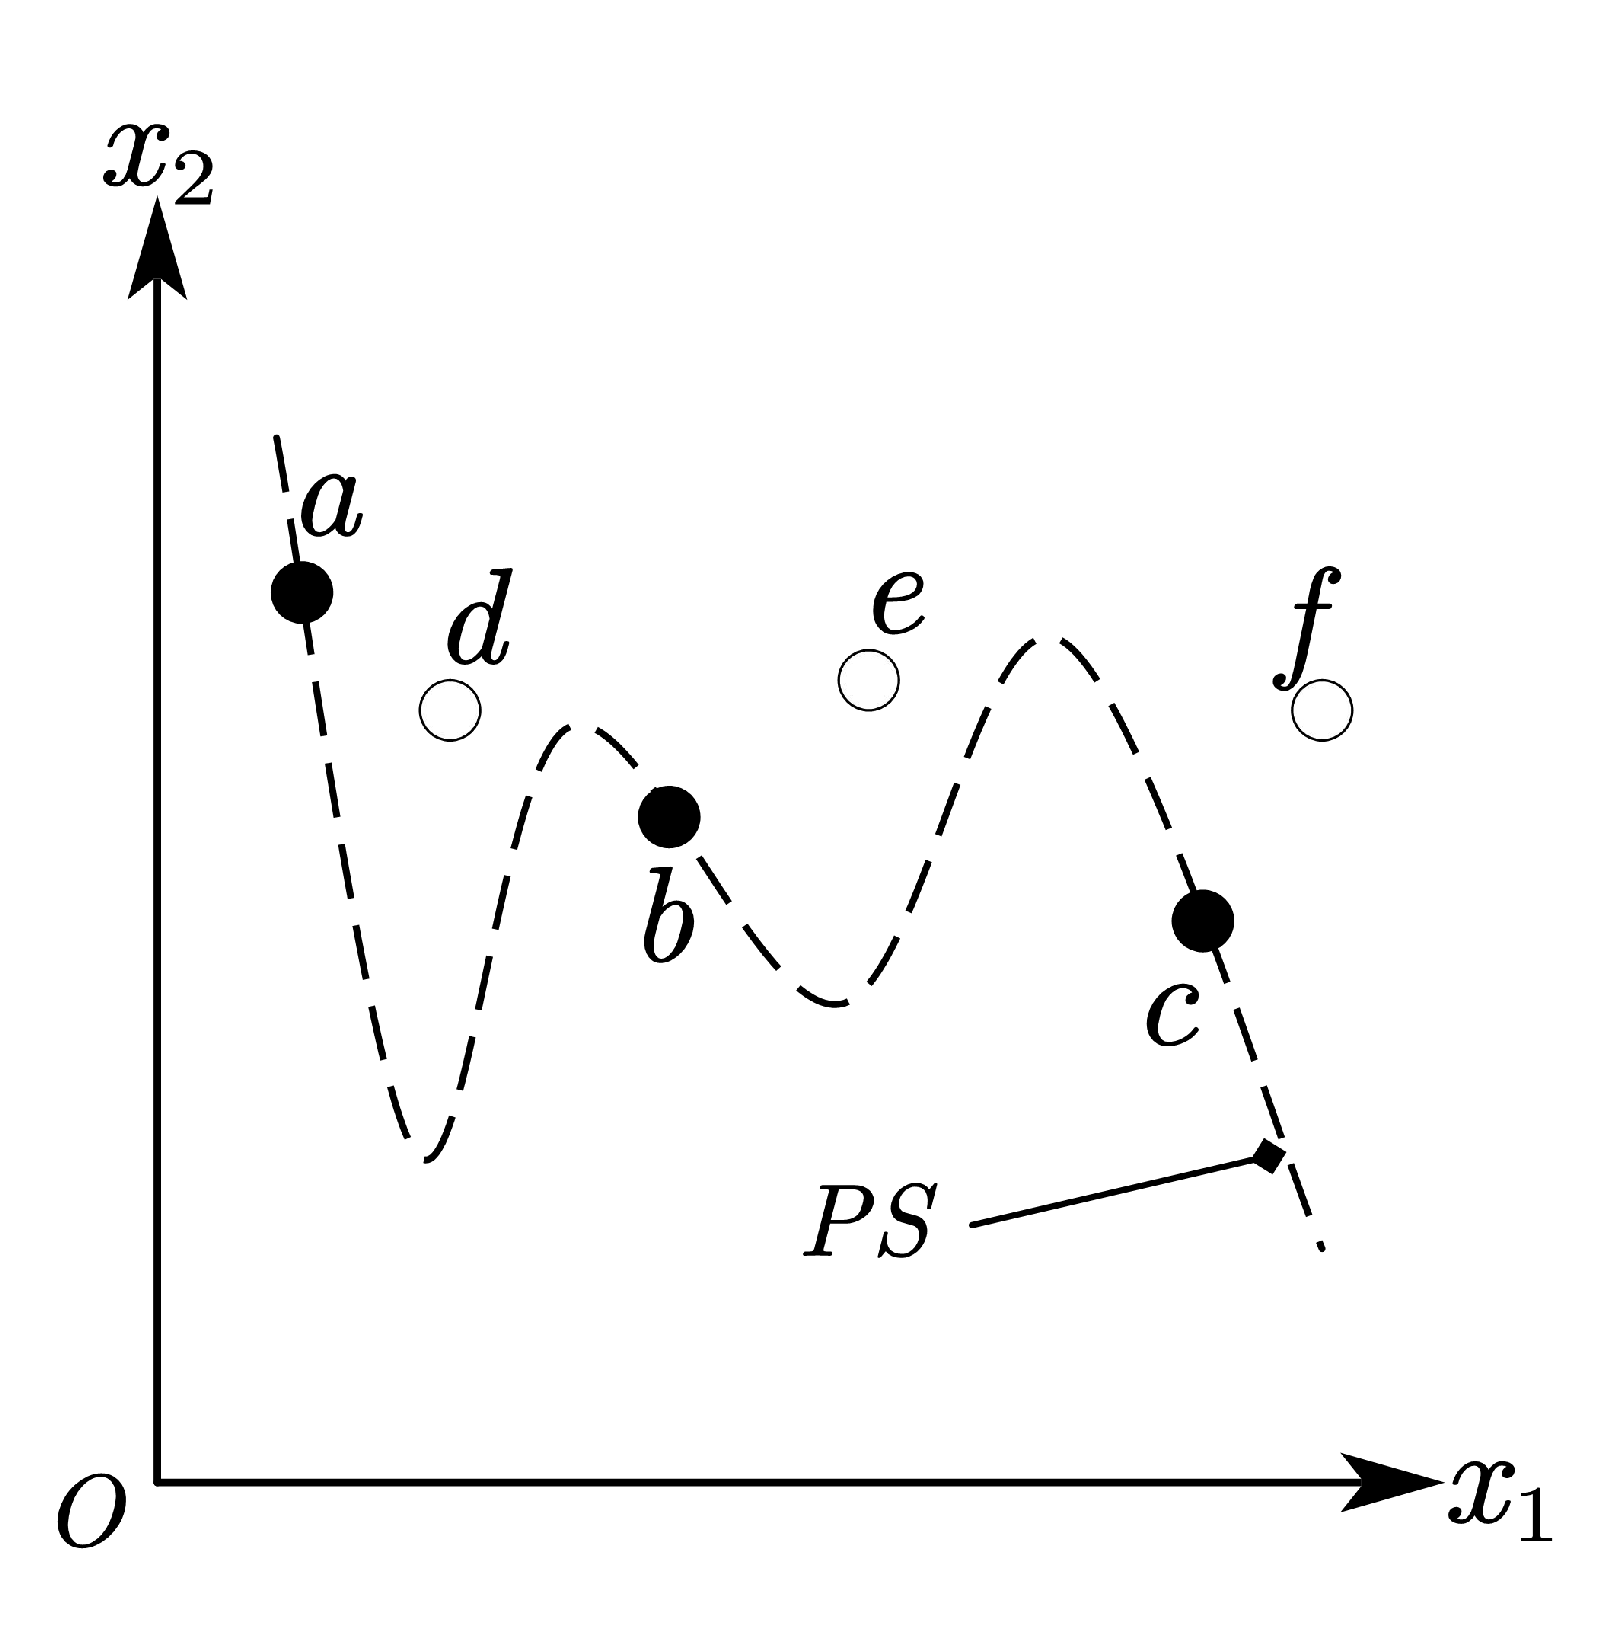
\includegraphics[width=.4\linewidth]{决策空间.pdf}}
    \subfloat[目标空间\label{subfig:目标空间}]{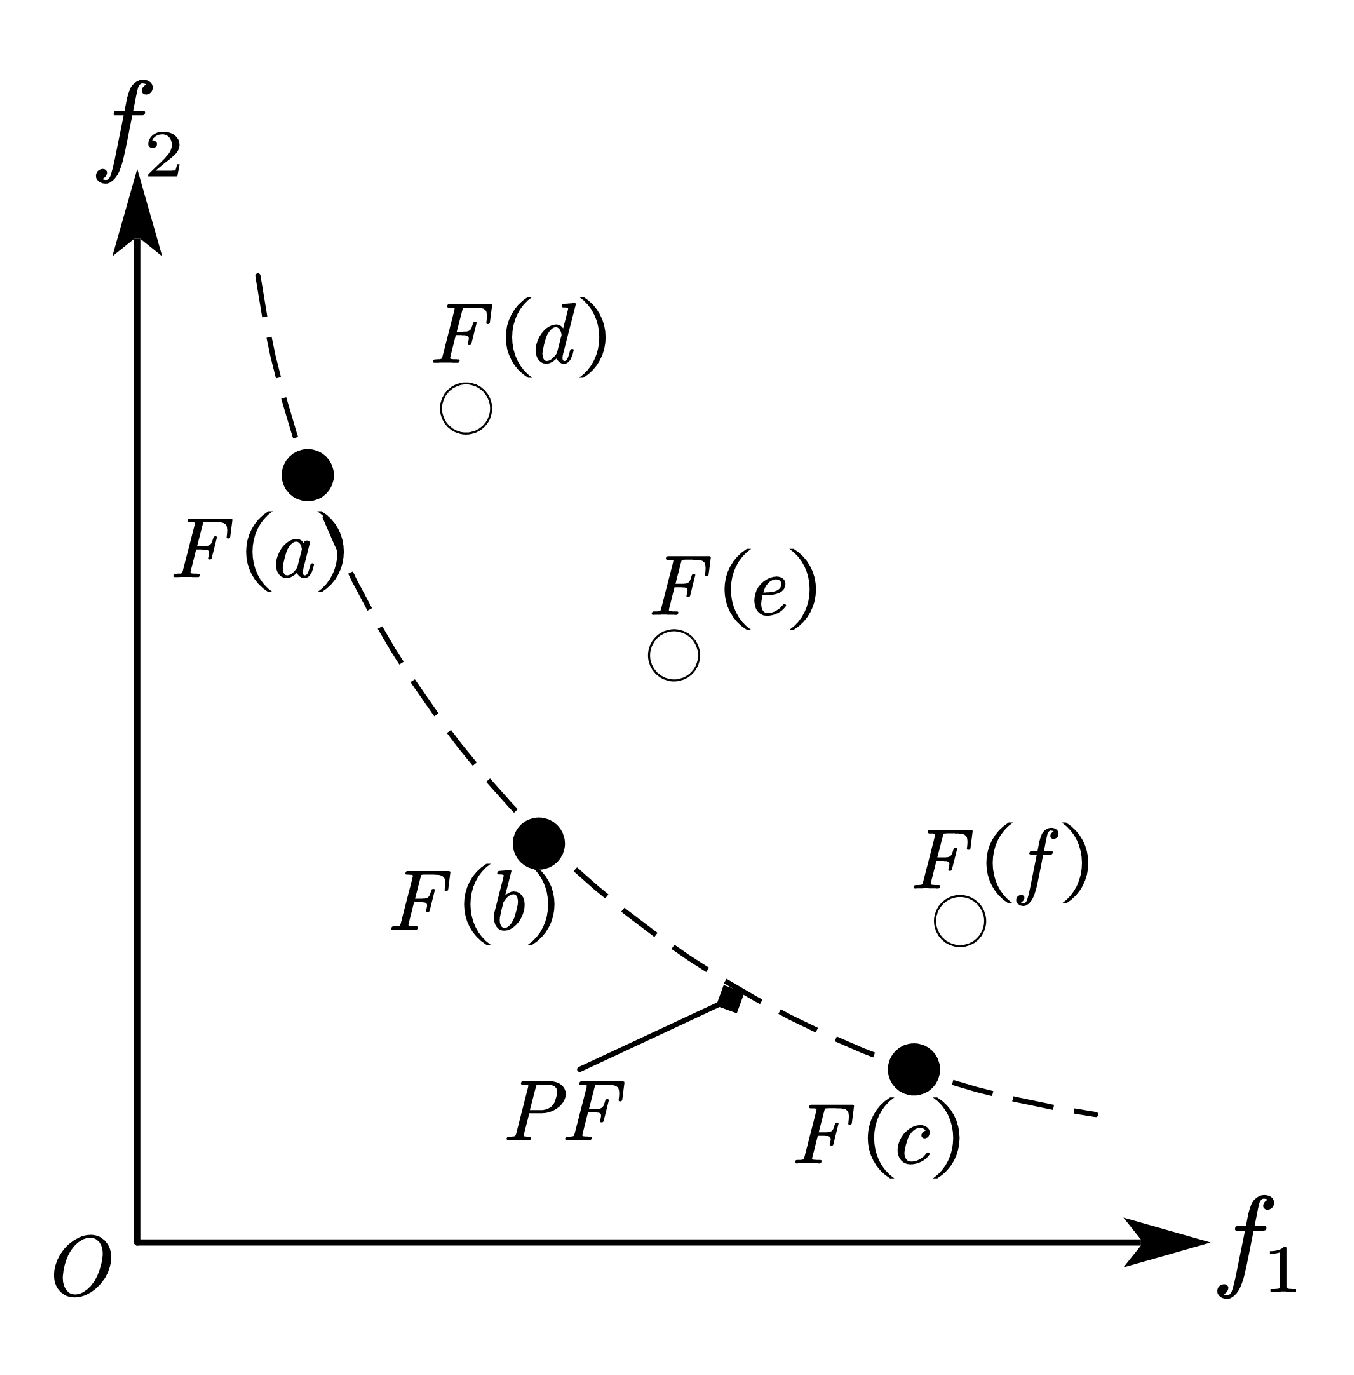
\includegraphics[width=.4\linewidth]{目标空间.pdf}}
    \caption{MOP中相关概念示意图}
    \label{fig:MOP中相关概念示意图}
\end{figure}
\par
设计多目标优化算法时,在目标空间中,还有两个比较重要的概念:理想点(Ideal Point)和边界点(Nadir Point),他们限定了PF的空间范围。
\par
\begin{definition}[理想点(Ideal Point)]
    \label{def:理想点}
    目标空间中,所有可行解$\mathbf{x} \in \Omega$在各个目标上的最小值构成的向量称为理想点(理想目标向量),记作$\mathbf{z}^* = \{ z_1^*, \cdots, z_m^* \}^T$,即
    \begin{align}
        \label{eq:理想点}
        z_i^* = \min_{x \in \Omega} f_i(\mathbf{x}), \ i \in \{ 1, \cdots, m \}.
    \end{align}
\end{definition}
\par
\begin{definition}[边界点(Nadir Point)]
    \label{def:边界点}
    目标空间中,PS中所有可行解$\mathbf{x}$在各个目标上的最大值构成的向量称为边界点(边界目标向量),记作$\mathbf{z}^{nad} = \{ z_1^{nad}, \cdots, z_m^{nad} \}^T$,即
    \begin{align}
        \label{eq:边界点}
        z_i^{nad} = \max_{x \in PS} f_i(\mathbf{x}), \ i \in \{ 1, \cdots, m \}.
    \end{align}
\end{definition}
\par
\begin{figure}[htb]
    \subfloat[2目标MOP\label{subfig:极值点-2D}]{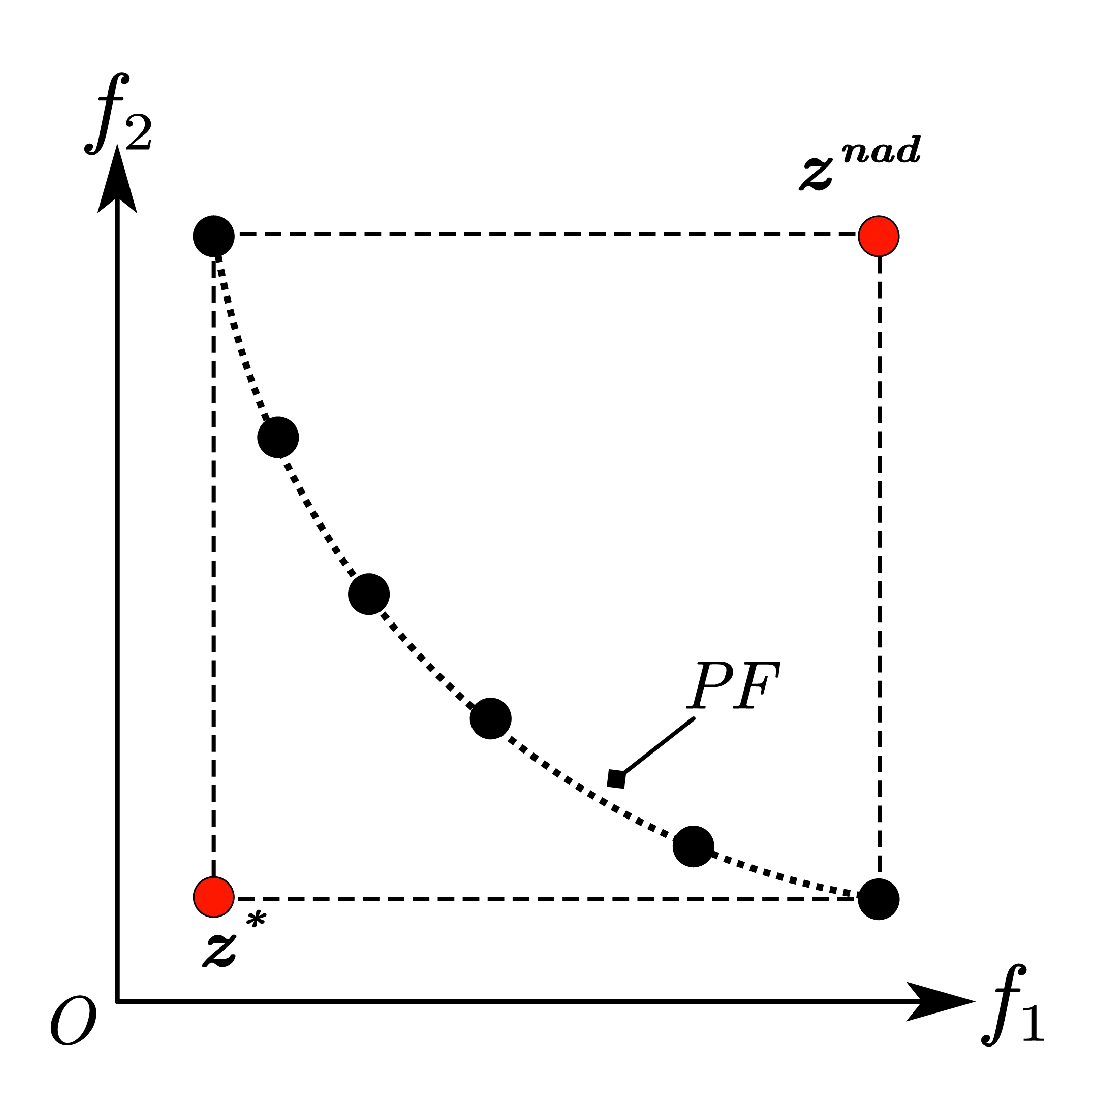
\includegraphics[width=.4\linewidth]{极值点-2D.pdf}}
    \subfloat[3目标MOP\label{subfig:极值点-3D}]{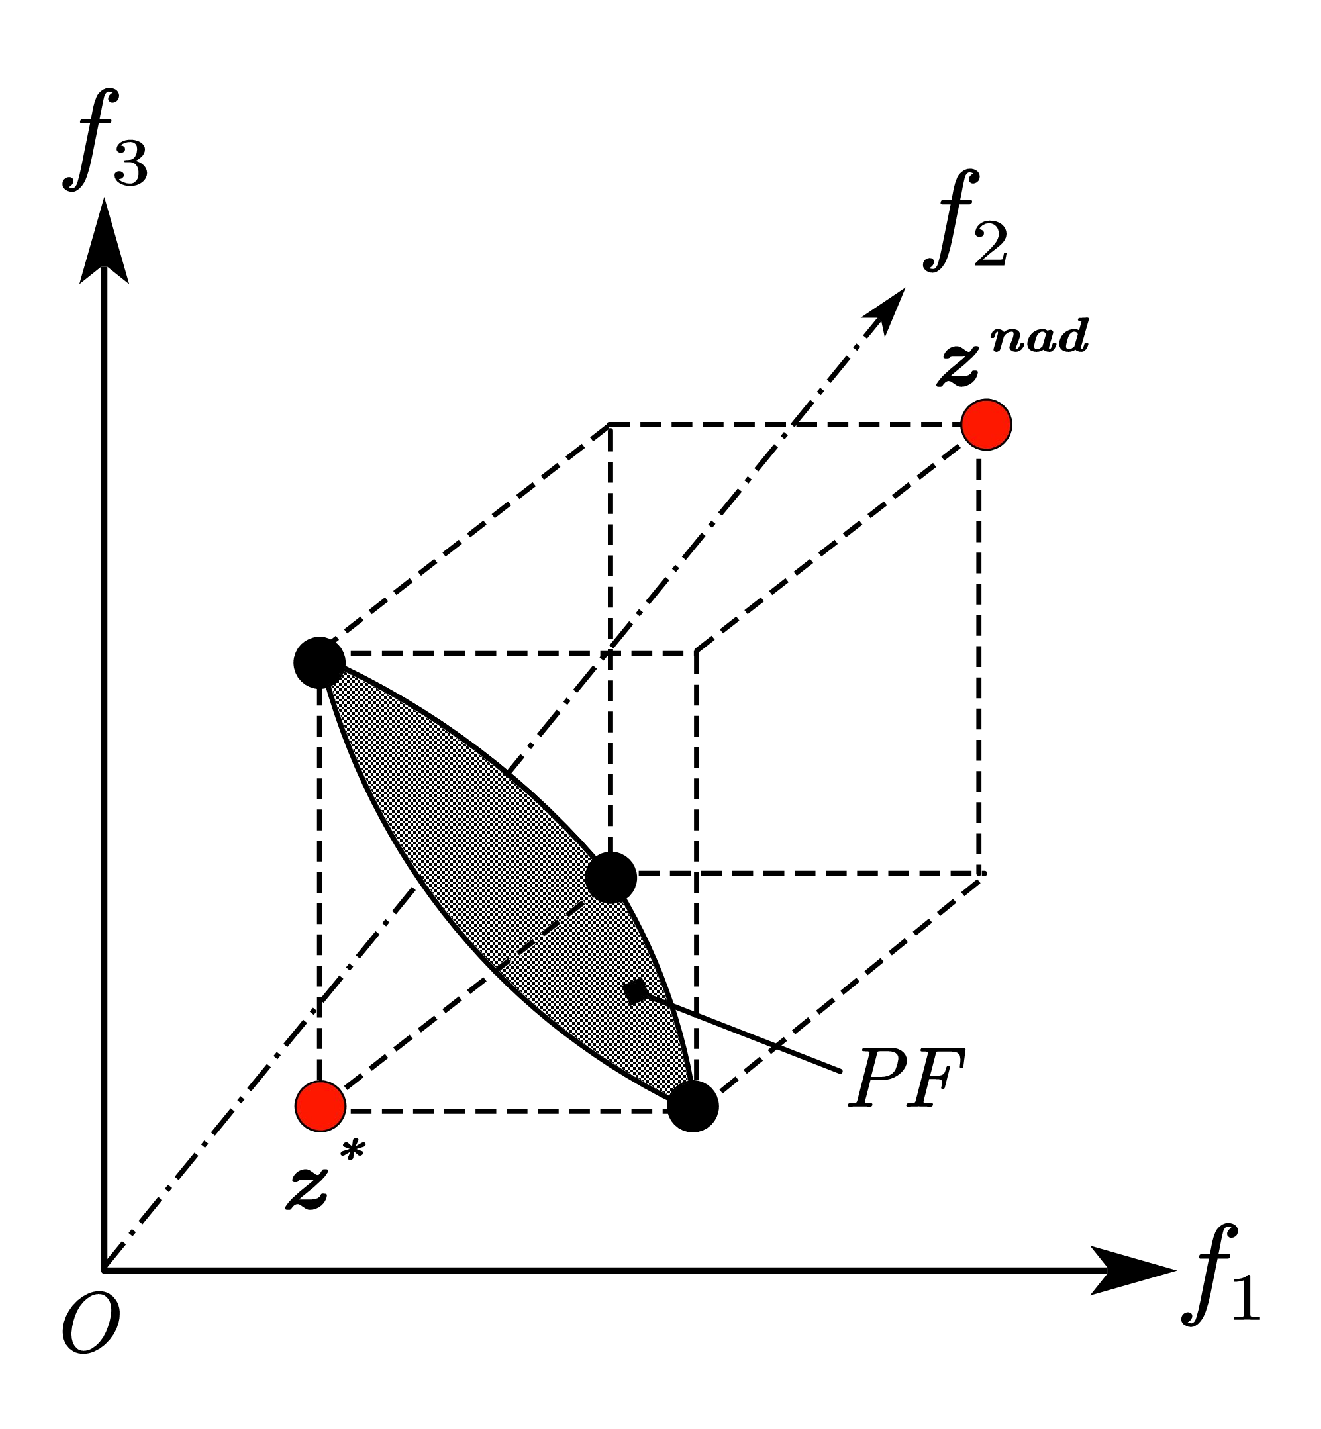
\includegraphics[width=.4\linewidth]{极值点-3D.pdf}}
    \caption{理想点和边界点示意图}
    \label{fig:理想点和边界点示意图}
\end{figure}
\par
如\autoref{fig:理想点和边界点示意图}~中所示,\autoref{subfig:极值点-2D}~和\autoref{subfig:极值点-3D}~分别为两目标和三目标MOP理想点和边界点示意图。由图可以看出,理想点和边界点限定了PF所在区域,分别确定其上下界。

\section{多目标组合优化算法}
\label{sec:背景介绍:多目标组合优化算法}
在大多数MOP中,都需要同时考虑多个互相冲突的目标,通常这些目标难以同时都达到最好的效果,其中一个目标的性能的提升往往会导致问题中的另外一个或多个目标的性能降低。这就需要在优化各个目标时进行权衡,这也致使算法最终求得的解不是惟一的,而是一组互不支配的解(非支配解集)。而这也是进化算法适合求解MOP的原因之一,进化算法正是一种基于群体(多个解)的迭代算法。对于进化算法而言,群体之间的信息遗传(共享)能够促进群体间个体的多元性,并且能够保证群体中的一些优秀信息能被下一代群体继承,进而使得整个群体进化(优化)。由此,本论文基础算法是基于进化算法的,并且,在本节中,首先介绍多目标进化算法的基本框架,然后会对一些多目标组合优化相关的优化技术进行详细介绍。

\subsection{进化算法}
\label{subsec:背景介绍:多目标组合优化算法:进化算法}
进化算法(EA)是一种无需太多问题的先验假设,使用种群循环迭代的方式来有效解决大规模问题的随机全局搜索算法。EA的主要指导思想是基于达尔文的进化论,通过适者生存、优胜劣汰的遗传机制来使得种群在表现出基因多样性的同时相互竞争,从而使得种群进化。EA正是通过模拟自然界物种的行为,在解空间随机的搜索可行解,产生后代种群的同时对种群进行适者生存、优胜劣汰的遗传操作,将高质量的可行解保留,低劣的解淘汰,从而保证算法是往最优解的方向逼近直至收敛。由于EA本身的高适应性和高扩展性的优点,EA可以与现有的启发式算法相组合,被广泛应用于求解各种优化问题。
\par
为了模拟自然界的物种进化,MOEA之中引入了个体、种群、适应度、遗传操作、选择策略等概念:
\begin{itemize}
    \item \textbf{个体:}在实际问题抽象成解空间后,将解编码成能表示其信息的向量(符号串),这个向量(符号串)就是个体。
    \item \textbf{种群:}个体的集合,进化的对象。
    \item \textbf{适应度:}度量个体对于环境的适应程度(个体的质量)。个体的适应度越高,说明该个体的生存能力越强。
    \item \textbf{遗传操作:}一般包括复制(Reproduction)、交叉(Crossover)和变异(Mutation)三种基本形式,是EA的核心部分。在算法中,通过设置三种算子起作用的概率,从而来控制整个群体的进化方向。
    \item \textbf{选择策略:}是从父代中挑选出子代种群的策略,常用的有非支配排序(Non-dominated Sort,NDSort)\cite{srinivas1994muiltiobjective,jensen2003reducing,tang2008fast,mcclymont2012deductive,zhang2014efficient}、拥挤距离(Crowding Distance)\cite{kundu2011multi}、精英保留等策略\cite{deb2002fast}或者混合策略。
\end{itemize}
\par
随着问题的不同,上述MOEA中的部件也会有所不同,我们通常需要根据具体的问题,设计出适用于对应问题的算子。其算法框架如下:
\begin{algorithm}
    \setstretch{1.5}
    \caption{多目标进化算法框架}
    \label{alg:多目标进化算法框架}
    \BlankLine
    \KwIn{ \\
        \hspace{1em} $\mathbf{MOP}$:多目标优化问题 \\
        \hspace{1em} $\mathbf{params}$:种群参数 \\
        \hspace{1em} $\mathbf{stop}$:终止条件
    }
    \KwOut{$\mathcal{PS}$}
    $\mathcal{P} \xleftarrow[]{\text{初始化}} \mathbf{MOP},\mathbf{params}$ \;
    \While{not $\mathbf{stop}$}{
        $\mathcal{P}^{'} \xleftarrow[]{\text{遗传操作}} \mathcal{P} $ \;
        $\mathcal{P}_{new} \leftarrow \mathcal{P} \bigcup \mathcal{P}^{'} $\;
        $fitness \xleftarrow[]{\text{适应度评价}} \mathcal{P}_{new} $ \;
        $\mathcal{P} \xleftarrow[fitness]{\text{选择策略}} \mathcal{P}_{new} $ \;
    }
    $\mathcal{PS} \xleftarrow[]{NDSort} \mathcal{P} $ \;
    \textbf{return } $\mathcal{PS}$ \;
\end{algorithm}
\par
\begin{figure}[htb]
    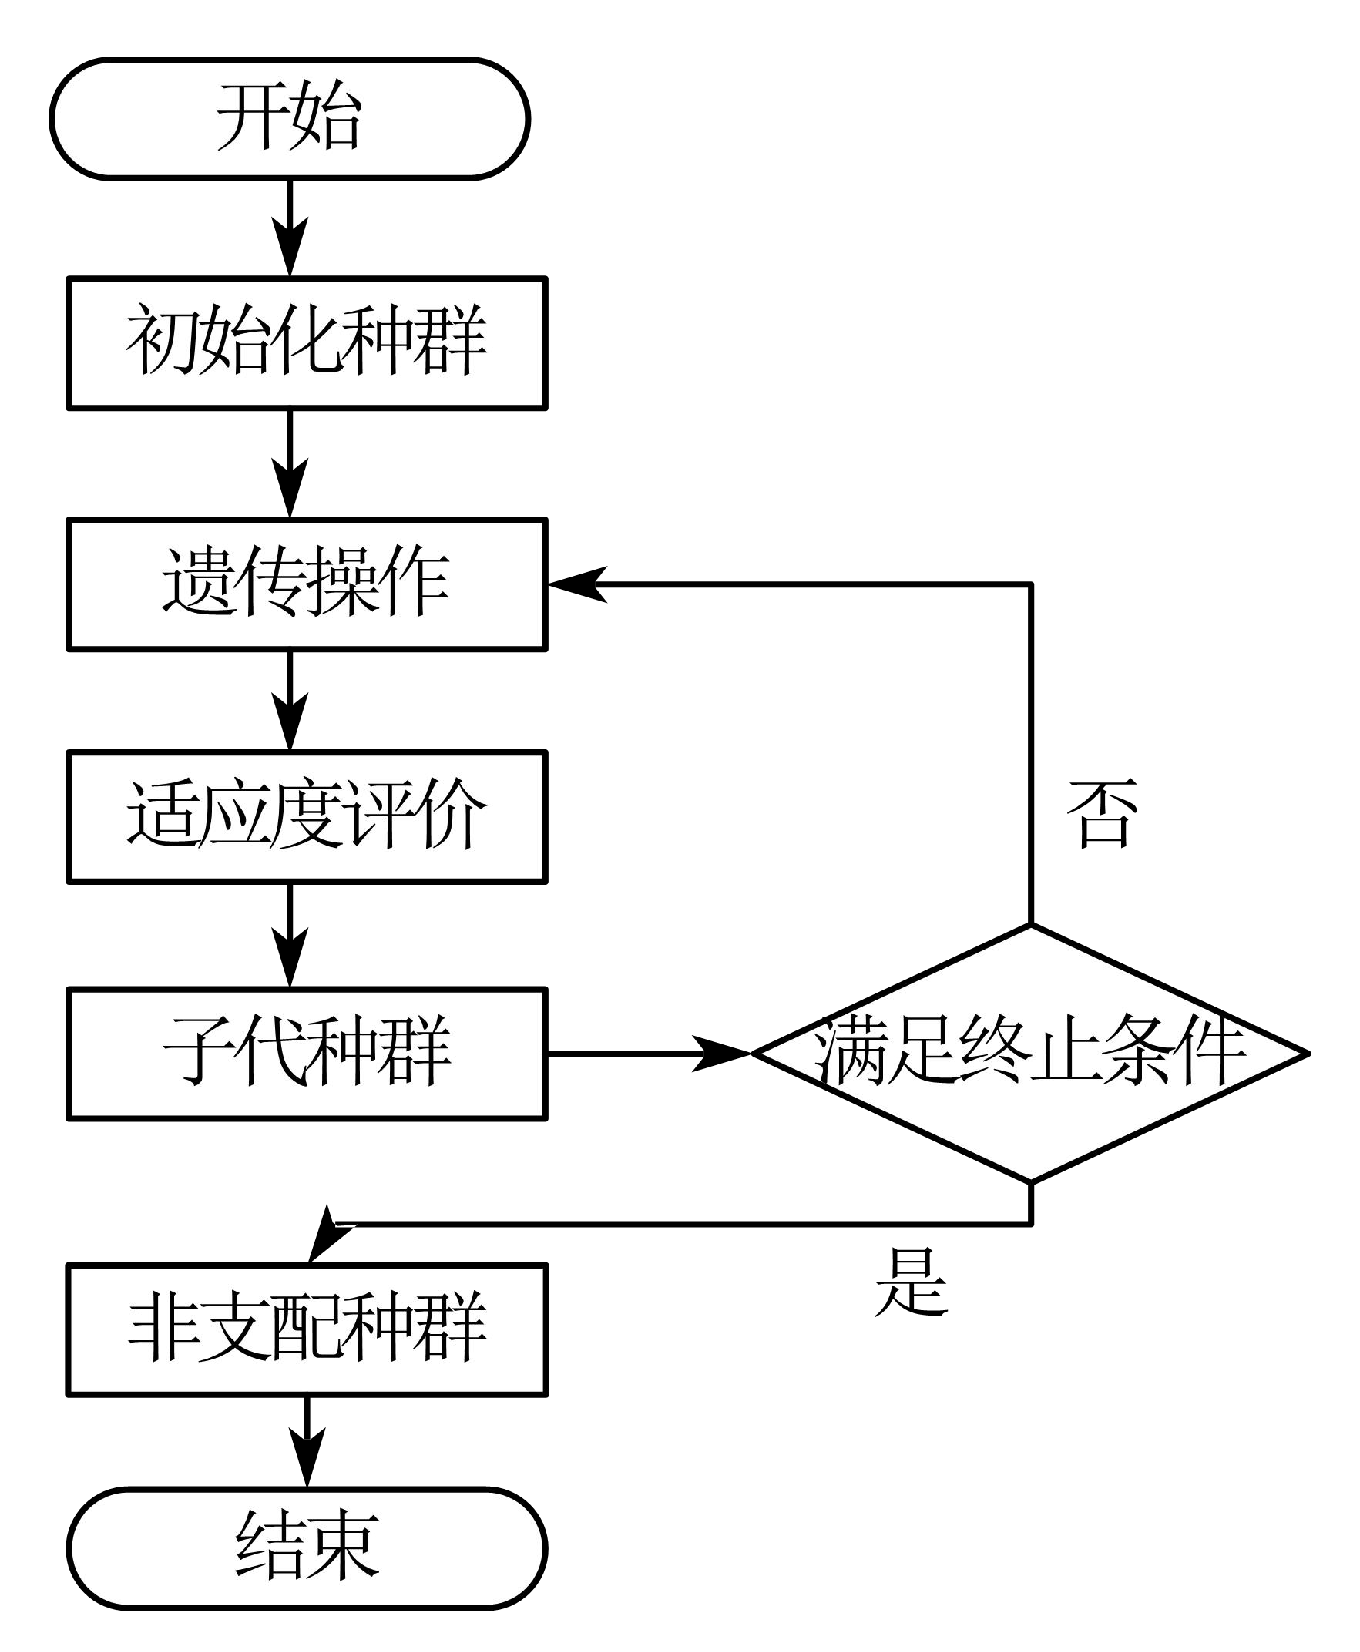
\includegraphics[width=.5\linewidth]{多目标进化算法流程.pdf}
    \caption{多目标进化算法流程图}
    \label{fig:多目标进化算法流程图}
\end{figure}
\par
算法\ref{alg:多目标进化算法框架}~是多目标进化算法的基本框架,与\autoref{fig:多目标进化算法流程图}~展示的多目标进化算法流程图相对应。在算法中,首先随机初始化一个种群$\mathcal{P}$,$\mathcal{P}$中的个体即为问题的初始解,个体是根据MOP而设计的向量或符号串,种群规模根据$\mathbf{params}$而设置。接下来就是迭代过程,模拟的是种群的进化。然后对种群$\mathcal{P}$进行遗传操作(对于不同的问题,遗传操作也不尽相同。组合优化通常采用局部搜索的方式产生新的个体,局部搜索算子也需要单独设计)产生新的种群$\mathcal{P}^{'}$,接着将父代种群和新产生的种群混合,获取它们所有个体的评价值,然后根据评价值和选择策略选出子代种群(选择策略通常采用的是精英选择策略,是算法中至关重要的一步,它需要确保种群能够向着好的方向进化,即向PF逼近,同时还需要兼顾多样性和收敛性这两个关键指标)。最后在末代的时候,采用非支配排序的方式,从种群$\mathcal{P}$中选出非支配种群$\mathcal{PS}$。
\par
由算法\ref{alg:多目标进化算法框架}~和\autoref{fig:多目标进化算法流程图}~展示的多目标进化算法的工作流程,可以清晰的知道,如何产生和挑选子代种群是我们需要关注的对象。但是,没有在算法\ref{alg:多目标进化算法框架}~和\autoref{fig:多目标进化算法流程图}~中体现的细节,也是我们研究的重点。比如:
\begin{itemize}
    \item 设计容易表达问题的个体
    \item 算法终止的条件
    \item 局部搜索算法(产生新个体的方法,设计问题的邻域结构)
\end{itemize}

\subsection{基于分解的多目标进化算法}
\label{subsec:背景介绍:多目标组合优化算法:基于分解的多目标进化算法}
1985年,Fourman和Schaffer等人在解决多目标优化问题时提出多目标进化算法\cite{fourman1985compaction,schaffer1985multiple},经由多年的研究发展,已经衍生出各种各样的多目标进化算法,按照不同的策略大致可以归纳为三类算法框架:基于支配的(Domination-based)、基于分解的(Decomposition-based)和基于指标的(Indicator-based)多目标进化算法。尽管基于支配的和基于指标的多目标进化算法框架仍然被广泛的使用,但是由于各自算法机制的原因,导致他们在很多方面有着的局限性。基于支配的多目标进化算法框架的缺陷在于它不适用于超多目标(优化目标数$m > 3$)的优化问题,在超多目标优化问题的解集中,几乎所有的解之间都是非支配的,这使得非支配排序算法几乎失效,导致算法中的选择策略不能为种群进化提供有效的指导,最终导致算法不能向PF逼近,不能起到优化的作用\cite{ishibuchi2008behavior,giagkiozis2015methods}。同样,基于指标的多目标进化算法框架的其中一个局限性是,它依赖于指标的计算,然而大多数指标的计算复杂度会随着问题目标的数量呈指数级增长,这导致算法难以在有效时间内使用,如基于超体积指标的多目标进化算法,其计算复杂度随目标数呈指数上升,即使目前有很多能够降低复杂度的近似方法,也不能满足多目标优化问题的效率需求。
\par
近年来,在对多目标进化算法的研究中,基于分解的多目标进化算法越来越受到研究者们的关注,其核心思想是通过分解的方式,将一个多目标优化问题分解为一组单目标的子问题,然后使用优化算法对这些单目标子问题同时进行优化,最后将这些单目标子问题的解组合成一个多目标优化问题的解集。在早期,分解的思想就在解决多目标优化问题的几个启发式算法中得到了一定程度上的应用\cite{ishibuchi1998multi,jin2001adapting,jaszkiewicz2002performance,paquete2003two,hughes2003multiple}。2007年,Zhang等人结合分解的思想,系统的提出了基于分解的多目标进化算法(MOEA/D)\cite{zhang2007moea},成为了最热门的基于分解的多目标进化算法之一。近来更是涌现出各种基于MOEA/D的算法框架,被用来解决各种各样的多目标优化问题\cite{ke2013moea,ke2014hybridization}。
\par
在MOEA/D中,它把一个多目标优化问题根据一组权重向量分解成多个单目标子问题,然后根据各个子问题之间的联系形成邻居关系,然后利用邻居子问题之间的信息对所有子问题进行优化。对于一个具有$m$个目标的MOP,我们将其分解成$k$个子问题,首先需要定义$k$个均匀的权重向量,其中一个权重向量$\boldsymbol{\lambda}$为:
\begin{align}
    \label{eq:权重向量}
    \boldsymbol{\lambda} = (\lambda_1, \cdots. \lambda_m)^T, \quad \forall \lambda_i \geq 0 , \quad \sum_{i=1}^m \lambda_i = 1. 
\end{align}
然后,针对不同类型的问题,我们可以是使用不同的分解方法,下面将介绍三种常用的分解方法(聚合函数):
\par
\begin{enumerate}
    \item \textbf{加权和法(Weight Sum,WS):}WS是一种常用的线性多目标优化问题的聚合方法\cite{hillermeier2001nonlinear},它的目标函数聚合形式为可定义为:
    \begin{align}
        \label{eq:WS}
        minimize \quad & g^{ws}(\mathbf{x} \ | \ \boldsymbol{\lambda}) = \sum_{i=1}^m \lambda_i f_i(\mathbf{x}), \\
        subject \ \ to \quad & \mathbf{x} \in \Omega. \notag
    \end{align}
    其中$\mathbf{x}$是决策向量,$\boldsymbol{\lambda}$为权重向量。
    \begin{figure}[htb]
        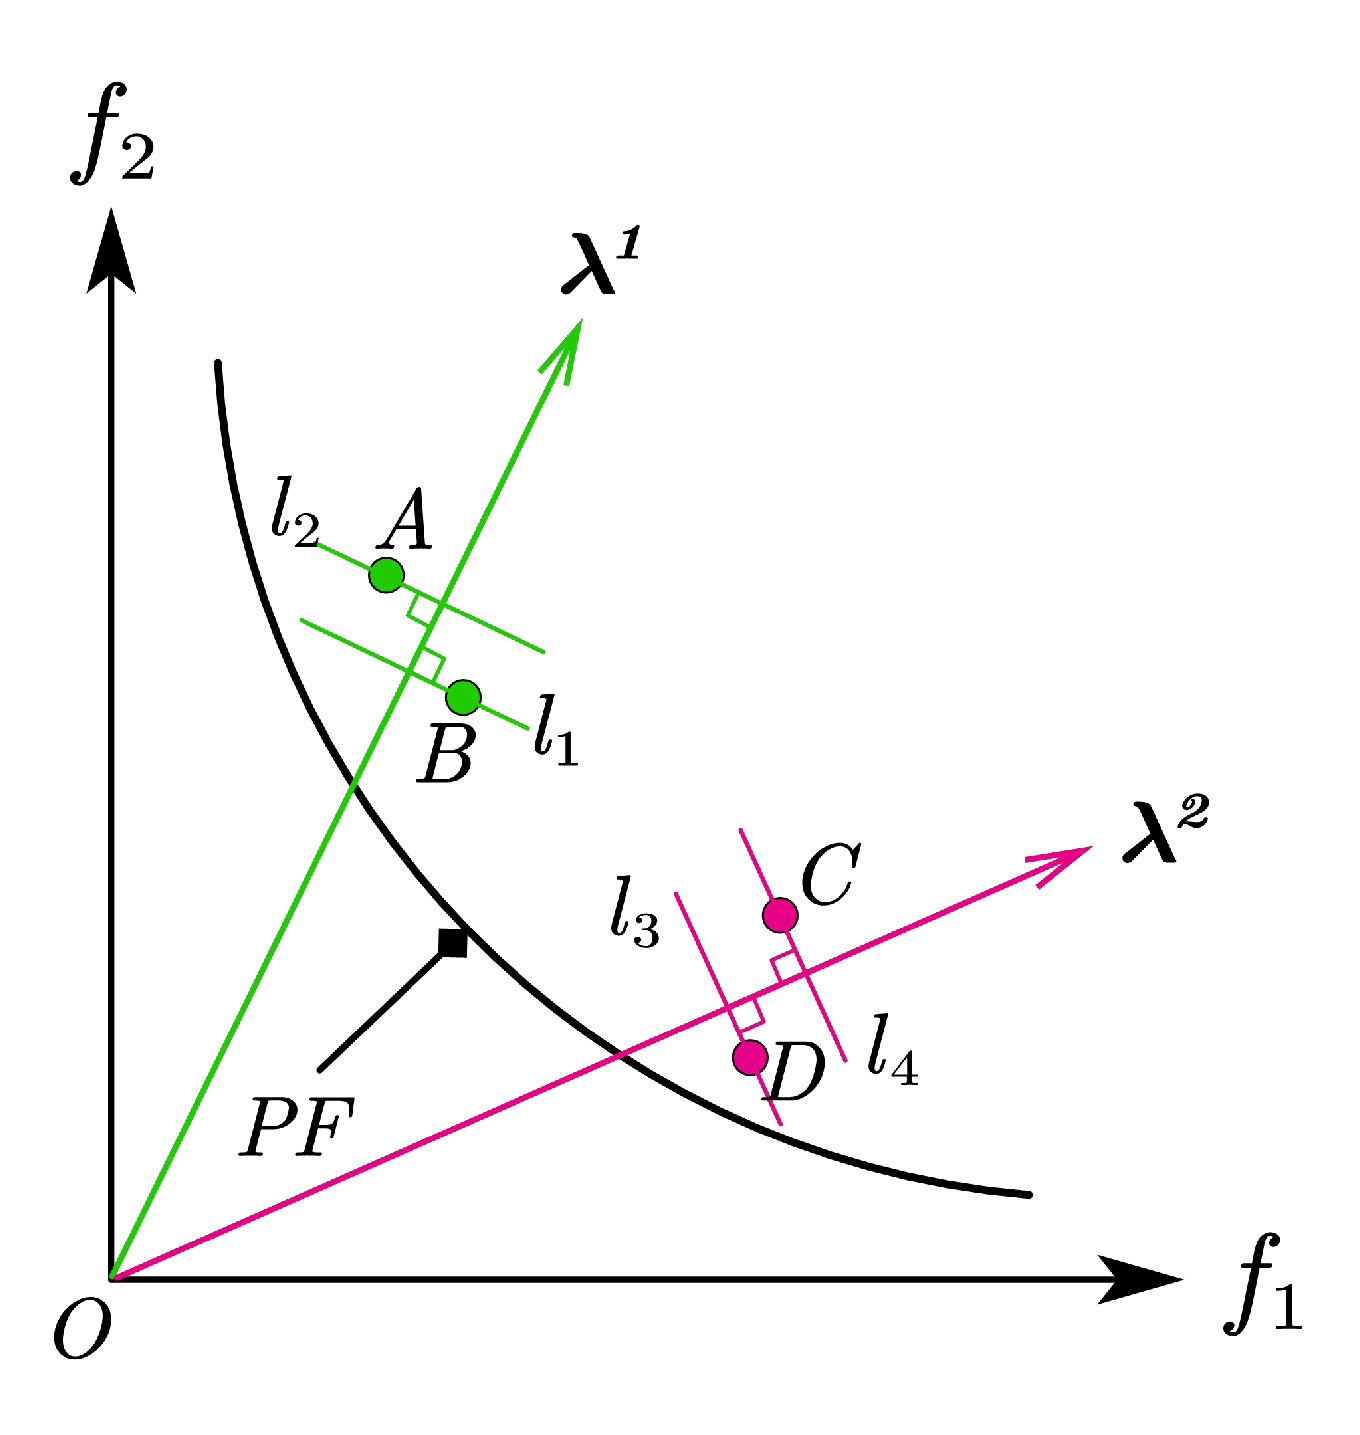
\includegraphics[width=.45\linewidth]{WS等高线.pdf}
        \caption[加权和法(WS)等高线示意图]{加权和法(WS)等高线示意图 \\ $\boldsymbol{\lambda^1}$和$\boldsymbol{\lambda^2}$分别为两个子问题的权重向量,$l_1, l_2, l_3, l_4$分别为对应子问题的等高线}
        \label{fig:WS等高线示意图}
    \end{figure}
    \par
    \autoref{fig:WS等高线示意图}~展示的是一个二目标优化问题使用加权和法的等高线示意图。容易看出,加权和法的等高线是一簇与权重向量$\boldsymbol{\lambda}$垂直的平行直线。个体在权重向量上的投影长度即为该个体在所属$\boldsymbol{\lambda}$上的子问题的聚合值。在\autoref{fig:WS等高线示意图}~中,个体A和B是互不支配的,但是,在$\boldsymbol{\lambda^1}$所属子问题上用加权和法后,个体B要优于个体A,因为个体B在$\boldsymbol{\lambda^1}$上的投影长度要比个体A短。同理,个体D优于个体C。
    \item \textbf{切比雪夫法(Tchebycheff,TCH):}TCH是一种非线性多目标聚合方法\cite{jaszkiewicz2002performance},它的目标函数聚合形式可定义为:
    \begin{align}
        \label{eq:TCH}
        minimize \quad & g^{tch}(\mathbf{x} \ | \ \boldsymbol{\lambda},\mathbf{z}^*) = \max_{1 \leq i \leq m} \lambda_i | f_i(\mathbf{x}) - z^*_i |, \\
        subject \ \ to \quad & \mathbf{x} \in \Omega. \notag
    \end{align}
    其中$\mathbf{x}$是决策向量,$\boldsymbol{\lambda}$为权重向量,$\mathbf{z}^*$为理想点(\autoref{def:理想点})。
    \par
    \begin{figure}[htb]
        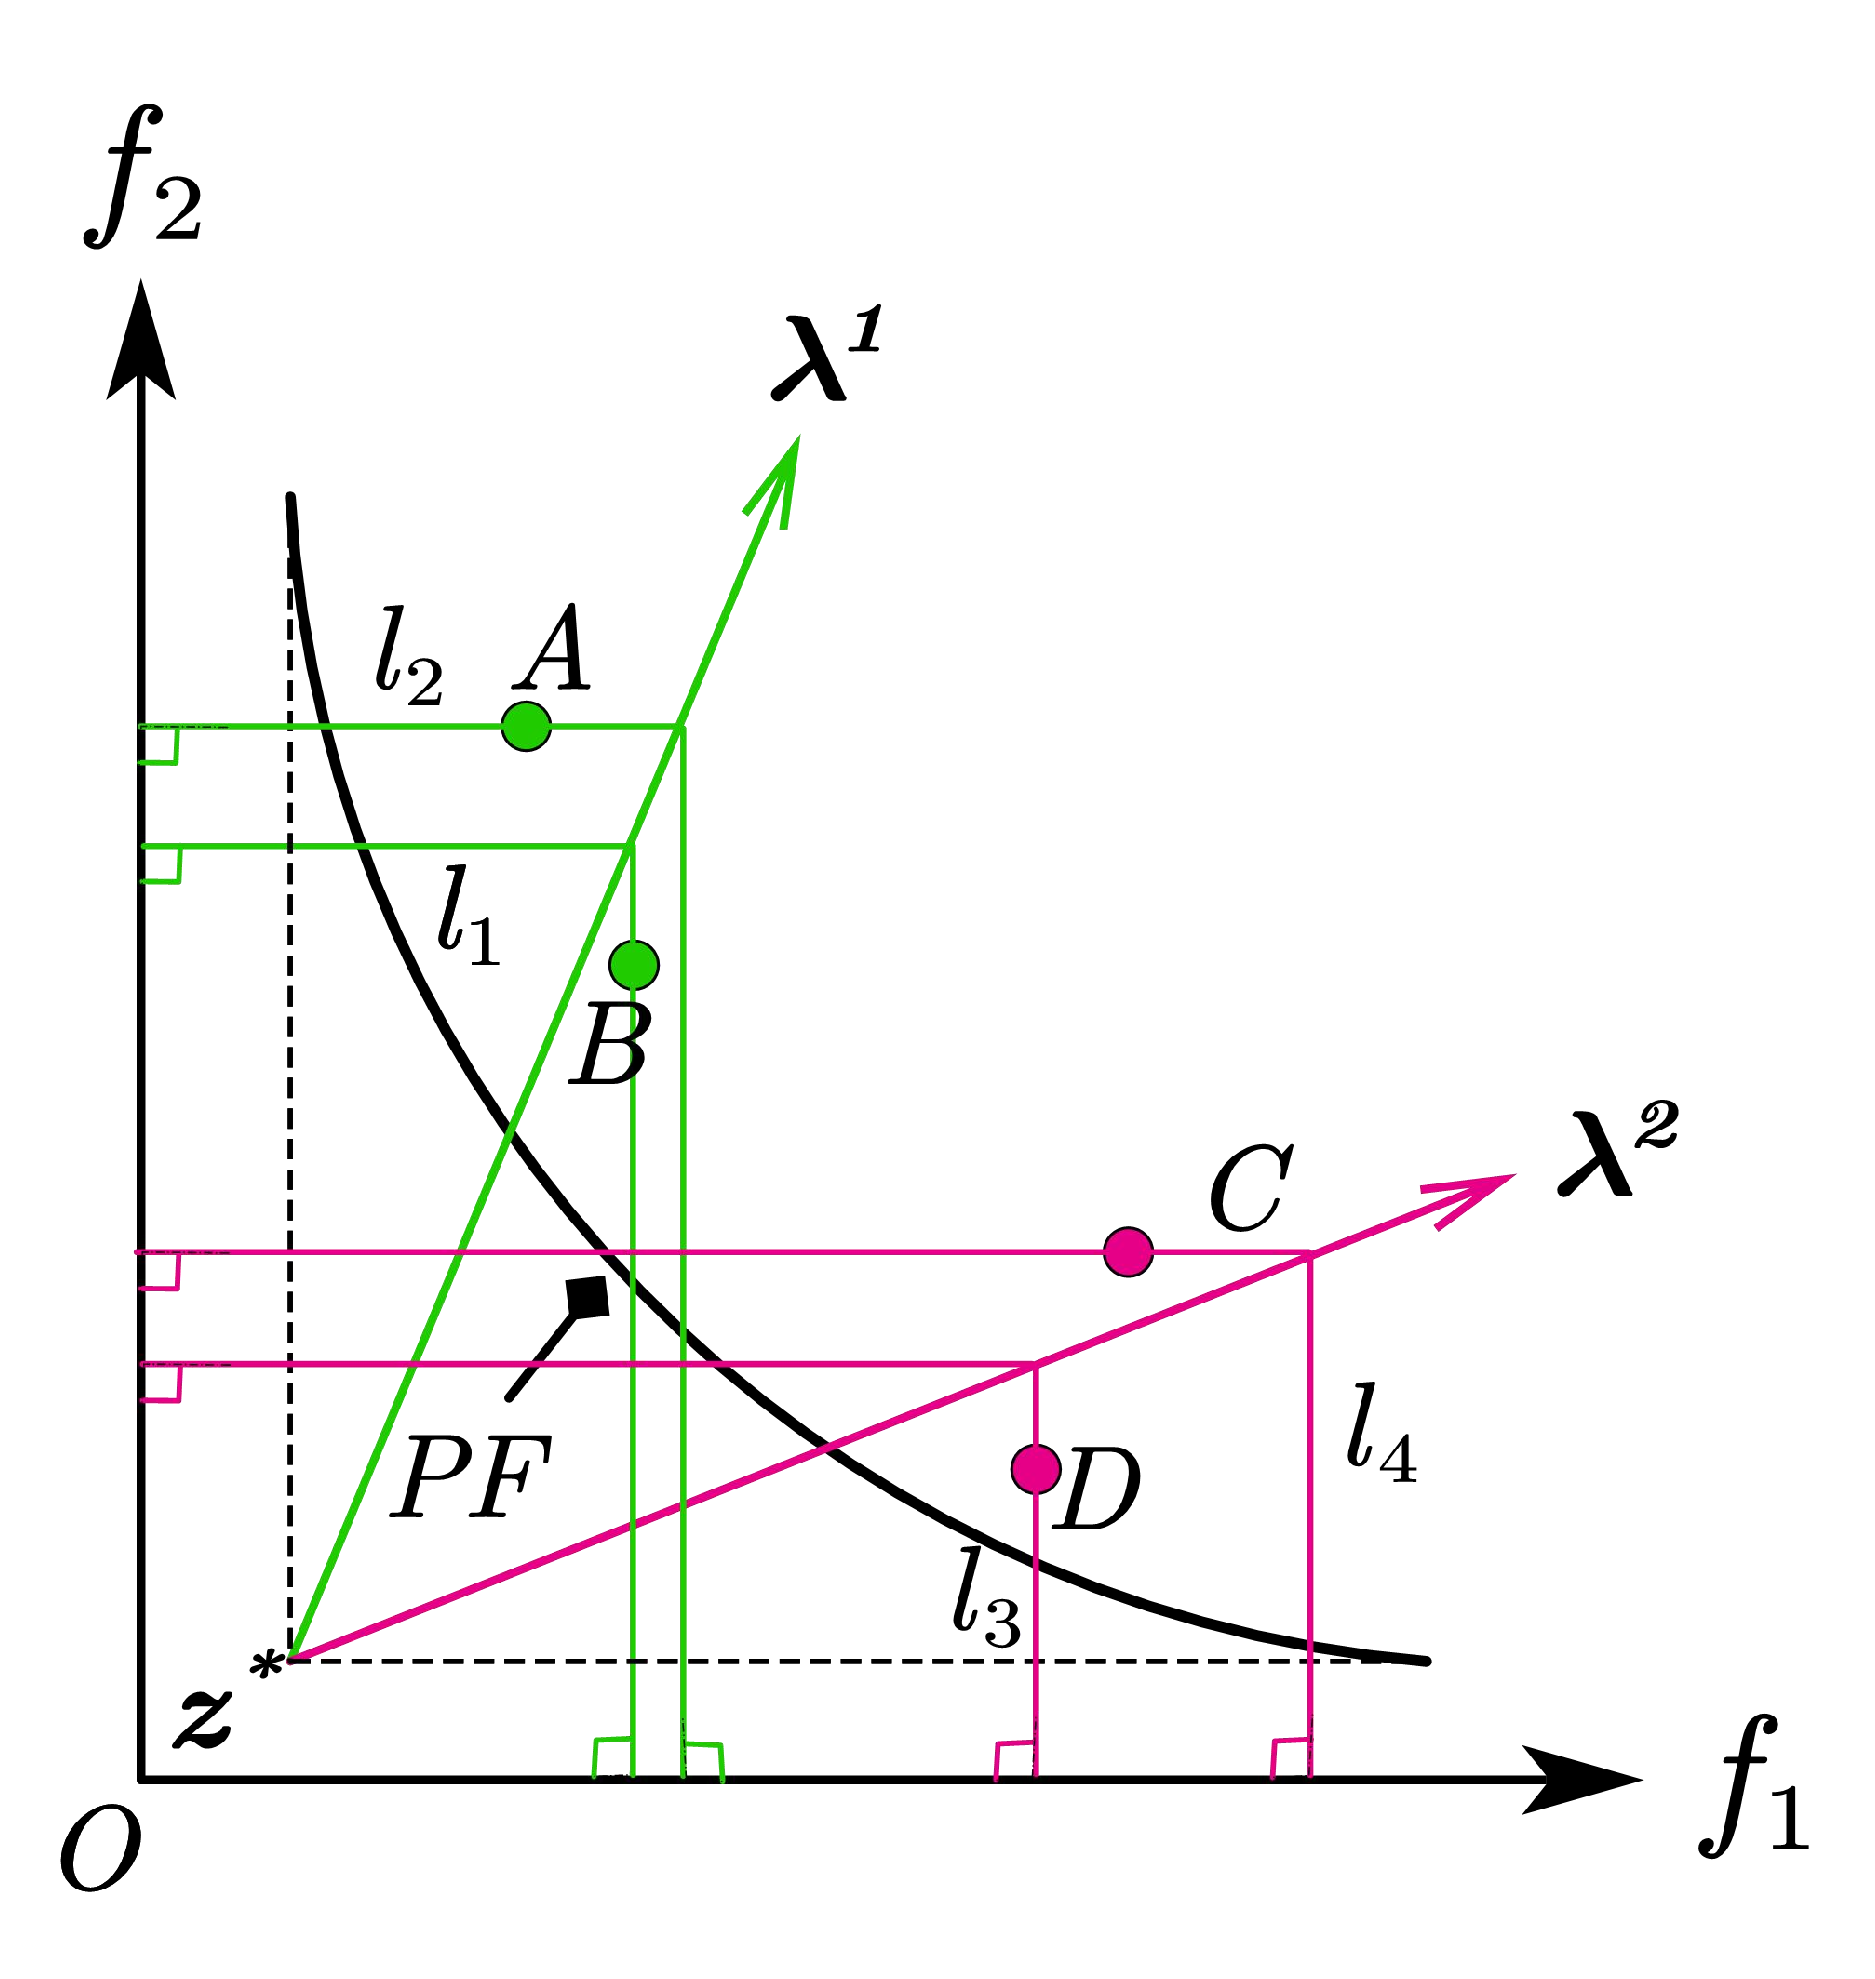
\includegraphics[width=.45\linewidth]{TCH等高线.pdf}
        \caption[切比雪夫法(TCH)等高线示意图]{切比雪夫法(TCH)等高线示意图 \\ $\boldsymbol{\lambda^1}$和$\boldsymbol{\lambda^2}$分别为两个子问题的权重向量,$l_1, l_2, l_3, l_4$分别为对应子问题的等高线}
        \label{fig:TCH等高线示意图}
    \end{figure}
    \par
    \autoref{fig:TCH等高线示意图}~展示的是一个二目标优化问题使用切比雪夫法的等高线示意图。从\autoref{fig:TCH等高线示意图}~中可以看出,对于$\boldsymbol{\lambda^1}$所属子问题,个体B优于个体A,因为个体B的切比雪夫聚合值要优于个体A。同理,个体D优于个体C。从图中还可以分析出,在连续PF时,用TCH分解方法得到的子问题的最优解是权重向量与PF面的交点。在非连续PF时,由于权重向量可能和PF面没有交点,所属不同权重向量的子问题可能具有相同的最优解。相比于加权和法,TCH分解方法的等高线沿着权重向量呈直角锯齿形,因此,用TCH方法得到的子问题具有更小的收敛区域(搜索空间),这在处理高维问题时,TCH分解方法能够很好的限制收敛区域,因此能够很好的保证种群的收敛性。
    \item \textbf{基于惩罚的边界交叉法(Penalty-based Boundary Intersection,PBI):}PBI是由Zhang等人于2007年提出的一种分解方法\cite{zhang2007moea},它的目标函数聚合形式为:
    \begin{align}
        \label{eq:PBI}
        minimize \quad & g^{pbi}(\mathbf{x} \ | \ \boldsymbol{\lambda},\mathbf{z}^*) = d_1 + \theta d_2, \\
        & d_1 = \frac{\| (\mathbf{z}^* - F(\mathbf{x}))^T \boldsymbol{\lambda} \Vert }{ \|  \boldsymbol{\lambda} \Vert }, \notag\\
        & d_2 = \| F(\mathbf{x}) - (\mathbf{z}^* - d_1 \boldsymbol{\lambda}) \Vert, \notag \\
        subject \ \ to \quad & \mathbf{x} \in \Omega. \notag
    \end{align}
    其中$\mathbf{x}$是决策向量,$\boldsymbol{\lambda}$为权重向量,$\mathbf{z}^*$为理想点(\autoref{def:理想点}),$d_1$表示目标向量$F(\mathbf{x})$到权重向量$\boldsymbol{\lambda}$的投影长度,$d_2$表示目标向量$F(\mathbf{x})$到权重向量$\boldsymbol{\lambda}$的垂直距离,$\theta$为惩罚因子,用于调节$d_1$和$d_2$之间的平衡,控制种群的分布性和收敛性。
    \par
    \begin{figure}[htb]
        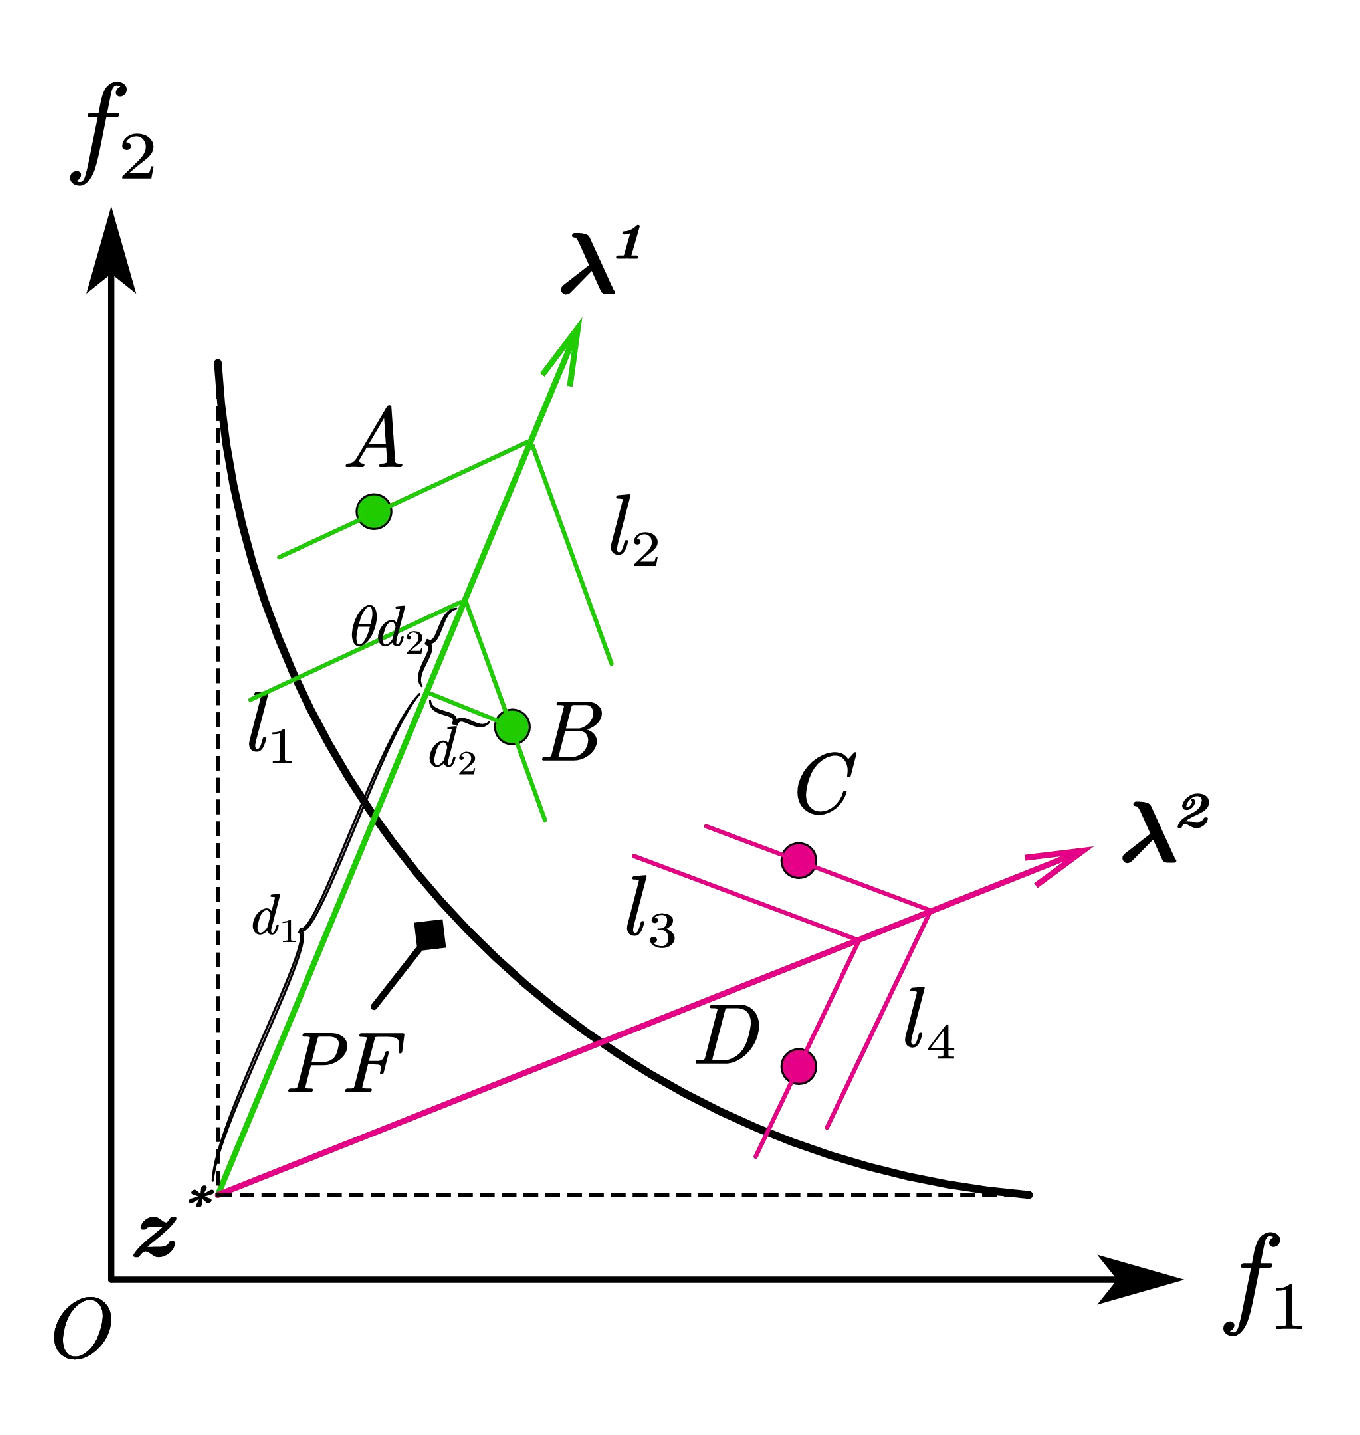
\includegraphics[width=.45\linewidth]{PBI等高线.pdf}
        \caption[基于惩罚的边界交叉法(PBI)等高线示意图]{基于惩罚的边界交叉法(PBI)等高线示意图 \\ $\boldsymbol{\lambda^1}$和$\boldsymbol{\lambda^2}$分别为两个子问题的权重向量,$l_1, l_2, l_3, l_4$分别为对应子问题的等高线}
        \label{fig:PBI等高线示意图}
    \end{figure}
    \par
    \autoref{fig:PBI等高线示意图}~展示的是一个二目标优化问题使用基于惩罚的边界交叉法的等高线示意图。在图中,$d_1$是个体B到权重向量$\boldsymbol{\lambda^1}$的投影长度,$d_2$是个体B到权重向量$\boldsymbol{\lambda^1}$的垂直距离,$d_1+\theta d_2$即为PBI聚合值。显然,对于$\boldsymbol{\lambda^1}$所属子问题,个体B的PBI聚合值要优于个体A,即个体B优于个体A。同理,个体D优于个体C。通过\autoref{eq:PBI}~和\autoref{fig:PBI等高线示意图}~可以知道,PBI能够通过调节$\theta$参数来控制$d_1$和$d_2$之间的平衡,从而控制种群的分布性和收敛性。由于能够控制分布性和收敛性之间的平衡这一特点,PBI分解方法在处理高维目标(超多目标)问题时具有很大的优势。但是,参数$\theta$的设置也影响着算法的性能表现,这同时也成为PBI分解方法的缺点之一。
\end{enumerate}
\par
MOEA/D算法的核心思想是将MOP分解成一系列单目标子问题或者多个多目标子问题,然后利用这些子问题的邻域相似度,通过协作的方式来同时优化所有子问题,从而向PF逼近。通常子问题有权重向量通过聚合函数确定,这些子问题之间的邻域关系是通过各个子问题的权重向量之间的相似度(欧式距离)来度量的。与其他的多目标进化算法不同的是,MOEA/D算法注重从当前子问题的邻域子问题中选择父个体,通过遗传算子(交叉、变异算子)来生成新个体,并且按照一定的策略来更新邻域中的种群。因此,一个优秀的基于邻域的优化策略能够确保MOEA/D算法的搜索效率。在算法的迭代进化过程中,一旦搜索到针对某个子问题的高质量解,这个解的优质信息就会迅速的被邻域内的其他个体继承,从而加快整个种群进化(收敛)的速度。下面是MOEA/D算法的一个基本框架流程:
\begin{algorithm}[ht]
    \caption{MOEA/D算法框架}
    \label{alg:MOEA/D算法框架}
    \BlankLine
    \KwIn{ \\
        \hspace{1em} $\mathbf{MOP}$:多目标优化问题 \\
        \hspace{1em} $\mathbf{N}$:子问题个数 \\
        \hspace{1em} $\mathbf{T}$:邻域大小 \\
        \hspace{1em} $\boldsymbol{\lambda}$:一组均匀分布的权重向量 $\{ \boldsymbol{\lambda^1}, \cdots, \boldsymbol{\lambda^N} \}$\\
        \hspace{1em} $\mathbf{stop}$:终止条件
    }
    \KwOut{$\mathcal{EP}$:外部集(精英种群)}
    $\mathcal{SP} = \{ SP_1, \cdots, SP_N \} \xleftarrow[\mathbf{N}]{\boldsymbol{\lambda}} \mathbf{MOP}$ \;
    $\mathbf{B}(i) = \{ i_1, \cdots, i_T \}, i \in \{ 1, \cdots, N \}$,其中$\{ \boldsymbol{\lambda}^{i_1}, \cdots, \boldsymbol{\lambda}^{i_T} \}$是最接近$\boldsymbol{\lambda}^i$的$\mathbf{T}$个权重向量 \;
    $\mathcal{P} \xleftarrow[]{\mathbf{N}} $随机生成大小为$\mathbf{N}$的初始种群 \;
    $\mathbf{z}^* \leftarrow $通过\autoref{eq:理想点}更新理想点 \;
    \While{not $\mathbf{stop}$}{
        \For{$i = \{1, \cdots, \mathbf{N}\} $}{
            $\mathbf{x}^{'} \xleftarrow[]{\text{遗传算子}}$ 由$SP_i$的邻居$\mathbf{B}(i)$确定$\mathcal{P}$中的两个个体 \;
            $\mathbf{z}^* \leftarrow$ 用$F(\mathbf{x}^{'})$更新理想点 \;
            通过聚合函数(式\ref{eq:WS},\ref{eq:TCH},\ref{eq:PBI}),用$\mathbf{x}^{'}$更新$SP_i$的邻居解 \;
            $\mathcal{EP} \leftarrow$ 用$F(\mathbf{x}^{'})$更新外部集 \;
        }
    }
    \textbf{return } $\mathcal{EP}$ \;
\end{algorithm}
\par
算法\ref{alg:MOEA/D算法框架}~可以分为三个阶段:初始化、遗传生成和更新阶段。在初始化阶段,首先将MOP通过权重向量分解成$\mathbf{N}$个子问题$\mathcal{SP} = \{ SP_1, \cdots, SP_N \}$,并且初始化每个子问题的邻居,然后随机生成初始种群$\mathcal{P}$,并得到理想点$\mathbf{z}^*$。在遗传生成阶段主要是从邻居中选出父代个体,然后通过遗传操作来生成子代个体$\mathbf{x}^{'}$。最后的更新阶段就是用生成的子代个体$\mathbf{x}^{'}$来更新邻居解、理想点和外部集。应该注意的是,算法中邻域的大小和替换个体的次数会对种群的分布性和收敛性产生影响。并且在更新阶段,外部集$\mathcal{EP}$中保存着所有被搜索到的非支配解,为了节省资源,可以用一些已有的密度估计方法来控制外部集$\mathcal{EP}$的大小。

\section{局部搜索}
\label{sec:背景介绍:局部搜索}
搜索算法是有目的的穷举一个问题解空间中部分或者所有的可能情况,直到搜索到问题的解的一种方法,实际上是根据初始条件和扩展规则构造一颗解答树并寻找符合目标状态节点的过程。从宏观上看,所有的搜索算法都可以划分为两个部分:控制结构(扩展点的方式)和生成系统(扩展节点),而大多数的算法优化和改进都主要是通过修改控制结构来完成的。
\par
在全局搜索(Global Search,GS)中,需要将所有搜索到的路径都记录下来,直到搜索到最优解(满意解),其中,到达目标状态的搜索路径就是问题的解。但是,在大多数问题中,绝大多数的的搜索路径与最终目标状态并不是紧密相关的。因此,没有必要将所有搜索到的路径都记录下来,只需要关键路径即可,这样能够节省大量的空间和时间。与GS记录所有搜索路径相对,只维护当前目标状态和记录部分关键搜索路径的搜索算法就是局部搜索算法(Local Search,LS)。当问题的状态空间(决策空间)很大时,全局搜索算法就不适用了,其找到最优解所需的时间和空间都将成指数形式的增长,因此,设计效率高的局部搜索算法也是我们研究的重点。并且,本文主要的研究载体是多目标组合优化问题,这类问题的决策空间是离散的,并且十分巨大,导致往常用的遗传算子(交叉、变异等)生成新个体的效率低下。因此,应对这类问题,局部搜索算子就成了算法中必不可缺的一部分。

\subsection{基本概念}
\label{subsec:背景介绍:局部搜索:基本概念}
对于一个组合优化问题,局部搜索算法就是在该问题的候选解空间(邻域结构)上进行搜索,其搜索过程是从选择初始的候选解开始,然后在当前候选解的邻域结构中进行搜索,如此迭代直到找到一个满意的解或者搜索到了局部搜索算法的终止条件。在搜索过程中,每次对候选解是否被选择的决策仅基于有限的局部信息,并且算法中的决策和最开始的初始化可以是随机的。因此,基于以上局部搜索算法过程,可以给定以下定义\cite{blum2003metaheuristics}:
\begin{definition}
    \label{def:CO}
    给定一个最小化CO问题$P = (\mathcal{S}, f)$,变量$\mathbf{x}=\{ x_1, \cdots, x_n \} \in \mathcal{X}$,$\mathcal{X}$是离散有限(可数无限)变量集,其决策域为$\mathcal{D} = \{ D_1, \cdots, D_n \}$,约束域为$\mathcal{C}$,则有
    \begin{align}
        \label{eq:CO}
        minimize \quad & f: D_1 \times \cdots \times D_n \rightarrow \mathbb{R}^+, \\
        s.t. \quad & \mathcal{C}. \notag
    \end{align}
    则所有可能的可行解可表示为:
    \begin{align}
        \label{eq:可行解}
       \mathcal{S} = & \{ s = \{ (x_1, v_1), \cdots, (x_n, v_n) \} \}, \\
        s.t. \quad & v_i \in D_i, \ x_i \in \mathbf{x} \in \mathcal{X}, \ s \xrightarrow[]{s.t.} \mathcal{C}. \notag
        % & x_i \in \mathbf{x} \in \mathcal{X}, \notag \\
        % & s \xrightarrow[]{s.t.} \mathcal{C}. \notag
    \end{align}
    其中,$\mathcal{S}$被称为搜索(解)空间,因为集合中的每个元素都可以看作是一个候选解。要解决CO问题,需要在搜索空间$\mathcal{S}$中找到能够使得目标函数$f$值最小的解$s^* \in \mathcal{S}$,即$f(s^*) \leq f(s), \forall s \in \mathcal{S}$。$s^*$称为$(\mathcal{S}, f)$的全局最优解。
\end{definition}
\par
\begin{definition}
    \label{def:邻域动作和邻域}
    在局部搜索算法中,邻域动作是一个函数:
    \begin{align}
        \label{eq:邻域动作}
        \mathcal{N}:\mathcal{S} \rightarrow 2^{\mathcal{S}}.
    \end{align}
    对于解空间中任意一个解$\forall s \in \mathcal{S}$,有
    \begin{align}
        \label{eq:邻域}
        \mathcal{N}(s) \subseteq \mathcal{S}.
    \end{align}
    其中,$\mathcal{N}(s)$就是$s$的邻域。
\end{definition}
\par
\begin{definition}
    \label{def:局部最优解}
    对于一个邻域动作$\mathcal{N}:\mathcal{S} \rightarrow 2^{\mathcal{S}}$,在搜索空间$\mathcal{S}$中,有解$\hat{s}$,使得$\forall s \in \mathcal{N}(\hat{s}) : f(\hat{s}) \leq f(s)$,则称$\hat{s}$为局部最优解。如果$f(\hat{s}) < f(s), \forall s \in \mathcal{N}(\hat{s})$,则称$\hat{s}$为严格局部最优解。
\end{definition}
\par
\begin{algorithm}
    \caption{局部搜索算法框架}
    \label{alg:局部搜索算法框架}
    \BlankLine
    \KwIn{ \\
        \hspace{1em} $P = (\mathcal{S}, f)$ \\
        \hspace{1em} $\mathcal{N}:\mathcal{S} \rightarrow 2^{\mathcal{S}}$ \\
        \hspace{1em} $\mathcal{A}$:接受策略 \\
        \hspace{1em} $\mathbf{stop}$:终止条件
    }
    \KwOut{$s^*$}
    $s^* = (s \leftarrow \text{初始化})$ \;
    \While{not $\mathbf{stop}$}{
        \ForEach{$s^{'} \in \mathcal{N}(s)$}{
            $s^* \xleftarrow[]{s^{'} \prec s^*} s^{'}$ \;
            \If{$\mathcal{A}(s^{'}, s)$}{
                $s \leftarrow s^{'}$ \;
            }
        }
    }
    \textbf{return } $s^*$ \;
\end{algorithm}
\par
通过\autoref{def:CO}~,\autoref{def:邻域动作和邻域}~,\autoref{def:局部最优解}~和算法\ref{alg:局部搜索算法框架}~可以知道,通过邻域动作和邻域,可以产生对应解的邻居解集合,在迭代优化时,可以通过一定的策略来判断是否接受邻居解集合中的某个解,从而更新当前解。假设每次都接受比当前解更优的邻居解,那么当前解每次都能得到改进,这能够使得算法快速收敛到局部最优。

\subsection{邻域结构}
\label{subsec:背景介绍:局部搜索:邻域结构}
由章节\ref{subsec:背景介绍:局部搜索:基本概念}~可以知道邻域决定一个局部搜索算法的搜索效率和最终解的质量。邻域越小,搜索空间也会变得很小,局部搜索算法只需要搜索部分解空间就会很快收敛,这很大程度上节省了计算时间。但是,这并不能保证最终的局部最优解也足够的好,因为当邻域足够小时,解空间很大可能会不包含全局最优解或者优质的局部最优解,这使得算法不能搜索到优质的解。若邻域足够大,解空间包含了全局最优解或者优质局部最优解,但是算法需要花大量的计算量和时间去搜索到这个优质解。因此,综合以上原因,我们的目的是要根据具体的问题,找到一个邻域,使得这个邻域不仅足够的小,而且尽可能多的包含优质的局部最优解,我们称这样的邻域为邻域结构。
\par
一般地,邻域结构是建立在具体问题的基础之上的。并且,本文研究的主要内容也与邻域结构相关。因此,为保证一致性,在本文中,具体的问题和测试用例统一使用旅行商问题(Traveling Salesman Problem,TSP)和多目标旅行商问题(Multi-Objective Traveling Salesman Problem,MOTSP)(参考章节\ref{subsec:背景介绍:测试问题:MOTSP})。对于TSP问题,它的邻域是一个(全连接图)邻接矩阵,其中每个顶点的邻域是所有与该顶点相连的顶点。这个邻域中还包含了其他顶点的邻域,这些邻域中的顶点可以是与该顶点相邻的顶点,也可以是其他顶点的邻域。下面给出邻域结构的定义:
\begin{definition}[邻域结构(Neighborhood Structure,NS)]
    \label{def:邻域结构}
    邻居结构是每个顶点只与少数几个顶点相连(候选集(Candidate Set, CSet))的稀疏图,记作$\mathcal{N}$。
\end{definition}
% 分图
\begin{figure}[htb]
    \subfloat[全连接图$\mathcal{G}$ \label{subfig:全连接图}]{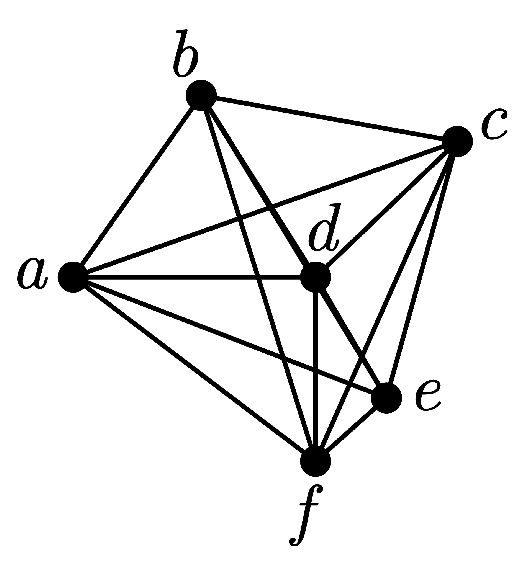
\includegraphics[width=.33\linewidth]{邻域结构-完全图.pdf}}
    \subfloat[邻居结构$\mathcal{N}_1$ \label{subfig:邻域结构1}]{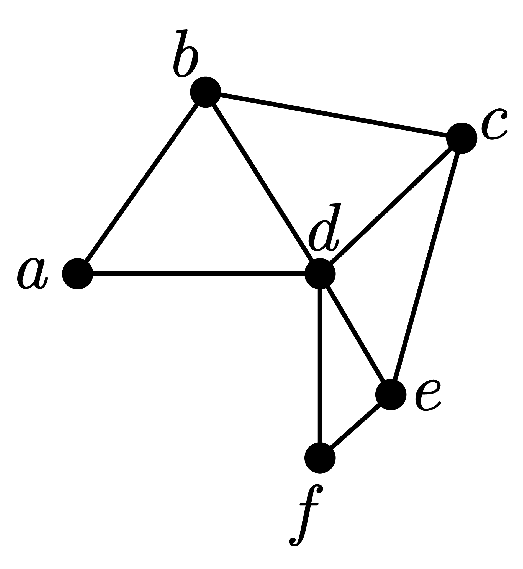
\includegraphics[width=.33\linewidth]{邻域结构-N1.pdf}}
    \subfloat[邻居结构$\mathcal{N}_2$ \label{subfig:邻域结构2}]{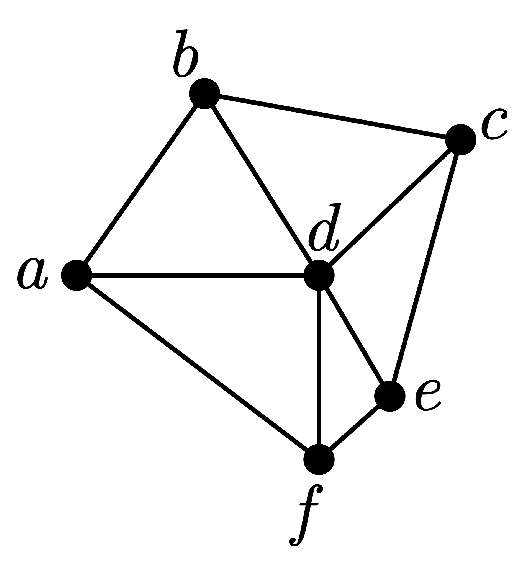
\includegraphics[width=.33\linewidth]{邻域结构-N2.pdf}}
    \caption[邻域结构示意图]{邻域结构示意图}
    \label{fig:邻域结构示意图}
\end{figure}
\begin{figure}[htb]
    \ContinuedFloat
    \subfloat[局部最优解$s^* \in \mathcal{N}_1 \in \mathcal{G}$ \label{subfig:邻域结构1-局部最优解}]{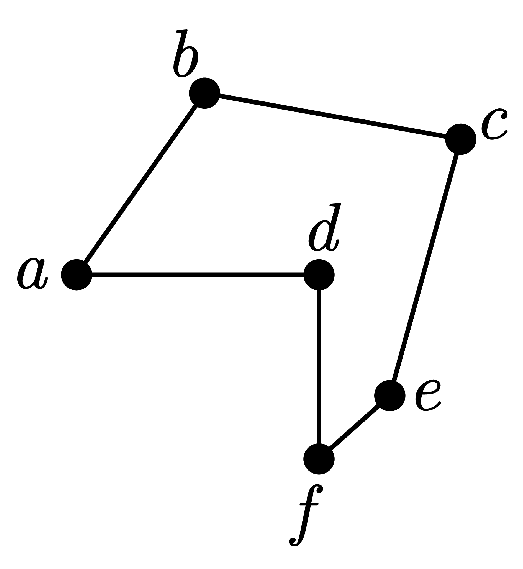
\includegraphics[width=.33\linewidth]{邻域结构-N1-Tour.pdf}}
    \subfloat[全局最优解$s^* \in \mathcal{N}_2 \in \mathcal{G}$ \label{subfig:邻域结构2-全局最优解}]{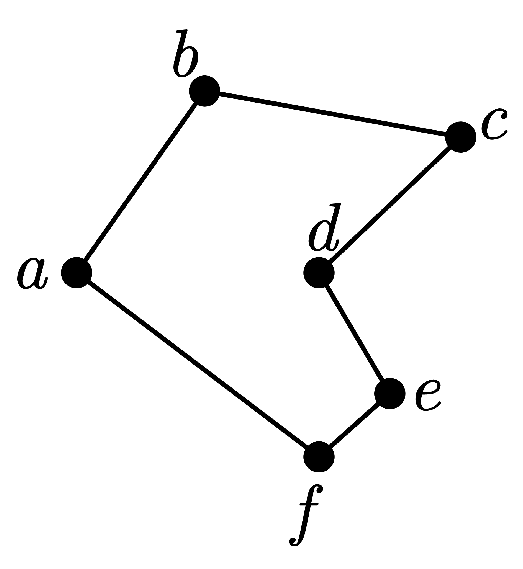
\includegraphics[width=.33\linewidth]{邻域结构-N2-Tour-Opt.pdf}}
    \caption[]{邻域结构示意图(续)}
\end{figure}
\par
如\autoref{fig:邻域结构示意图}~所示,给定一个TSP问题$\mathcal{P}$和问题$\mathcal{P}$的全连接图$\mathcal{G}$,由\autoref{def:邻域结构}~可知,当每个顶点的候选集由剩余所有顶点组成时,那么问题$\mathcal{P}$的邻域结构就是$\mathcal{G}$。在\autoref{fig:邻域结构示意图}~中,\autoref{subfig:全连接图}~就是一个全连接图。由算法\ref{alg:局部搜索算法框架}~可知,当邻域结构是全连接图时,这使得算法需要搜索整个搜索空间,显然不符合题意。因此,我们需要对邻域结构进行定制。如\autoref{subfig:邻域结构1}~所示,虽然\autoref{subfig:邻域结构1}~的邻域结构足够的小,但是,它并没有将\autoref{subfig:邻域结构2-全局最优解}~所示的最优路径中的所有边(如边$af$)都包含进去,当算法使用这个邻域结构,不用其他策略时,无论如何也不能搜索到最优解(只能搜索到局部最优解,如\autoref{subfig:邻域结构1-局部最优解})。所以,我们设计的邻域结构(如\autoref{subfig:邻域结构2})不仅要小,还需要保证足够的质量,以确保算法能够搜索到满意的解。
% 整图
% \begin{figure}[t]
%     \subfloat[全连接图$\mathcal{G}$ \label{subfig:全连接图}]{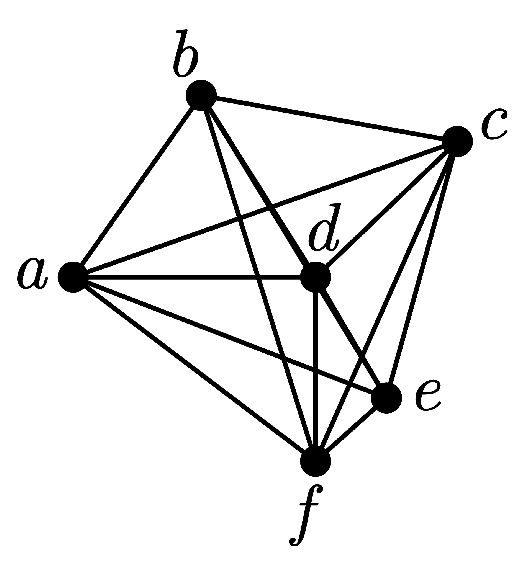
\includegraphics[width=.33\linewidth]{邻域结构-完全图.pdf}}
%     \subfloat[邻居结构$\mathcal{N}_1$ \label{subfig:邻域结构1}]{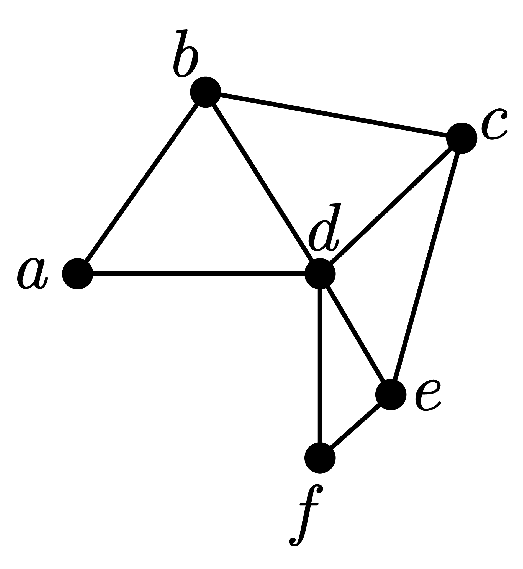
\includegraphics[width=.33\linewidth]{邻域结构-N1.pdf}}
%     \subfloat[邻居结构$\mathcal{N}_2$ \label{subfig:邻域结构2}]{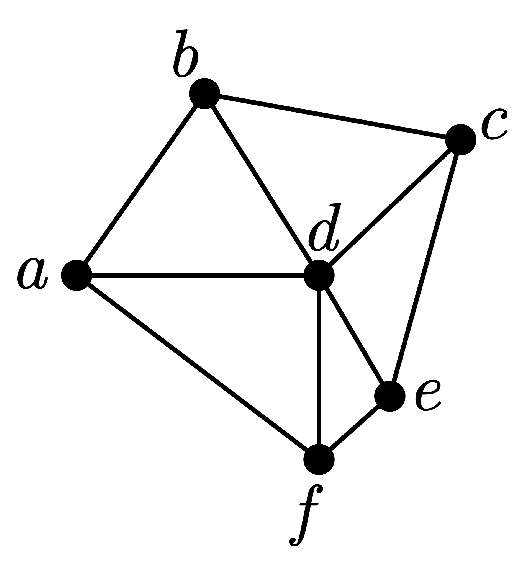
\includegraphics[width=.33\linewidth]{邻域结构-N2.pdf}} \\
%     \subfloat[局部最优解$s^* \in \mathcal{N}_1 \in \mathcal{G}$ \label{subfig:邻域结构1-局部最优解}]{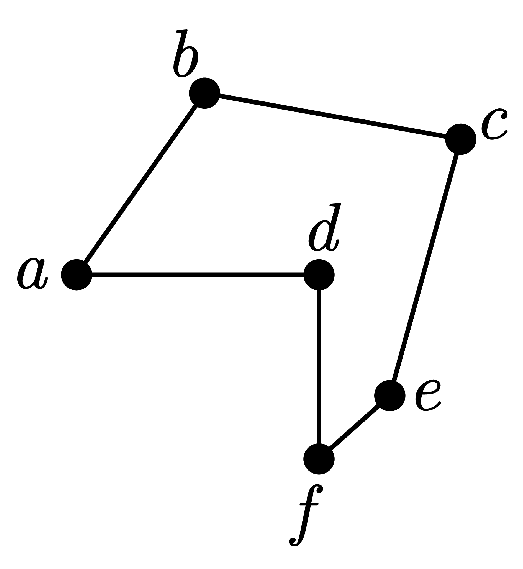
\includegraphics[width=.33\linewidth]{邻域结构-N1-Tour.pdf}}
%     \subfloat[全局最优解$s^* \in \mathcal{N}_2 \in \mathcal{G}$ \label{subfig:邻域结构2-局部最优解}]{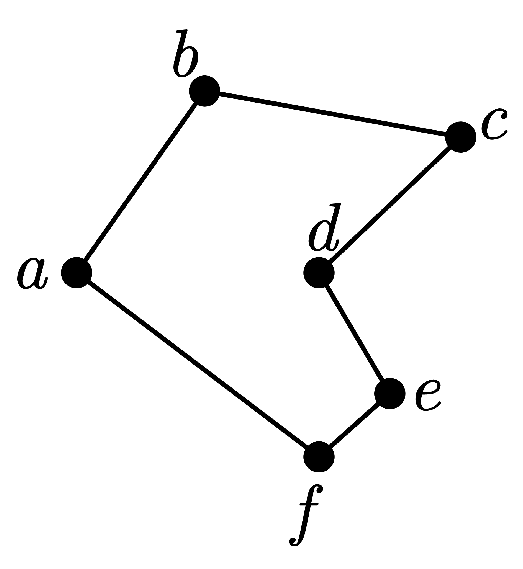
\includegraphics[width=.33\linewidth]{邻域结构-N2-Tour-Opt.pdf}}
%     \caption[邻域结构示意图]{邻域结构示意图}
%     \label{fig:邻域结构示意图}
% \end{figure}

\subsection{邻域动作}
\label{subsec:背景介绍:局部搜索:邻域动作}
由\autoref{def:邻域动作和邻域}~可知,邻域动作是一个函数,通过这个函数,算法能够在当前解的邻域中,生成对应的邻居解集合。由章节\ref{subsec:背景介绍:多目标组合优化算法:进化算法}~可知,遗传操作(交叉、变异算子)是进化算法中最重要的组件之一,它的作用就是产生新个体。又因为多目标组合优化问题的决策空间是离散且巨大的,这导致交叉、变异等算子生成新个体的效率和质量都达不到要求。因此,将邻域动作作为进化算法的一部分,替代遗传操作在算法中的功能,以局部搜索的思想来产生优质的子代个体。
\par
在组合优化问题中,邻域动作的规则不仅与问题的解的编码形式相关,更是在邻域结构的基础上来进行搜索产生新解的。因此,为保证与邻域的一致性,统一使用TSP和MOTSP。对于TSP问题,其解的编码形式为一个所有顶点组成的序列路径。针对序列路径,产生新个体的方式有很多。比如,有一序列路径$s = <v_1, v_2, v_3, v_4, v_5>$,任意交换两个顶点($v_2, v_3$)的位置\cite{borges1998basis}~,这样就在$s$的基础上,产生了一个$s$的邻居解$s' = <v_1, v_3, v_2, v_4, v_5>$。其中“交换两个顶点”这个动作就是邻域动作。
\par
\autoref{fig:k-opt示意图}~是一种名为k-opt的邻域动作规则\cite{helsgaun2006effective}~,其中k代表要交换的边数,k越大,代表新个体对原解的改动越大,并且,搜索所有解的判断时间也是k的指数倍。\autoref{subfig:2-opt}~中是2-opt移动示意图,原序列路径为$s=<v_1, v_2, v_4, v_3>$,在经由2-opt后,$s$删除$x_1, x_2$两条边,连接$y_1, y_2$两条边得到$s'=\{ v_1, v_4, v_2, v_3 \}$,相当于将$s$中的$x_1, x_2$两条边替换成$y_1, y_2$两条边,由此生成$s'$。同理,\autoref{subfig:3-opt}~为3-opt,\autoref{subfig:4-opt}~为4-opt。从图中很容易知道,一条序列路径$s$经由k-opt操作后,就是将$s$中的k条边,使用特定的交换策略,替换成不属于原序列路径的不同的k条边,这样就可以产生了$s'$。并且,从图中可以看出,k-opt是在(k-1)-opt的基础上再进行一次换边操作的,在使用k-opt时,我们期望k越大,获得的结果越好,并且对于足够大的k,我们期望序列路径$s$经由k-opt操作得到的$s'$应该是最优的。但是,随着k的增大,测试所有可能交换的边所需的操作次数增长得非常快。并且,我们并不知道给定问题到底需要设置多大的k才能获得可接受的优化结果,这也是使用k-opt算子无法避免的一个缺点。
\begin{figure}[htb]
    \subfloat[2-opt \label{subfig:2-opt}]{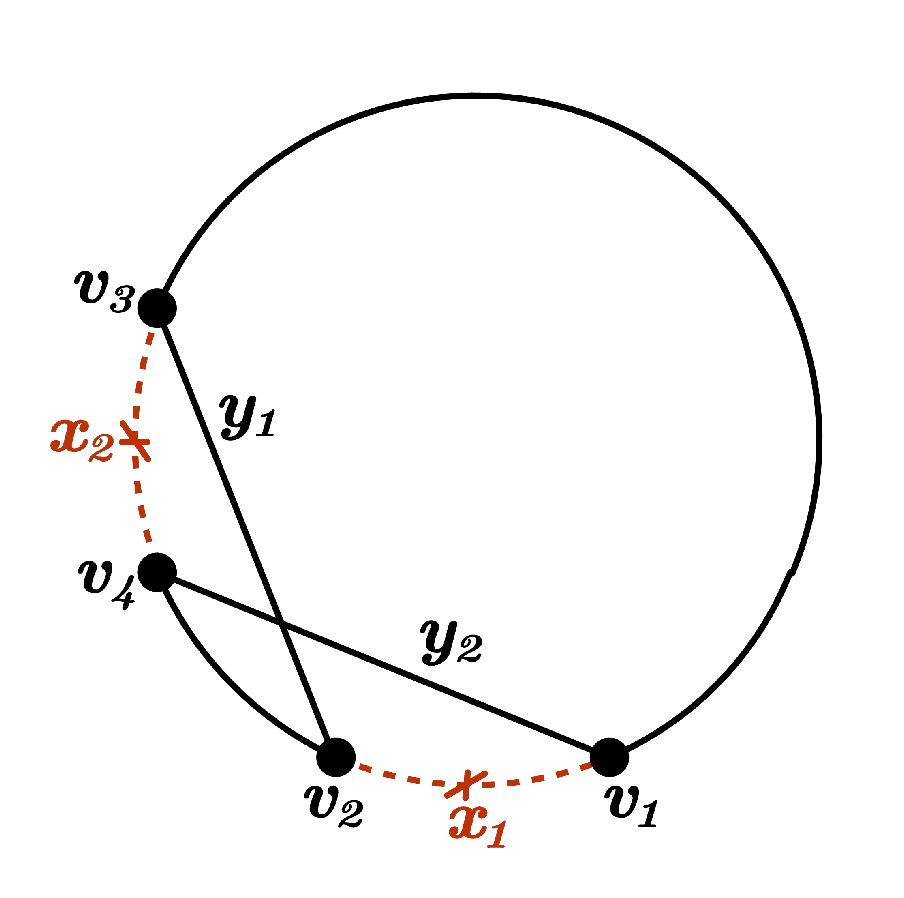
\includegraphics[width=.3\linewidth]{k-opt-2.pdf}}\quad
    \subfloat[3-opt \label{subfig:3-opt}]{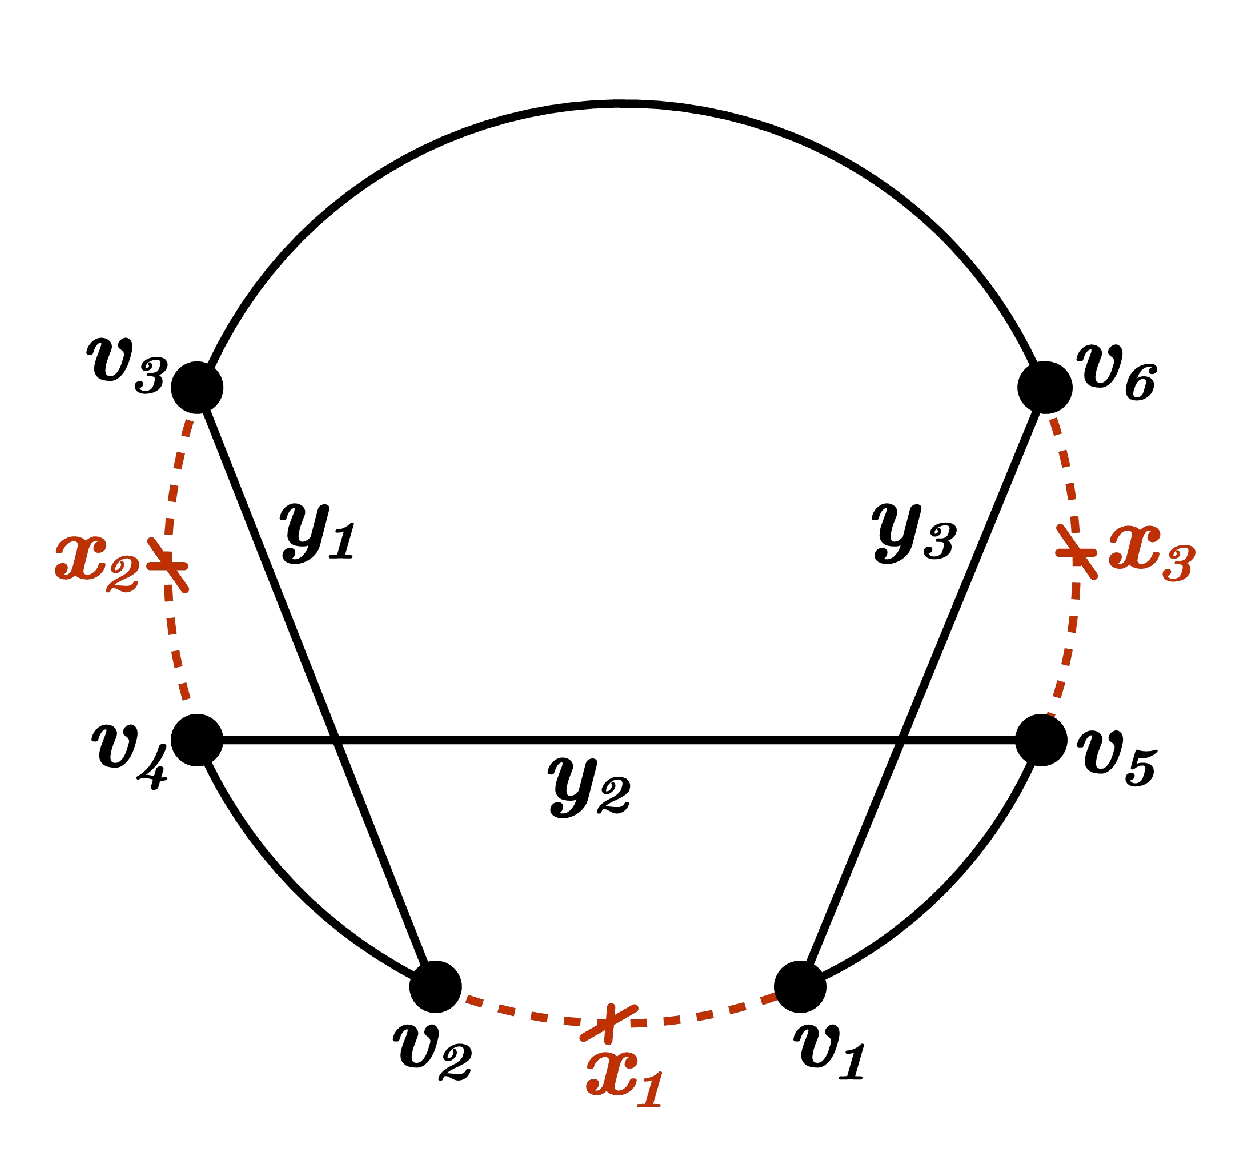
\includegraphics[width=.3\linewidth]{k-opt-3.pdf}}\quad
    \subfloat[4-opt \label{subfig:4-opt}]{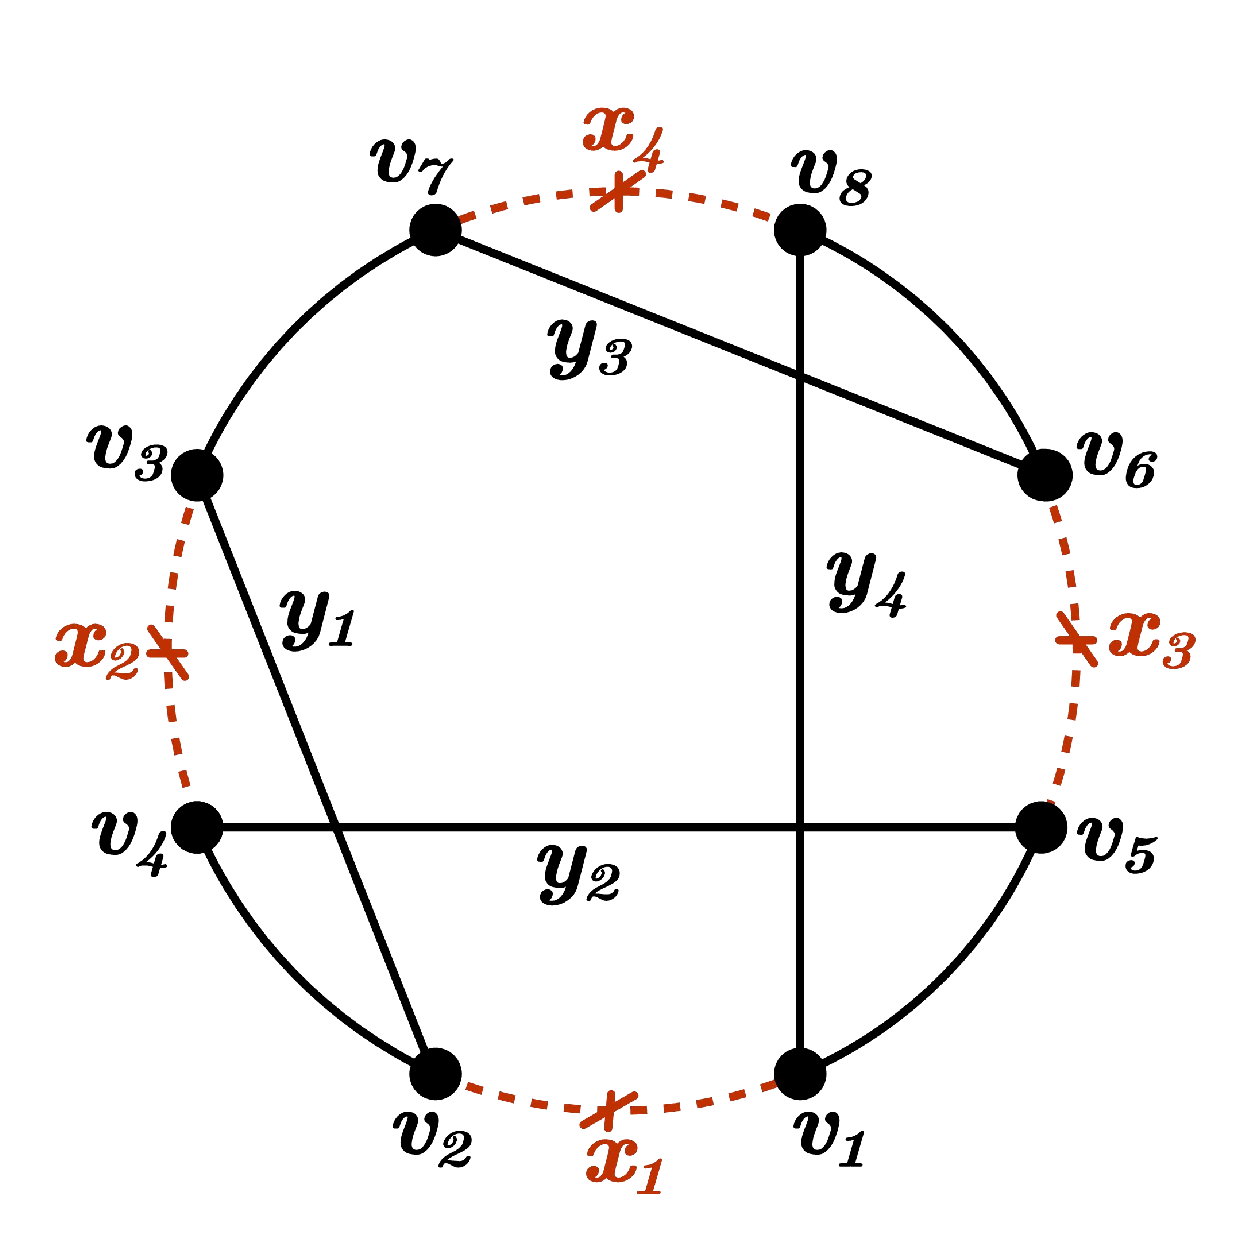
\includegraphics[width=.3\linewidth]{k-opt-4.pdf}}
    \caption[k-opt示意图]{k-opt示意图}
    \label{fig:k-opt示意图}
\end{figure}

% \subsection{Lin-Kernighan算法}
% \label{subsec:背景介绍:局部搜索:Lin-Kernighan算法}
% 针对上一节\ref{subsec:背景介绍:局部搜索:邻域动作}~中,k-opt算法无法确定k值这一缺点,Lin和Kernighan提出了一种补救措施:k-opt算法,k值可变,在执行过程中动态变化。该算法从考虑要交换的一组r=2链接开始,并在每个迭代步骤中决定是否应考虑一组r+1链接。该算法基于以下主要原则:
% \begin{itemize}
%     \item 使用顺序移动;
%     \item 必须选择要在序列中删除的最后一个链接,以便如果序列中没有更多步骤,则可以添加一个链接来结束游览(在每个步骤中,我们都可以停止并进行有效的移动);
%     \item 每个部分的收益总和必须是正的(移动必须是有希望的);
%     \item 删除的链接集和添加的链接集应该分开(一旦链接被删除,就不能再添加;一旦添加了链接,就不能删除;)。
% \end{itemize}

\section{进化迁移优化}
\label{sec:背景介绍:进化迁移优化}
迁移学习使用从源域(Source Domains,SD)中获取的知识来提升不同(但相关)目标域(Target Domains,TD)的学习能力\cite{pan2009survey}。相似地,进化迁移优化(Evolutionary Transfer Optimization,ETO)是一种将EA求解器与知识学习和跨领域信息转移相结合,以实现更好的优化效率和性能的范式。Kay在文中提到\cite{tan2021evolutionary},ETO虽然是一个兴起不久的优化范式,但是它已经在许多优化领域(比如:多任务优化、多目标优化和机器学习等)发挥了重要的作用。
\par
针对多目标优化问题来说,ETO旨在通过学习或迁移解、结构化信息等与问题相关的有用特征,在提高解的质量或搜索速度等方面来提高算法的性能。从算法设计的角度来说,现有的ETO方法可以分为同构(Homogenous)ETO和异构(Heterogeneous)ETO:
\begin{itemize}
    \item \textbf{同构ETO:}共享相同搜索空间的跨问题的知识迁移。
    \item \textbf{异构ETO:}跨具有不同搜索空间的问题之间的知识迁移。
\end{itemize}
此外,同构ETO已通过以不同子问题之间交换PS中解的形式实现跨子问题的知识迁移的方式应用于多目标和超多目标优化问题中\cite{tan2021evolutionary}。如\autoref{fig:跨问题知识迁移示意图}~所示,多目标和超多目标优化中的有用知识可以采用非支配解集、代理模型等形式来实现跨问题的知识迁移。如果ETO取得了在有知识迁移的情况下比没有知识迁移更好(更差)的表现,则称为正(负)迁移。
\begin{figure}[htb]
    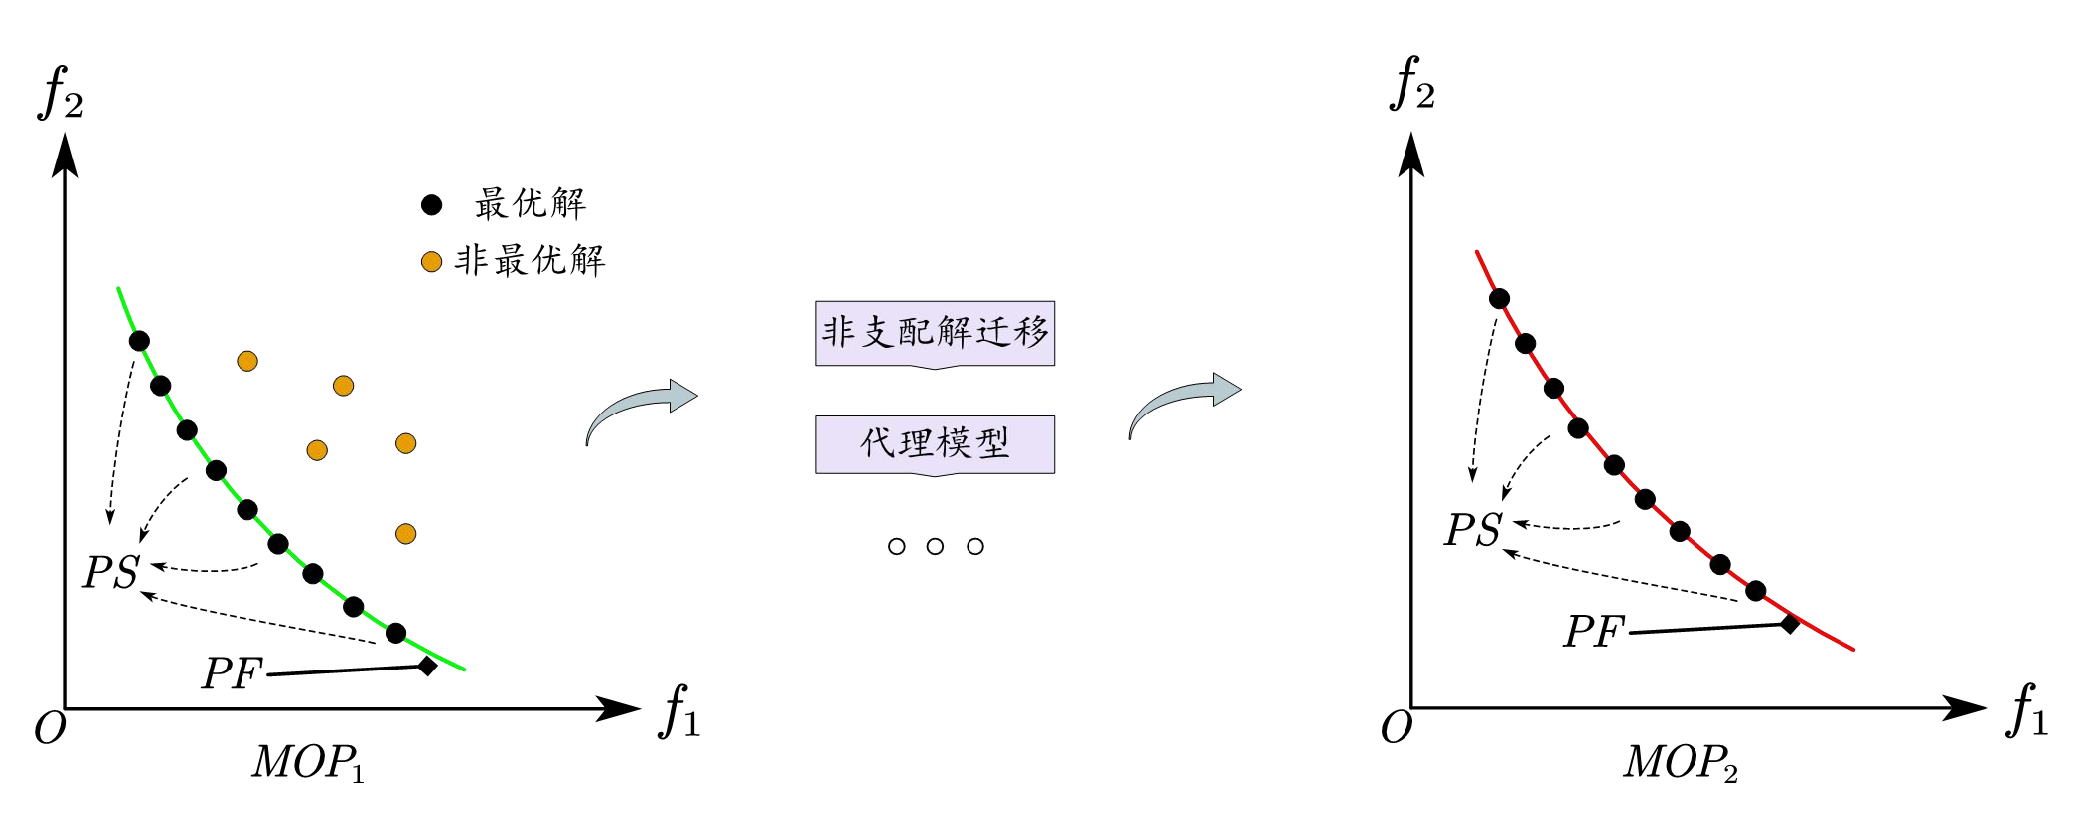
\includegraphics[width=\linewidth]{ETO.pdf}
    \caption[跨问题知识迁移示意图]{跨问题知识迁移示意图}
    \label{fig:跨问题知识迁移示意图}
\end{figure}
\par
直观地说,随着多目标优化问题中目标数量的增加,要迁移的非支配解的数量将急剧增加。因此,与只迁移MOP问题中非支配解的ETO相比,正确地构建源域和目标域中可迁移知识之间的映射关系是我们应该研究的重点。并且我们需要深入分析,在MOP中,什么信息是有用的,以及这些信息如何与跨问题域的多个目标相关连的。这可以更好地了解ETO在多目标和多目标优化中怎样并且在什么时候能够实现正迁移。

\section{性能评价指标}
\label{sec:背景介绍:性能评价指标}
对于一个算法,抛开其本身的复杂性而言,其表现好坏则是通过这个算法所求得相应问题的最终结果的优劣而定。对于CMOPs来说,其最终结果以非支配解集(NDSet,\autoref{def:非支配解集})的形式呈现。所以,一个MOEA的性能通常从两个方面进行评估:
\begin{enumerate}
    \item 群体解集的收敛性:NDSet与真实Pareto前沿(PF)的贴合程度。
    \item 群体解集的多样性:NDSet在空间上分布的均匀程度和广泛程度。
\end{enumerate}
\par
Knowles等人于2006年在文中\cite{knowles2006tutorial}介绍了很多评估NDSet性能的评价指标。例如:超体积度量指标(Hypervolume,HV)\cite{zitzler1999multiobjective}、反向世代距离指标(Inverted Generational Distance,IGD)\cite{czyzzak1998pareto}和集合覆盖度量指标(Set Converage,C-Metric)\cite{zitzler1999multiobjective}等。在本文中,除了需要对MOEA的性能进行评估外,还需要对邻域结构(最优边遗失率指标\cite{helsgaun2018using})和TSP问题的解进行质量评估(距离趋近度指标\cite{helsgaun2018using}),下面将分节详细介绍。

\subsection{超体积度量指标}
\label{subsec:背景介绍:性能评价指标:超体积度量指标}
超体积度量指标HV是一种通过计算参考点与NDSet围成空间的超体积实现对算法综合性能评价的方法,其数学形式如下:
\begin{align}
    \label{eq:HV}
    HV = \mathcal{L} (\bigcup_{i=1}^{|\mathcal{S}|} v_i).
\end{align}
其中,$\mathcal{L}$为Lebesgue测度,$\mathcal{S}$代表NDSet,$| \cdot  \vert $代表集合中元素的个数,$v_i$为非支配个体$s_i \in \mathcal{S}$和参考点$z^*$构成的超体积。
\begin{figure}[htb]
    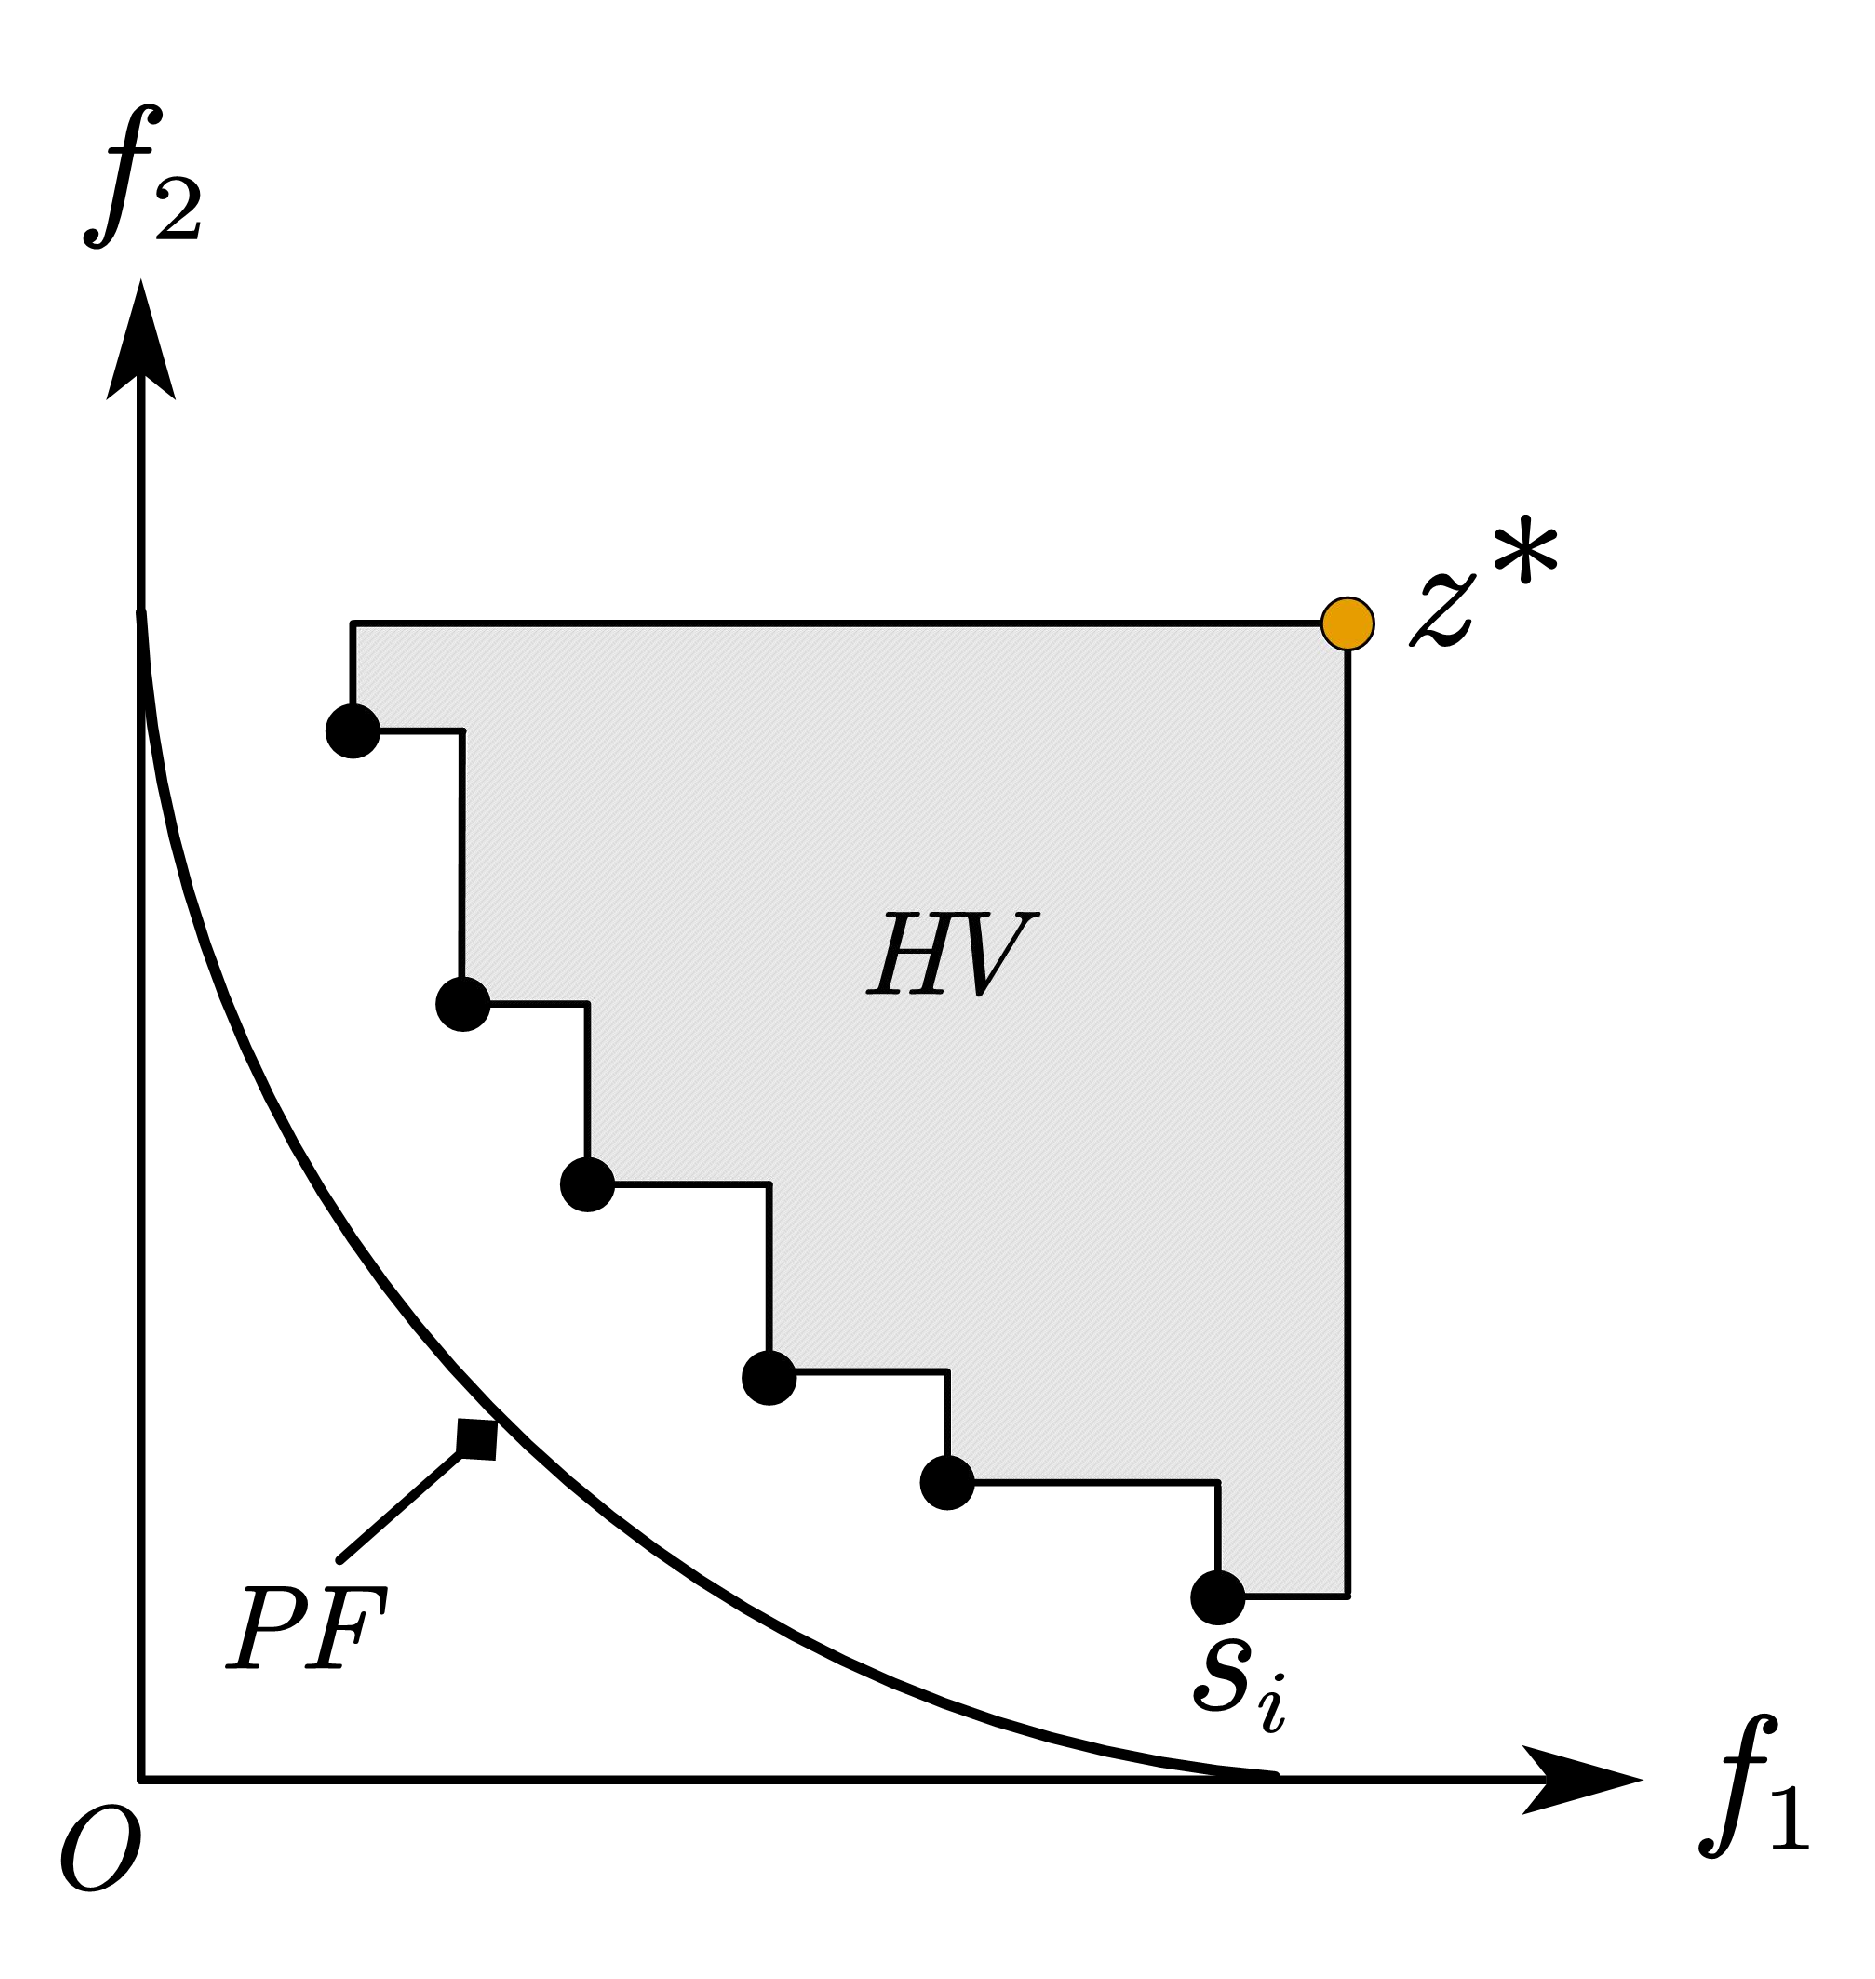
\includegraphics[width=.45\linewidth]{HV.pdf}
    \caption[HV指标示意图]{HV指标示意图}
    \label{fig:HV指标示意图}
\end{figure}
\par
如\autoref{fig:HV指标示意图}~所示是一个二目标问题的非支配解集的超体积度量示意图,其中超体积度量值为NDSet和参考点$z^*$构成的阴影区域的面积。$z^*$的选择方式有多种,常用的有:NDSet每维上的最大值组成的向量和松散形式的最差点\cite{deb2010toward}。从图中容易知道,HV指标值同样遵循Pareto支配(\autoref{def:Pareto支配})原则,以最小化MOP为例,如果个体$s_1 \prec s_2$,则$s_1$的HV度量值一定大于$s_2$,同理,可推广到两个解集之间的支配关系。并且,计算HV指标值时,真实PF不是必需的,所以HV指标具有更好的实用性。但是,计算HV指标的时间复杂度非常大,而且参考点的选择也会影响HV指标的正确性\cite{zheng2007mop}。

\subsection{反向世代距离指标}
\label{subsec:背景介绍:性能评价指标:反向世代距离指标}
反向世代距离指标IGD也是一种兼顾收敛性和多样性的综合评价指标。世代距离是指NDSet中所有个体到Pareto最优解集(PS)的平均距离,而反向世代距离则是PS中的个体到所求NDSet的平均距离。由此,其计算公式可表述如下:
\begin{align}
    \label{eq:IGD}
    IGD = \frac{1}{|PS|} \sum_{\mathbf{x}^* \in PS} \min_{s \in \mathcal{S}} \ \mathit{d}(\mathbf{x}^*, s).
\end{align}
其中,$PS$为Pareto最优解集(真实PF的真子集),$| \cdot  \vert $代表集合中元素的个数,$\mathcal{S}$为非支配解集,$\mathit{d}(\mathbf{x}^*, s)$代表个体$\mathbf{x}^*$与个体$s$的欧几里得距离。IGD值越小,说明算法的综合性能越好。
\begin{figure}[htb]
    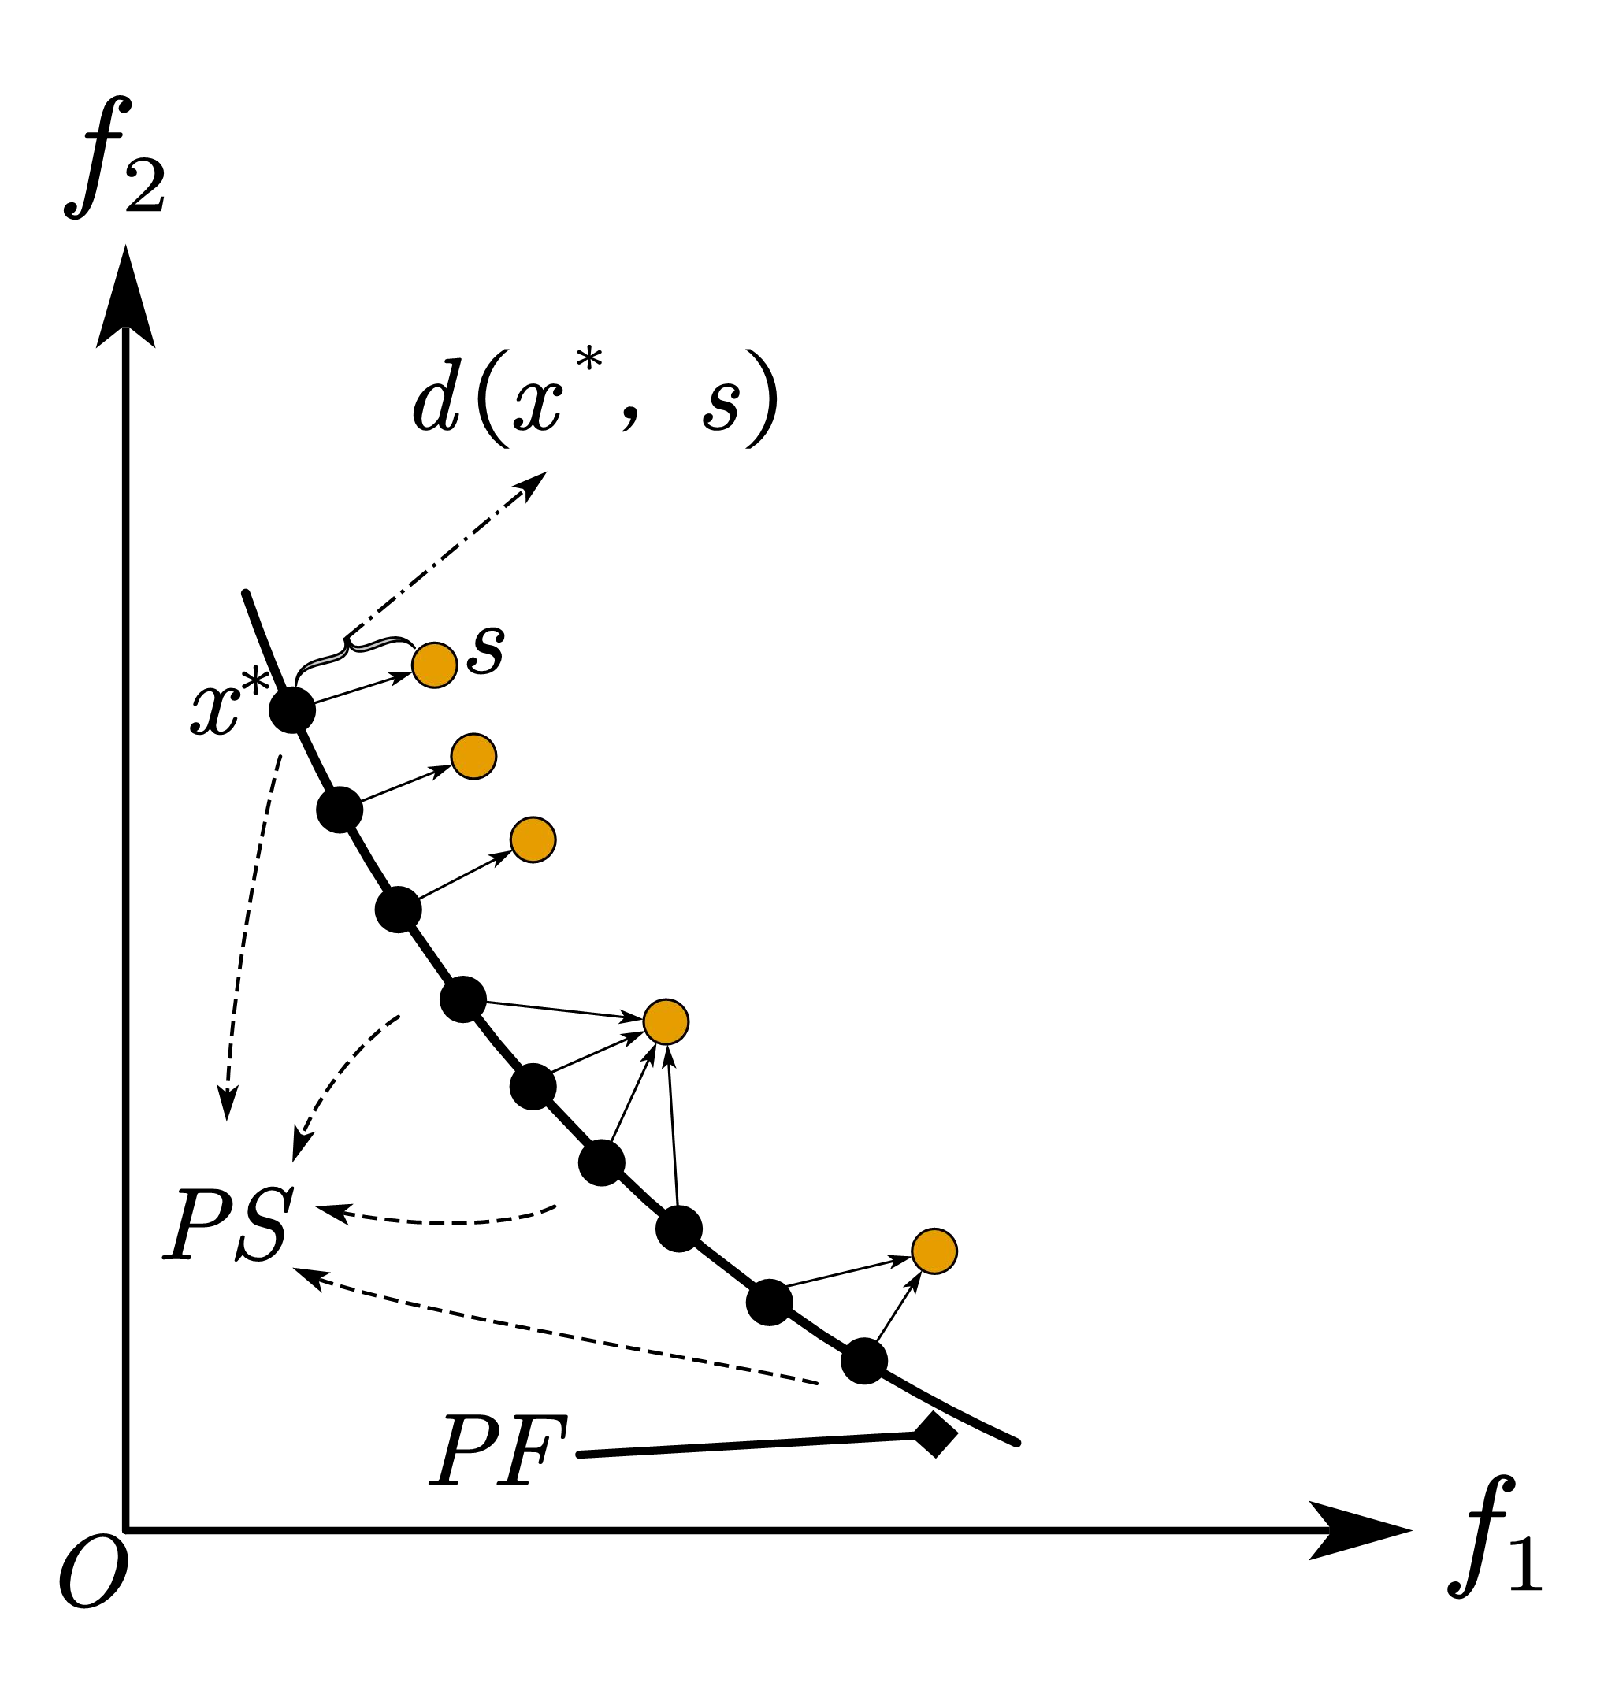
\includegraphics[width=.45\linewidth]{IGD.pdf}
    \caption[IGD指标示意图]{IGD指标示意图}
    \label{fig:IGD指标示意图}
\end{figure}
\par
此外,由\autoref{fig:IGD指标示意图}~可以直观地理解IGD指标对解集的综合性能评价。从图中可以看到,NDSet距离PF的距离远近能够直观地表现收敛性的好坏。同时,可以观察到,当NDSet的分布性不好时,由\autoref{eq:IGD}~计算可得IGD评价值会变大,并且在图中也可以看出,当NDSet分布均匀且广泛时,IGD评价值会很小。因此可以说明IGD评价指标不仅能够反映解集的收敛性,而且能够刻画解集的多样性(广泛且均匀)。但是,IGD指标需要通过真实PF来计算指标值,而现实问题大多都不知道其真实最优解,所以,这也成为其缺陷之一。

\subsection{集合覆盖度量指标}
\label{subsec:背景介绍:性能评价指标:集合覆盖度量指标}
集合覆盖度量指标C-Metric是一种两个解集相对覆盖率比较的方法,其利用解与解互相间的支配关系来判断两个解集之间的收敛性能的优劣。在C-Metric中,设在目标空间中有两个非支配解集$\mathcal{S}_a, \mathcal{S}_b \subseteq \mathcal{S}$,C-Metric则将($\mathcal{S}_a, \mathcal{S}_b$)映射到$[0, 1]$之间,得到$\mathcal{S}_a$与$\mathcal{S}_b$两解集之间的覆盖率,其数学形式如下:
\begin{align}
    \label{eq:C-Metric}
    C(\mathcal{S}_a, \mathcal{S}_b) = \frac{|\{ b \in B \ | \ \exists a \in A, a \prec b \}|}{|\mathcal{S}_b|} \times 100\%.
\end{align}
其中$| \cdot  \vert $代表集合中元素的个数,$C(\mathcal{S}_a, \mathcal{S}_b)$代表$\mathcal{S}_b$中所有能被$\mathcal{S}_a$中的解支配的解的数目占$\mathcal{S}_b$中解数目的百分比。
\par
由上述定义可知,如果$\mathcal{S}_a$中的解都弱支配$\mathcal{S}_b$中的解,那么C-Metric的值等于1,反之为0。一般的,由于$\mathcal{S}_a$和$\mathcal{S}_b$的交集并不为空,所以在评估解集的质量时,需要同时考虑$C(\mathcal{S}_a, \mathcal{S}_b)$和$C(\mathcal{S}_b, \mathcal{S}_a)$。要注意C-Metric方法并不是解集之间的距离上的比较,而是不同解集在支配关系上的相对比较。C-Metric的优点在于计算简单,但是计算复杂度取决于非支配排序算法,当目标数很大时,非支配排序算法的复杂度会很高,会耗费大量时间计算该指标。

\subsection{距离趋近度指标}
\label{subsec:背景介绍:性能评价指标:距离趋近度指标}
距离趋近度指标是一种用来评判单目标解质量的方法。对于最小化优化问题而言,距离趋近度指标利用解的适应值超过已知最优解的适应值的百分比来评判解的质量。假设有解$s$和最优解$s^*$,适应度函数$\varphi$,则其数学形式如下:
\begin{align}
    \label{eq:Gap}
    Gap = \frac{|\varphi (s) - \varphi (s^*)|}{\varphi (s^*)} \times 100\%.
\end{align}
其中$| \cdot  \vert $代表集合中元素的个数,一般地,我们很难知道具体问题的最优解,所以$s^*$一般可以用目前已知最优解来代替。
\par
由\autoref{eq:Gap}~可知,当适应度函数为线性函数时,其适应值就可以表现为解的值,当算法求得的解距离最优解越近,其Gap值就越小,代表该解质量越好。因此,可以利用距离趋近度指标来评估不同解的质量。

\subsection{最优边遗失率指标}
\label{subsec:背景介绍:性能评价指标:边遗失指标}
最优边遗失率指标是一种评估邻域结构质量的方法。对于图优化问题(如TSP、MST)而言,它们的解都是一个序列路径(节点之间可以构成边)构成。所以,最优边遗失率指标计算的是,邻域结构中,缺失的最优边(最优解中的边)的数目占最优解中边的数目的百分比。其数学描述如下:
\begin{align}
    \label{eq:Missing}
    Missing = (1 - \frac{|\{ e \ | \ e \in  \mathcal{E} (s^*) \bigcap \mathcal{E} (\mathcal{N}) \} |}{|\mathcal{E} (s^*)|}) \times 100\%.
\end{align}
其中$| \cdot  \vert $代表集合中元素的个数,$s^*$为最优解(一般用目前已知最优解替代),$\mathcal{N}$为邻域结构,$\mathcal{E} (\cdot)$获取解或者邻域结构中的边。
\par
由\autoref{eq:Missing}~可知,最优边遗失率指标仅能描述邻域结构的质量,并不能表示邻域结构的冗余度。当邻域结构是完全图(包含整个问题)时,那么它一定包含最优解中的所有边,Missing值为0,但这并不代表这个邻域结构是我们所期望的。所以,在用最优边遗失率指标对邻域结构进行评估时,应该建立在多个被评估的邻域结构拥有同样的稀疏度(出入度)的基础上。

\section{测试问题}
\label{sec:背景介绍:测试问题}
在本节中,将会介绍适用于本文的测试问题。由于本文提出了一种针对旅行商问题(Traveling Salesman Problem,TSP)的邻域结构生成的方法,为后续的基于邻域结构迁移的多目标进化算法提供一个可用于迁移的知识模型,所以,在本文将会用到单目标的TSP问题作为邻域结构生成的测试用例。又因为,邻域结构具有专属性(一种结构模型可能只适用于专属的问题),所以本文将使用多目标旅行商问题(Multi-Objective Traveling Salesman Problem,MOTSP)作为基于邻域结构迁移的多目标进化算法的测试用例。同时,在最后还会介绍多目标最小生成树问题( Multi-criteria Minimum Spanning Tree,MCMST),该问题具有和MOTSP类似的邻域结构,可以使用MOTSP的邻域结构尝试解决MCMST。本文提出的是解决具有图邻域结构组合优化问题的算法框架,有兴趣的读者可以尝试用该框架解决其他类型的多目标组合优化问题,介绍MCMST仅为读者提供思路启发。

\subsection{TSP}
\label{subsec:背景介绍:测试问题:TSP}
旅行商问题(TSP)是一种NP难的组合优化问题\cite{johnson1990traveling,baraglia2001hybrid,johnson2007experimental},最早于1959年Dantzig等人提出,并且在最优化领域中得到了深入的研究,同时许多优化方法都是用TSP作为一个测试基准。经典的TSP可以描述为:一个商品推销员想要去若干个城市推销商品,该推销员从其中一个城市出发,不重复的经过所有城市,最后回到出发地。推销员应该制定怎样的旅行路线,使得总行程最短。
\par
从图论的角度而言,TSP实质是在一个带权完全无向图中,找一个权值最小的哈密顿回路。该问题可抽象如下:给定一个完全图$\mathcal{G}=(V,E)$,其中$V = \{ v_1, \cdots, v_n \}$为包含$n$个元素的点集,$E = \{ e_{i,j} \ | \ v_i,v_j \in V, i \not = j \}$为包含$n^2-n$个元素的边集,寻找一条路径序列$\mathcal{T} = <t_1, \cdots, t_n>, t_i \in V $(所有点都被访问且仅访问一次)使得权重总和$f(\mathcal{T})$最小:
\begin{align}
    \label{eq:TSP}
    minimize \quad f(\mathcal{T}) = d(t_n,t_1) + \sum_{i=1}^{n-1} d(t_i,t_{i+1}).
\end{align}
其中,$d(v_i, v_j)$为边$e_{i,j}$的距离(权重)。

\subsection{MOTSP}
\label{subsec:背景介绍:测试问题:MOTSP}
多目标旅行商问题(MOTSP)相当于是TSP的一个扩展。TSP中,边权仅考虑了距离,所以在计算的时候只需要求总距离最短的路径序列。对于MOTSP而言,边权不仅只考虑距离,还会考虑旅行时间、费用等多种类型的权重,每多一种权重就相当于问题多了一个目标。所以,在求解MOTSP时,我们需要对多个权重(目标)进行权衡,从而给出一组非支配解作为MOTSP的解决方案。与TSP类似,MOTSP同样是选择一条路径序列$\mathcal{T} = <t_1, \cdots, t_n>, t_i \in V $,使得各目标权重总和最小,其数学描述如下:
\begin{align}
    \label{eq:MOTSP}
    minimize \quad f_k(\mathcal{T}) & = d_k(t_n,t_1) + \sum_{i=1}^{n-1} d_k(t_i,t_{i+1}), \\
    k & \in \{1, \cdots, m\}. \notag
\end{align}
其中,$d_k(v_i, v_j)$为边$e_{i,j}$第$k$个目标上的权重。
% MOTSP因其易于理解、模型简单等特点,被众多多目标组合优化算法用作基准测试问题\cite{cheng2012multi,shim2012hybridxia2017reference}。

\subsection{MCMST}
\label{subsec:背景介绍:测试问题:MCMST}
最小生成树(Minimum Spanning Tree,MST)问题是一个经典的组合优化问题,其目标是构造一个带全图的最小权值总和的生成树。设有一个带权无向图$\mathcal{G}=(V,E,W)$,其中$V = \{ v_1, \cdots, v_n \}$为点集,$E = \{ e_{i,j} \ | \ v_i,v_j \in V, i \not = j \}$为边集,$W = \{ w_{i,j} \ | \ e_{i,j} \in E, i \not = j \}$为边权集,寻找一个包含所有点的树$\mathcal{T} = (V, E_{\mathcal{T}}, W_\mathcal{T}), E_{\mathcal{T}} \subset E,W_\mathcal{T} \subset W$,使得$W_\mathcal{T}$最小,则称$\mathcal{T}$为图$\mathcal{G}$的最小生成树。
\par
与MOTSP类似,当考虑多种类型的权重时,该问题就是一个多目标最小生成树(Multi-criteria Minimum Spanning Tree,MCMST)问题。所以,MCMST的解同样为一组非支配解,其中每个解都是一个最小生成树的边集$E_{\mathcal{T}}$,则其数学描述如下:
\begin{align}
    \label{eq:MCMST}
    minimize \quad f_k(\mathcal{T}) & = \sum_{e_{i,j} \in E_{\mathcal{T}}} w_{i,j}^k, \\
    k & \in \{1, \cdots, m\}. \notag
\end{align}
其中,$w_{i,j}^k$为边$e_{i,j}$第$k$个目标上的权重。容易知道解$\mathcal{T}$中包含$n$个顶点,$n-1$条边。

\section{本章小结}
\label{sec:背景介绍:本章小结}
本章的主要目的是为后续章节提供一定的基础理论支撑。本章在一开始就介绍了多目标优化问题的定义及相关概念,并由此对多目标进化的基础算法进行了简要的介绍,同时详细介绍了基于分解的多目标进化算法。然后针对进化算法在组合优化中遗传算子效率的问题,引出了在基于分解的多目标进化算法中使用局部搜索来对多目标组合优化问题进行优化的思想。接着介绍了与其他领域相结合的进化迁移优化相关概念。最后,介绍了一些性能评价指标和经典的测试问题。
\chapter{基于最小生成树和欧拉回路的邻域结构生成方法}
\label{chap:NS_Method}

\section{引言}
\label{sec:NS_Method:引言}
% 需要用LS中的NS,从何而来,为什么用,如何用,最终结果如何?
Fourman等人于1985年在解决多目标优化问题时提出多目标进化算法(MOEA)\cite{fourman1985compaction,schaffer1985multiple},其实质就是进化算法(EA)在多目标优化领域的一种扩展。由章节~\ref{sec:背景介绍:多目标组合优化算法}~介绍可知,EA是一种受达尔文进化论启发而产生的、基于种群且不断迭代进化的一大类元启发式算法,其中进化规则中的遗传操作正是EA的核心部分。EA通过模拟自然界物种适者生存、优胜劣汰的遗传机制,从而使得种群在表现出基因多样性的同时相互竞争,以致整个种群得以进化。而遗传机制其中一个特征就是,通过复制、交叉、变异操作从父代种群个体的基因特征中产生新的子代个体。然而对于大多数多目标组合优化问题而言,其决策空间(基因编码形式)是离散并十分巨大的,导致了这些遗传操作(复制、交叉、变异算子等)生成子代个体的基因特征变化不大,生成新个体的质量和效率都会大大降低,从而使得种群的进化较为缓慢。因此,我们需要采用一些策略或算法来替代遗传操作的部分甚至全部功能,嵌入到多目标进化算法当中,从而改善生成新个体质量和效率低的问题。
\par
通过章节~\ref{sec:背景介绍:局部搜索}~的介绍可知,局部搜索算子是能够改善甚至替代多目标进化算法中遗传操作来生成新个体的方法之一。对于一个组合优化问题而言,局部搜索算子就是在该问题的候选解空间上进行搜索的一种方法,它依赖邻域结构来生成高质量的邻居解(新个体),这正是遗传操作的特征之一。而邻域结构正是局部搜索算法中最核心的部分之一。一个质量好的邻域结构,不仅能够能够帮助局部搜索算子搜索到高质量的解,而且能够加速整个算法的运行速度,使得MOEA收敛得更好且更快。比如,Lust等人\cite{lust2010speed}采用非支配排序的方式为二目标TSP问题构建了一个稀疏图(邻域结构),从而加速2PPLS\cite{lust2010two}算法求解该问题的运行速度。并且,LKH(Lin Kernighan Helsgaun)\cite{helsgaun2000effective}是目前求解TSP问题最有效的方法之一,其在算法中也用到了名为$\alpha$-nearest\cite{held1970traveling,held1971traveling}的方法生成的邻域结构,使用该邻域结构的LKH不仅提高了算法整体的运行效率,同时,算法中更是采用了一些特殊的规则与邻域结构相配合,使得算法能够快速得搜索到高质量的候选解。这些足以说明邻域结构在算法中能够发挥的作用。
\par
邻域结构除了能够作为局部搜索算子的一部分,还能够表征对应问题的内在信息被用来在不同域(SD,TD)中迁移的知识。由章节~\ref{sec:背景介绍:进化迁移优化}~可知,在MOPs中,目前进化迁移优化(ETO)都是将目标空间的解(非支配解,非最优解)当作被迁移的知识。在本文中,我们将邻域结构当作被迁移的知识,提出一种基于邻域结构迁移的多目标组合优化算法。
\par
然而,邻域结构的构建与我们所要解决的问题紧密相关。邻域结构展现的形式需要我们对具体的组合优化问题有深刻的理解,并且能将该问题的内在信息用某种结构表示出来。这也正是我们所言研究的重点。我们将通过本章节对TSP问题的邻域结构的生成方法进行详细地介绍,并期望研究者能够从该工作中得到启发,设计出更具泛化性(适用于多种组合优化问题)的邻域结构。

\section{研究动机}
\label{sec:NS_Method:研究动机}
% 现在研究的工作,现有工作的缺点和能够借鉴的地方,我的工作
% 为大型TSP实例构造一个每个点只有若干候选点的高质量的稀疏图是很有必要的
% 现有的构造邻域结构的方法复杂度过高,当问题规模变大或者为多目标问题(子问题变多,每个子问题都需要求相应的邻域结构,这就要求我们生成邻域结构的方法的时间复杂度要尽可能的低)构造邻域结构时,需要一个低于二次方时间复杂度的构造方法。k-NN,alpha-nearest等都是二次方时间复杂度的算法
由上一节的介绍可知,邻域结构不仅可以服务于局部搜索算子,从而产生高质量的子代个体并且对整个优化算法进行加速,而且还能够作为ETO中被用来迁移的知识信息。我们知道,针对不同的组合优化问题,其邻域结构的形式就可能不同,这就导致其构建方法也会不同。因此,在本文中,我们是在TSP问题和MOTSP问题的基础上提出的邻域结构生成方法。
\par
经由章节~\ref{sec:背景介绍:测试问题}~可知,TSP问题可以转化为在一个完全图$\mathcal{G} = (V,E)$中寻找一条总路径和最小的哈密顿回路。当完全图$\mathcal{G}$包含的点较少时,算法可以采用暴力的方式,每次将所有点都计算一遍,从而遍历获得问题的最优解。但是当完全图$\mathcal{G}$中包含的点较多时,暴力遍历的方式就会导致算法无法在期望时间内获得优质解。因此,要使得算法能够在短时间内搜索到优质解,一个关键的点就是为这个完全图$\mathcal{G}$构建一个每个点仅连接若干个点的子图(邻域结构)$\mathcal{N} \subseteq \mathcal{G}$。当邻域结构$\mathcal{N}$足够稀疏时,此时就算采用遍历的方式,也能够比用完全图作为邻域结构低一个数量级的时间复杂度获取到优质解。对于TSP问题,已经有一些方法来生成相应的稀疏网络。如,对于二维的欧几里得距离TSP实例,可以使用三角剖分(Delaunay\cite{krasnogor1995new})以$O(nlogn)$的时间复杂度构建一个稀疏图,其中$n$为顶点个数。当顶点的坐标为$r$维时,可以使用KD树\cite{bentley1975multidimensional}以$O(rnlogn)$的时间复杂度在点的每个象限中仅保留若干个最近的点,确保构建一个连接且稀疏的网络。但是,这两种方法都有明显的局限性,在TSP求解器LKH\cite{helsgaun2000effective,helsgaun2009general}中,Delaunay只能为二维坐标实例生成邻域结构,而KD树需要所有点的$r$维坐标。对于其他一般的情况,可以使用K最邻近(K-Nearest Neighbor,KNN)以$O(Kn^2)$的时间复杂度构建一个每个点只与最邻近的$K$个点相连的稀疏图。我们还常使用基于最小生成1-tree\cite{held1970traveling,held1971traveling}的$\alpha$-nearest来计算每个点所有边的$\alpha$评估值,其中$\alpha$值越小说明该边属于最优解的概率就越大,然后类似于KNN,选择$K$个$\alpha$最邻近的点来构建一个稀疏图。
\par
一般而言,使用$\alpha$-nearest生成邻域结构要比使用KNN生成的邻域结构质量上要好很多,虽然这两个都是二次方时间复杂度的算法。其原因一是$\alpha$-nearest使用最小生成1-tree(定义3.1)来对边进行重评估,二是最终使用的最小生成1-tree是经过次梯度优化(算法3.1)得来的。次梯度优化作为$\alpha$-nearest的一个前置算法,可以提升最终生成邻域结构的质量,但是,算法在中间过程会产生大量未被使用的最小生成树(MST,算法只使用最终优化的MST),后续的算法也未使用这些MST。 
\par
综上所述,这些构建邻域结构算法除了对问题的类型有特殊要求外,其复杂度仍然过高($O(n^2)$),难以在大规模问题或者多目标超多子问题上使用。基于以上原因,我们就利用在次梯度优化中未被充分使用的众多MST,并且结合欧拉回路的构造巡回路径(解)的方法,提出了一种时间复杂度低于$O(n^2)$的、基于最小生成树和欧拉回路的邻域结构生成方法。

\section{相关定义与基本概念}
\label{sec:NS_Method:相关定义与基本概念}
在这一节中,将介绍一些有关邻域结构生成方法的基本概念,最小生成1-tree和欧拉回路的相关定义以及次梯度优化产生MST的过程。

\subsection{最小生成1-tree}
\label{subsec:NS_Method:相关定义与基本概念:最小生成1-tree}
在正式介绍最小生成1-tree(Minimum Spanning 1-tree,1MST)之前,我们需要先了解一些图论中的基本定义。设有一个无向加权图$\mathcal{G} = (V, E, W)$,其中$V = \{ v_1, \cdots, v_n \}$是包含$n$个元素的点集,$E = \{ e_{i,j} = (v_i,v_j) \ | \ v_i,v_j \in V, i \not = j \}$是边集,$W = \{ w_{i,j} \ | \ e_{i,j} \in E, i \not = j\} $为边权集。给定图$\mathcal{G}$一个边序列
\begin{align}
    \label{eq:边序列}
    \mathcal{E} \ & = \ <e_{1,2}, e_{2,3}, \cdots, e_{k-1,k}>, \\
    s.t. \quad & e_{i,i+1} = (v_i, v_{i+1}) \in E, \notag  \\
    & v_i, v_{i+1} \in V. \notag 
\end{align}
\begin{definition}[简单通路]
    \label{def:Path}
    边序列$\mathcal{E}$中有$i \in \{ 1, \dots, k-1 \}$,若所有边互不相同,则称边序列$\mathcal{E}$为点$v_1$到点$v_k$的简单通路,否则称为复杂通路。若简单通路中所有点互不相同,则称该简单通路为基本通路。在本文中,简单通路即基本通路,可简称为通路(\emph{\textbf{Path}})。
\end{definition}
\begin{definition}[简单回路]
    \label{def:Cycle}
    边序列$\mathcal{E}$中有$i \in \{ 1, \dots, k \}$,且$v_1=v_{k+1}$,若所有边互不相同,则称边序列$\mathcal{E}$为简单回路,否则称为复杂回路。若简单回路中除去$v_1=v_{k+1}$外所有点互不相同,则称该简单回路为基本回路。在本文中,简单回路即基本回路,可简称为回路(\emph{\textbf{Cycle}})。
\end{definition}
\begin{definition}[哈密顿回路]
    \label{def:Hamiltonian Cycle}
    若图$\mathcal{G}$存在回路$\mathcal{E}$(\autoref{def:Cycle}),且$k=n$,则称回路$\mathcal{E}$为哈密顿回路(\emph{\textbf{Hamiltonian Cycle}}),可简称为巡回路径(\emph{\textbf{Tour}})。
\end{definition}
\begin{definition}[连通图]
    \label{def:Connected Graph}
    在无向图$\mathcal{G}$中,对任意两个点$v_i, v_j \in V, i \not = j$存在通路(可称$v_i$和$v_j$连通(\emph{\textbf{Connected}}))(\autoref{def:Path}),则称图$\mathcal{G}$为连通图。
\end{definition}
\begin{definition}[树]
    \label{def:Tree}
    一个无回路(\autoref{def:Cycle})的连通图(\autoref{def:Connected Graph})是树(\emph{\textbf{Tree}})。
\end{definition}
\begin{definition}[生成树]
    \label{def:Spanning Tree}
    在无向图$\mathcal{G}$中,由点集$V$构成的一棵树(\autoref{def:Tree}),称为图$\mathcal{G}$的生成树。
\end{definition}
\begin{definition}[最小生成树]
    \label{def:Minimum Spanning Tree}
    在无向加权图$\mathcal{G}$中,所有边权和最小的生成树(\autoref{def:Spanning Tree}),称为图$\mathcal{G}$的最小生成树(Minimum Spanning Tree,\emph{\textbf{MST}})。
\end{definition}
\begin{definition}[生成1-tree]
    \label{def:Spanning 1-Tree}
    在无向加权图$\mathcal{G}$中,由点集$V/\{v_1\}$构成的生成树中的两个点,与$v_1$相连的图,称为生成1-tree。
\end{definition}
\par
从\autoref{def:Spanning 1-Tree}~和\autoref{fig:生成1-tree示意图}~可知,点$v_1$是可以任意选择的,并且生成1-tree并不是一颗树,而是一个特殊的连通图,因为生成1-tree包含一个回路。
\begin{figure}[htb]
    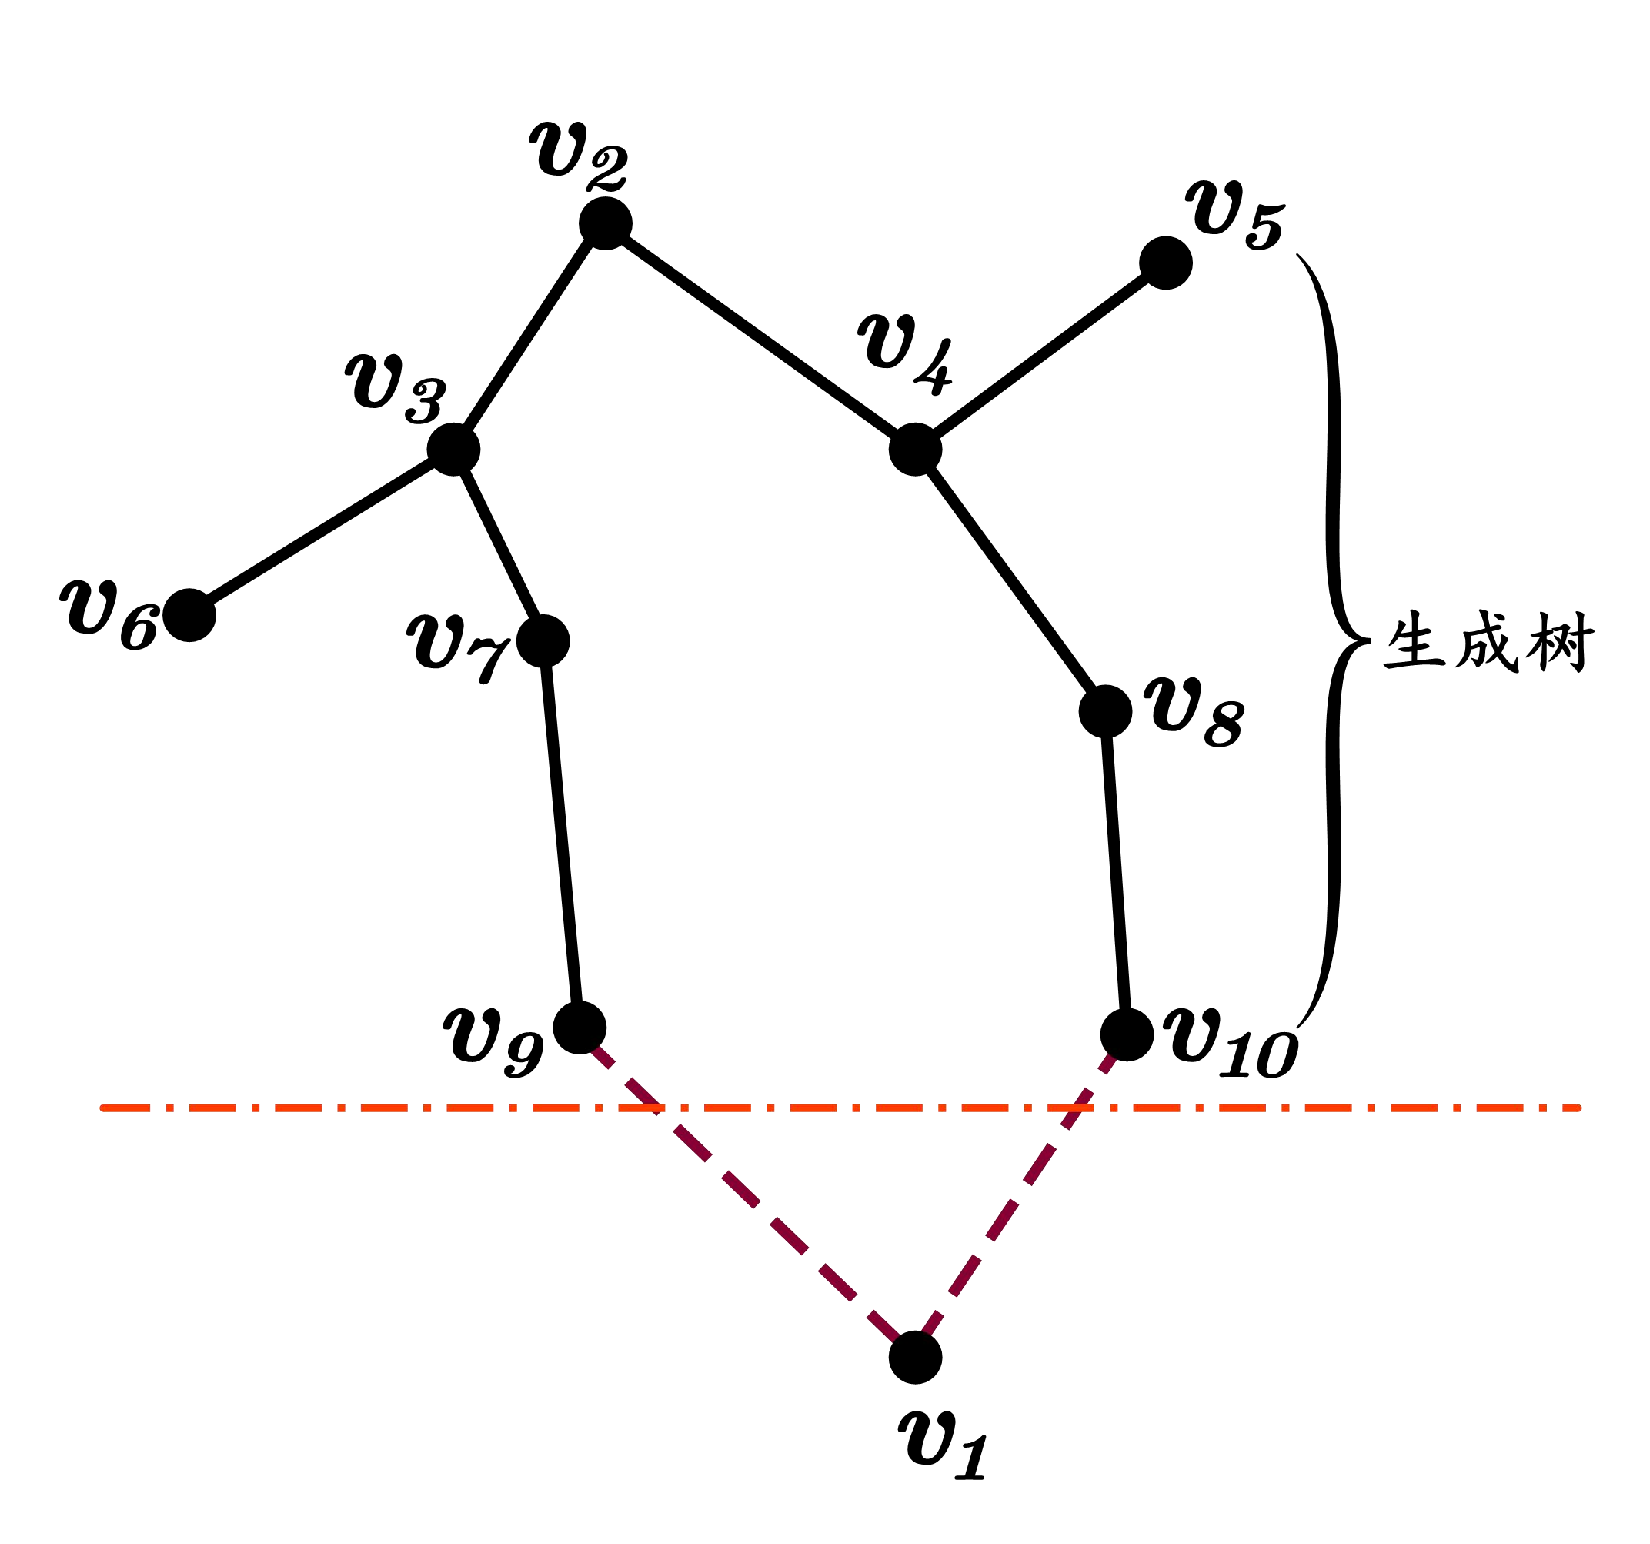
\includegraphics[width=.45\linewidth]{生成1-tree.pdf}
    \caption[生成1-tree示意图]{生成1-tree示意图 \\ 红虚线上方的是一颗不包含点$v_1$的生成树。点$v_1$通过两条边($e_{1,9}, e_{1,10}$)连接到生成树上。其中点$v_1$是任意的。图中生成1-tree包含一个回路$<e_{2,3}, e_{3,7}, e_{7,9}, e_{9,1}, e_{1,10}, e_{10,8}, e_{8,4}, e_{4,2}>$}
    \label{fig:生成1-tree示意图}
\end{figure}
\begin{definition}[最小生成1-tree]
    \label{def:Minimum Spanning 1-tree}
    在无向加权图$\mathcal{G}$中,所有边权和最小的生成1-tree(\autoref{def:Spanning 1-Tree}),称为图$\mathcal{G}$的最小生成1-tree(Minimum Spanning 1-tree,\emph{\textbf{1MST}})。
\end{definition}
\begin{definition}[点度]
    \label{def:Degree}
    顶点的度(\emph{\textbf{Degree}}),即该顶点所连接的边的数量。    
\end{definition}
\par
由哈密顿回路(巡回路径)(\autoref{def:Hamiltonian Cycle}),点度(\autoref{def:Degree})和最小生成1-tree(\autoref{def:Minimum Spanning 1-tree})等定义,可以得到以下推论:
\begin{corollary}
    \label{cor:Optimal Tour1}
    最优巡回路径(\autoref{def:Hamiltonian Cycle})是每个点度(\autoref{def:Degree})为2的最小生成1-tree(\autoref{def:Minimum Spanning 1-tree})。
\end{corollary}
\begin{corollary}
    \label{cor:Optimal Tour2}
    如果一个最小生成1-tree(\autoref{def:Minimum Spanning 1-tree})是巡回路径(\autoref{def:Hamiltonian Cycle}),则该巡回路径是最优的。
\end{corollary}
\par
由上述推论可以知道,TSP问题的最优解就是一个所有点度为2的1MST。但是,1MST一般是不规整的(点度不都为2),即便这样,一个不规整的1MST也会包含大量与最优巡回路径相同的边。而我们构造邻域结构的目的,就是为了在稀疏化图的同时,尽可能的包含这些可能在最优巡回路径中的边。因此,由1MST来构造的邻域结构具有更好的质量。


\subsection{欧拉回路}
\label{subsec:NS_Method:相关定义与基本概念:欧拉回路}
在图论中,欧拉路径(Eulerian Path)是连通图中的一条路径,它只访问图中的边一次(允许重复访问同一个顶点),且访问的起始点和终点不同。当访问的起始点和终点相同时,这条路径即为欧拉回路(Eulerian Cycle)。1736年,Leonhard Euler在解决著名的七桥问题时首次讨论了它们\cite{barnett2005early}。下面,将详细介绍与欧拉回路相关的定义和基本概念。
\begin{definition}[欧拉路径]
    \label{def:Eulerian Path}
    遍历连通图的每条边一次且仅一次,并且有不同的起始点和终点的路径,称为欧拉路径(\emph{\textbf{Eulerian Path}})。
\end{definition}  
\begin{definition}[欧拉回路]
    \label{def:Eulerian Cycle}
    欧拉回路(\emph{\textbf{Eulerian Cycle}})是起始点和终点相同的欧拉路径(\autoref{def:Eulerian Path})。
\end{definition}  
\begin{figure}[htb]
    \subfloat[无向连通图 \label{subfig:无向连通图1}]{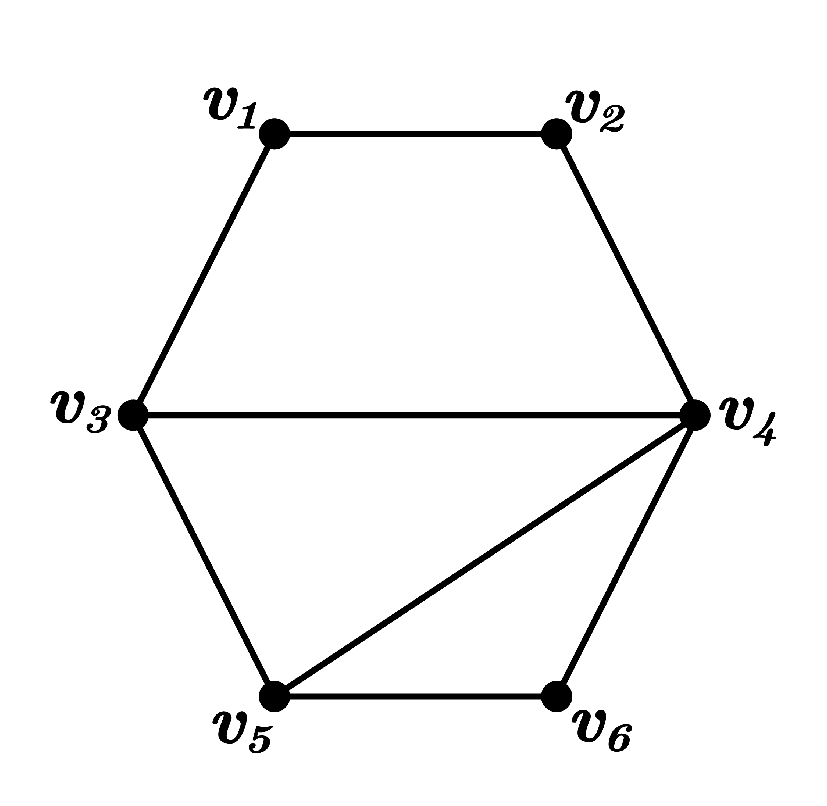
\includegraphics[width=.4\linewidth]{Euler Path Graph.pdf}}\quad
    \subfloat[欧拉路径 \label{subfig:欧拉路径}]{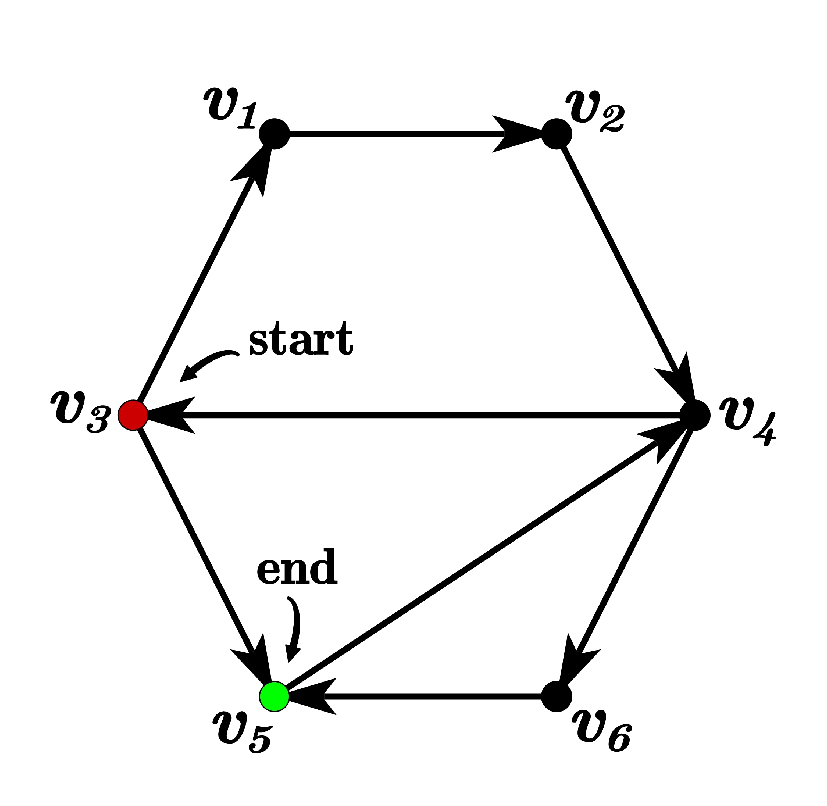
\includegraphics[width=.4\linewidth]{Euler Path.pdf}}
    \caption[欧拉路径示意图]{欧拉路径示意图 \\ 子图\subref{subfig:无向连通图1}~是无向连通图,子图\subref{subfig:欧拉路径}~是子图\subref{subfig:无向连通图1}~的一条欧拉路径$<v_3, v_1, v_2, v_4, v_3, v_5, v_4, v_6, v_5>$}
    \label{fig:欧拉路径示意图}
\end{figure}
\par
如\autoref{fig:欧拉路径示意图}~所示,\autoref{subfig:欧拉路径}~中的欧拉路径是\autoref{subfig:无向连通图1}~中无向连通图的其中一条欧拉路径,这条欧拉路径通过每条边一次,并且在不同的顶点开始($v_3$)和结束($v_5$)。但是,\autoref{subfig:无向连通图1}~中不存在欧拉回路,因为不存在起始点和终点相同的欧拉路径。
\begin{figure}[htb]
    \subfloat[无向连通图 \label{subfig:无向连通图2}]{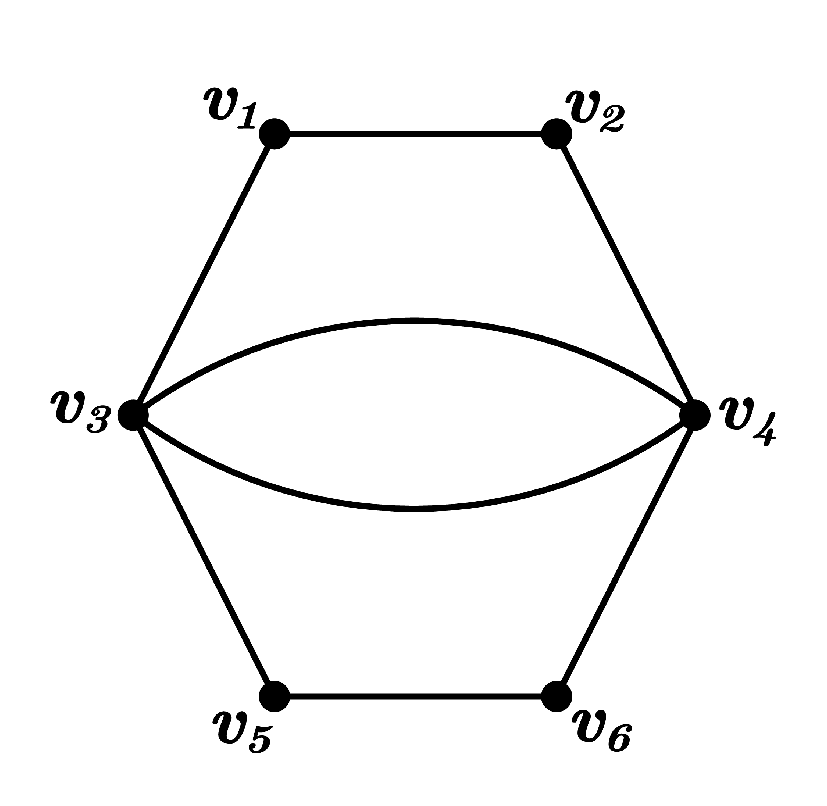
\includegraphics[width=.4\linewidth]{Euler Circuit Graph.pdf}}\quad
    \subfloat[欧拉回路 \label{subfig:欧拉回路}]{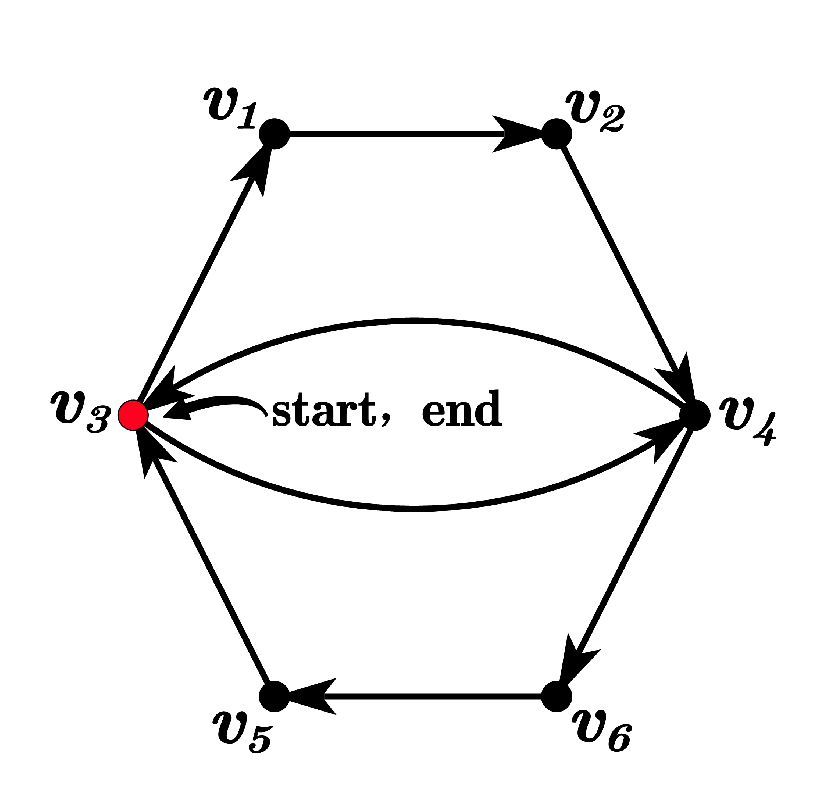
\includegraphics[width=.4\linewidth]{Euler Circuit.pdf}}
    \caption[欧拉回路示意图]{欧拉回路示意图 \\ 子图\subref{subfig:无向连通图2}~是无向连通图,子图\subref{subfig:欧拉回路}~是子图\subref{subfig:无向连通图2}~的一条欧拉回路$<v_3, v_1, v_2, v_4, v_6, v_5, v_3, v_4, v_3>$}
    \label{fig:欧拉回路示意图}
\end{figure}
\par
如\autoref{fig:欧拉回路示意图}~所示,\autoref{subfig:欧拉回路}~中的欧拉回路是\autoref{subfig:无向连通图2}~中无向连通图的其中一条欧拉回路,这条欧拉回路通过每条边一次,并且在同一顶点($v_3$)开始和结束。
\begin{theorem}
    \label{thm:欧拉回路}
    如果一个无向连通图存在度数为奇数的点,则它必定不存在欧拉回路。
\end{theorem}
\begin{corollary}
    \label{cor:欧拉回路}
    如果一个无向连通图的每一个点的度数都为偶数,则它必定存在至少一条欧拉回路。
\end{corollary}
\par
本文需要使用欧拉回路的目的在于将欧拉回路当做1MST和Tour相互转换的一个桥梁。首先,通过将1MST转变为欧拉回路,然后再用欧拉回路来构造Tour。由\autoref{thm:欧拉回路}~和\autoref{cor:欧拉回路}~可以看出,获取欧拉回路的前提是这个图的每个点的度数应该都为偶数。因此,我们需要将1MST改造成每个点都为偶数的图。

\subsection{次梯度优化}
\label{subsec:NS_Method:相关定义与基本概念:次梯度优化}
在章节~\ref{subsec:NS_Method:相关定义与基本概念:最小生成1-tree}~中介绍了生成1-tree(\autoref{def:Spanning 1-Tree})和1MST(\autoref{def:Minimum Spanning 1-tree}),而次梯度优化\cite{held1971traveling}是一种可用于优化生成1-tree的方法。从\autoref{cor:Optimal Tour1}~和\autoref{cor:Optimal Tour2}~可知,每一条巡回路径(Tour)都是一颗生成1-tree,所以,1MST的边权和是最优Tour边权和的下界。次梯度优化的作用就是通过对原权重矩阵进行变换,从而不断的优化提高这个下界,用以逼近最优Tour的边权和,这样就能使得最终的邻域结构中包含尽可能多的最优Tour中的边。权重矩阵变换\cite{held1971traveling}可陈述如下:
\begin{itemize}
    \item 如果一个点的所有关联边的权重都以相同的量($\pi$,惩罚值)改变,则原最优Tour不随值$\pi$改变而改变,仍然保持最优。因此,设有权重矩阵$W = (w_{i,j}), \ i,j \in \{ 1, \cdots, n\}$,其中,$w_{i,j}$是边$e_{i,j}$的权重,由此可得转换后的矩阵
    \begin{align}
        \label{eq:Pi权重矩阵}
        W' & = (w'_{i,j}), \\
        w'_{i,j} & = w_{i,j} + \pi_{i} + \pi_{j}, \notag \\
        i,j & \in \{ 1, \cdots, n\}. \notag
    \end{align}
    则可知,$W'$的最优Tour同样也是$W$的最优Tour。由$W'$获取的每条Tour都比$W$所获取的Tour的边权和多$2\sum \pi_i, \ i \in \{1, \cdots, n\}$。使用这种权重矩阵变换,不会改变原问题的最优Tour,但是通常会改变生成的1MST。
    \item 假设$\mathcal{T}_{\pi}$是图$\mathcal{G} = \{ V, E, W' \}$的1MST,$L(\mathcal{T}_{\pi})$为$\mathcal{T}_{\pi}$的边权和,则$L(\mathcal{T}_{\pi})$是$W'$的最优Tour的下界,因此,$\mathcal{L}(\mathcal{T}_{\pi}) = L(\mathcal{T}_{\pi}) - 2\sum \pi_i, \ i \in \{1, \cdots, n\}$是$W$的最优Tour的下界。
\end{itemize}
综上,优化提高最优Tour的边权和的下界的目标就转换成:优化一个变换$W \xrightarrow[]{\mathbf{\pi}} W'$,其中$\mathbf{\pi} = (\pi_1, \cdots, \pi_n)^T$,最大化下界$\mathcal{L}(\mathcal{T}_{\pi}) = L(\mathcal{T}_{\pi}) - 2\sum \pi_i, \ i \in \{1, \cdots, n\}$。由于$\mathcal{L}(\mathcal{T}_{\pi})$是凹的分段线性函数且不可微。因此适合用次梯度(梯度的扩展)优化来最大化$\mathcal{L}(\mathcal{T}_{\pi})$,它是一种通过逐步改变$\pi$来近似$\mathcal{L}(\mathcal{T}_{\pi})$最大值的迭代方法。
\par
\begin{algorithm}[!h]
    \setstretch{1.3}
    \caption{次梯度优化}
    \label{alg:次梯度优化}
    \BlankLine
    \KwIn{ \\
        \hspace{1em} $W$:权重矩阵 \\
        \hspace{1.1em} $n \ $:顶点个数
    }
    \KwOut{$\mathbf{\pi}$}
    \tcp{初始化向量$\pi$,衰减周期$Period$,步长$\sigma$,阶段$Phase$}
    $\mathbf{\pi},\mathbf{\pi^*} \leftarrow \mathbf{0}; \ Period = n/2; \ \sigma = 1; \ Phase = 1 $ \;
    \tcp{使用prim获取$\mathcal{T}$,$L(\mathcal{T})$为$\mathcal{T}$的边权和,$D = (d_i)$为$\mathcal{T}$中每个点的度}
    $\mathcal{T} \xleftarrow[]{prim} W; \ L^* \xleftarrow[]{L(\mathcal{T})} \mathcal{T}; \ D \xleftarrow[]{degree} \mathcal{T}; \ D' \xleftarrow[]{copy} D$ \;
    $Norm(D) = \sum_{i=1}^{n} (d_i-2)^2, \ d_i \in D $ \;
    \lIf(\tcp*[f]{如果Norm为0,说明1MST是Tour}){$Norm(D)==0$}{\textbf{return } $\mathbf{\pi}$}
    \While{$Period > 0 \ $ and $\ \sigma > 0 \ $ and $\ Norm \not = 0$}{
        $P = 1$ \;
        \While{$\sigma > 0\ $ and $\ P \leq Period \ $ and $\ Norm \not = 0$}{
            \For{$i = 1 \ $ to $ \ n$}{
                \lIf{$d_i \not = 2$}{
                    $\pi_i \ += \ \sigma (0.7(d_i-2) + 0.3(d'_i-2))$ \label{line:更新pi}
                }
                $d'_i = d_i$ \;
            }
            $W' \xleftarrow[]{} W + \mathbf{\pi}; \ \mathcal{T} \xleftarrow[]{prim} W'; \ D \xleftarrow[]{degree} \mathcal{T}$ \label{line:1MST} \;
            \lIf{$Norm(D)==0$}{\textbf{return } $\mathbf{\pi^*}$}
            \uIf{$L(\mathcal{T}) > L^*$}{
                $L^* = L(\mathcal{T}); \ \mathbf{\pi^*} = \mathbf{\pi}$ \;
                \lIf{$Phase==1$}{$\sigma \ *= \ 2$}  \label{line:更新步长1}
                \lIf{$Period==P$}{$Period \ *= \ 2$}
            }
            \ElseIf{$Phase==1 \ $ and $\ P > Period/2$}{
                $Period = 0; \ P = 0; \ \sigma *= 3/4 $ \label{line:更新步长2} \;
            }
            $P \ += \ 1$ \;
        }
        $Period \ /= \ 2; \ \sigma \ /= \ 2$ \label{line:更新步长3} \;
    }
    \textbf{return } $\mathbf{\pi^*}$ \;
\end{algorithm}
\par
对于最大化问题$\mathcal{L}(\mathcal{T})$而言,$D$为$\mathcal{T}$中节点的度数向量,可以知道$D-2$为次梯度向量。次梯度优化就是使得$\mathcal{T}$的节点度数往$D=2$的方向优化。算法~\ref{alg:次梯度优化}~展示的就是次梯度优化的详细过程。在算法~\ref{alg:次梯度优化}~关键步骤在于惩罚值$\mathbf{\pi}$和步长$\sigma$的更新。在第~\ref{line:更新pi}~行中,$\mathbf{\pi}$根据当前1MST和上一迭代时间的1MST的节点度向量按照一定的比重求和,再与当前步长$\sigma$相乘作为当前$\mathbf{\pi}$的更新量,这使得$\mathcal{T_{\pi}}$往最优Tour的方向优化。第(\ref{line:更新步长1},\ref{line:更新步长2},\ref{line:更新步长3})行是步长$\sigma$更新的方式。步长$\sigma$按照不同周期$Period$和阶段$Phase$来更新的。初始周期迭代次数设为$n/2$,每一个周期结束后,周期和步长都会减半。整个算法过程中,$\sigma$分为两个阶段更新,第一个阶段是$\sigma \ *= \ 2$,第二个阶段是$\sigma \ *= \ 3/4$,这保证了$\mathbf{\pi}$在前期能够大幅度的更新,后期能够控制其精细度,使得算法能够快速收敛到理想解\cite{crowder1974computational,hansen1974improvements}。并且从算法流程中可以看出,第~\ref{line:更新步长2}~行中使用不同的$W'$生成了大量未使用的1MST,这正是本文提出的算法所需的。
\par
\begin{figure}[htb]
    \subfloat[初始$\mathcal{T}$ \label{subfig:初始1MST}]{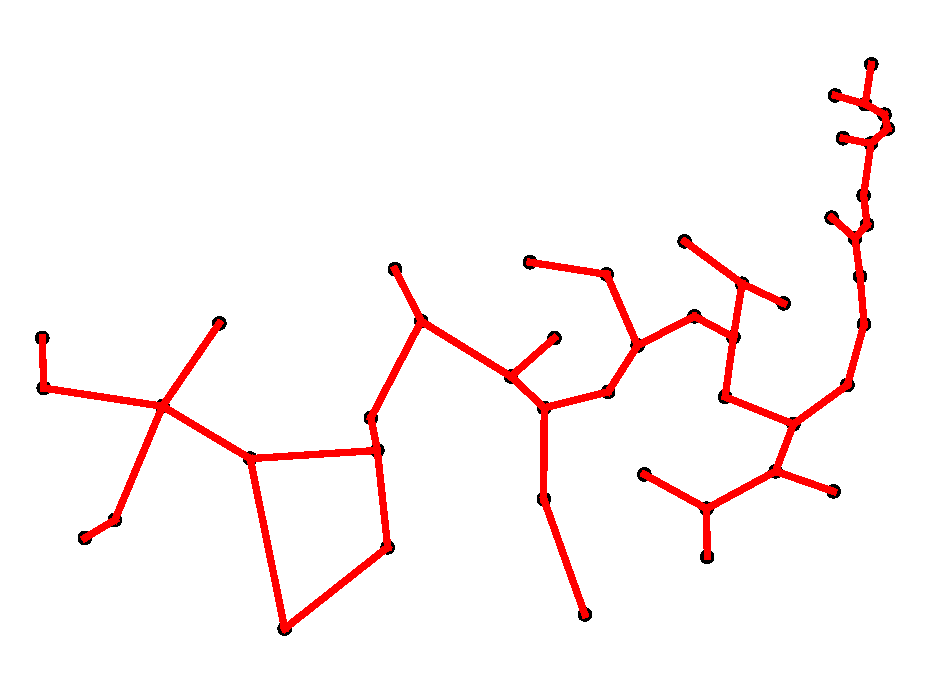
\includegraphics[width=.33\linewidth]{1MST Init.pdf}}
    \subfloat[优化$\mathcal{T_{\pi}}$ \label{subfig:优化1MST}]{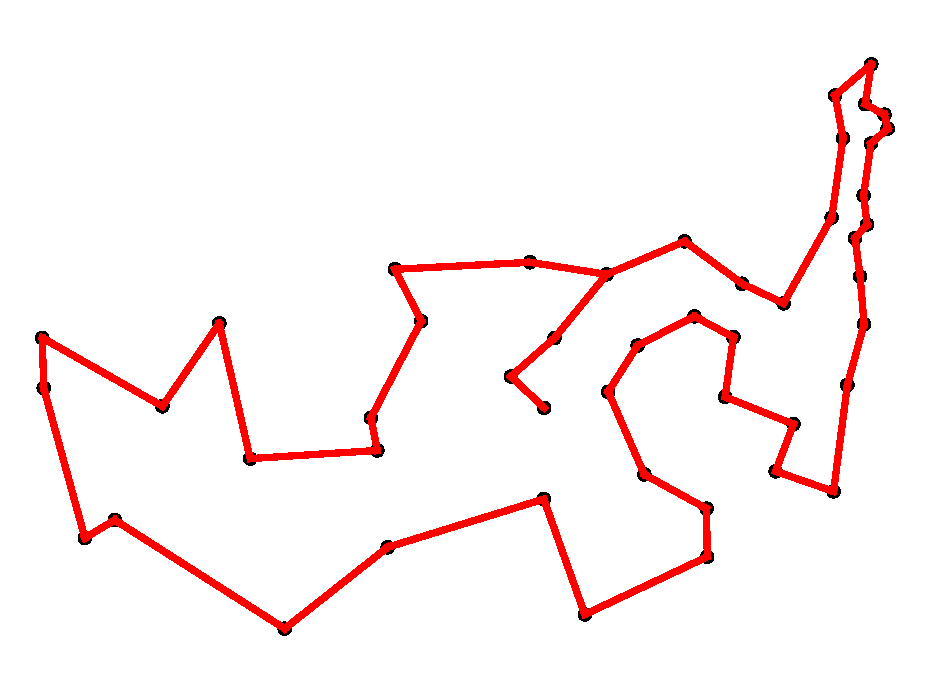
\includegraphics[width=.33\linewidth]{1MST Improved.pdf}}
    \subfloat[最优Tour \label{subfig:最优Tour}]{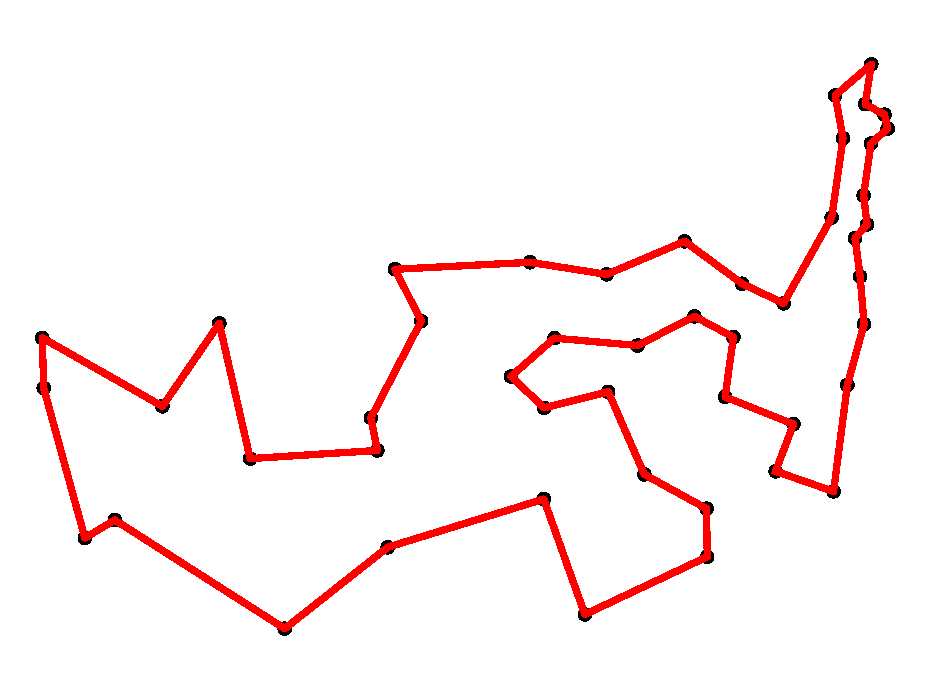
\includegraphics[width=.33\linewidth]{1MST Tour.pdf}}
    \caption[次梯度优化结果示意图]{次梯度优化结果示意图}
    \label{fig:次梯度优化结果示意图}
\end{figure}
\par
\autoref{fig:次梯度优化结果示意图}~中展示了1MST使用次梯度优化后的效果。\autoref{subfig:初始1MST}~是使用原始$W$获取的1MST,\autoref{subfig:优化1MST}~是原始$W$经过次梯度优化后获取的1MST,\autoref{subfig:最优Tour}~展示的是该问题的最优Tour。从图中可以看出,原始1MST经过次梯度优化后,节点的度数都趋向于2,并且包含了大量的最优Tour中的边。

\section{邻域结构生成算法}
\label{sec:NS_Method:邻域结构生成算法}
在这一节,首先将介绍基于最小生成树和欧拉回路的邻域结构(Neighborhood Structure based on Minimum spanning tree and Euler circuit,meNS)生成算法的主框架,然后会分节介绍算法中各个子部分。包括使用1MST来构造Tour以及使用循环扫描局部优化来对Tour进行初步的优化。

\subsection{meNS生成算法主框架}
\label{subsec:NS_Method:邻域结构生成算法:meNS主框架}
实现meNS生成算法的关键在于如何高效的生成一系列中等质量的初始Tour,因为这些初始Tour中必定包含大量的最优Tour中的边。算法利用这一系列中等质量的Tour,将其拆分并重新组装构造成一个完整的邻域结构。从算法~\ref{alg:次梯度优化}~可以知道,算法产生了大量的未被使用的1MST。而meNS生成算法的核心思想就是利用这些未被使用的1MST,用欧拉回路最为桥梁,将其转变为Tour。经过1MST转变来的Tour的质量会比随机生成的好很多,因此,这个步骤将节省大部分的优化时间。最后,只需要将这些Tour经过局部优化,就可以得到一个高质量的邻域结构。meNS生成算法主框架如下:
\par
\begin{algorithm}
    \setstretch{1.3}
    \caption{meNS生成算法主框架}
    \label{alg:meNS生成算法主框架}
    \BlankLine
    \KwIn{ \\
        \hspace{1.1em} $T \ $:$\{ \mathcal{T}_1, \cdots, \mathcal{T}_k \}$ \\
        \hspace{1em} $M$:最大候选边数 \\
        \hspace{1.1em} $L \ $:子路径长度 \\
        \hspace{1.1em} $S \ $:扫描次数
    }
    \KwOut{$meNS$}
    $meNS \leftarrow \varnothing$ \label{line:meNS初始化} \;
    \ForEach{$\mathcal{T} \in T$ \label{line:处理1MST}}{
        \tcp{通过$Transform$操作,将$\mathcal{T}$转变为$Tour$}
        $Tour \xleftarrow[]{Transform} \mathcal{T}$ \label{line:1MST转换} \;
        \tcp{通过循环扫描局部优化,对$Tour$进行优化得到$Tour'$}
        $Tour' \xleftarrow[]{Optimize} Tour, L, S$ \label{line:Tour局部优化} \;
        \tcp{将$Tour'$转换成边集并入到$meNS$中}
        $meNS \leftarrow meNS \bigcup Tour'$ \label{line:并入meNS} \;
    } \label{line:处理1MST结束}
    \tcp{修剪meNS,使得每个点的候选边不超过M条}
    $meNS \xleftarrow[]{Trim} meNS, M$ \label{line:修剪meNS} \;
    \textbf{return } $meNS$ \;
\end{algorithm}
\par
算法~\ref{alg:meNS生成算法主框架}~所示为meNS生成算法的主要步骤。第~\ref{line:meNS初始化}~是将邻域结构meNS初始化为空集。第~\ref{line:处理1MST}-\ref{line:处理1MST结束}~行循环处理1MST,将所有的1MST转变为Tour并将其优化。其中,第~\ref{line:1MST转换}~行是将1MST转变为Tour。第~\ref{line:Tour局部优化}~行是对转变得到的Tour进行循环扫描局部优化,得到优化后的$Tour'$。第~\ref{line:并入meNS}~行是将$Tour'$的边并入到邻域结构meNS中。最后,第~\ref{line:修剪meNS}~行是对meNS进行修剪,尽可能的使邻域结构稀疏化。

\subsection{1MST变换}
\label{subsec:NS_Method:邻域结构生成算法:1MST变换}
在算法~\ref{alg:meNS生成算法主框架}~中,第~\ref{line:1MST转换}~行使用$Transform$将1MST转换成Tour。在将1MST转换成Tour的过程中,需要先把1MST构造成欧拉回路(\autoref{def:Eulerian Cycle})。根据\autoref{thm:欧拉回路}~和\autoref{cor:欧拉回路}~可知,首先需要将1MST构造成每个点都为偶数度的连通图(欧拉图)。由\autoref{def:Tree}~,\autoref{def:Spanning 1-Tree}~和\autoref{def:Spanning 1-Tree}可知,1MST是具有偶数个(或0个)奇数度节点的连通图,因此,我们只需要将1MST所有的奇数度节点构造成偶数度节点,即可得到欧拉图。一个巧妙的构造方法是将这些奇数度节点根据节点之间的距离分成不同的组,每个组中有两个奇数度节点,然后将每组中的顶点用边链接起来,这样两个奇数度节点就变成了偶数度节点了。其构造过程如算法~\ref{alg:Transform}~第~\ref{line:构造成欧拉图}-\ref{line:构造成欧拉图结束}~行所示,其中第\ref{line:closest node}~行就是在$V_{odd}$中获取最近的两个奇度点$v_i, v_j$,第\ref{line:并边}~行将$v_i, v_j$链接成边$e_{i,j}$并入到$G_{euler}$中,最后第\ref{line:删点}~行从$V_{odd}$中删除$v_i, v_j$,最终获得的$G_{euler}$就是欧拉图了。
\par
\begin{algorithm}[htb]
    \setstretch{1.3}
    \caption{Transform}
    \label{alg:Transform}
    \BlankLine
    \KwIn{ \\
        \hspace{1em} $\mathcal{T} = (V, E) \ $:$1MST$
    }
    \KwOut{$Tour$}
    \tcp{初始化欧拉图$G_{euler}$和奇数度点集$V_{odd}$}
    $G_{euler} \xleftarrow[]{\{ e_{i,j} \ | \ e_{i,j} \in E \}} \mathcal{T} $ \label{line:init}\;
    $V_{odd} \xleftarrow[]{} \varnothing $ \;
    \ForEach{$v \in V$}{
        \lIf{$v$ is odd degree}{
            $V_{odd} \leftarrow V_{odd} \bigcup v$
        }
    } \label{line:init end}
    \tcp{将1MST构造成欧拉图}
    \While{$V_{odd} \not = \varnothing$ \label{line:构造成欧拉图}}{
        $v_i, v_j = argmin(\{ d(v_i, v_j) \ | \ v_i, v_j \in V_{odd}, i \not = j \}) $ \label{line:closest node} \;
        $G_{euler} \leftarrow G_{euler} \bigcup (e_{i, j} = (v_i, v_j)) $ \label{line:并边} \;
        $V_{odd} \leftarrow V_{odd}/\{v_i, v_j\}$ \label{line:删点} \;
    } \label{line:构造成欧拉图结束}
    \tcp{从欧拉图中通过\autoref{eq:从欧拉图中获取欧拉回路}~获取欧拉回路}
    $C_{euler} \xleftarrow[]{\text{式}\eqref{eq:从欧拉图中获取欧拉回路}} G_{euler}$ \label{line:从欧拉图中获取欧拉回路} \;
    \tcp{将欧拉回路通过\autoref{eq:将欧拉回路构造成Tour}~构造成Tour}
    $Tour \xleftarrow[]{\text{式}\eqref{eq:将欧拉回路构造成Tour}} C_{euler}$ \label{line:将欧拉回路构造成Tour} \;
    \textbf{return } $Tour$ \;
\end{algorithm}
\par
在算法~\ref{alg:Transform}~中,第~\ref{line:init}-\ref{line:init end}~行是初始化阶段,主要作用就是初始化欧拉图和奇数度点集,将1MST中的边并入到初始欧拉图中,并将奇数度点加入到奇数度点集中。第~\ref{line:构造成欧拉图}-\ref{line:构造成欧拉图结束}~行主要是将1MST构造成欧拉图的流程。第\ref{line:从欧拉图中获取欧拉回路}~行通过\autoref{eq:从欧拉图中获取欧拉回路}~从欧拉图中获取欧拉回路:
\vspace{-.5em}
\begin{align}
    \label{eq:从欧拉图中获取欧拉回路}
    C_{euler} = <v_i, v_j, v_k, \cdots, v_m, v_n, v_i>, \\
    \{e_{i,j}, e_{j,k}, \cdots, e_{m,n}, e_{n,i}\} = G_{euler}, \notag \\ 
    e_{i,j} = (v_i, v_j) \in G_{euler}, \ i \not = j. \notag 
\end{align}
\vspace{-.5em}
其中,欧拉回路$C_{euler}$中路径序列所组成的边就是欧拉图$G_{euler}$中的所有边,且这些边不重复,但是点可以重复使用。在第\ref{line:将欧拉回路构造成Tour}~行通过\autoref{eq:将欧拉回路构造成Tour}~将欧拉回路构造成Tour:
\vspace{-.5em}
\begin{align}
    \label{eq:将欧拉回路构造成Tour}
    Tour = <v_i, v_j, \cdots, v_n, v_i>, \\ 
    v_i, \cdots, v_n \in C_{euler}, \ i \not = n. \notag
\end{align}
其中,Tour是按照欧拉回路$C_{euler}$中路径序列的顺序,去除重复的点所构成的一个路径序列。可以知道Tour也包含了欧拉图中的所有点,除去首尾节点相同,其他节点都不相同。
\par
\autoref{fig:1MST构造Tour示意图}~所示是一个1MST转换为Tour的具体实例。其中\autoref{subfig:1MST}~展示的是1MST,它包含了四个奇数度节点$V_{odd} = \{v_3,v_4,v_5,v_6\}$,根据算法~\ref{alg:Transform}~第~\ref{line:构造成欧拉图}-\ref{line:构造成欧拉图结束}~行,可以将$V_{odd} = \{v_3,v_4,v_5,v_6\}$中的四个点分成$\{v_3,v_6\}$和$\{v_4,v_5\}$两组,然后将两组中的点分别链接起来得到两条边$e_{3,6} = (v_3,v_6)$和$e_{4,5} = (v_4,v_5)$,然后将$e_{3,6}$和$e_{4,5}$并入到$G_{euler}$中,最终获取到的$G_{euler}$为欧拉图,如\autoref{subfig:欧拉图}~所示,其中红色的边即为$e_{3,6}$和$e_{4,5}$。然后遍历欧拉图$G_{euler}$中的边,根据\autoref{eq:从欧拉图中获取欧拉回路}~可以得到一条欧拉回路$C_{euler} = <v_1, v_9, v_7, v_3, v_6, v_3, v_2, v_4, v_5, v_4, v_8, v_{10}, v_1>$,最后根据\autoref{eq:将欧拉回路构造成Tour}~,删除欧拉回路$C_{euler}$中重复的点,可以得到其中一条$Tour = <v_1, v_9, v_7, v_3, v_6, v_2, v_4, v_5, v_8, v_{10}, v_1>$,如\autoref{subfig:Tour}~所示。
\par
\begin{figure}[htb]
    \subfloat[最小生成1-tree \label{subfig:1MST}]{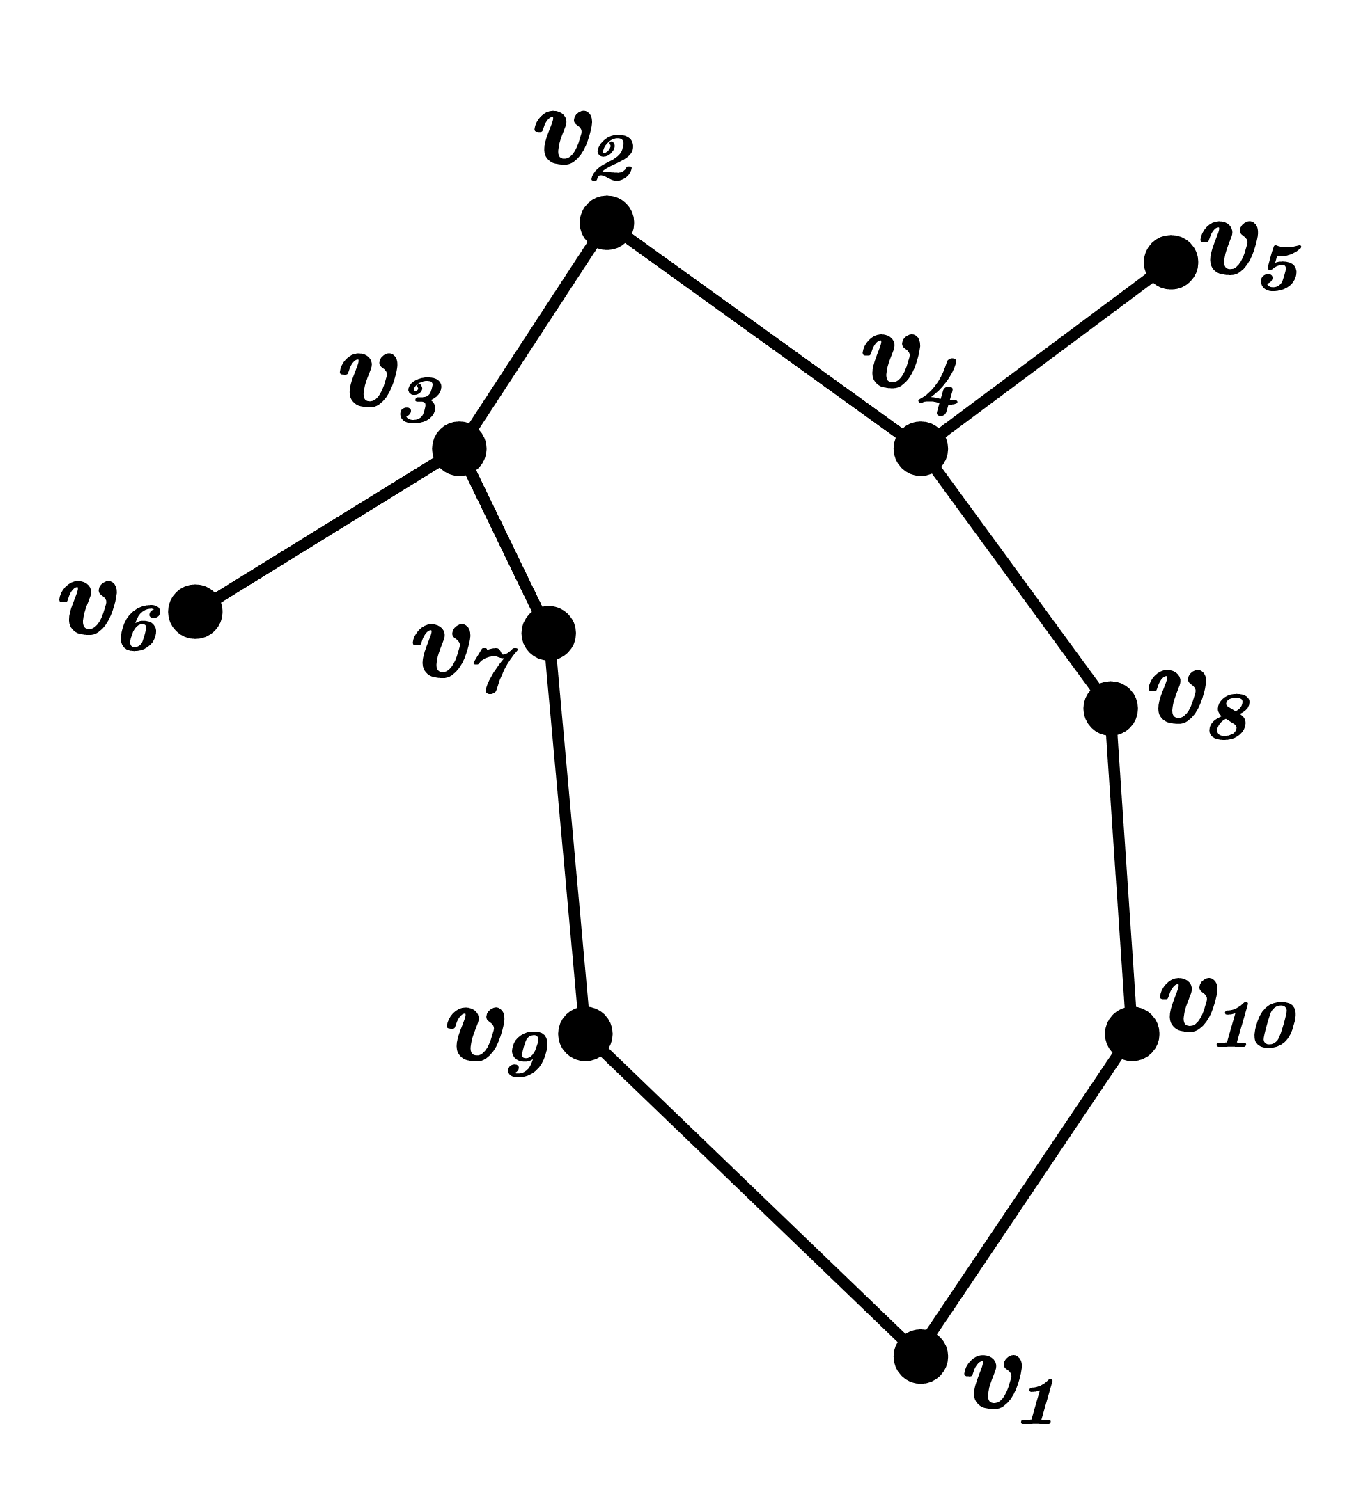
\includegraphics[width=.33\linewidth]{Transform-1MST.pdf}}
    \subfloat[欧拉图 \label{subfig:欧拉图}]{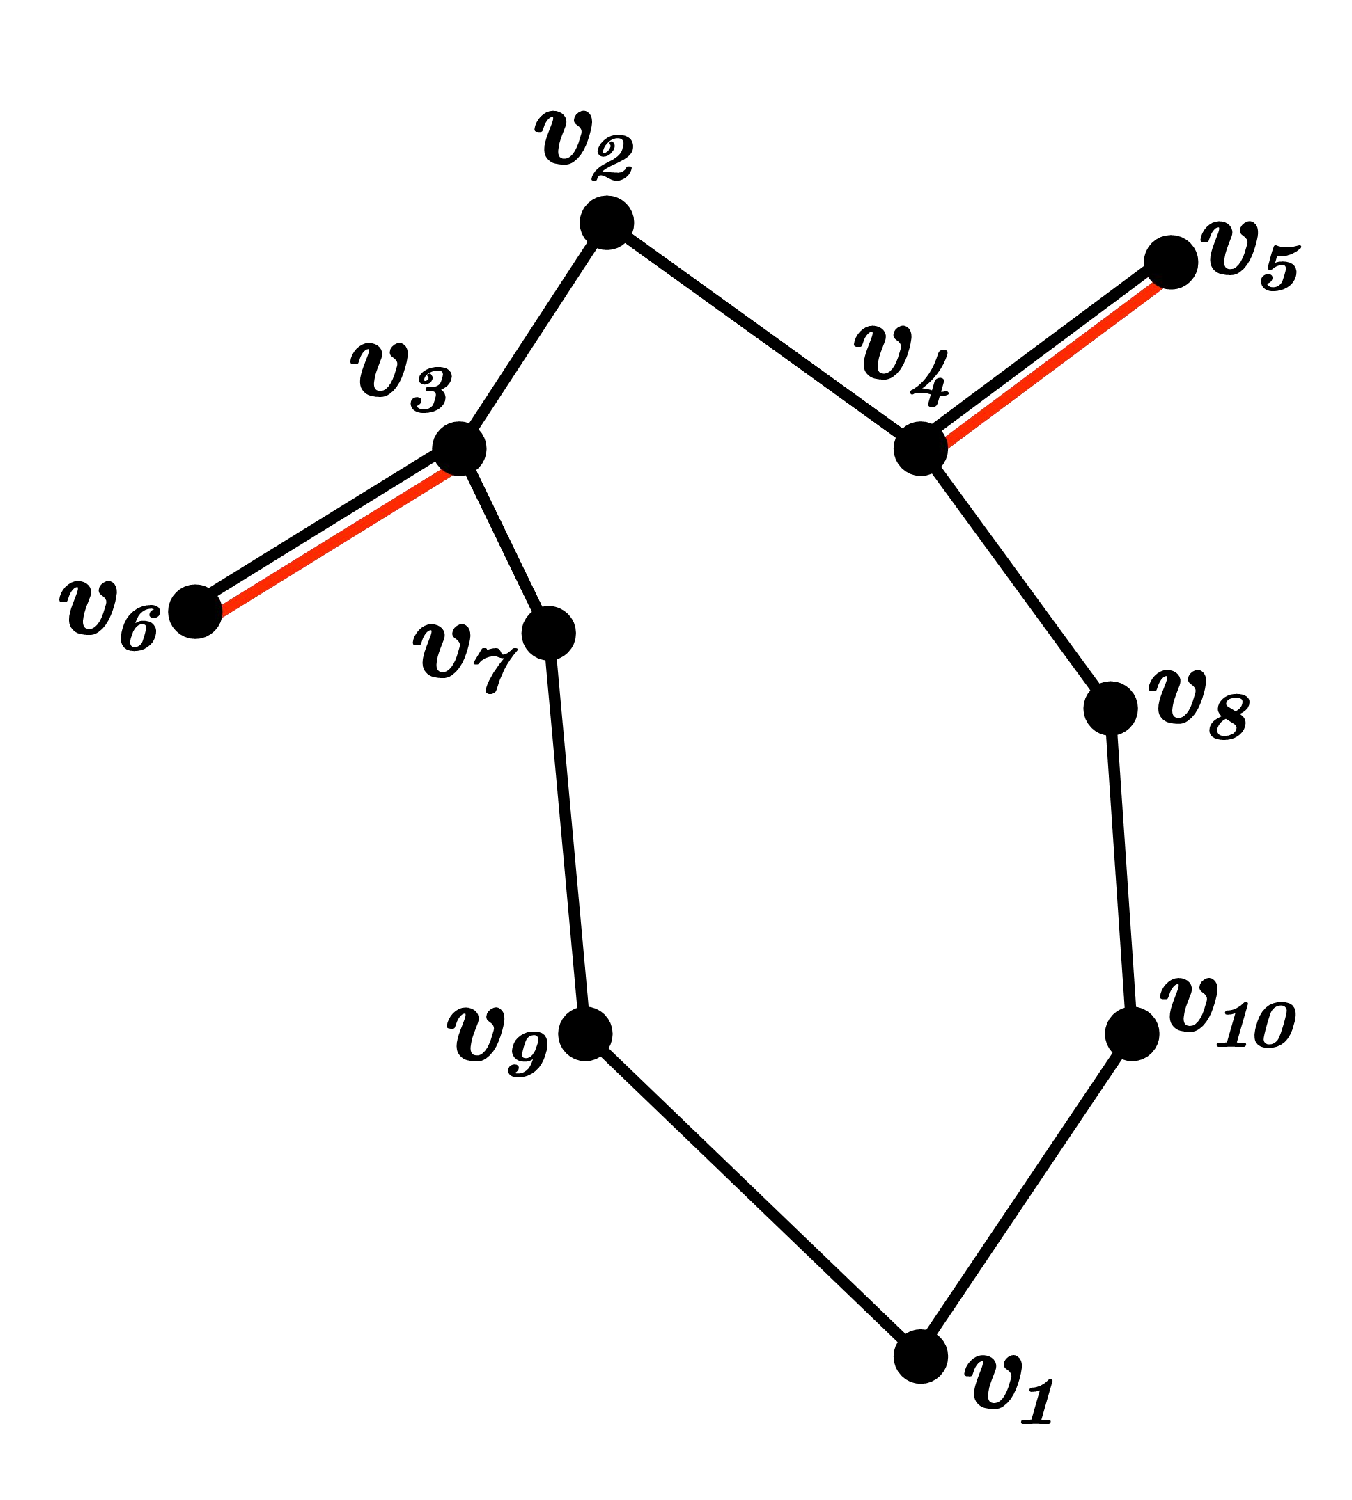
\includegraphics[width=.33\linewidth]{Transform-Euler Graph.pdf}}
    \subfloat[Tour \label{subfig:Tour}]{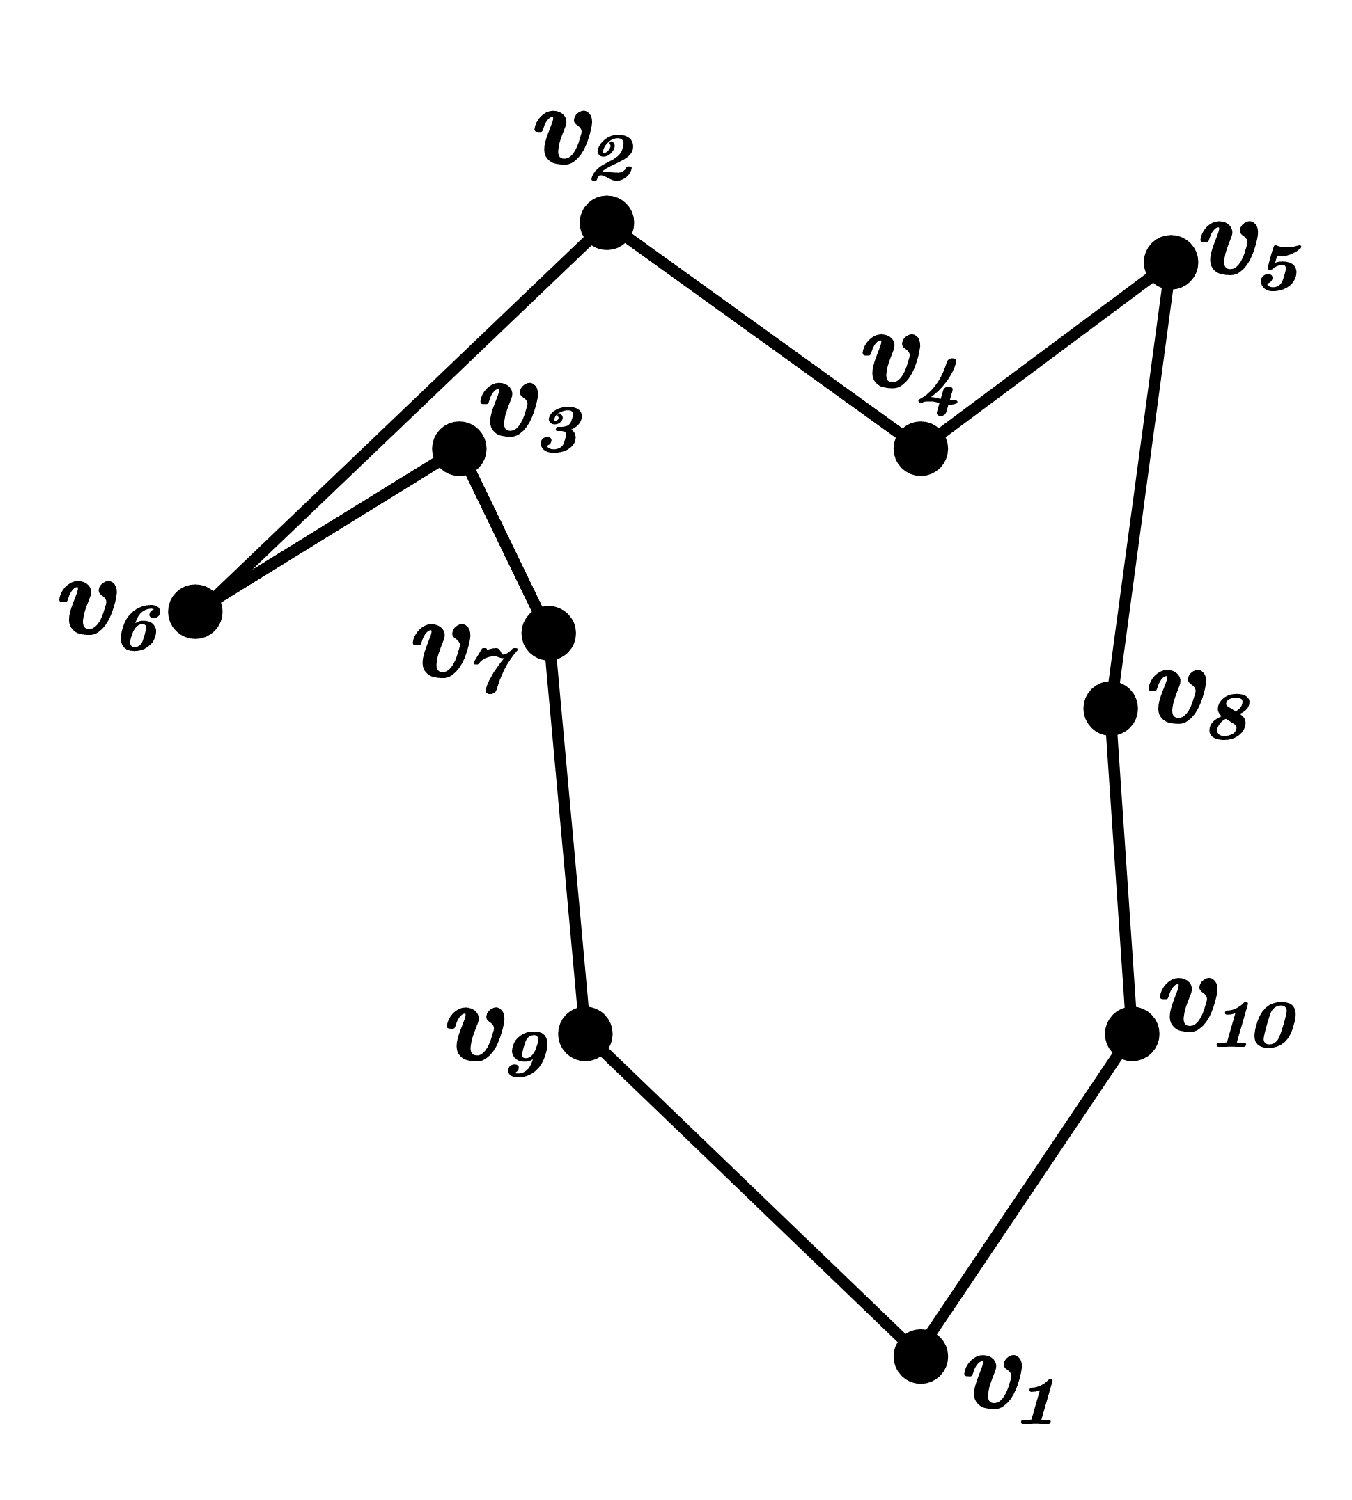
\includegraphics[width=.33\linewidth]{Transform-Tour.pdf}}
    \caption[1MST构造Tour示意图]{1MST构造Tour示意图}
    \label{fig:1MST构造Tour示意图}
\end{figure}

\subsection{循环扫描局部优化}
\label{subsec:NS_Method:邻域结构生成算法:循环扫描局部优化}
在章节~\ref{subsec:NS_Method:邻域结构生成算法:1MST变换}~中,算法~\ref{alg:Transform}~将1MST构造成了一系列的Tour,本节将介绍一种局部优化的方法,对这些Tour进行更进一步的优化,使得这些Tour尽可能的贴近最优Tour,从而包含更多的最优Tour中的边,以致最终获得的邻域结构的质量更好。其算法流程如下:在算法的输入参数中,$Tour$为待优化的巡回路径;$L$为子路径的长度,因为在算法中,局部优化是以$L$长度为单位进行的,这样就把整个$Tour$分成了$n/L$份,然后对每一个长为$L$的子路径进行局部优化;$S$为算法整体的扫描次数,因为每次扫描后,对整个$Tour$只做了局部的优化,然后对$Tour$通过循环右移的操作将之前的局部性重置,接着再次优化,最后通过多次这样的扫描,使得$Tour$整体都得到优化。
\begin{algorithm}[htb]
    \setstretch{1.3}
    \caption{循环扫描局部优化}
    \label{alg:循环扫描局部优化}
    \BlankLine
    \KwIn{ \\
        \hspace{1.1em} $Tour \ $:待优化Tour \\
        \hspace{1.1em} $L \ $:子路径长度 \\
        \hspace{1.1em} $S \ $:扫描次数
    }
    \KwOut{$Tour \ $:优化后Tour}
    \tcp{Comment}
    $n = |Tour|$ \label{line:节点数} \;
    \For{$i = 1 \ $ to $\ S$ \label{line:扫描}}{
        \lIf{$i \not = 1$}{
            $Tour \xleftarrow[]{\text{循环右移}} Tour, L, S$ \label{line:循环右移}
        }
        \For{$j =0 \ $ to $\ \lfloor n/L \rfloor - 1 $}{
            $Tour \xleftarrow[]{2-opt} Tour, L, jL$ \label{line:局部优化1} \;
        }
        \lIf{$n \% L \not = 0$}{
            $Tour \xleftarrow[]{2-opt} Tour, L, n-L$ \label{line:局部优化2} 
        }
    }\label{line:扫描结束}
    \textbf{return } $Tour$ \;
\end{algorithm}
\par
如算法~\ref{alg:循环扫描局部优化}~所示,第~\ref{line:节点数}~行中$|\cdot|$表示集合中元素的个数。第~\ref{line:扫描}-\ref{line:扫描结束}~行是$S$次扫描优化的过程。其中第~\ref{line:循环右移}~是对$Tour$进行整体循环右移$L/S$位,这样可以打破原有的局部性,使得$Tour$能够在全局上得到优化。第~\ref{line:局部优化1}~行和第~\ref{line:局部优化2}~是分别对前$\lfloor n/L \rfloor - 1$个子路径和最后一个子路径进行优化,其中,用到的局部优化算子为2-opt(如\autoref{subfig:2-opt}),因为2-opt的低复杂度能够使子路径快速被优化。循环扫描局部优化如\autoref{fig:循环扫描局部优化示意图}~所示,每次只优化长度为$L$的子路径,再进行了整体的局部优化后,将$Tour$整体向右循环移动$L/S$个位置,经过$S$遍循环扫描后,$Tour$就整体右移了$L$个位置,刚好是一个子路径的长度,这样使得原来优化的局部性通过循环右移的操作扩散到全局,从而使得$Tour$得到了全局性的优化。
\begin{figure}[!htb]
    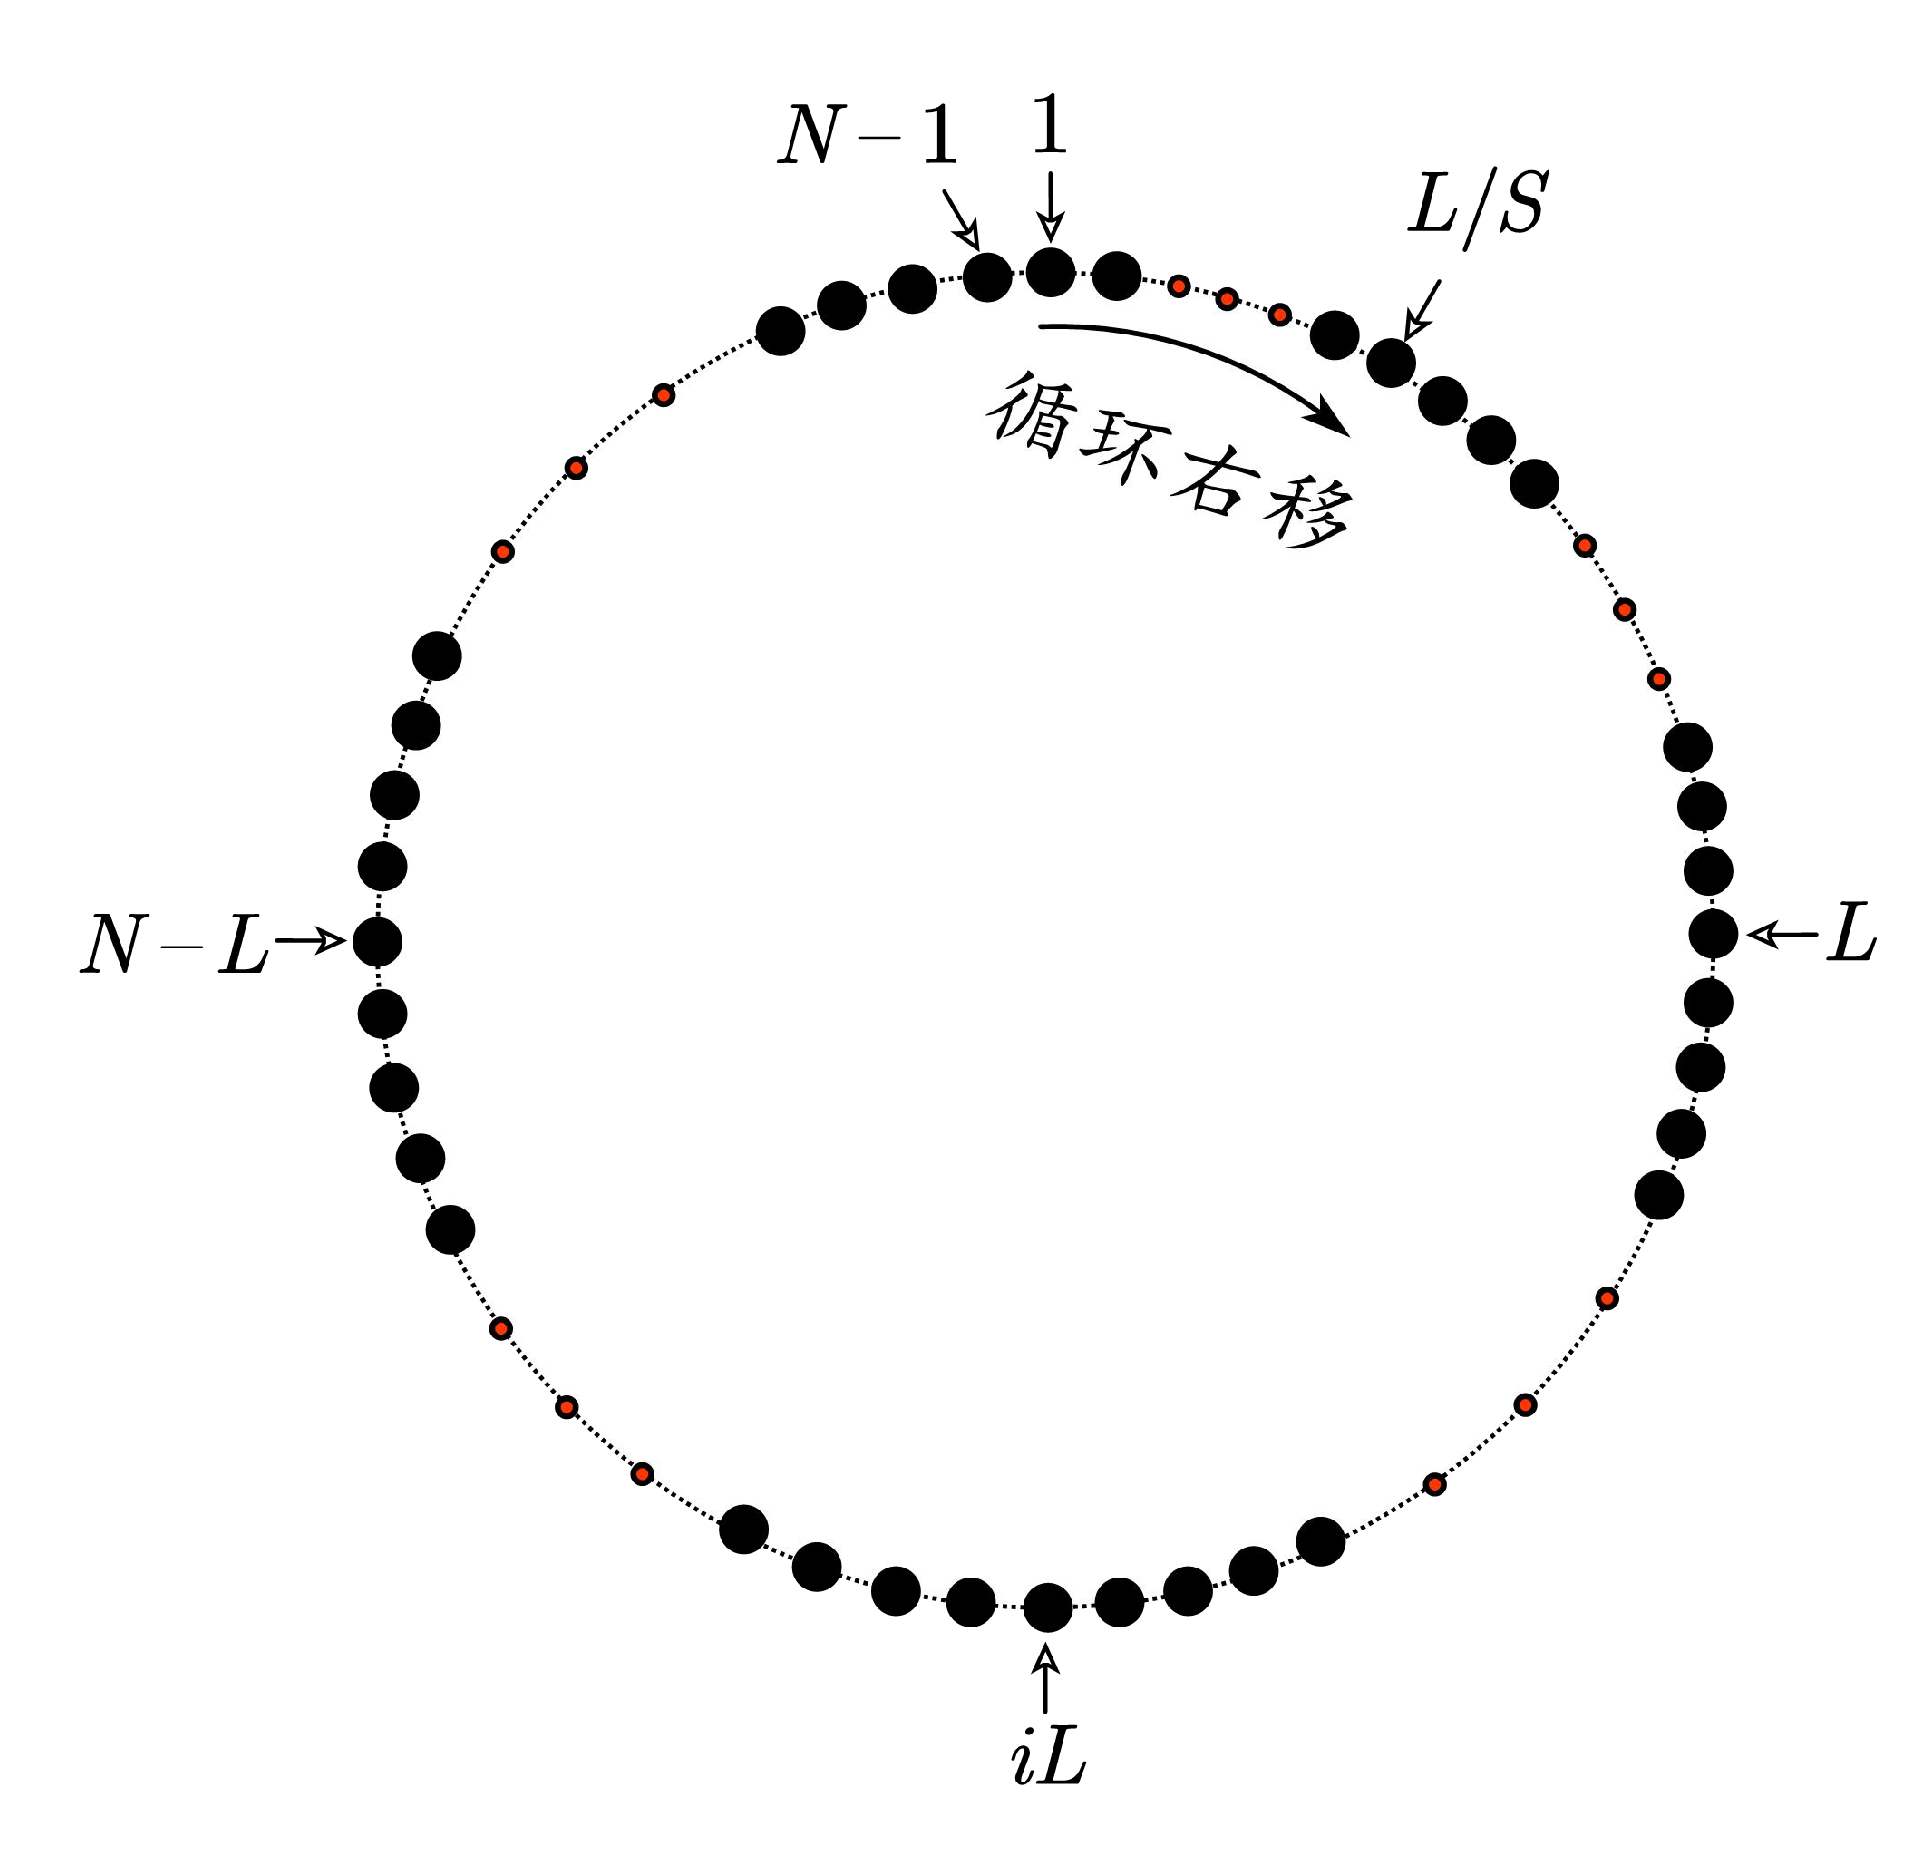
\includegraphics[width=.45\linewidth]{循环右移.pdf}
    \caption[循环扫描局部优化示意图]{循环扫描局部优化示意图}
    \label{fig:循环扫描局部优化示意图}
\end{figure}

\section{实验与讨论}
\label{sec:NS_Method:实验与讨论}

\subsection{实验设置及测试集}
\label{subsec:NS_Method:实验与讨论:测试集}
本节是对邻域结构生成方法进行实验,所有程序都是在Windows 10操作系统,2.4GHz的Intel i7 CPU和8G RAM的笔记本电脑上完成的。
\par
本实验使用的测试集都来自于DIMACS TSP竞赛\footnote{http://dimacs.rutgers.edu/archive/Challenges/TSP/}和TSPLIB\footnote{http://comopt.ifi.uni-heidelberg.de/software/TSPLIB95/}。包括了聚类型测试用例、均匀分布型测试用例、印刷电路板测试用例和真实地理位置测试用例,它们能够从各个方面体现算法生成的邻域结构的质量优劣,其具体信息如\autoref{tab:邻域结构测试集}~:
\begin{table}[htb]
    \caption[邻域结构测试集]{邻域结构测试集\label{tab:邻域结构测试集}}
    \begin{tabular}{llll}
        \toprule
        测试集类型 & 测试用例名称 & 节点数   & 权重类型 \\
        \midrule
        \multirow{5}[2]{*}{聚类型} & C1k   & 1000  & EUC\_2D \\
              & C3k   & 3162  & EUC\_2D \\
              & C10k  & 10000 & EUC\_2D \\
              & C31k  & 31623 & EUC\_2D \\
              & C100k & 100000 & EUC\_2D \\
        \midrule
        \multirow{5}[2]{*}{均匀分布型} & E1k   & 1000  & EUC\_2D \\
              & E3k   & 3162  & EUC\_2D \\
              & E10k  & 10000 & EUC\_2D \\
              & E31k  & 31623 & EUC\_2D \\
              & E100k & 100000 & EUC\_2D \\
        \midrule
        \multirow{2}[2]{*}{印刷电路板} & pla7397 & 7397  & CEIL\_2D \\
              & pla85900 & 85900 & CEIL\_2D \\
        \midrule
        真实地理位置 & brd14051 & 14051 & EUC\_2D \\
        \bottomrule
    \end{tabular}%
\end{table}
\par
在\autoref{tab:邻域结构测试集}~中,权重类型\cite{reinelt1995tsplib95}有两种,除了印刷电路板测试用例的权重类型是$CEIL\_2D$外,其他的测试用例的权重类型都为$EUC\_2D$,其计算公式如下:
\begin{itemize}
    \item $EUC\_2D$为二维欧几里得权重,设有两点及其坐标$v_i = (x_i, y_i)$和$v_j = (x_j, y_j)$,则边$e_{i,j}$的权重为:
    \vspace{-1.5em}
    \begin{align}
        \label{eq:EUC2D}
        w_{i,j} = \lfloor \sqrt{(x_i-x_j)^2 + (y_i-y_j)^2} + 0.5 \rfloor .
    \end{align}
    \vspace{-1.5em}
    \item $CEIL_2D\_2D$为二维向上取整的欧几里得距离,设有两点及其坐标$v_i = (x_i, y_i)$和$v_j = (x_j, y_j)$,则边$e_{i,j}$的权重为:
    \vspace{-1.5em}
    \begin{align}
        \label{eq:CEIL2D}
        w_{i,j} = \lceil \sqrt{(x_i-x_j)^2 + (y_i-y_j)^2} \rceil .
    \end{align}
\end{itemize}
\par
同时,为了测试算法的性能,本章主要用到了距离趋近度指标(章节~\ref{subsec:背景介绍:性能评价指标:距离趋近度指标})和最优边遗失率指标(章节~\ref{subsec:背景介绍:性能评价指标:最优边遗失率指标})来衡量算法生成的邻域结构的质量。

\subsection{meNS的质量及其生成算法的效率}
\label{subsec:NS_Method:实验与讨论:meNS质量及其生成算法的效率}
在本节中,将会验证meNS生成算法的执行效率及其生成meNS的质量。从章节~\ref{sec:NS_Method:邻域结构生成算法}~中可以知道,meNS生成算法是从大量的1MST中构造出一系列的Tour,这些Tour也可以被看作是问题的一个解。而meNS的最终质量也取决于这些被优化后的Tour的质量,因为meNS是由这些Tour的边构成的。从章节~\ref{subsec:NS_Method:邻域结构生成算法:meNS主框架}~中的算法~\ref{alg:meNS生成算法主框架}~可以知道,meNS生成算法可以分成两个子部分:获取初始Tour和优化Tour。将1MST转变为Tour的操作就属于第一个部分,也正是这个部分不仅能提高最终生成邻域结构的质量,还能节省算法的时间,下面将比较meNS生成算法与随机初始Tour(raNS)的生成算法的效率和质量。
\begin{table}[htbp]
    \centering
    \caption{meNS生成算法的效率和质量 \label{tab:meNS生成算法的效率和质量}}
    \begin{threeparttable}
        \begin{tabular}{ll|cc|cc|cc}
            \toprule
            \multirow{2}[4]{*}{测试用例} & \multirow{2}[4]{*}{节点数} & \multicolumn{2}{c}{Time (s)} & \multicolumn{2}{c}{Gap (\%)} & \multicolumn{2}{c}{Degree}                          \\
            \cmidrule{3-8}               &                            & meNS                         & raNS                       & meNS                       & raNS  & meNS & raNS  \\
            \midrule
            C1k                      & 1000                       & 0.38                         & 0.46                         & 11.62                      & 20.70  & 6.9  & 6.5    \\
            C3k                        & 3162                       & 1.90                         & 2.05                         & 9.66                       & 17.37  & 6.6  & 6.9    \\
            C10k                       & 10000                      & 6.43                         & 7.95                         & 13.50                      & 37.05  & 6.6  & 7.0    \\
            C31k                       & 31623                      & 12.28                        & 15.85                        & 11.47                      & 41.77  & 6.3  & 7.0    \\
            C100k                      & 100000                     & 51.26                        & 53.00                        & 12.38                      & 43.38  & 7.6  & 7.1    \\
            \midrule
            E1k                       & 1000                       & 0.44                         & 0.40                         & 8.16                       & 14.28  & 6.8  & 7.1    \\
            E3k                        & 3162                       & 2.10                         & 2.26                         & 9.30                       & 17.37  & 6.7  & 7.4    \\
            E10k                       & 10000                      & 6.40                         & 7.50                         & 10.25                      & 20.12  & 7.0  & 7.6    \\
            E31k                       & 31623                      & 10.50                        & 15.01                        & 10.02                      & 21.93  & 6.6  & 7.8    \\
            E100k.0                      & 100000                     & 33.64                        & 51.81                        & 9.99                       & 22.90  & 6.5  & 7.8    \\
            \midrule
            pla7397                      & 7397                       & 1.80                         & 3.88                         & 9.82                       & 27.54  & 7.1  & 7.5    \\
            pla85900                     & 85900                      & 20.20                        & 37.94                        & 9.38                       & 27.00  & 7.0  & 7.9    \\
            \midrule
            brd14051                     & 14051                      & 6.42                         & 9.61                         & 8.27                       & 18.07  & 6.6  & 7.6    \\
            \bottomrule
        \end{tabular}
        \begin{tablenotes}
            \item meNS为meNS生成算法.
            \item raNS为随机初始Tour的生成算法.
        \end{tablenotes}
    \end{threeparttable}
\end{table}
\par
\autoref{tab:meNS生成算法的效率和质量}~展示的是meNS生成算法(简称meNS)与随机初始Tour的生成算法(简称raNS)的效率和质量。在\autoref{tab:meNS生成算法的效率和质量}~中比较了meNS与raNS的三项指标,分别是算法生成邻域结构的时间、算法最终优化后的Tour的平均Gap(距离趋近度)指标和算法生成的邻域结构的平均稀疏度(节点的度)。
\par
从\autoref{tab:meNS生成算法的效率和质量}~中可以看出,meNS在三项指标上都要优于raNS。在算法生成邻域结构的时间上,如\autoref{fig:meNS与raNS时间对比示意图}~所示,虽然meNS和raNS随着节点数的增加,其时间增长速度都远低于二次方时间复杂度的增长速度,但是meNS在多种类型的测试用例上所用的时间都比raNS要少,这是因为,meNS在算法的第一阶段用1MST生成了大量的优质初始Tour,这个操作不仅能够使得算法节省生成Tour的时间,还能够使得算法在第二阶段优化这些Tour的时候更快的收敛到理想值。而raNS是随机产生的初始Tour,这个操作虽然用时可能更少,生成的初始Tour的质量不一定高,这使得算法在第二阶段需要花费大量的时间来进一步优化这些质量并不好的Tour,这导致算法整体的时间过长。在算法最终优化的Tour的平均Gap指标上,meNS生成的Tour的平均Gap指标只有raNS的一半左右,说明meNS生成的Tour更接近最优Tour,这意味着用这些Tour来构造邻域结构会包含更多的最优Tour中的边。在算法生成的邻域结构的平均稀疏度上,meNS生成的邻域结构也比raNS生成的邻域结构更稀疏,并且这是算法生成邻域结构后未被修剪的数据,这说明meNS生成的邻域结构更加精简,算法在使用时能够更快的收敛。
\begin{figure}[htb]
    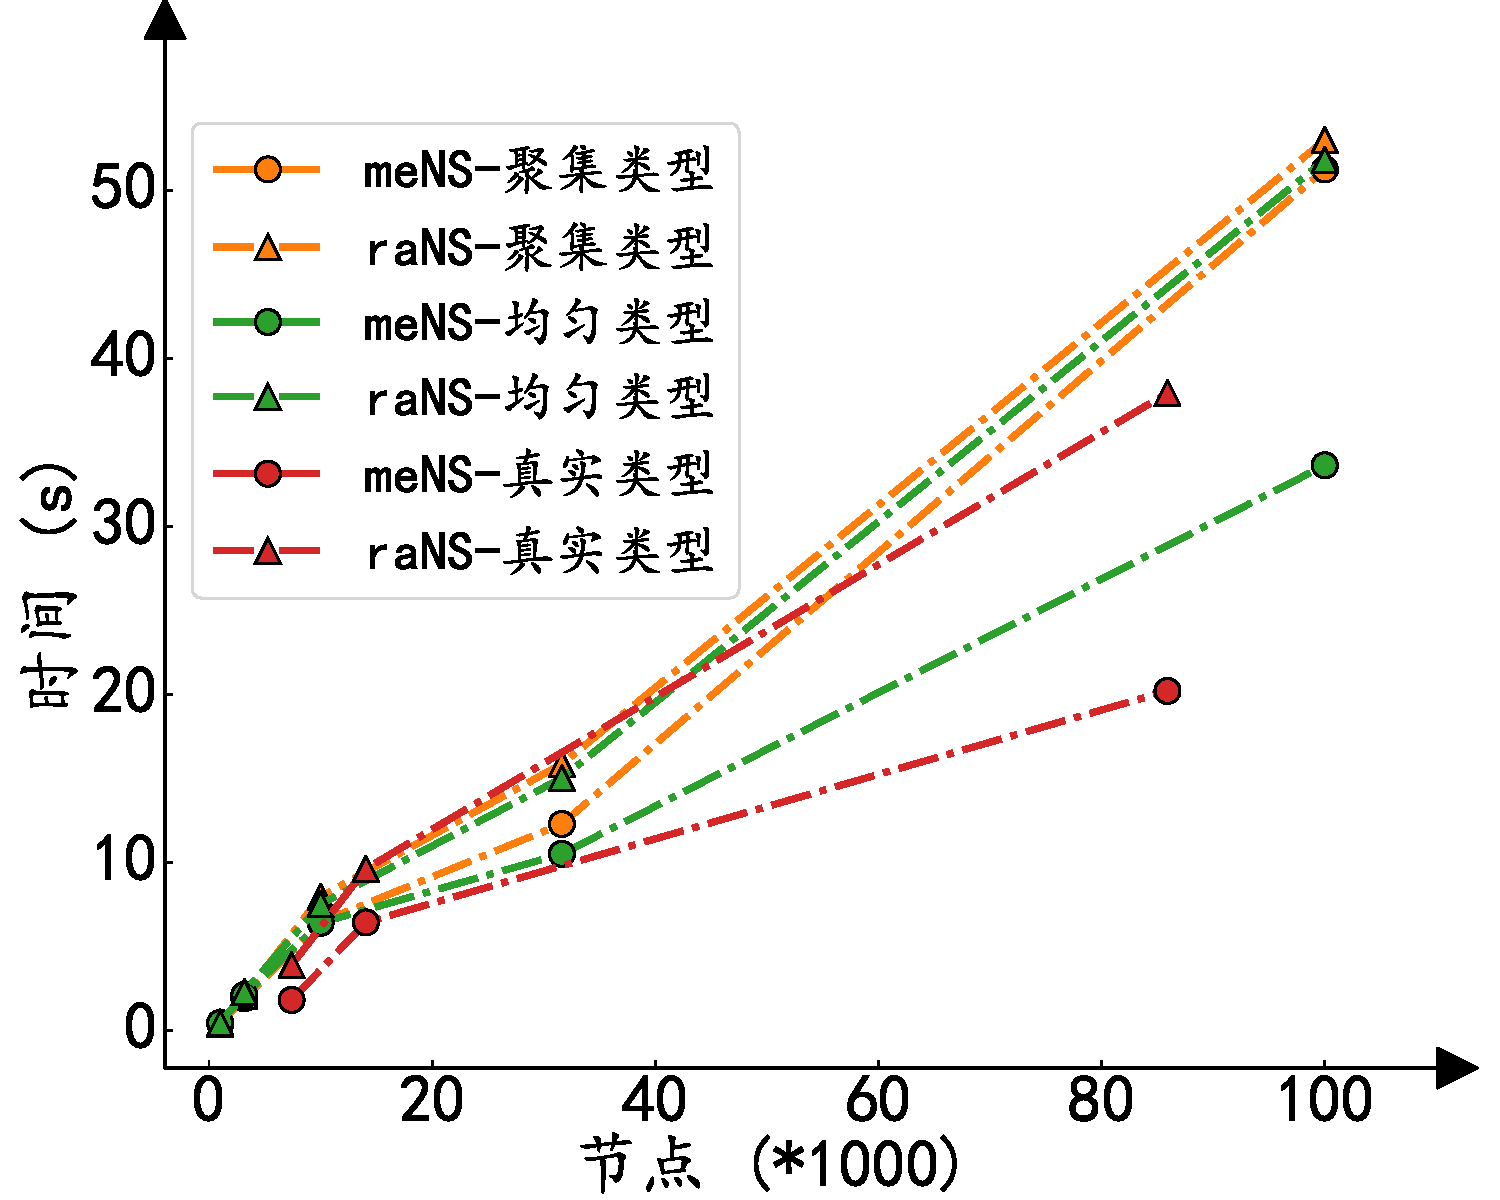
\includegraphics[width=.75\linewidth]{meNS时间对比.pdf}
    \caption[meNS与raNS时间对比示意图]{meNS与raNS时间对比示意图}
    \label{fig:meNS与raNS时间对比示意图}
\end{figure}

\subsection{meNS与其他邻域结构生成算法的比较}
\label{subsec:NS_Method:实验与讨论:meNS与其他邻域结构生成算法的比较}
在章节~\ref{subsec:NS_Method:实验与讨论:meNS质量及其生成算法的效率}~中,展示了meNS生成算法生成的未修剪的邻域结构的质量。在本节中,将会对比由meNS生成算法生成的修剪过的邻域结构与K最邻近(K-NN)、$\alpha$-nearest和三角剖分(Delaunay)算法生成的邻域结构的质量。由章节~\ref{subsec:NS_Method:邻域结构生成算法:meNS主框架}~中算法~\ref{alg:meNS生成算法主框架}~可知,邻域结构在经过进一步的优化后,还需要进行修剪。因为邻域结构的稀疏度关乎到算法的运行速度,邻域结构越稀疏,算法的收敛的就越快。但是,邻域结构又不能太稀疏,因为这可能使得邻域结构中包含最优Tour的边变少,所以,在算法中,使邻域结构中的每个点只保留$M$条边的方式来进行邻域结构的修剪,在本文中,所有的邻域结构的最大保留边都设为$M=5$。
\setlength{\tabcolsep}{13pt}
\begin{longtable}[c]{llllll}
    \caption{meNS与K-NN、$\alpha$-nearest和Delaunay邻域结构生成算法的邻域结构质量对比}\label{tab:各算法表现}\\
    \toprule
	测试用例  & 指标  & meNS  & K-NN  & $\alpha$-nearest & Delaunay \\ 
    \midrule
	\endfirsthead
	\multicolumn{6}{c}{\nuaafontcaption 续表~\thetable\hskip1em meNS与K-NN、$\alpha$-nearest和三角剖分邻域结构生成算法的邻域结构质量对比}\\
	\toprule
	测试用例  & 指标  & meNS  & K-NN  & $\alpha$-nearest & Delaunay \\ 
    \midrule
	\endhead
	\hline
	\multicolumn{6}{r}{续下页}
	\endfoot
	\endlastfoot
    \multirow{4}[2]{*}{C1k}    & Candidate Time (s) & 0.38    & 0.01   & 0.04    & 0.01   \\
                & NS Degree       & 4.6    & 5    & 5       & 5      \\
                & Missing (\%)              & 0.2000  & 3.0000  & 0.4000  & 0.5000  \\
                & LKH Gap (\%)           & 0.5438 & 0.5508 & 0.5438  & 0.5438 \\
    \midrule
    \multirow{4}[2]{*}{C3k}    & Candidate Time (s) & 1.9   & 0.15   & 0.77   & 0.02   \\
                & NS Degree       & 4.6    & 5    & 5       & 5      \\
                & Missing (\%)               & 0.1898  & 2.7514  & 0.4111  & 0.2530  \\
                & LKH Gap (\%)           & 0.6179 & 0.6415 & 0.6179  & 0.6179 \\
    \midrule
    \multirow{4}[2]{*}{C10k}   & Candidate Time (s) & 6.43  & 2.15  & 10.19   & 0.01  \\
                & NS Degree       & 4.6    & 5    & 5       & 5      \\
                & Missing (\%)               & 0.4400  & 2.3800 & 0.3200  & 0.2900  \\
                & LKH Gap (\%)           & 0.6688 & 0.7171 & 0.7966  & 0.7412 \\
    \midrule
    \multirow{4}[2]{*}{C31k}   & Candidate Time (s) & 12.28 & 19.72  & 141.82  & 0.15  \\
                & NS Degree       & 4.6    & 5    & 5       & 5      \\
                & Missing (\%)               & 0.2245  & 2.5140  & 0.3731  & 0.3384  \\
                & LKH Gap (\%)           & 0.5183 & 0.7077 & 1.7965  & 0.8065 \\
    \midrule
    \multirow{4}[2]{*}{C100k}  & Candidate Time (s) & 51.26 & 468.86 & 1612.35 & 0.55 \\
                & NS Degree       & 4.7    & 5    & 5       & 5      \\
                & Missing (\%)               & 0.13  & 2.403 & 0.363 & 0.353 \\
                & LKH Gap (\%)           & 0.1919 & 7.713 & 1.2847  & 1.5998 \\
    \midrule
    \multirow{4}[2]{*}{E1k}    & Candidate Time (s) & 0.44   & 0.02   & 0.04    & 0.01   \\
                & NS Degree       & 4.5    & 5    & 5       & 4      \\
                & Missing (\%)               & 0.2000  & 1.3000 & 0.3000  & 2.8000  \\
                & LKH Gap (\%)           & 0.7677 & 0.7967 & 0.7677  & 1.012  \\
    \midrule
    \multirow{4}[2]{*}{E3k}    & Candidate Time (s) & 2.1   & 0.16   & 0.78   & 0.03  \\
                & NS Degree       & 4.6    & 5    & 3.1     & 3.8    \\
                & Missing (\%)               & 0.2846  & 1.9608 & 2.0873  & 1.3599  \\
                & LKH Gap (\%)           & 0.7138 & 0.7826 & 1.057   & 0.8482 \\
    \midrule
    \multirow{4}[2]{*}{E10k}   & Candidate Time (s) & 6.4  & 2.07  & 10.14   & 0.2  \\
                & NS Degree       & 4.6    & 5    & 4.2     & 4.9    \\
                & Missing (\%)               & 0.1600  & 1.7100 & 0.4500  & 0.1500  \\
                & LKH Gap (\%)           & 0.7103 & 0.7758 & 0.7481  & 0.7104 \\
    \midrule
    \multirow{4}[2]{*}{E31k}   & Candidate Time (s) & 10.5 & 19.72  & 127.48  & 0.14  \\
                & NS Degree       & 4.6    & 5    & 5       & 5      \\
                & Missing (\%)              & 0.1708  & 1.7424 & 0.2340  & 0.2150  \\
                & LKH Gap (\%)           & 0.3615 & 0.7077 & 0.6505  & 0.6549 \\
    \midrule
    \multirow{4}[2]{*}{E100k}  & Candidate Time (s) & 33.64 & 434.29 & 1098.61 & 0.63 \\
                & NS Degree       & 4.6    & 5    & 5       & 5      \\
                & Missing (\%)               & 0.1920  & 1.7300 & 0.2770  & 0.2230  \\
                & LKH Gap (\%)           & 0.4078 & 0.7116 & 0.6687  & 0.6658 \\
    \midrule
    \multirow{4}[2]{*}{pla7397}  & Candidate Time (s) & 1.8   & 0.94  & 3.12   & 0.12  \\
                & NS Degree       & 4.4    & 5    & 4.9     & 4.9    \\
                & Missing (\%)               & 0.1352  & 0.8652 & 0.2433  & 0.2433  \\
                & LKH Gap (\%)           & 0.586  & 0.7725 & 0.5842  & 0.5806 \\
    \midrule
    \multirow{4}[2]{*}{pla85900} & Candidate Time (s) & 20.2 & 337.45 & 528.27 & 0.86 \\
                & NS Degree       & 4.5    & 5      & 4.8     & 4.8    \\
                & Missing (\%)               & 0.1630  & 0.2398 & 0.1281  & 0.1292  \\
                & LKH Gap (\%)           & 0.4701 & 1.5986 & 0.4774  & 0.4665 \\
    \midrule
    \multirow{4}[2]{*}{brd14051} & Candidate Time (s) & 6.42  & 166.33  & 17.51  & 0.51   \\
                & NS Degree       & 4.7    & 5      & 5       & 5      \\
                & Missing (\%)               & 0.0641  & 0.8042 & 0.1139  & 0.1139  \\
                & LKH Gap (\%)           & 0.4877 & 0.4949 & 0.4889  & 0.4883 \\
    \bottomrule
\end{longtable}
\par
\autoref{tab:各算法表现}~展示的是meNS与K-NN、$\alpha$-nearest和Delaunay算法生成的邻域结构的对比数据,并且在\autoref{tab:各算法表现}~中比较了各个算法生成的邻域结构在LKH算法\cite{helsgaun2000effective}(目前解决大型TSP问题最优秀的算法之一)中的表现,同时统计了各算法邻域结构生成时间(Candidate Time)、邻域结构的稀疏度(NS Degree)、最优边遗失率(Missing)和LKH最终解的距离趋近度(LKH Gap)四项指标数据。
\par
从\autoref{tab:各算法表现}~可以看出,在Candidate Time指标数据上,使用Delaunay生成的邻域结构耗费的时间比其他算法生成邻域结构花费的时间都要少,因为Delaunay算法采用分治的思想对整个图进行三角剖分,能够在$O(nlogn)$的时间复杂度内完成邻域结构的构建,但是Delaunay只能在二维坐标测试问题上有效生成邻域结构,当测试问题的坐标维度高于二维时,Delaunay算法就难以保持其高效性且算法会变得及其复杂。而K-NN和$\alpha$-nearest算法都是$O(n^2)$的时间复杂度,所以在构造邻域结构花费的时间最多,并且K-NN生成的邻域结构不需要修剪操作,所以K-NN生成邻域结构耗时比$\alpha$-nearest生成邻域结构耗时少。meNS生成算法构造邻域结构花费的时间介于Delaunay和K-NN、$\alpha$-nearest算法构造邻域结构花费的时间之间,从侧面也可以证明meNS生成算法的时间复杂度是低于二次方时间复杂度的。\autoref{fig:meNS和其他算法生成邻域结构时间对比示意图}~展示的是meNS生成算法和其他算法在不同类型测试用例构造邻域结构的时间示意图,从图中也能够得看出,meNS生成算法的高效性。
\begin{figure}[htb]
    \subfloat[聚类型 \label{subfig:聚类型}]{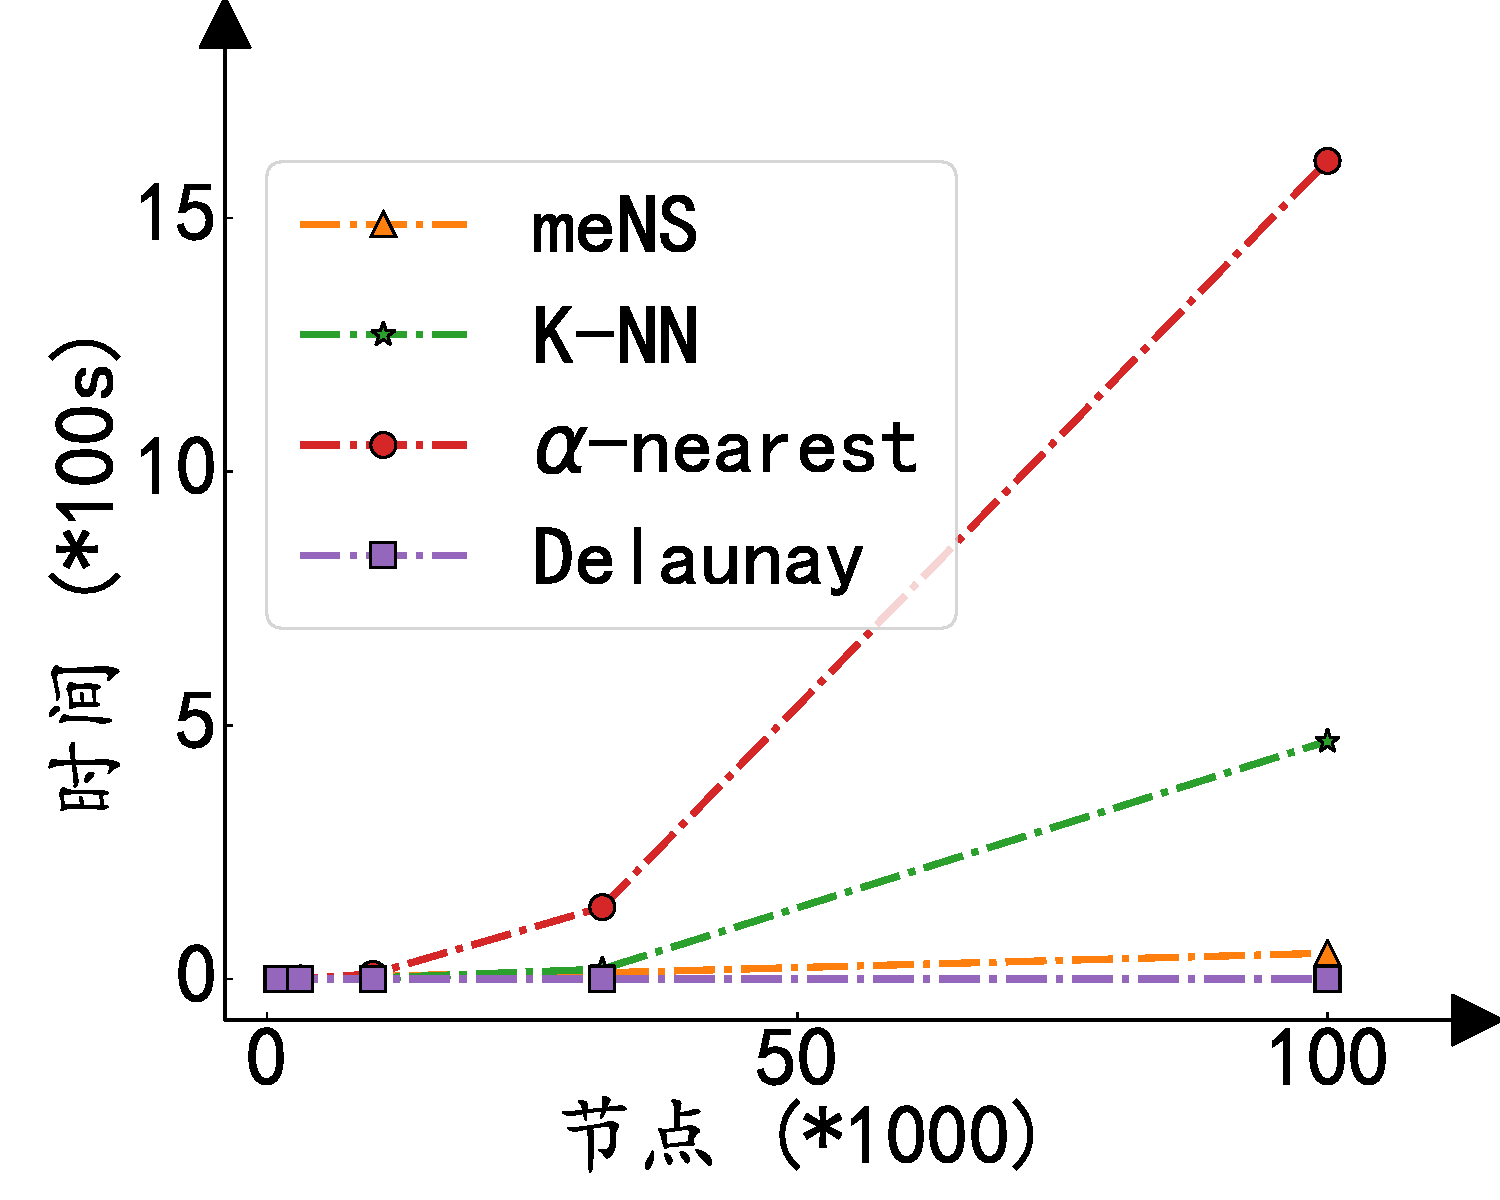
\includegraphics[width=.33\linewidth]{聚类型.can.pdf}}
    \subfloat[均匀分布型 \label{subfig:均匀分布型}]{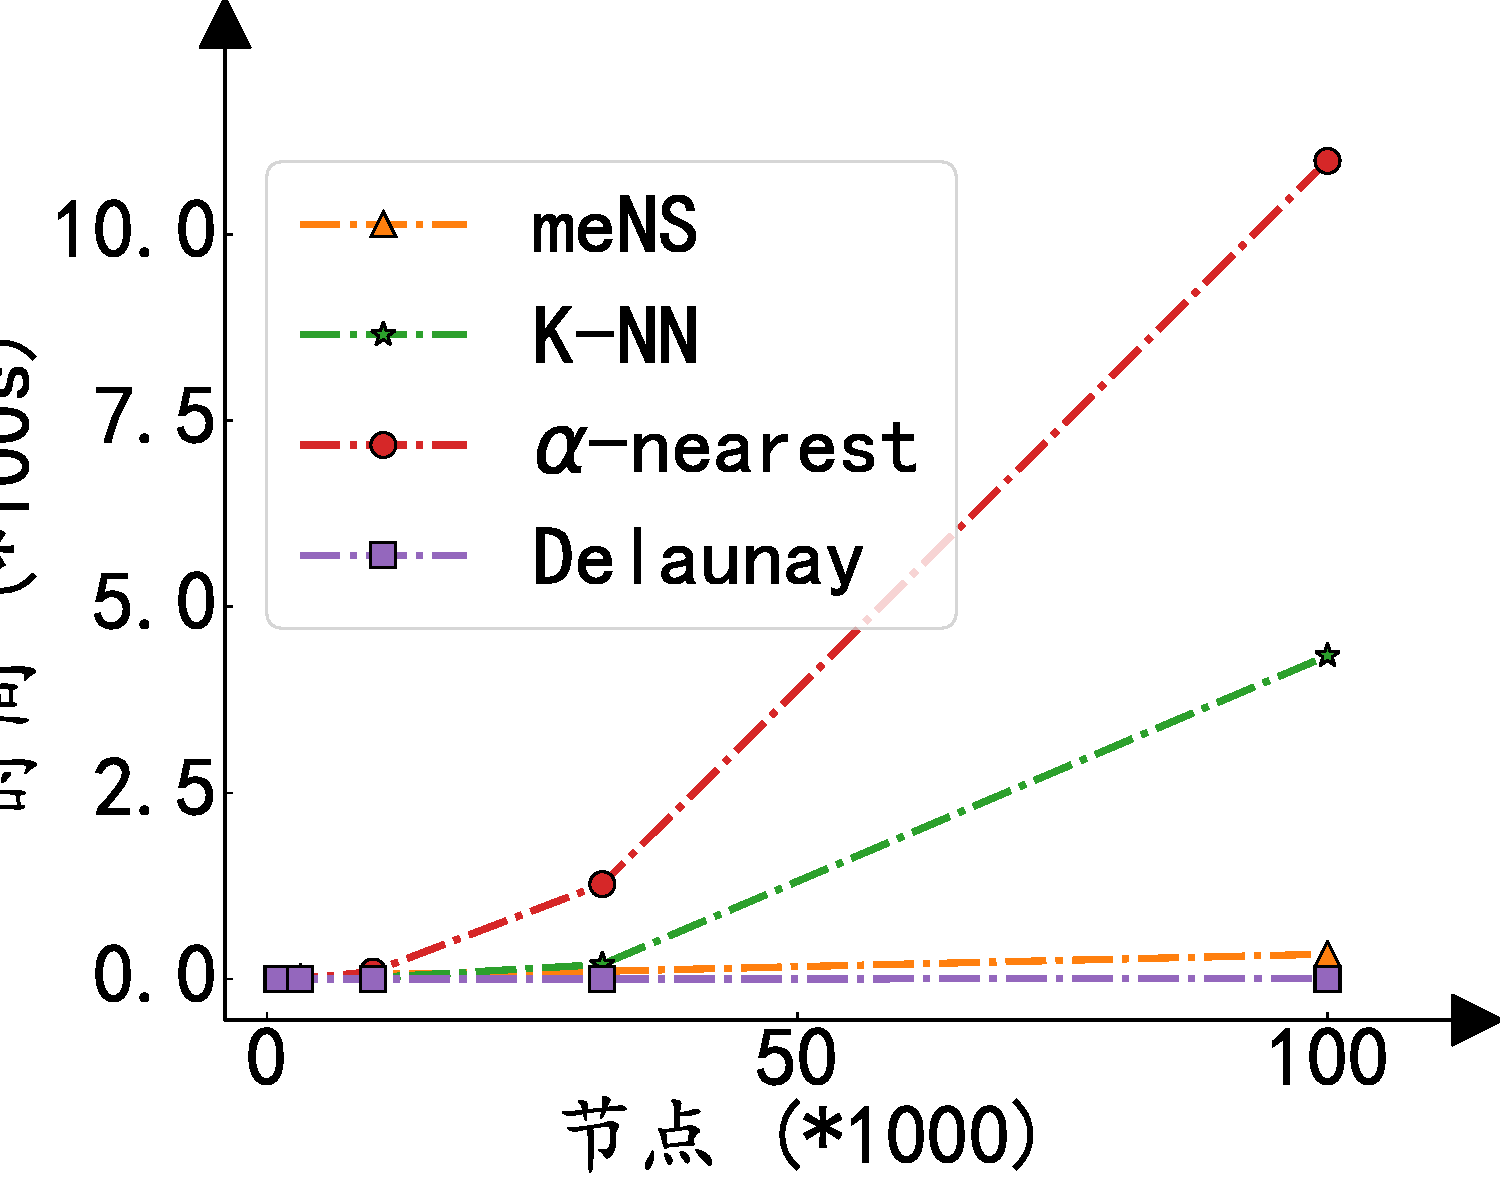
\includegraphics[width=.33\linewidth]{均匀分布型.can.pdf}}
    \subfloat[真实数据 \label{subfig:真实数据}]{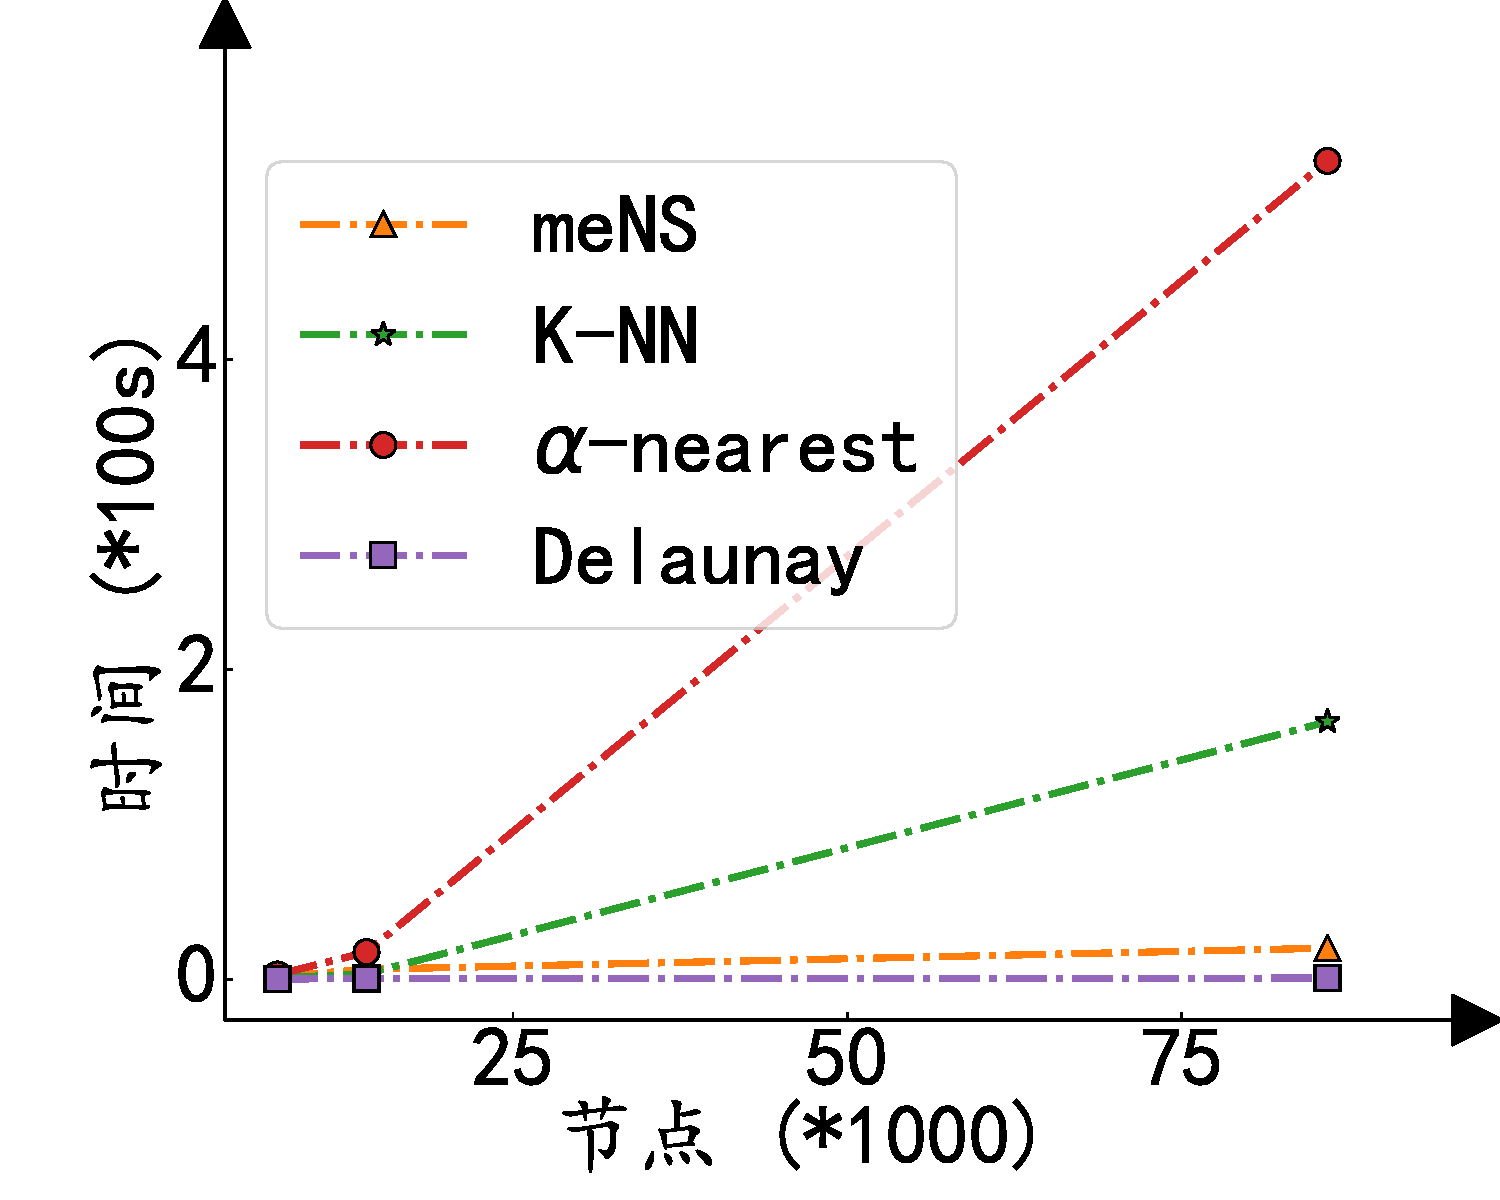
\includegraphics[width=.33\linewidth]{真实数据.can.pdf}}
    \caption[meNS和其他算法生成邻域结构时间对比示意图]{meNS和其他算法生成邻域结构时间对比示意图}
    \label{fig:meNS和其他算法生成邻域结构时间对比示意图}
\end{figure}
\par
在将各算法生成的邻域结构正式应用到LKH算法中之前,还需要对邻域结构进行修剪,以保证邻域结构的稀疏度。在本文中,邻域结构在修剪后,每个点最多只保留$M=5$条边作为其邻域。因此,从\autoref{tab:各算法表现}~中可以知道,在NS Degree指标数据上,所有的数值都不超过5,这就是对邻域结构修剪的结果。但是,在各数值上仍然能够得出,meNS生成算法的邻域结构修剪后要比其他生成算法修剪后的邻域结构更加稀疏,这使得该邻域结构用在求解算法中会收敛的更快,\autoref{fig:各算法在聚类型用例C3K生成的邻域结构}~、\autoref{fig:各算法在聚类型用例C3K生成的邻域结构}~,\autoref{fig:各算法在印刷电路板测试用例pla7397生成的邻域结构}~和\autoref{fig:各算法在真实地理位置测试用例brd14051生成的邻域结构}~中分别展示了各算法对于不同类型的测试用例生成的邻域结构修剪后的部分示意图。
% C3K
\begin{figure}[t]
    \subfloat[meNS]{\includegraphics[width=.37\linewidth]{C3K.0-meNS.pdf}} \qquad
    \subfloat[K-NN]{\includegraphics[width=.37\linewidth]{C3K.0-knNS.pdf}} \\
    \subfloat[$\alpha$-nearest]{\includegraphics[width=.37\linewidth]{C3K.0-alNS.pdf}} \qquad
    \subfloat[Delaunay]{\includegraphics[width=.37\linewidth]{C3K.0-deNS.pdf}}
    \caption[各算法在聚类型用例$C3K$生成的邻域结构]{各算法在聚类型用例$C3K$生成的邻域结构}
    \label{fig:各算法在聚类型用例C3K生成的邻域结构}
\end{figure}
% E3K
\begin{figure}[!ht]
    \subfloat[meNS]{\includegraphics[width=.37\linewidth]{E3K.0-meNS.pdf}} \qquad
    \subfloat[K-NN]{\includegraphics[width=.37\linewidth]{E3K.0-knNS.pdf}}
    \caption[各算法在均匀分布型用例$E3K$生成的邻域结构]{各算法在均匀分布型用例$E3K$生成的邻域结构}
    \label{fig:各算法在均匀分布型用例E3K生成的邻域结构}
\end{figure}
\begin{figure}[t]
    \ContinuedFloat
    \subfloat[$\alpha$-nearest]{\includegraphics[width=.37\linewidth]{E3K.0-alNS.pdf}} \qquad
    \subfloat[Delaunay]{\includegraphics[width=.37\linewidth]{E3K.0-deNS.pdf}}
    \caption[]{各算法在均匀分布型用例$E3K$生成的邻域结构(续)}
\end{figure}
% pla7397
\begin{figure}[!ht]
    \subfloat[meNS]{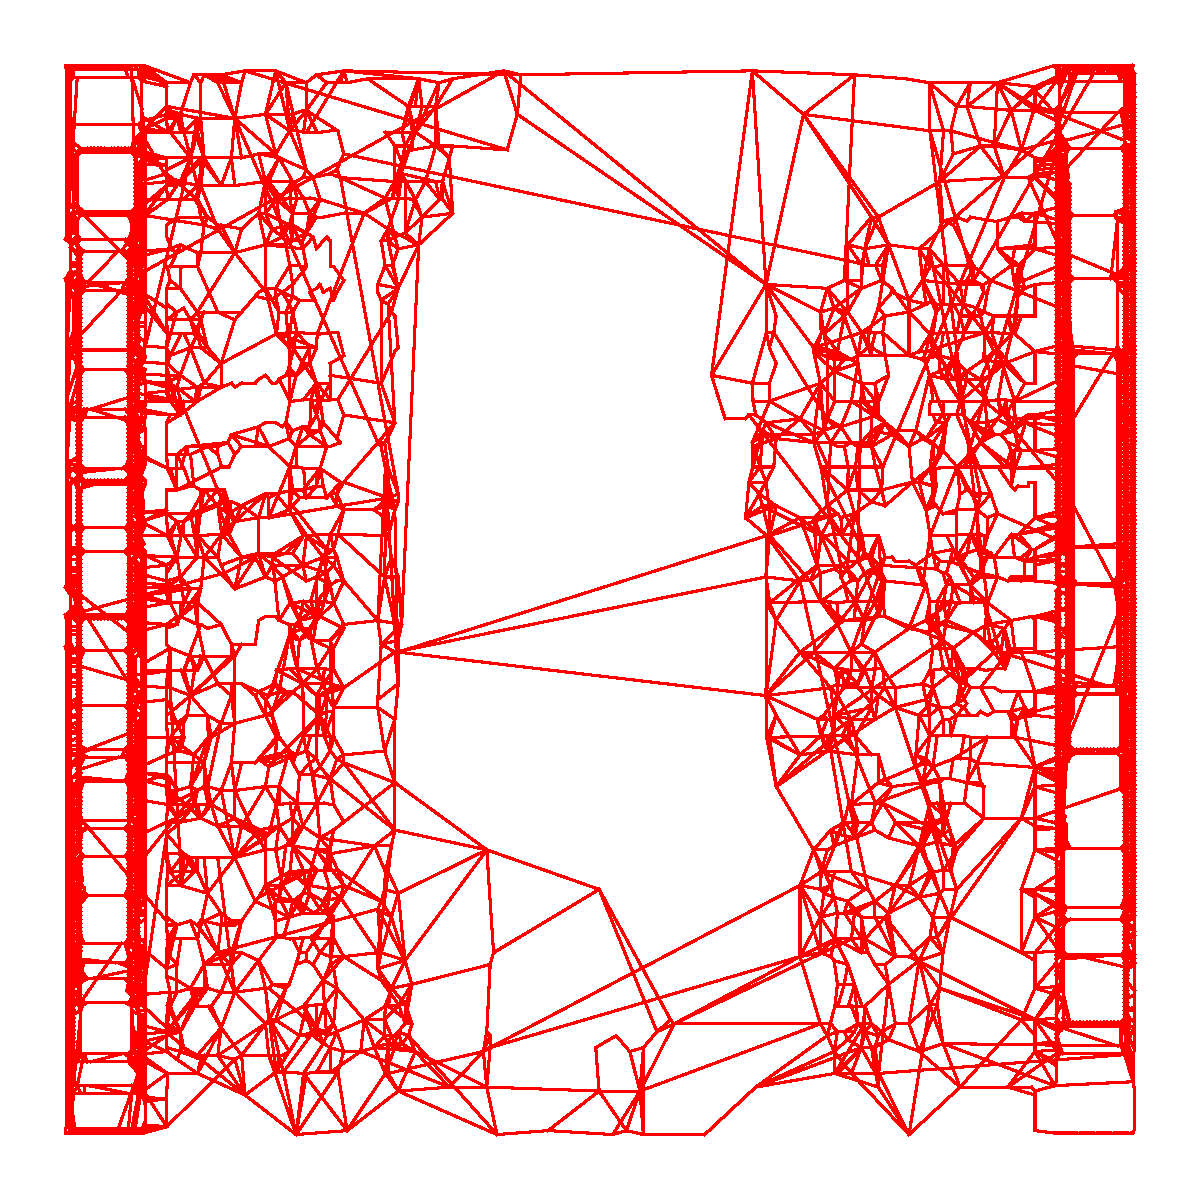
\includegraphics[width=.37\linewidth]{pla7397.0-meNS.pdf}} \qquad
    \subfloat[K-NN]{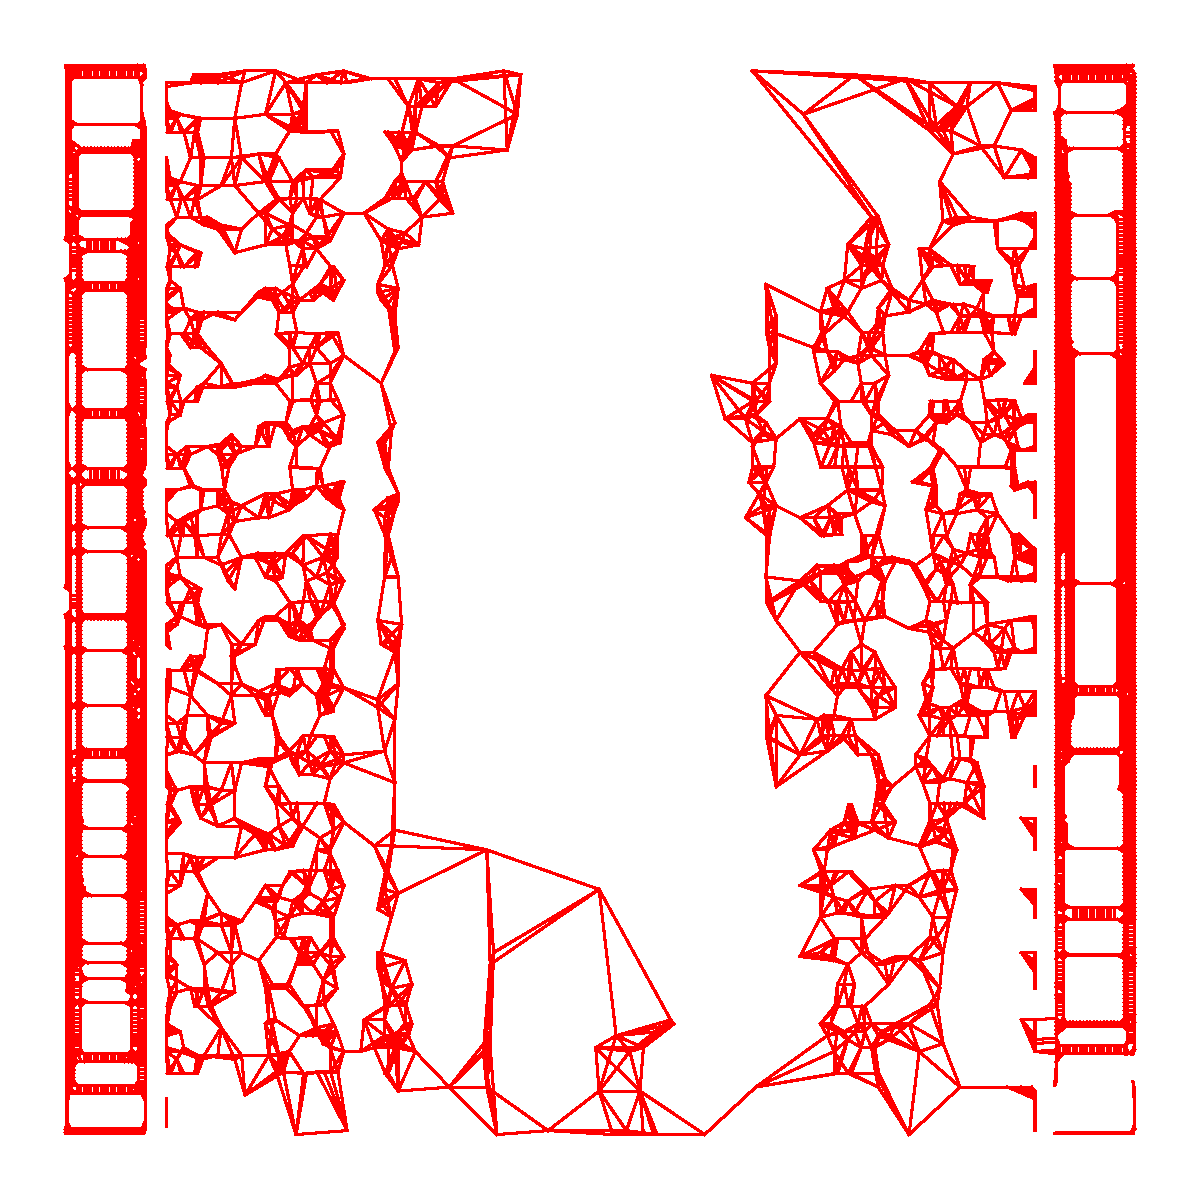
\includegraphics[width=.37\linewidth]{pla7397.0-knNS.pdf}} \\
    \subfloat[$\alpha$-nearest ]{\includegraphics[width=.37\linewidth]{pla7397.0-alNS.pdf}} \qquad
    \subfloat[Delaunay]{\includegraphics[width=.37\linewidth]{pla7397.0-deNS.pdf}}
    \caption[各算法在印刷电路板测试用例$pla7397$生成的邻域结构]{各算法在印刷电路板测试用例$pla7397$生成的邻域结构}
    \label{fig:各算法在印刷电路板测试用例pla7397生成的邻域结构}
\end{figure}
% brd14051
\begin{figure}[!ht]
    \subfloat[meNS]{\includegraphics[width=.37\linewidth]{brd14051.0-meNS.pdf}} \qquad
    \subfloat[K-NN]{\includegraphics[width=.37\linewidth]{brd14051.0-knNS.pdf}} \\
    \subfloat[$\alpha$-nearest ]{\includegraphics[width=.37\linewidth]{brd14051.0-alNS.pdf}} \qquad
    \subfloat[Delaunay]{\includegraphics[width=.37\linewidth]{brd14051.0-deNS.pdf}}
    \caption[各算法在真实地理位置测试用例$brd14051$生成的邻域结构]{各算法在真实地理位置测试用例$brd14051$生成的邻域结构}
    \label{fig:各算法在真实地理位置测试用例brd14051生成的邻域结构}
\end{figure}
\par
从NS Degree指标数据可以知道,虽然meNS生成的邻域结构在修剪后要比其他算法生成的邻域结构在修剪后更加的稀疏,但是这并不意味着meNS的质量会比其他算法的邻域结构的质量要差。从\autoref{tab:各算法表现}~中的最优边遗失率Missing指标数据和LKH最终解的距离趋近度LKH Gap指标数据上可以分析出,在大多数测试用例上,meNS生成的邻域结构在修剪后,其Missing指标值与其他算法生成的邻域结构在修剪后的Missing指标值相差不大,甚至更低,并且在LKH Gap指标数据上,meNS也比其他算法在大多数测试用例上要好。这就意味着,meNS生成算法不仅能够在合理的时间内产生比其他算法更加稀疏的邻域结构,而且在大多数测试用例上,其质量也不比其他算法的邻域结构的质量要低,甚至更好。这从多个方面验证了meNS生成算法的有效性。

\section{本章小结}
\label{sec:NS_Method:本章小结}
本章提出了一种利用最小生成树和欧拉回路来生成邻域结构(meNS)的方法。该算法能够将次梯度优化中产生的未被利用的中间产物1MST,以欧拉回路回路为中间桥梁,构造初始Tour并优化,最后使用这些被优化后的Tour来生成邻域结构。经过实验数据的比较与分析,可以知道meNS生成算法不仅能够在合理的时间内生成比其他算法更加稀疏的邻域结构,而且这些邻域结构能够包含最优Tour中的边,不少于其他算法生成的邻域结构,这意味着meNS生成算法生成的邻域结构更加稀疏的同时,其质量也不比其他算法生成的邻域结构差。

\chapter{基于邻域结构迁移的多目标旅行商问题求解算法}
\label{chap:NST}

\section{引言}
\label{sec:NST:引言}
很多现实中的问题都是由相互冲突和影响的多个目标组成,并且在给定条件下,问题的多个目标需要同时达到最佳,这类问题被称作MOP。当问题的变量域为有限集合时,这类问题就可以被称为CMOP。MOTSP是具有多个冲突的目标的CMOP,并且在大部分行业都可见,包括但不限于交通运输、网络通信和钻孔电路板等领域。由于其变量域所演变出的组合数巨大(NP难),传统的确定性算法难以在一定时间内给出这类问题的解决方案。因此,设计能够在合理时间内给出近似解决方案的启发式方法,就成了求解这类问题的关键。
\par
自多目标组合优化被提出后,研究者们就针对CMOP设计了一系列的MOEA,其大多数是基于EA,可主要分为三大类:基于Pareto支配关系的MOEA\cite{zitzler1999multiobjective,deb2002fast,knowles2000approximating,yang2013grid,laumanns2002combining,hadka2013borg,le2009improved,aguirre2010hybrid,aguirre2013adaptive}、基于指标的MOEA\cite{zitzler2004indicator,bringmann2011approximation,brockhoff20152,rudolph2013evenly,beume2007sms,wagner2007pareto}和基于分解的MOEA\cite{zhang2007moea,zhang2009performance,li2014evolutionary,cheng2016reference,cai2016decomposition,yuan2015balancing}。但是,在应对某些高维度的CMOP,基于Pareto支配关系和基于指标的MOEA都有着其本身的缺陷处。因为在高维度解集中,包含的几乎都是非支配的解,这就导致了只用Pareto支配关系无法区分这些非支配解的优劣,从而不能够均匀且广泛的选出下一代进化的种群。同样,基于指标的MOEA因其指标算法的高复杂度,使得它们在高维度问题中会耗费大量计算资源。然而,基于分解的MOEA因其分解的策略,使得它们被广泛的应用于CMOP中,这使得这种基于分解的方法在过去的十几年中,成为了处理CMOP的最突出的方法之一。一个代表性的算法是MOEA/D\cite{zhang2007moea},其核心思想就是把一个CMOP通过权重向量分解成一组单目标子问题,然后根据各子问题之间的相似度关系构成邻居关系,然后利用邻居子问题之间的信息对所有子问题进行优化。
\par
近年来,利用机器学习中相关的思想来进一步提高MOEA的效率,成为了当下研究的热点。在进化优化的背景下,基于迁移学习(TL)中利用跨问题领域的有用特征数据来提高学习性能这一方法,已经有很多研究者开始将其应用到CMOP当中,并将其与进化算法相结合,提出了进化迁移优化(ETO)\cite{feng2020explicit,lin2020effective,tan2021evolutionary}。在章节~\ref{sec:背景介绍:进化迁移优化}~中可以了解到,在多目标和超多目标优化中的知识信息可以采用非支配解集等形式来实现跨问题的迁移。当ETO与基于分解的MOEA相结合时,分解得来的一系列子问题之间拥有天然的联系,这使得所属子问题的知识能够很好的被迁移到其他子问题上,通过不同子问题之间的相互促进,以此来提高算法的整体效率和质量。
% \par
% 由此,将基于分解的MOEA和ETO相结合,以此来针对CMOP来进行算法设计,是本章研究的重点。由于在ETO中,所使用的知识信息与所求问题密切相关,且本章将使用邻域结构(章节~\ref{subsec:背景介绍:局部搜索:邻域结构})当做被迁移的知识,为此,本章将使用MOTSP问题(章节~\ref{subsec:背景介绍:测试问题:MOTSP})来对设计的算法进行性能测试。

\section{研究动机}
\label{sec:NST:研究动机}
从前面的章节可以了解到,基于分解的MOEA是通过将CMOP分解成一组单目标优化问题,然后对这些单目标问题进行求解,其目的在于将复杂的问题降维,由复杂的CMOP转变成简单的单目标问题,然后可以用解决单目标问题的方法来求解,最后将这些解组合起来就成为了CMOP的解集。并且,在基于分解的方法中最具代表性的MOEA/D中使用了“邻居”的概念,MOEA/D根据被分解后的子问题之间的联系,从而形成子问题间的邻居关系,然后利用子问题之间的联系,通过用当前子问题中的优质解来替换其他邻居子问题中的差解,以此达到不同子问题间的协作效应。
\par
当求解的问题的目标数少时,被分解成的一组单目标优化问题之间存在着“邻居”关系,此时邻居子问题之间还能够依靠着协作来达到相互促进的效果。但是,当求解的问题的目标数变多时,如果依照低维问题的分解粒度,则通过分解得到的单目标问题数量是成指数增加的,这就导致了分解空间的爆炸,若使用算法对如此多的子问题进行优化,这将耗费大量计算资源。如果加大分解的粒度来使得分解得到的子问题恒定,那么这些子问题之间的“邻居”关系将会变得极其微弱,就算当前子问题产生了优质解也难以替换其他子问题的解,这就导致算法的协作效应难以发挥作用。
\par
在进化优化的背景下,ETO利用跨问题领域的知识迁移这一特征能够很好地适用于基于分解的MOEA。因此,可以将ETO的思想融入到基于分解的MOEA当中,在分解得到的子问题之间建立知识迁移模型。因此,使用ETO的目的在于挖掘子问题的内在信息,然后通过迁移的方式将这些信息在不同子问题之间传递使用。然而,通过章节~\ref{sec:背景介绍:进化迁移优化}~可知,现在将ETO应用到CMOP中,大多数是通过将非支配解当做被迁移的信息。然而,通过解迁移的方式,类似于MOEA/D中的协作,如果子问题之间的相似度较低,那么从这些非支配解中能够学习到的有用信息就会很少(解中蕴含的信息本身就少),这些信息很大可能对其他子问题无效,以致产生负迁移,使得难以对问题的优化起到促进作用。
\par
从章节~\ref{subsec:背景介绍:局部搜索:邻域结构}~可以知道,MOTSP可以用邻域结构的方式具现化,这些邻域结构本身就携带了这个问题的大部分特征,并且,邻域结构还能够作为局部搜索算子的一部分。若使用邻域结构来承载子问题的内在信息,容易知道,邻域结构能够承载的信息量要比使用非支配解所蕴含的信息量更多。因此,当以邻域结构作为知识迁移的基本单位,那么就算子问题的相关性变弱,算法也能够从邻域结构中挖掘出一种结构模式,然后使用特定的局部搜索方法来使用该结构,从而促进子问题的优化。
\par
因此,综合章节~\ref{sec:NS_Method:邻域结构生成算法}~提出的邻域结构生成方法,结合基于分解的MOEA和ETO,本章提出了一种基于邻域结构迁移的多目标旅行商问题求解算法(NST-MOEA)。

\section{邻域结构迁移}
\label{sec:NST:邻域结构迁移}
进化迁移优化(ETO)是利用跨问题领域的知识来提高其优化能力的一种方法。容易知道,知识的表达形式,及其如何跨问题迁移是设计算法时的关键点。在提出的邻域结构迁移这一模型中,本章将问题的邻域结构具象化,将邻域结构作为知识迁移的基础单位,视分解得到的多个子问题为不同的问题领域,并且提出了一种由知识关联到问题的两目标相似度模型,该模型能够为每个子问题构造一个知识库,然后使用多臂老虎机模型来获取知识库中的知识,以此达到知识在不同子问题间迁移。

\subsection{子问题}
\label{subsec:NST:邻域结构迁移:子问题}
将CMOP分解成多个子问题的方法有很多,如同章节~\ref{subsec:背景介绍:多目标组合优化算法:基于分解的多目标进化算法}~中介绍的加权和法、切比雪夫法和基于惩罚的边界交叉法。这些分解方法的实质其实是通过聚合的方式,使得CMOP的解的多个维度聚合成一个维度,从而转变为单目标问题。在本章中将提供另外一个分解思路,在对CMOP优化前,就通过权重将该问题分解成不同的子问题,在对问题优化时,每个子问题的解都是单维度的,如若需要可以通过权重将子问题单维度的解还原成多维度的解。
\par
以MOTSP(章节~\ref{subsec:背景介绍:测试问题:MOTSP})为例,给定一组权重向量$\lambda$,有:
\begin{align}
    \label{eq:NST:权重向量}
    & \lambda = \{ \lambda^1, \cdots, \lambda^N \}, \\
    s.t. \quad & \lambda^{i} = [ \lambda^{i}_1, \cdots, \lambda^{i}_m ]^T, \notag \\
    & \forall \lambda^{i}_j \geq 0, \ \sum_{j=1}^m \lambda^{i}_j = 1. \notag
\end{align}
其中,$N$为子问题数,$m$为多目标问题的目标个数,$\lambda^{i}$代表第$i$个子问题的权重向量。假设有一个$m$目标的MOTSP问题$G = (V, E, W)$,其中$V = \{v_1, \cdots, v_n\}$为具有$n$个元素的点集,$E = \{ e_{i,j} = (v_i, v_j) \ | \ v_i, v_j \in V, i \not = j \}$为具有$n(n-1)$个元素的边集,$W$为问题的$m$个边权集,则有:
\begin{align}
    \label{eq:NST:边权矩阵}
    & W = \{ W^1, \cdots, W^m \}, \\
    s.t. \quad & W^k = \{ w^k_{i,j} \ | \ e_{i,j} \in E, i \not = j \}. \notag
\end{align}
其中$W^k$代表第$k$个目标的边权集,$w^k_{i,j}$为边$e_{i,j}$在第$k$个目标上的边权值。则由权重$\mu$对MOTSP问题进行分解,可以得到$N$个子问题$\mathcal{G}$,以$\mathcal{W}$代表这些子问题的边权集,则第$i$个子问题的边权集$\mathcal{W}^i$可以表示为:
\begin{align}
    \label{eq:NST:SP}
    \mathcal{W}^i = \sum_{k=1}^m  \lambda^{i}_k W^i.
\end{align}
容易知道,这些子问题都是单目标的TSP问题,第$i$个子问题可以表示为$\mathcal{G}^i = (V, E, \mathcal{W}^i)$。

\subsection{邻域结构}
\label{subsec:NST:邻域结构迁移:邻域结构}
由章节~\ref{subsec:背景介绍:局部搜索:邻域结构}~可以知道,邻域结构是建立在具体问题的基础之上的。对于TSP问题而言,其邻域结构就是每个顶点只与少数几个顶点相连的稀疏图,该稀疏图也可称为候选集。经由上一节对子问题的介绍可知,当MOTSP问题通过权重向量分解成一组子问题的时,这些子问题其实就是单目标的TSP问题。在本章节中,邻域结构不仅是作为局部搜索的核心结构,同时也是知识迁移的基本单位。所以,在算法中需要在邻域结构和子问题之间建立其映射关系,并将邻域结构也形式化。所以,本节将子问题$\mathcal{G}^k= (V, E, \mathcal{W}^k)$的邻域结构的数学形式表述如下:
\begin{align}
    \label{eq:NST:邻域结构}
    \mathcal{N}^{k} & = \{ \mathcal{N}^{k}_{v_1}, \cdots, \mathcal{N}^{k}_{v_n} \},  \\
    s.t. \quad \mathcal{N}^{k}_{v_i} & = \{ v_1, \cdots, v_j \}, \notag \\
    e_{i,j} & = (v_i,v_j) \in E, \ v_i,v_j \in V, \notag \\
    % & \{ e_{i,1} = (e_i,v_1), \cdots, e_{i,j} = (e_i,v_j) \} \subseteq E, \notag \\
    i,j & \in \{1, \cdots, n\}. \notag
\end{align}
其中,$\mathcal{N}^{k}$为第$k$个子问题的邻域结构,$\mathcal{N}^{k}_{v_i} = \{ v_1, \cdots, v_j \}$为第$k$个子问题中顶点$v_i$的邻域集合,集合中包含$j$个候选点,易知$2 \leq j \leq M$,即邻域集合最少包含$2$个候选点,最多包含$M$个候选点,$M$为邻域修剪时最多能保留的边数。
\par
在章节~\ref{sec:NS_Method:邻域结构生成算法}~中提出了meNS生成方法。在本章中,将使用meNS生成方法为所有子问题生成对应的邻域结构,且以每个点最多保留$M=5$条边的稀疏度来对生成的邻域结构进行修剪。所以,子问题$\mathcal{G}^k = (V, E, \mathcal{W}^k)$的邻域结构为:
\begin{align}
    \label{eq:NST:meNS}
    \mathcal{N}^{k} \xleftarrow[M]{meNS} \mathcal{W}^k.
\end{align}

\subsection{两目标相似度模型}
\label{subsec:NST:邻域结构迁移:两目标相似度模型}
进化迁移优化(ETO)作为近年来较为新颖的方法,在多目标优化领域中,常与其他优化算法相结合的形式在多任务优化当中出现\cite{feng2020explicit,lin2020effective,gupta2016multiobjective}。并且,ETO在多任务优化中具有几个特征:
\begin{itemize}
    \item 任务与任务之间存在相关性,即任务之间具有一定的相似度。
    \item 有知识信息通过任务之间的关联在不同任务之间迁移。
\end{itemize}
其目的在于,使得信息能够在多任务之间进行正迁移,以致于这些信息能够给其它相异的任务起到促进的作用。同理,这些特征在多目标组合优化之中同样适用,当一个多目标组合优化问题分解为多个不同的子问题时,这些子问题之间自然地具有内在的相似性,并且用meNS生成算法为这些子问题生成各自的邻域结构,以这些邻域结构当作信息的载体,然后通过子问题之间的关联来进行邻域结构的迁移,以此达到子问题之间的相互促进。
\par
为了建立子问题和邻域结构之间的映射关系、定量的表示子问题之间的相关性以及邻域结构中所蕴含信息量的多少,下面将介绍两目标相似度模型中关联子问题和邻域结构的两个目标的相关定义。
\par
\begin{definition}
    \label{def:Similarity}
    假设有问题$G = (V,E,W)$,分解向量集$\lambda = \{ \lambda^1, \cdots, \lambda^N \}$,则可得子问题集$\mathcal{G} = \{ \mathcal{G}^1, \cdots , \mathcal{G}^N \}$,如果有子问题$\mathcal{G}^j$和参考子问题$\mathcal{G}^i$,则子问题$\mathcal{G}^j$和参考子问题$\mathcal{G}^i$之间的相似度为两子问题对应的分解权重向量$\lambda^i$与$\lambda^j$之差的$L_2$范数,其数学形式如下:
    \begin{align}
        \label{eq:Similarity}
        & S^i_j  = \|\lambda^j - \lambda^i\|_2, \\
        s.t. \quad & \lambda^i, \lambda^j \in \lambda, \notag \\
        & i,j \in \{1, \cdots, N\}. \notag
    \end{align}
    其中,$\| \cdot \|_2 = \sqrt{\sum \cdot^2}$为$L_2$范数计算公式。由\autoref{eq:Similarity}~可知,子问题和参考子问题之间的相似度实质就是两个子问题所对应分解向量之间的距离,当两子问题之间的差异大,则问题所对应的分解向量的距离就会大,相似度就会小,反之亦然。
\end{definition}
\begin{definition}
    \label{def:Information Gain}
    假设有子问题集$\mathcal{G} = \{ \mathcal{G}^1, \cdots , \mathcal{G}^N \}$,可得对应的邻域结构集$\mathcal{N} = \{ \mathcal{N}^1, \cdots , \mathcal{N}^N \}$,如果有邻域结构$\mathcal{N}^j$和参考邻域结构$\mathcal{N}^i$,则邻域结构$\mathcal{N}^j$相对于参考邻域结构$\mathcal{N}^i$的信息增益为邻域结构$\mathcal{N}^j$中不属于$\mathcal{N}^i$中的候选边的比例,其数学形式如下:
    \begin{align}
        \label{eq:Information Gain}
        & IG^i_j =  \frac{\sum_{\mathcal{N}^j_k \in \mathcal{N}^j} \sum_{\mathcal{N}^j_{k,l} \in \mathcal{N}^j_k} I_{\mathcal{N}_k^i} (\mathcal{N}_{k,l}^j)}{\sum_{\mathcal{N}^j_k \in \mathcal{N}^j} |\mathcal{N}^j_k|}, \\
        s.t. \quad & \mathcal{N}^i, \ \mathcal{N}^j \in \mathcal{N}, \notag  \\
                   & i,j \in \{ 1, \cdots, N \}. \notag
    \end{align}
    其中,$|\cdot|$表示集合中元素的个数,$\mathcal{N}^i_k$是邻域结构$\mathcal{N}^i$中第$k$个点的邻域点集合,则$\mathcal{N}^i_{k,l}$是邻域结构$\mathcal{N}^i$中第$k$个点的第$l$个邻域点,$I_{\mathcal{N}_k^i} (\mathcal{N}_{k,l}^j)$为示性函数,用于判断元素$\mathcal{N}_{k,l}^j$是否属于集合$\mathcal{N}_k^i$,其数学表达式如下:
    \begin{align}
        \label{eq:示性函数}
        I_{\mathcal{N}_k^i} (\mathcal{N}_{k,l}^j) = 
        \begin{cases}
            1, & \mathcal{N}_{k,l}^j \in \mathcal{N}_k^i,     \\
            0, & \mathcal{N}_{k,l}^j \not \in \mathcal{N}_k^i.
        \end{cases}
    \end{align}
\end{definition}
\begin{definition}
    \label{def:Reference Subproblem}
    对于一个具有$m$个目标的CMOP,分解得到中心子问题的权重被定义为$\left[ \frac{1}{m}, \cdots, \frac{1}{m} \right]_{1 \times m} $。则参考子问题被定义为离中心子问题最近的子问题:
    \begin{align}
        \label{eq:Reference Subproblem}
        i = \arg\min_j(|| \lambda^j - [\frac{1}{m},\cdots,\frac{1}{m}]_{1 \times m} ||_2), \ j \in \{1,\cdots,n\}.
    \end{align}
    其中,$i$即为参考子问题在所有子问题中的索引,$n$为子问题的个数。
\end{definition}
则两目标相似度模型的两个目标可定义如下:
\begin{enumerate}
    \item 第一个目标是最小化子问题相对于参考子问题的相似度(\autoref{def:Similarity}):
    \begin{align}\label{eq:First objective}
        minimize \quad & f_1(j) = \mathit{S}^i_j,  \\
        s.t. \quad & j \in \{1, \cdots. n\}. \notag
    \end{align}
    其中,$i$为参考子问题的索引,$n$为子问题的个数。
    \item 第二个目标是最大化子问题的邻域结构相对于参考子问题的邻域结构的信息增益(\autoref{def:Information Gain}):\begin{align}\label{eq:Second objective}
        maximize \quad & f_2(j) = IG^i_j,  \\
        s.t. \quad & j \in \{1, \cdots. n\}. \notag
    \end{align}
    其中,$i$为参考子问题的索引,$n$为子问题的个数。
\end{enumerate}

% \begin{enumerate}
%     \item 第一个目标为相似度:假设有问题$G = (V,E,W)$,分解向量集$\lambda = \{ \lambda^1, \cdots, \lambda^N \}$,则可得子问题集$\mathcal{G} = \{ \mathcal{G}^1, \cdots , \mathcal{G}^N \}$,如果有子问题$\mathcal{G}^j$和参考子问题$\mathcal{G}^i$,则子问题$\mathcal{G}^j$和参考子问题$\mathcal{G}^i$之间的相似度为两子问题对应的分解权重向量$\lambda^i$与$\lambda^j$之差的$L_2$范数,其数学形式如下:
%     \begin{align}
%         \label{eq:Similarity}
%         & S^i_j  = \|\lambda^j - \lambda^i\|_2, \\
%         s.t. \quad & \lambda^i, \lambda^j \in \lambda, \notag \\
%         & i,j \in \{1, \cdots, N\}. \notag
%     \end{align}
%     其中,$\| \cdot \|_2 = \sqrt{\sum \cdot^2}$为$L_2$范数计算公式。由\autoref{eq:Similarity}~可知,子问题和参考子问题之间的相似度实质就是两个子问题所对应分解向量之间的距离,当两子问题之间的差异大,则问题所对应的分解向量的距离就会大,相似度就会小,反之亦然。
%     \item 第二个目标是信息增益(Information Gain,IG):假设有子问题集$\mathcal{G} = \{ \mathcal{G}^1, \cdots , \mathcal{G}^N \}$,可得对应的邻域结构集$\mathcal{N} = \{ \mathcal{N}^1, \cdots , \mathcal{N}^N \}$,如果有邻域结构$\mathcal{N}^j$和参考邻域结构$\mathcal{N}^i$,则邻域结构$\mathcal{N}^j$相对于参考邻域结构$\mathcal{N}^i$的信息增益为邻域结构$\mathcal{N}^j$中不属于$\mathcal{N}^i$中的候选边的比例,其数学形式如下:
%     \begin{align}
%         \label{eq:Information Gain}
%         & IG^i_j =  \frac{\sum_{\mathcal{N}^j_k \in \mathcal{N}^j} \sum_{\mathcal{N}^j_{k,l} \in \mathcal{N}^j_k} I_{\mathcal{N}_k^i} (\mathcal{N}_{k,l}^j)}{\sum_{\mathcal{N}^j_k \in \mathcal{N}^j} |\mathcal{N}^j_k|}, \\
%         s.t. \quad & \mathcal{N}^i, \ \mathcal{N}^j \in \mathcal{N}, \notag  \\
%                    & i,j \in \{ 1, \cdots, N \}. \notag
%     \end{align}
%     其中,$|\cdot|$表示集合中元素的个数,$\mathcal{N}^i_k$是邻域结构$\mathcal{N}^i$中第$k$个点的邻域点集合,则$\mathcal{N}^i_{k,l}$是邻域结构$\mathcal{N}^i$中第$k$个点的第$l$个邻域点,$I_{\mathcal{N}_k^i} (\mathcal{N}_{k,l}^j)$为示性函数,用于判断元素$\mathcal{N}_{k,l}^j$是否属于集合$\mathcal{N}_k^i$,其数学表达式如下:
%     \begin{align}
%         \label{eq:示性函数}
%         I_{\mathcal{N}_k^i} (\mathcal{N}_{k,l}^j) = 
%         \begin{cases}
%             1, & \mathcal{N}_{k,l}^j \in \mathcal{N}_k^i,     \\
%             0, & \mathcal{N}_{k,l}^j \not \in \mathcal{N}_k^i.
%         \end{cases}
%     \end{align}
% \end{enumerate}
\par
从\autoref{eq:First objective}~和\autoref{eq:Second objective}~可知,用相似度来描述子问题之间的关联强弱,能够定量的表示子问题之间的关系。用信息增益来表示邻域结构之间的信息差异,能够定量的表示邻域结构所蕴含的相对信息量。从章节~\ref{sec:NS_Method:实验与讨论}~可以看出,邻域结构能够侧面反映子问题所蕴含的信息,问题的邻域结构的质量能够一定程度上决定最终解的质量,因此,可以将一个问题抽象出一个邻域结构。综上原因易知,不同子问题之间的相似度与其对应的邻域结构之间的信息增益也存在相关性,若两个子问题相似度高,则其对应的邻域结构之间的信息增益也会小,若两个子问题不相关,则它们的邻域结构之间就拥有最大的信息增益。因此,在相似度和信息增益之间存在着映射关系:
\begin{align}
    \label{eq:相似度与信息增益的映射关系}
    f: \ f_1 \mapsto f_2
\end{align}
\par
在建立起子问题和邻域结构的映射关系的基础上,需要为每一个子问题构建一个邻域结构集合用来存放能够被用作迁移的邻域结构,并且要求所子问题所属的邻域结构相对于该子问题的邻域结构在尽可能相似的情形下,能够有尽可能大的信息增益。因为子问题之间越相似,则说明它们的邻域结构也越相似,这使得它们能够互相使用对方的邻域结构。但是子问题之间越相似,其邻域结构之间的信息增益就越小,信息量小则难以对其他子问题起到促进作用。为此,需要找到一个相似度和信息增益之间的平衡,其最终目的在于找到一个合适的相似度,使得构建的邻域结构集合中的邻域结构能够尽可能地产生正迁移。
\par
如\autoref{fig:相似度和信息增益映射关系示意图}~所示是归一化后的相似度和信息增益映射关系示意图。\autoref{eq:获取合适的相似度}~展示的是图中对应的表达式。通过拟合第一个目标(相似度)和第二个目标(信息增益)的映射关系$f_2 = f(f_1)$来求出$f_2$随着$f_1$增加的比率$g$,然后将比率$g$的最大增量$max \ \Delta g$所处的相似度作为为最优相似度$S^*$:
\begin{align}
    \label{eq:获取合适的相似度}
    &f_2 = f(f_1), \\
    &g = f_2', \notag \\
    &\Delta g = g', \notag \\
    &S^* = \arg\max_{f_1} (\Delta g).  \notag
\end{align}
\begin{figure}[htb]
    \includegraphics[width=.7\linewidth]{Kns-KroAB300.pdf}
    \caption[相似度和信息增益映射关系示意图]{相似度和信息增益映射关系示意图}
    \label{fig:相似度和信息增益映射关系示意图}
\end{figure}
\par
通过\autoref{eq:获取合适的相似度}~获取的最优相似度$S^*$,可以为每一个子问题构建一个邻域结构集合用来存放能够被用作迁移的邻域结构。因此,两目标相似度模型的整体流程如算法~\ref{alg:两目标相似度模型}~所示
\begin{algorithm}[!h]
    \caption{两目标相似度模型(Bi-objective Similarity Model,BSM)}
    \label{alg:两目标相似度模型}
    \BlankLine
    \KwIn{ \\
    \hspace{1.1em} $\lambda$:分解权重向量集合 \\
        \hspace{1.1em} $\mathcal{N}$: $n$个子问题的邻域结构; \\
    }
    \KwOut{ \\
        \hspace{1.1em} $NS \ $:邻域结构集合 \\
        \hspace{1.1em} $B \ $:邻居子问题集合
    }
    \tcp{使用分解权重向量集合和所有子问题的邻域结构获取合适的相似度}
    $S^* \xleftarrow[]{\text{式}\eqref{eq:获取合适的相似度}} \lambda, \ \mathcal{N}$ \;
    $NS = \varnothing$ \;
    $B = \varnothing$ \;
    \For{$i=1 \ $ to $ \ n$}{
        $S^i \xleftarrow[]{\text{式}\eqref{eq:Similarity}} \lambda^i, \ \mathcal{N}^i$ \;
        $NS^i = NS^i \bigcup \{ i \} \bigcup \{ j \ | \  S^i_j==S^*, S^i_j \in S^i \}$ \;
        $B^i = B^i \bigcup \{ i \} \bigcup \{ j \ | \  S^i_j \leq S^*, S^i_j \in S^i \}$ \;
    }
    \textbf{return } $NS, \ B$ \;
\end{algorithm}
\par
在算法~\ref{alg:两目标相似度模型}~中,$NS$就是邻域结构集合,$B$是邻居子问题集合。其中,$NS^i$中存储着与第$i$个子问题相似度为0和相似度为$S^*$的子问题的邻域结构的索引,$B^i$中存储着与第$i$个子问题相似度小于或等于$S^*$的子问题的索引。

\subsection{多臂老虎机模型}
\label{subsec:NST:邻域结构迁移:多臂老虎机模型}
多臂老虎机(Multi-armed Bandit,MAB)问题由Robbins于1952年研究统计学时提出\cite{robbins1952some},此后被广泛应用于模拟自动化代理所面临的权衡,该代理旨在通过探索其环境和利用其当前可靠的知识来获得最高的预期收益\cite{kuleshov2014algorithms}。最常见的一个例子:当一个赌徒在面对一台拥有多个拉杆的老虎机时,拉动每一个拉杆都会获得一定的回报奖励(满足一定的概率分布),这个回报奖励和拉杆的分布有关,而赌徒的目的就是在不知道这些拉杆的回报奖励的情况下,最大化自己的收益,且每次只能拉动其中一个拉杆,当赌徒对其中一个拉杆的拉动达到一定的次数时,那么就可以得出这个拉杆的回报奖励对应的统计分布,同时,当赌徒只拉动其中一个或几个拉杆时,那么其他拉杆的拉动次数就会相应的减少,而这些拉杆也有可能会得到更高的回报奖励\cite{曹修山2018基于}。因此,赌徒所面临的问题是:选择已知回报奖励均值最高的拉杆还是选择其他未知但可能获得更好的回报奖励的拉杆\cite{曹修山2018基于,gittins1979bandit}。
\par
在章节~\ref{subsec:NST:邻域结构迁移:两目标相似度模型}~中,两目标相似度模型为算法确定了一个邻域结构库,其中包含了对于相应子问题能够用于知识迁移的邻域结构。但是,在算法中,每次只能选择一个邻域结构用于对当前子问题进行局部搜索。在算法初期,我们不知道哪个邻域结构能为当前子问题带来收益(问题改进),但是我们又期望最终能够获得最大的回报奖励。这正是MAB模型中赌徒遇到的问题。因此,将邻域结构的选择问题建模成一个MAB模型,然后用求解多MAB问题的相关算法来对邻域结构进行选择。
\par
MAB模型中的$\epsilon$-greedy算法\cite{cesa1998finite,vermorel2005multi}、Pursuit算法\cite{thathachar1984class,sutton2018reinforcement}和上置信界(Upper Confidence Bound,UCB)算法\cite{auer2002using,garivier2008upper,slivkins2011contextual}等都能够有效地解决该模型中的利用和探索的权衡问题。因此利用MAB模型中的UCB算法来有效解决在没有先验知识的情况下来选择合适的邻域结构的问题。
\par
上置信界(Upper Confidence Bound,UCB)系列算法由Auer提出\cite{auer2002using},用于解决解决优化问题中的不确定问题。在本节中,给出最简单的UCB算法UCB1。该算法在执行时,会记录每一个邻域结构被选择的次数和回报奖励的均值:
\vspace{-1em}
\begin{align}
    \label{eq:MAB Model}
    M^i &= (t^i, \mu^i), \ i \in \{ 1, \cdots, n \}, \\
    t^i &= \{t^i_j \ | \ j \in \{1,\cdots,\kappa^i\} \}, \notag \\
    \mu^i &= \{\mu^i_j \ | \ j \in \{1,\cdots,\kappa^i\} \}. \notag
\end{align}
其中,$\kappa^i$为第$i$个子问题的邻域结构库中元素的个数,$M^i$就代表了第$i$个子问题记录的参数,$t^i_j$和$\mu^i_j$分别保存着第$i$个子问题中第$j$个邻域结构被选择的次数和回报奖励的均值。算法在初始时将每一个邻域结构都使用一次,在之后的第$t$轮中,算法会根据以下公式来选择第$i$个子问题的邻域结构:
\begin{align}
    \label{eq:UCB}
    UCB_{M^i}(t) = argmax_{j=1,\cdots,\kappa^i}(\mu^i_j + \sqrt{\frac{2\log(t)}{t^i_j}}).
\end{align}
其中,$\kappa^i$就是第$i$个子问题中邻域结构库中的邻域结构的数目,就相当于MAB模型中拉杆的数量。在每一轮选择后,算法会根据\autoref{eq:Update MAB Model}~更新$M^i$,并且在下一轮中重新选择邻域结构。
\begin{align} \label{eq:Update MAB Model}
    \mu^i_j &= \frac{\mu^i_j*t^i_j+r_{t^i_j+1}}{t^i_j+1}, \\
    t^i_j &= t^i_j + 1. \notag
\end{align}
其中$j$是在第$t$轮选择的邻域结构的索引,$r_{t^i_j+1}$是邻域结构库中第$j$个邻域结构第$(t^i_j+1)$次被选中时的奖励。
\par
\autoref{eq:UCB}~的目的就是根据以往的选择经验,来选择置信度最高的邻域结构。并且,Auer\cite{auer2002using}和Bouneffouf等人\cite{bouneffouf2016multi}证明了,当进行$t$次试验,上置信界算法的遗憾度是有上界的,并且界限为:
\begin{align}
    \label{eq:Regret Bound}
    [8\sum_{i:\mu_i < \mu^*} (\frac{\ln t}{\Delta_i})] + (1 + \frac{\pi^2}{3})(\sum_{j=1}^{\kappa} \Delta_j).
\end{align}
其中,$\Delta_i = \mu^* - \mu_i$。

\section{算法设计}
\label{sec:NST:算法设计}
本节将介绍基于邻域结构迁移的多目标旅行商问题求解算法(NST-MOEA)的设计细节。NST-MOEA总体可分为三个部分:
\begin{enumerate}
    \item 初始化阶段:初始化算法参数,包括对邻域结构迁移中的模型进行初始化。
    \item 局部搜索阶段:对所有子问题进行改进,促使种群进化。
    \item 更新阶段:更新算法的参数,包括邻居子问题的解、邻域结构迁移中的模型参数和外部种群集的更新。
\end{enumerate}
下面将对NST-MOEA的主要算法框架进行介绍,然后分节对NST-MOEA中的各个部分进行描述。

\subsection{NST-MOEA算法主框架}
\label{subsec:NST:算法设计:NST-MOEA算法主框架}
算法~\ref{alg:NST-MOEA算法主框架}~所示的NST-MOEA的算法框架中,维持了在算法中使用的几个全局的属性集合,以下是它们的符号表示及其含义:
\begin{enumerate}
    \item $EP$: 所有非支配解的外部集合;
    \item $\mathcal{N}$: 所有子问题的邻居结构集合;
    \item $\mathcal{NS}$: 所有子问题的邻域结构库集合(存邻域结构的索引);
    \item $B$: 所有子问题的邻居子问题集合(存子问题索引);
    \item $M$: 所有子问题的多臂老虎机模型参数集合。
\end{enumerate}
\par
\begin{algorithm}[!h]
    \caption{NST-MOEA算法主框架}
    \label{alg:NST-MOEA算法主框架}
    \BlankLine
    \KwIn{ \\
        \hspace{1.1em} $Stop$:算法终止条件 \\
        \hspace{1.1em} $W$:多目标组合优化问题的权重集合 \\
        \hspace{1.1em} $\lambda$:分解权重向量集合
    }
    \KwOut{ \\
        \hspace{1.1em} $EP \ $:外部集合
    }
    \tcp{使用邻域结构生成方法为所有子问题生成邻域结构}
    $\mathcal{N} \xleftarrow[]{meNS} W, \ \lambda$ \label{line:meNS} \;
    \tcp{通过两目标相似度模型为每个子问题构造邻域结构集合和邻居子问题}
    [$NS, \ B$] = $BSM(\lambda, \ \mathcal{N})$ \label{line:BSM} \;
    \tcp{根据\autoref{eq:MAB Model},初始化MAB模型参数为0}
    $M = \mathbf{0}$ \label{line:MAB} \;
    \tcp{随机生成初始种群}
    $P = \{x^1, \cdots, x^n\}$ \label{line:初始化P} \;
    $EP = \varnothing$  \label{line:初始化EP}\;
    $t = 0$ \label{line:初始化t} \;
    \While{$t$++ and $!Stop$}{
        \For{$i=1 \ $ to $\ n$}{
            \tcp{通过上置信界算法选择邻域结构}
            $j = UCB_{M^i}(t)$ \label{line:UCB} \;
            \tcp{对个体进行局部搜索}
            $x'$ = LS($x^i$, $\mathcal{N}^{\mathcal{NS}^i_j}$) \label{line:LS} \;
            \tcp{更新参数}
            UPDATE($x^i$, $x'$, $B^i$, $M^i$, $EP$) \label{line:Update} \;
        }
    }
    \textbf{return } $EP$ \;
\end{algorithm}
算法~\ref{alg:NST-MOEA算法主框架}~展示的是NST-MOEA算法主框架,从伪代码也能够看出,算法整体分为了三部分:1)初始化部分(第~\ref{line:meNS}$\thicksim$\ref{line:初始化t}~行);2)局部搜索部分(第~\ref{line:UCB}$\thicksim$\ref{line:LS}~行);3)更新部分(第~\ref{line:Update}~行)。在算法~\ref{alg:NST-MOEA算法主框架}~中,在对算法各参数进行初始化后,就使用局部搜索对种群中的个体进行迭代优化,直到满足算法的终止条件,并且每次对种群中的个体进行优化后,都需要将相应的参数进行更新,最终,算法返回保存非支配解的外部集$EP$。下面将分节详细介绍算法的各个子部分。

\subsection{初始化阶段}
\label{subsec:NST:算法设计:初始化阶段}
在算法~\ref{alg:NST-MOEA算法主框架}~的第~\ref{line:meNS}$\thicksim$\ref{line:初始化t}~行是初始化部分。首先为所有子问题生成邻域结构,本章使用meNS生成方法为子问题生成邻域结构。然后,如算法~\ref{alg:两目标相似度模型}~中所示,使用两目标相似度模型初始化每个子问题的邻域结构集合和邻居子问题。接着通过\autoref{eq:MAB Model}~为每个子问题都建立MAB模型,并初始化参数。最后,在算法~\ref{alg:NST-MOEA算法主框架}~的第~\ref{line:初始化P}~行随机生成初始种群$P$,第~\ref{line:初始化EP}~行和~\ref{line:初始化t}~行分别是设置外部集合$EP$为空集和设置试验轮数$t=0$。

\subsection{局部搜索阶段}
\label{subsec:NST:算法设计:局部搜索阶段}
局部搜索阶段也分为了两部分,第一部分通过上置信界算法(UCB,\autoref{eq:UCB})来对子问题的邻域结构库$\mathcal{NS}$中的邻域结构进行选择。第二步就是使用第一步选择的邻域结构来对子问题进行局部搜索。在本章中使用的局部搜索方法是Lin-Kernighan(LK)算法\cite{lin1973effective},LK算法本质上是一个在巡回路径$T$上进行$k$-opt移动(\autoref{fig:k-opt示意图})的方法,其核心思想就是通过用$k$条不属于$T$的边来替换$T$中的$k$条边,在使得换边后的巡回路径$T$合法的前提下,尽可能的使得$T$被改进优化.若给定一条巡回路径$T = \{t_1, \cdots, t_n\}$和邻域结构$\mathcal{N}$,则LK算法的执行流程如下:
\begin{description}
    \item[步骤1]:设置迭代次数$i=1$;
    \item[步骤2]:从$T$中获取一条边$e_i = \{t_i, t_{i+1}\}$,并且将$e_i$并入到减边集$X$;
    \item[步骤3]:从邻域结构$\mathcal{N}$中,获取边$e_{t_{2i}, t_{2i+1}}, t_{2i+1} \in \mathcal{N}_{t_{i+1}}$,并且将边$e_{t_{2i}, t_{2i+1}}$并入到加边集$Y$;
    \item[步骤4]:迭代次数加1;
    \item[步骤5]:执行\textbf{步骤2},将$e_{t_{1}, t_{2i}}$并入到加边集,在$T$中用$Y$替换$X$得到$T'$,如果$T'$优于$T$,则返回$T'$,否则执行\textbf{步骤3}。
\end{description}

\subsection{更新阶段}
\label{subsec:NST:算法设计:更新阶段}
在算法~\ref{alg:NST-MOEA算法主框架}~的第~\ref{line:Update}~行的更新操作如算法~\ref{alg:UPDATE}~所示。算法~\ref{alg:UPDATE}~主要是对3个集合进行更新。首先是用$x'$对子问题的邻居子问题的解进行更新。然后计算当前轮次获得的收益$r$,然后用收益$r$根据\autoref{eq:Update MAB Model}~对子问题的MAB模型进行更新。最后用$x'$对$EP$集进行更新,主要目的是将$EP$中被$x'$支配的个体排除掉,并且判断是否将$x'$加入到$EP$集中。
\par
\begin{algorithm}[!h]
    \caption{UPDATE}
    \label{alg:UPDATE}
    \BlankLine
    \KwIn{ \\
        \hspace{1.1em} $x^i$: 第$i$个子问题所关联的解 \\
        \hspace{1.1em} $x'$: $x^i$经过局部搜索改进后的解 \\
        \hspace{1.1em} $B^i$: 第$i$个子问题的邻居子问题的索引 \\
        \hspace{1.1em} $M^i$: 第$i$个子问题的MAB模型 \\
        \hspace{1.1em} $EP$: 外部集合
    }
    \tcp{更新子问题的邻居解}
    \ForEach{$j \in B^i)$}{
        \If{对于第$j$个子问题,$x'$优于$x^j$}{
            \tcp{用$x'$替换$x^j$}
            $x^j = x'$ \;
        }
    }
    \tcp{获取本轮的奖励值}
    $r = f(x^i)-f(x')$ \;
    通过\autoref{eq:Update MAB Model}~和奖励$r$更新MAB模型$M^i$ \;
    \tcp{用$x'$更新外部集}
    \ForEach{$x \in EP$}{
        \If{$x' \in x$}{
            \tcp{从$EP$中删除$x$}
            $EP = EP/\{x\}$ \;
        }
    }
    \If{$x \not \prec x', \forall x \in EP$}{
        $EP = EP \bigcup \{x'\}$ \;
    }
\end{algorithm}

\section{实验与讨论}
\label{sec:NST:实验与讨论}

\subsection{测试集}
\label{subsec:NST:实验与讨论:测试集}
本节将采用MOTSP问题(章节~\ref{subsec:背景介绍:测试问题:MOTSP})来对算法进行实验。其测试集包含了TSPLIB\footnote{http://comopt.ifi.uni-heidelberg.de/software/TSPLIB95/}中的部分测试集,包括了“Cluster”、“Euclid”和“Kro”三种类型的测试用例,同时包含了中国三级城镇经纬度坐标\footnote{http://lbsyun.baidu.com/index.php?title=open/dev-res}所生成的真实地理数据测试集(Real)。所有测试用例的节点数在100$\sim$1000之间,目标数在2$\sim$8之间。如\autoref{tab:MOTSP问题测试集}~所示,测试用例被命名为“类型+目标+节点数”的形式,对于测试用例“KroAB100”,代表测试用例的类型为“Kro”,用两个目标“AB”且节点数为100。
\par
\begin{table}[h]
    \small
    \renewcommand\tabcolsep{4.5pt}
    \centering
    \caption{MOTSP问题测试集 \label{tab:MOTSP问题测试集}}
    \begin{threeparttable}
        \begin{tabular}{llcll|llcll}
        \toprule
        测试用例  & 类型 & 目标数   & 节点数   & 权重类型  & 测试用例  & 类型 & 目标数   & 节点数   & 权重类型 \\
        \midrule
        KroAB100 & Kro   & 2     & 100   & EUC\_2D & RealAB100 & Real  & 2     & 100   & GEO \\
        KroAB200 & Kro   & 2     & 200   & EUC\_2D & RealBC100 & Real  & 2     & 100   & GEO \\
        KroAB300 & Kro   & 2     & 300   & EUC\_2D & RealCD100 & Real  & 2     & 100   & GEO \\
        KroAB400 & Kro   & 2     & 400   & EUC\_2D & RealAB300 & Real  & 2     & 300   & GEO \\
        KroAB500 & Kro   & 2     & 500   & EUC\_2D & RealAB500 & Real  & 2     & 500   & GEO \\
        KroAB750 & Kro   & 2     & 750   & EUC\_2D & RealAB750 & Real  & 2     & 750   & GEO \\
        KroAB1000 & Kro   & 2     & 1000  & EUC\_2D & RealAB1000 & Real  & 2     & 1000  & GEO \\
        ClusterAB100 & Cluster & 2     & 100   & EUC\_2D & RealABC100 & Real  & 3     & 100   & GEO \\
        ClusterAB300 & Cluster & 2     & 300   & EUC\_2D & RealBCD100 & Real  & 3     & 100   & GEO \\
        ClusterAB500 & Cluster & 2     & 500   & EUC\_2D & RealCDE100 & Real  & 3     & 100   & GEO \\
        EuclidAB100 & Euclid & 2     & 100   & EUC\_2D & RealA$\sim$D100 & Real  & 4     & 100   & GEO \\
        EuclidAB300 & Euclid & 2     & 300   & EUC\_2D & RealB$\sim$E100 & Real  & 4     & 100   & GEO \\
        EuclidAB500 & Euclid & 2     & 500   & EUC\_2D & RealC$\sim$F100 & Real  & 4     & 100   & GEO \\
        KroABC100 & Kro   & 3     & 100   & EUC\_2D & RealA$\sim$E100 & Real  & 5     & 100   & GEO \\
        KroBCD100 & Kro   & 3     & 100   & EUC\_2D & RealB$\sim$F100 & Real  & 5     & 100   & GEO \\
        KroCDE100 & Kro   & 3     & 100   & EUC\_2D & RealC$\sim$G100 & Real  & 5     & 100   & GEO \\
        KroA$\sim$D100 & Kro   & 4     & 100   & EUC\_2D & RealA$\sim$F100 & Real  & 6     & 100   & GEO \\
        KroB$\sim$E100 & Kro   & 4     & 100   & EUC\_2D & RealB$\sim$G100 & Real  & 6     & 100   & GEO \\
        EuclidA$\sim$D100 & Euclid & 4     & 100   & EUC\_2D & RealC$\sim$H100 & Real  & 6     & 100   & GEO \\
        EuclidB$\sim$E100 & Euclid & 4     & 100   & EUC\_2D & RealA$\sim$G100 & Real  & 7     & 100   & GEO \\
        EuclidC$\sim$F100 & Euclid & 4     & 100   & EUC\_2D & RealB$\sim$H100 & Real  & 7     & 100   & GEO \\
        EuclidD$\sim$G100 & Euclid & 4     & 100   & EUC\_2D & RealC$\sim$I100 & Real  & 7     & 100   & GEO \\
        EuclidE$\sim$H100 & Euclid & 4     & 100   & EUC\_2D & RealA$\sim$H100 & Real  & 8     & 100   & GEO \\
        EuclidA$\sim$E100 & Euclid & 5     & 100   & EUC\_2D & RealB$\sim$I100 & Real  & 8     & 100   & GEO \\
        EuclidB$\sim$F100 & Euclid & 5     & 100   & EUC\_2D & EuclidB$\sim$G100 & Euclid & 6     & 100   & EUC\_2D \\
        EuclidC$\sim$G100 & Euclid & 5     & 100   & EUC\_2D & EuclidC$\sim$H100 & Euclid & 6  & 100   & EUC\_2D  \\
        EuclidD$\sim$H100 & Euclid & 5     & 100   & EUC\_2D & EuclidA$\sim$G100 & Euclid & 7  & 100   & EUC\_2D  \\
        EuclidA$\sim$F100 & Euclid & 6     & 100   & EUC\_2D & EuclidB$\sim$H100 & Euclid & 7  & 100   & EUC\_2D  \\
        \bottomrule
    \end{tabular}
    \begin{tablenotes}
        \item[] “A$\sim$D”代表“ABCD”
    \end{tablenotes}
    \end{threeparttable}
\end{table}
在\autoref{tab:MOTSP问题测试集}~中的测试用例有两种权重类型:TSPLIB中的测试用例的权重类型都为欧几里得距离($EUC\_2D$),其计算公式可参考\autoref{eq:EUC2D};真实地理数据测试用例的权重类型为经纬度距离($GEO$),假设有两点及其经纬度坐标$v_i = (x_i, y_i)$和$v_j = (x_j, y_j)$,$x$为纬度(Latitude),$y$为经度(Longitude),都为浮点数,则其边权$w_{i,j}$计算公式如下:
\vspace{-1em}
\begin{align}
    \label{eq:GEO}
    & w_{i,j} =\lfloor R * \arccos(0.5*((1+q_1)*q_2 - (1-q_1)*q_3)) + 1 \rfloor, \\
    s.t. \quad & R = 6378.388, \notag  \\
    & lat_i, lon_i = Convert(v_i), \ lat_j, lon_j = Convert(v_j), \notag \\
    & q_1 = \cos(lon_i - lon_j), \  q_2 = \cos(lat_i - lat_j), \ q_3 = \cos(lat_i + lat_j). \notag
\end{align}
其中,$Convert$(算法~\ref{alg:浮点数转经纬度})将浮点数坐标转换成经纬度坐标,$R$为地球半径$6378.388$公里。
\begin{algorithm}[!h]
    \caption{浮点数转经纬度(Convert)}
    \label{alg:浮点数转经纬度}
    \BlankLine
    \KwIn{ \\
        \hspace{1.1em} $v = (x, y) \ $: 节点$v$的浮点数坐标 \\
    }
    \KwOut{ \\
        \hspace{1.1em} $lat, lon \ $:节点$v$的经纬度坐标
    }
    \tcp{将浮点数拆分成角度和角分,然后计算经纬度}
    $deg_x = \lfloor x + 0.5 \rfloor$ \;
    $min_x = x - deg_x$ \;
    $lat = (deg_x + \frac{5}{3}min_x)\pi/180$ \;
    $deg_y = \lfloor y + 0.5 \rfloor$ \;
    $min_y = y - deg_y$ \;
    $lot = (deg_y + \frac{5}{3}min_y)\pi/180$ \;
    \textbf{return } $lat, lon$ \;
\end{algorithm}
\par
在\autoref{tab:MOTSP问题测试集}~中的真实地理数据测试集“Real”是根据3074个三级城镇经纬度坐标随机生成的,构造测试集时,随机种子设为$N+m$,其中$N$为要生成的测试问题的节点数量,$m$为测试问题中的目标数。同时,为了测试算法的性能,本节主要用到了超体积度量指标(章节~\ref{subsec:背景介绍:性能评价指标:超体积度量指标})和集合覆盖度量指标(章节~\ref{subsec:背景介绍:性能评价指标:集合覆盖度量指标})。

\subsection{实验参数设置}
\label{subsec:NST:实验与讨论:实验参数设置}
在本章中,会将NST-MOEA与多种其他类型的算法作性能对比,这些算法为MOEA/D(包含WS、TCH和PBI三种分解方式)\cite{zhang2007moea}、DCDG\cite{cai2019collaborative}、GWS-PLS\cite{cai2018grid}和2PPLS\cite{lust2010speed}。下面给出各算法的参数设置和说明:
\begin{itemize}
    \item MOEA/D:包含三种分解方法,其种群大小都为300,子问题的邻居大小设为20,对于PBI分解方法,惩罚因子设为5,最大迭代次数为1000。
    \item DCDG:种群大小为300,网格分割参数L设为10,对于二维目标,网格邻居距离设为5,三维以上设为1,最大迭代次数为700。
    \item GWS-PLS:种群大小为300,对于2、3、4、5、6、7和8目标问题网格划分参数L分别设为200、14、7、5、4、3、2),对于100节点的问题最大迭代次数设为300,200、300和400节点最大迭代次数设为500,500、750和1000节点最大迭代次数设为1000。
    \item 2PLLS:初始解数量为300,最大迭代次数为100,。由于该算法计算量随目标数呈指数级增长\cite{lust2012multiobjective},所以只测试了两个目标的测试用例。
    \item NST-MOEA:种群大小为300,最大迭代次数为($\lfloor (n/100+1)/2 \rfloor * 100$),$n$为问题的节点数。
\end{itemize}
所有算法都是用局部搜索算子(2-opt、3-opt和4-opt(如\autoref{fig:k-opt示意图}))产生新解,当算法没有新解产生或者到达最大迭代次数时终止。所有算法的初始种群都为同一个随机生成的种群,且所有算法在每个测试用例上均独立运行30次。

\subsection{各算法在TSPLIB测试集上的对比}
\label{subsec:NST:实验与讨论:各算法在TSPLIB测试集上的对比}
% TODO: 对比图片重新画,改成中文版
在本节中,将会对NST-MOEA与MOEA/D(WS、TCH和PBI)、DCDG、GWS-PLS和2PPLS算法在TSPLIB测试集上进行对比。\autoref{fig:各算法在KroAB300上的非支配解集示意图}~、\autoref{fig:各算法在KroABC100上的非支配解集示意图}~和\autoref{fig:各算法在KroABCD100上的非支配解集示意图}~分別展示的是TSPLIB中部分测试用例(2、3和4目标)在相同尺度下的的最终非支配集可视化图。
\par
% \begin{figure}[!h]
%     \subfloat[All Algorithms \label{subfig:KroAB300-All Algorithms}]{\includegraphics[width=.5\linewidth]{PF/KroAB300/Thesis-All-SameScale1-PF.pdf}} \qquad
%     \subfloat[NST-MOEA \label{subfig:KroAB300-NST-MOEA}]{\includegraphics[width=.32\linewidth]{PF/KroAB300/Thesis-NST-MOEA-SameScale1-PF.pdf}} 
%     \caption[各算法在KroAB300上的非支配解集示意图]{各算法在KroAB300上的非支配解集示意图}
%     \label{fig:各算法在KroAB300上的非支配解集示意图}
% \end{figure}
% \begin{figure}[t]
%     \ContinuedFloat
%     \subfloat[MOEA/D-WS \label{subfig:KroAB300-MOEA/D-WS}]{\includegraphics[width=.3\linewidth]{PF/KroAB300/Thesis-MOEAD-WS-SameScale1-PF.pdf}} \quad
%     \subfloat[MOEA/D-TCH \label{subfig:KroAB300-MOEA/D-TCH}]{\includegraphics[width=.3\linewidth]{PF/KroAB300/Thesis-MOEAD-TCH-SameScale1-PF.pdf}} \quad
%     \subfloat[MOEA/D-PBI \label{subfig:KroAB300-MOEA/D-PBI}]{\includegraphics[width=.3\linewidth]{PF/KroAB300/Thesis-MOEAD-PBI-SameScale1-PF.pdf}} \\
%     \subfloat[DCDG \label{subfig:KroAB300-DCDG}]{\includegraphics[width=.3\linewidth]{PF/KroAB300/Thesis-DCDG-SameScale1-PF.pdf}} \quad
%     \subfloat[GWS-PLS \label{subfig:KroAB300-GWS-PLS}]{\includegraphics[width=.3\linewidth]{PF/KroAB300/Thesis-GWS-PLS-SameScale1-PF.pdf}} \quad
%     \subfloat[2PPLS \label{subfig:KroAB300-2PPLS}]{\includegraphics[width=.3\linewidth]{PF/KroAB300/Thesis-2PPLS-SameScale1-PF.pdf}}
%     \caption[]{各算法在KroAB300上的非支配解集示意图(续)}
% \end{figure}
\begin{figure}[!h]
    \subfloat[All Algorithms \label{subfig:KroAB300-All Algorithms}]{\includegraphics[width=.5\linewidth]{PF/KroAB300/Thesis-All-SameScale1-PF.pdf}} \qquad
    \subfloat[NST-MOEA \label{subfig:KroAB300-NST-MOEA}]{\includegraphics[width=.32\linewidth]{PF/KroAB300/Thesis-NST-MOEA-SameScale1-PF.pdf}}  \\
    \subfloat[MOEA/D-WS \label{subfig:KroAB300-MOEA/D-WS}]{\includegraphics[width=.3\linewidth]{PF/KroAB300/Thesis-MOEAD-WS-SameScale1-PF.pdf}} \quad
    \subfloat[MOEA/D-TCH \label{subfig:KroAB300-MOEA/D-TCH}]{\includegraphics[width=.3\linewidth]{PF/KroAB300/Thesis-MOEAD-TCH-SameScale1-PF.pdf}} \quad
    \subfloat[MOEA/D-PBI \label{subfig:KroAB300-MOEA/D-PBI}]{\includegraphics[width=.3\linewidth]{PF/KroAB300/Thesis-MOEAD-PBI-SameScale1-PF.pdf}} \\
    \subfloat[DCDG \label{subfig:KroAB300-DCDG}]{\includegraphics[width=.3\linewidth]{PF/KroAB300/Thesis-DCDG-SameScale1-PF.pdf}} \quad
    \subfloat[GWS-PLS \label{subfig:KroAB300-GWS-PLS}]{\includegraphics[width=.3\linewidth]{PF/KroAB300/Thesis-GWS-PLS-SameScale1-PF.pdf}} \quad
    \subfloat[2PPLS \label{subfig:KroAB300-2PPLS}]{\includegraphics[width=.3\linewidth]{PF/KroAB300/Thesis-2PPLS-SameScale1-PF.pdf}}
    \caption[各算法在KroAB300上的非支配解集示意图]{各算法在KroAB300上的非支配解集示意图}
    \label{fig:各算法在KroAB300上的非支配解集示意图}
\end{figure}
\par
从\autoref{fig:各算法在KroAB300上的非支配解集示意图}~可以看出,在二目标测试问题上,MOEA/D-WS得到的非支配解集分布广泛但是不均匀,其PF面有很多缺失的部分。相反,MOEA/D-TCH和MOEA/D-PBI得到的非支配解集分布均匀但是不广泛,丢失了两端边界区域的解,可以看出,子问题不同的分解方式对MOEA/D最终的非支配解集的影响会很大。DCDG获得的非支配解集与MOEA/D-PBI类似,相比于其他算法,它也缺失了两端边界区域的解。从图中还能看出,GWS-PLS、2PPLS和NST-MOEA获得的非支配解集都分布广泛且均匀,但是在最后一个子图的局部放大图中可以看出,NST-MOEA获得的非支配解集的收敛效果比其他算法都好。从\autoref{fig:各算法在KroABC100上的非支配解集示意图}~和\autoref{fig:各算法在KroABCD100上的非支配解集示意图}~可以看出,各算法在高维目标测试问题与二目标测试问题所呈现的非支配解集分布情况相似。除了NST-MOEA获得的非支配解集分布广泛且均匀,MOEA/D-LS获得的解集广泛但不均匀外,其他算法获得的解集都在不同程度上缺失了边界区域的解。并且,结合\autoref{fig:各算法Hypervolume指标对比示意图}~所示的各算法HV指标箱型图,能够知道,NST-MOEA在获得的非支配解集不仅在分布性上表现的要比其他算法好,而且非支配解集的收敛性也要由于其他算法。
\begin{figure}[!h]
    \subfloat[NST-MOEA \label{subfig:KroABC100-NST-MOEA}]{\includegraphics[width=.275\linewidth]{PF/KroABC100/Thesis-NST-MOEA-SameScale1-PF.pdf}} \quad
    \subfloat[MOEA/D-WS \label{subfig:KroABC100-MOEA/D-WS}]{\includegraphics[width=.275\linewidth]{PF/KroABC100/Thesis-MOEAD-WS-SameScale1-PF.pdf}} \quad
    \subfloat[MOEA/D-TCH \label{subfig:KroABC100-MOEA/D-TCH}]{\includegraphics[width=.275\linewidth]{PF/KroABC100/Thesis-MOEAD-TCH-SameScale1-PF.pdf}} \\
    \subfloat[MOEA/D-PBI \label{subfig:KroABC100-MOEA/D-PBI}]{\includegraphics[width=.275\linewidth]{PF/KroABC100/Thesis-MOEAD-PBI-SameScale1-PF.pdf}} \quad
    \subfloat[DCDG \label{subfig:KroABC100-DCDG}]{\includegraphics[width=.275\linewidth]{PF/KroABC100/Thesis-DCDG-SameScale1-PF.pdf}}  \quad
    \subfloat[GWS-PLS \label{subfig:KroABC100-GWS-PLS}]{\includegraphics[width=.275\linewidth]{PF/KroABC100/Thesis-GWS-PLS-SameScale1-PF.pdf}}
    \caption[各算法在KroABC100上的非支配解集示意图]{各算法在KroABC100上的非支配解集示意图}
    \label{fig:各算法在KroABC100上的非支配解集示意图}
\end{figure}
\begin{figure}[!h]
    \subfloat[MOEA/D-WS \label{subfig:KroABCD100-MOEA/D-WS}]{\includegraphics[width=.275\linewidth]{PF/KroABCD100/Thesis-MOEAD-WS-SameScale1-PF.pdf}} \quad
    \subfloat[MOEA/D-TCH \label{subfig:KroABCD100-MOEA/D-TCH}]{\includegraphics[width=.275\linewidth]{PF/KroABCD100/Thesis-MOEAD-TCH-SameScale1-PF.pdf}} \quad
    \subfloat[MOEA/D-PBI \label{subfig:KroABCD100-MOEA/D-PBI}]{\includegraphics[width=.275\linewidth]{PF/KroABCD100/Thesis-MOEAD-PBI-SameScale1-PF.pdf}} \\
    \subfloat[GWS-PLS \label{subfig:KroABCD100-GWS-PLS}]{\includegraphics[width=.275\linewidth]{PF/KroABCD100/Thesis-GWS-PLS-SameScale1-PF.pdf}} \quad
    \subfloat[NST-MOEA \label{subfig:KroABCD100-NST-MOEA}]{\includegraphics[width=.275\linewidth]{PF/KroABCD100/Thesis-NST-MOEA-SameScale1-PF.pdf}}
    \caption[各算法在KroABCD100上的非支配解集示意图]{各算法在KroABCD100上的非支配解集示意图}
    \label{fig:各算法在KroABCD100上的非支配解集示意图}
\end{figure}
\begin{figure}[!h]
    \subfloat[KroAB100 \label{subfig:Box-HV-kroAB100}]{\includegraphics[width=.4\linewidth]{Box-HV-KroAB100.pdf}} \quad
    \subfloat[KroAB300 \label{subfig:Box-HV-kroAB300}]{\includegraphics[width=.4\linewidth]{Box-HV-KroAB300.pdf}} \\
    \subfloat[KroABC100 \label{subfig:Box-HV-KroABC100}]{\includegraphics[width=.4\linewidth]{Box-HV-KroABC100.pdf}} \quad
    \subfloat[KroABCD100 \label{subfig:Box-HV-KroABCD100}]{\includegraphics[width=.4\linewidth]{Box-HV-KroABCD100.pdf}}
    \caption[各算法Hypervolume指标对比示意图]{各算法Hypervolume指标对比示意图}
    \label{fig:各算法Hypervolume指标对比示意图}
\end{figure}
\par
为了更进一步地了解算法在TSPLIB测试用例的表现,现将各算法在所有TSPLIB测试用例上运行30次所获得的非支配解集的Hypervolume指标和C-Metric指标进行对比。\autoref{tab:各算法在TSPLIB测试集上获得的非支配解集的Hypervolume指标对比}~展现的是各算法在测试用例上所获得的非支配解集的Hypervolume指标,从\autoref{tab:各算法在TSPLIB测试集上获得的非支配解集的Hypervolume指标对比}~中能够看出,NST-MOEA获得的非支配解集在Hypervolume指标上要显著优于其他对比的算法,并且Hypervolume指标能够反映解集的综合性能,由此可说明NST-MOEA获得的质量要比其他对比算法要好。同时,在\autoref{tab:各算法在TSPLIB测试集上获得的非支配解集的C-Metric指标对比}~中展现的是各算法在三目标以下的测试用例上所获得的非支配解集的C-Metric指标,从\autoref{tab:各算法在TSPLIB测试集上获得的非支配解集的C-Metric指标对比}~中能够看出,NST-MOEA获得的非支配解集在一些测试用例上几乎要完全支配其他算法获得的非支配解集,并且C-Metric指标能够反映解集的收敛情况,由此可说明NST-MOEA能够获得比其他算法收敛性更好的非支配解集。
{\small
\setlength{\tabcolsep}{4.5pt}
\renewcommand\arraystretch{.65}
\begin{longtable}[c]{lccccccc}
    \caption{各算法在TSPLIB测试集上获得的非支配解集的Hypervolume指标对比}\label{tab:各算法在TSPLIB测试集上获得的非支配解集的Hypervolume指标对比}\\
    \toprule
    \multirow{2}[4]{*}{测试用例} & \multicolumn{3}{c}{MOEA/D} & \multicolumn{1}{c}{\multirow{2}[4]{*}{DCDG}} & \multicolumn{1}{c}{\multirow{2}[4]{*}{GWS-PLS}} & \multicolumn{1}{c}{\multirow{2}[4]{*}{2PPLS}} & \multicolumn{1}{c}{\multirow{2}[4]{*}{NST-MOEA}} \\
    \cmidrule{2-4}          & \multicolumn{1}{c}{WS} & \multicolumn{1}{c}{THC} & \multicolumn{1}{c}{PBI} &       &       &       &  \\
    \midrule
    \endfirsthead
    \multicolumn{8}{c}{\nuaafontcaption 续表~\thetable\hskip1em 各算法在TSPLIB测试集上获得的非支配解集的Hypervolume指标对比}\\
    \toprule
    \multirow{2}[4]{*}{测试用例} & \multicolumn{3}{c}{MOEA/D} & \multicolumn{1}{c}{\multirow{2}[4]{*}{DCDG}} & \multicolumn{1}{c}{\multirow{2}[4]{*}{GWS-PLS}} & \multicolumn{1}{c}{\multirow{2}[4]{*}{2PPLS}} & \multicolumn{1}{c}{\multirow{2}[4]{*}{NST-MOEA}} \\
    \cmidrule{2-4}          & \multicolumn{1}{c}{WS} & \multicolumn{1}{c}{THC} & \multicolumn{1}{c}{PBI} &       &       &       &  \\
    \midrule
    \endhead
    \hline
    \multicolumn{8}{r}{续下页} \\
    \endfoot
    \endlastfoot
    %2 obj
    %kro 
    KroAB100              & 7.082e-01$^{\dag}$ & 7.110e-01$^{\dag}$ & 6.867e-01$^{\dag}$ & 7.163e-01$^{\dag}$ & 7.170e-01$^{\dag}$ & 7.190e-01$^{\dag}$ & \textbf{7.226e-01} \\
                                           & 3.8e-03            & 3.7e-03            & 4.8e-03            & 4.3e-03            & 3.9e-03            & 3.7e-03            & 3.6e-03            \\
    \midrule
    KroAB200             & 7.708e-01$^{\dag}$ & 7.629e-01$^{\dag}$ & 7.396e-01$^{\dag}$ & 7.781e-01$^{\dag}$ & 7.743e-01$^{\dag}$ & 7.794e-01$^{\dag}$ & \textbf{7.837e-01} \\
                                            & 3.8e-03            & 3.9e-03            & 3.8e-03            & 3.1e-03            & 3.8e-03            & 3.4e-03            & 3.4e-03            \\
    \midrule
    KroAB300             & 8.015e-01$^{\dag}$ & 7.805e-01$^{\dag}$ & 7.667e-01$^{\dag}$ & 8.055e-01$^{\dag}$ & 8.007e-01$^{\dag}$ & 8.089e-01$^{\dag}$  & \textbf{8.129e-01} \\
                                        & 1.3e-03            & 3.6e-03            & 2.4e-03            & 2.8e-03            & 1.7e-03            & 1.4e-03                        & 1.3e-03            \\
    \midrule
    KroAB400             & 8.166e-01$^{\dag}$ & 7.863e-01$^{\dag}$ & 7.805e-01$^{\dag}$ & 8.189e-01$^{\dag}$ & 8.085e-01$^{\dag}$ & 8.229e-01$^{\dag}$  & \textbf{8.273e-01} \\
                                                & 1.3e-03            & 2.5e-03            & 2.3e-03            & 4.2e-03            & 1.9e-03            & 1.2e-03                         & 1.2e-03            \\
    \midrule
    KroAB500             & 8.309e-01$^{\dag}$ & 7.969e-01$^{\dag}$ & 7.959e-01$^{\dag}$ & 8.305e-01$^{\dag}$ & 8.267e-01$^{\dag}$ & 8.360e-01$^{\dag}$  & \textbf{8.418e-01} \\
                                            & 1.4e-03            & 3.1e-03            & 2.4e-03            & 3.9e-03            & 1.4e-03            & 1.2e-03                       & 1.2e-03            \\
    \midrule
    KroAB750          & 8.594e-01$^{\dag}$ & 8.118e-01$^{\dag}$ & 8.224e-01$^{\dag}$ & 8.576e-01$^{\dag}$ & 8.513e-01$^{\dag}$ & 8.605e-01$^{\dag}$  & \textbf{8.682e-01} \\
                                            & 1.2e-03            & 2.7e-03            & 1.5e-03            & 4.9e-03            & 7.3e-03            & 9.6e-04                       & 9.3e-04            \\
    \midrule
    KroAB1000              & 8.757e-01$^{\dag}$ & 8.194e-01$^{\dag}$ & 8.392e-01$^{\dag}$ & 8.755e-01$^{\dag}$ & 8.388e-01$^{\dag}$ & 8.749e-01$^{\dag}$  & \textbf{8.818e-01} \\
                                            & 7.8e-04            & 2.4e-03            & 1.5e-03            & 3.9e-03            & 2.9e-02            & 8.5e-04                      & 6.8e-04            \\
    \midrule

    %cluster
    ClusterAB100         & 7.250e-01$^{\dag}$ & 7.276e-01$^{\dag}$ & 6.913e-01$^{\dag}$ & 7.312e-01$^{\dag}$ & 7.312e-01$^{\dag}$ & 7.318e-01$^{\dag}$ & \textbf{7.355e-01} \\
                                                & 3.2e-03            & 3.0e-03            & 3.0e-03            & 3.1e-03            & 3.1e-03            & 3.0e-03                      & 3.1e-03            \\
    \midrule
    ClusterAB300        & 8.244e-01$^{\dag}$ & 8.077e-01$^{\dag}$ & 7.899e-01$^{\dag}$ & 8.303e-01$^{\dag}$ & 8.250e-01$^{\dag}$ & 8.323e-01$^{\dag}$  & \textbf{8.349e-01} \\
                                            & 3.1e-03            & 2.8e-03            & 2.9e-03            & 3.5e-03            & 2.7e-03            & 2.6e-03                        & 2.4e-03            \\
    \midrule
    ClusterAB500          & 8.722e-01$^{\dag}$ & 8.443e-01$^{\dag}$ & 8.335e-01$^{\dag}$ & 8.717e-01$^{\dag}$ & 8.473e-01$^{\dag}$ & 8.746e-01$^{\dag}$ & \textbf{8.806e-01} \\
                                            & 1.3e-03            & 2.5e-03            & 1.3e-03            & 3.9e-03            & 1.1e-01            & 1.1e-03                        & 1.1e-03            \\
    \midrule

    %euclid
    EuclidAB100          & 6.399e-01$^{\dag}$ & 6.480e-01$^{\dag}$ & 6.237e-01$^{\dag}$ & 6.544e-01$^{\dag}$ & 6.542e-01$^{\dag}$ & 6.562e-01$^{\dag}$  & \textbf{6.600e-01} \\
                                            & 4.5e-03            & 4.0e-03            & 5.3e-03            & 3.6e-03            & 3.9e-03            & 3.9e-03                         & 3.7e-03            \\
    \midrule
    EuclidAB300           & 7.704e-01$^{\dag}$ & 7.508e-01$^{\dag}$ & 7.414e-01$^{\dag}$ & 7.747e-01$^{\dag}$ & 7.715e-01$^{\dag}$ & 7.799e-01$^{\dag}$  & \textbf{7.844e-01} \\
                                            & 2.9e-03            & 5.2e-03            & 3.3e-03            & 3.1e-03            & 3.3e-03            & 2.9e-03                         & 2.8e-03            \\
    \midrule
    EuclidAB500         & 8.155e-01$^{\dag}$ & 7.790e-01$^{\dag}$ & 7.821e-01$^{\dag}$ & 8.140e-01$^{\dag}$ & 8.111e-01$^{\dag}$ & 8.206e-01$^{\dag}$  & \textbf{8.277e-01} \\
                                        & 9.8e-04            & 2.7e-03            & 1.7e-03            & 4.4e-03            & 1.7e-03            & 9.3e-04                         & 8.7e-04            \\
    \midrule

    %3 obj
    KroABC100             & 5.382e-01$^{\dag}$ & 5.167e-01$^{\dag}$ & 4.967e-01$^{\dag}$ & 4.925e-01$^{\dag}$ & 4.856e-01$^{\dag}$ & N.A.                 & \textbf{5.630e-01} \\
                                            & 3.8e-03            & 4.3e-03            & 4.3e-03            & 4.1e-03            & 9.4e-03            & N.A.                        & 3.5e-03            \\
    \midrule
    KroBCD100            & 5.243e-01$^{\dag}$ & 5.026e-01$^{\dag}$ & 4.837e-01$^{\dag}$ & 4.806e-01$^{\dag}$ & 4.745e-01$^{\dag}$ & N.A.                  & \textbf{5.489e-01} \\
                                            & 3.3e-03            & 3.5e-03            & 4.4e-03            & 4.7e-03            & 8.9e-03            & N.A.                           & 3.4e-03            \\
    \midrule
    KroCDE100             & 5.445e-01$^{\dag}$ & 5.227e-01$^{\dag}$ & 5.028e-01$^{\dag}$ & 4.962e-01$^{\dag}$ & 4.928e-01$^{\dag}$ & N.A.                & \textbf{5.686e-01} \\
                                            & 5.3e-03            & 5.8e-03            & 5.4e-03            & 6.5e-03            & 9.7e-03            & N.A.                           & 5.3e-03            \\
    \midrule
    %4 obj
    KroA$\sim$D100          & 3.596e-01$^{\dag}$ & 3.137e-01$^{\dag}$ & 3.207e-01$^{\dag}$ & N.A.               & 2.635e-01$^{\dag}$ & N.A.                 & \textbf{3.960e-01} \\
                                            & 3.4e-03            & 4.4e-03            & 3.7e-03            & N.A.               & 9.3e-03            & N.A.                            & 3.3e-03            \\
    \midrule
    KroB$\sim$E100         & 3.818e-01$^{\dag}$ & 3.383e-01$^{\dag}$ & 3.404e-01$^{\dag}$ & N.A.               & 2.845e-01$^{\dag}$ & N.A.                  & \textbf{4.163e-01} \\
                                            & 4.1e-03            & 4.6e-03            & 3.7e-03            & N.A.               & 1.2e-02            & N.A.                           & 3.4e-03            \\
    \midrule
    EuclidA$\sim$D100        & 2.948e-01$^{\dag}$ & 2.519e-01$^{\dag}$ & 2.610e-01$^{\dag}$ & N.A.               & 2.185e-01$^{\dag}$ & N.A.                 & \textbf{3.778e-01} \\
                                            & 5.4e-03            & 6.0e-03            & 4.8e-03            & N.A.               & 1.0e-02            & N.A.                            & 4.8e-03            \\
    \midrule
    EuclidB$\sim$E100         & 2.823e-01$^{\dag}$ & 2.428e-01$^{\dag}$ & 2.529e-01$^{\dag}$ & N.A.               & 2.071e-01$^{\dag}$ & N.A.                 & \textbf{3.714e-01} \\
                                            & 3.7e-03            & 4.6e-03            & 3.6e-03            & N.A.               & 7.4e-03            & N.A.                            & 3.0e-03            \\
    \midrule
    EuclidC$\sim$F100       & 2.842e-01$^{\dag}$ & 2.448e-01$^{\dag}$ & 2.531e-01$^{\dag}$ & N.A.               & 2.067e-01$^{\dag}$ & N.A.                 & \textbf{3.270e-01} \\
                                            & 2.6e-03            & 3.7e-03            & 2.8e-03            & N.A.               & 7.2e-03            & N.A.                           & 2.6e-03            \\
    \midrule
    EuclidD$\sim$G100       & 2.973e-01$^{\dag}$ & 2.549e-01$^{\dag}$ & 2.625e-01$^{\dag}$ & N.A.               & 2.170e-01$^{\dag}$ & N.A.                  & \textbf{3.363e-01} \\
                                            & 3.7e-03            & 4.2e-03            & 3.6e-03            & N.A.               & 8.7e-03            & N.A.                             & 3.7e-03            \\
    \midrule
    EuclidE$\sim$H100        & 2.844e-01$^{\dag}$ & 2.429e-01$^{\dag}$ & 2.520e-01$^{\dag}$ & N.A.               & 2.067e-01$^{\dag}$ & N.A.                  & \textbf{3.251e-01} \\
                                            & 3.1e-03            & 4.4e-03            & 3.1e-03            & N.A.               & 6.3e-03            & N.A.                            & 3.1e-03            \\
    \midrule

    %5 obj
    EuclidA$\sim$E100        & 1.587e-01$^{\dag}$ & 1.204e-01$^{\dag}$ & 1.384e-01$^{\dag}$ & N.A.               & 9.945e-02$^{\dag}$ & N.A.                   & \textbf{2.258e-01} \\
                                            & 3.2e-03            & 2.8e-03            & 2.6e-03            & N.A.               & 4.2e-03            & N.A.                            & 2.8e-03            \\
    \midrule
    EuclidB$\sim$F100       & 1.559e-01$^{\dag}$ & 1.196e-01$^{\dag}$ & 1.364e-01$^{\dag}$ & N.A.               & 9.800e-02$^{\dag}$ & N.A.                & \textbf{2.213e-01} \\
                                            & 3.0e-03            & 3.5e-03            & 2.6e-03            & N.A.               & 3.8e-03            & N.A.            & 2.6e-03            \\
    \midrule
    EuclidC$\sim$G100        & 1.610e-01$^{\dag}$ & 1.243e-01$^{\dag}$ & 1.421e-01$^{\dag}$ & N.A.               & 9.913e-02$^{\dag}$ & N.A.              & \textbf{2.027e-01} \\
                                            & 3.8e-03            & 3.9e-03            & 3.0e-03            & N.A.               & 5.0e-03            & N.A.            & 3.6e-03            \\
    \midrule
    EuclidD$\sim$H100       & 1.655e-01$^{\dag}$ & 1.282e-01$^{\dag}$ & 1.448e-01$^{\dag}$ & N.A.               & 1.041e-01$^{\dag}$ & N.A.             & \textbf{2.019e-01} \\
                                            & 2.5e-03            & 3.3e-03            & 2.0e-03            & N.A.               & 4.8e-03            & N.A.            & 2.5e-03            \\
    \midrule

    %6 obj
    EuclidA$\sim$F100      & 8.149e-02$^{\dag}$ & 5.843e-02$^{\dag}$ & 6.774e-02$^{\dag}$ & N.A.               & 4.538e-02$^{\dag}$ & N.A.              & \textbf{1.252e-01} \\
                                            & 2.3e-03            & 2.2e-03            & 1.7e-03            & N.A.               & 2.6e-03            & N.A.            & 2.5e-03            \\
    \midrule
    EuclidB$\sim$G100        & 8.203e-02$^{\dag}$ & 6.019e-02$^{\dag}$ & 6.908e-02$^{\dag}$ & N.A.               & 4.374e-02$^{\dag}$ & N.A.              & \textbf{1.301e-01} \\
                                            & 1.8e-03            & 1.8e-03            & 1.1e-03            & N.A.               & 1.9e-03            & N.A.            & 1.8e-03            \\
    \midrule
    EuclidC$\sim$H100       & 8.073e-02$^{\dag}$ & 5.856e-02$^{\dag}$ & 6.835e-02$^{\dag}$ & N.A.               & 4.354e-02$^{\dag}$ & N.A.             & \textbf{1.108e-01} \\
                                            & 1.7e-03            & 2.2e-03            & 1.2e-03            & N.A.               & 1.6e-03            & N.A.            & 2.3e-03            \\
    \midrule

    %7 obj
    EuclidA$\sim$G100      & 3.343e-02$^{\dag}$ & 2.355e-02$^{\dag}$ & 2.906e-02$^{\dag}$ & N.A.               & 1.607e-02$^{\dag}$ & N.A.             & \textbf{5.973e-02} \\
                                            & 8.9e-04            & 1.0e-03            & 6.1e-04            & N.A.               & 8.8e-04            & N.A.            & 1.1e-03            \\
    \midrule
    EuclidB$\sim$H100       & 3.501e-02$^{\dag}$ & 2.453e-02$^{\dag}$ & 2.941e-02$^{\dag}$ & N.A.               & 1.600e-02$^{\dag}$ & N.A.             & \textbf{6.211e-02} \\
                                            & 8.6e-04            & 8.9e-04            & 5.5e-04            & N.A.               & 1.1e-03            & N.A.            & 1.1e-03            \\
    % \midrule

    %8 obj
    % EuclidA$\sim$H100     & 1.578e-02$^{\dag}$ & 1.080e-02$^{\dag}$ & 1.249e-02$^{\dag}$ & N.A.               & 4.168e-03$^{\dag}$ & N.A.            & \textbf{3.081e-02} \\
    %                                         & 5.2e-04            & 4.2e-04            & 2.9e-04            & N.A.               & 6.9e-04            & N.A.            & 6.5e-04            \\
    \bottomrule
    \multicolumn{8}{p{45em}}{
        对Hypervolume指标值进行显著性水平为0.05的Wilcoxon秩和检验\vspace{-.75em}\newline{}
        $^\ddag$表示该算法在此问题解集上的Hypervolume指标显著优于NST-MOEA\vspace{-.75em}\newline{}
        $^\dag$表示该算法在此问题解集上的Hypervolume指标显著劣于NST-MOEA\vspace{-.75em}\newline{}
        $^\approx$表示该算法在此问题解集上的Hypervolume指标与NST-MOEA没有明显差异\vspace{-.75em}\newline{}
        N.A.表示该算法在合理的时间内无法获取该问题的非支配解集\vspace{-.75em}\newline{}
        每一行中,上面的数据为算法运行30次获取的Hypervolume指标的均值,下面的数据为标准差
        }
\end{longtable}
}% 设置字体大小,设置块
{
\small
% \renewcommand\arraystretch{1.2}
% \renewcommand\tabcolsep{2pt}
\setlength{\tabcolsep}{2pt}
\renewcommand\arraystretch{.7}
\begin{longtable}[c]{lcccccccccccc}
    \caption{各算法在TSPLIB测试集上获得的非支配解集的C-Metric指标对比 \label{tab:各算法在TSPLIB测试集上获得的非支配解集的C-Metric指标对比}}\\
    \toprule
    \multirow{2}[4]{*}{测试用例} & \multicolumn{2}{c}{MOEA/D-WS} & \multicolumn{2}{c}{MOEA/D-TCH} & \multicolumn{2}{c}{MOEA/D-PBI} & \multicolumn{2}{c}{DCDG} & \multicolumn{2}{c}{GWS-PLS} & \multicolumn{2}{c}{2PPLS} \\
    \cmidrule{2-13}    & C(A,B)         & C(B,A)       & C(A,B)           & C(B,A)          & C(A,B)          & C(B,A)         & C(A,B)          & C(B,A)        & C(A,B)          & C(B,A) & C(A,B)          & C(B,A) \\
    \midrule
    \endfirsthead
    \multicolumn{13}{c}{\nuaafontcaption 续表~\thetable\hskip1em 各算法在TSPLIB测试集上获得的非支配解集的C-Metric指标对比}\\
    \toprule
    \multirow{2}[4]{*}{测试用例} & \multicolumn{2}{c}{MOEA/D-WS} & \multicolumn{2}{c}{MOEA/D-TCH} & \multicolumn{2}{c}{MOEA/D-PBI} & \multicolumn{2}{c}{DCDG} & \multicolumn{2}{c}{GWS-PLS} & \multicolumn{2}{c}{2PPLS} \\
    \cmidrule{2-13}    & C(A,B)         & C(B,A)       & C(A,B)           & C(B,A)          & C(A,B)          & C(B,A)         & C(A,B)          & C(B,A)        & C(A,B)          & C(B,A) & C(A,B)          & C(B,A) \\
    \midrule
    \endhead
    \hline
    \multicolumn{13}{r}{续下页} \\
    \endfoot
    \endlastfoot
    %2 obj
    %kro
    KroAB100                      & \textbf{98.64}                & 0.05                           & \textbf{81.44}                 & 1.84                     & \textbf{90.33}              & 0.81                      & \textbf{86.73}           & 1.99   & \textbf{94.96}  & 0.83   & \textbf{77.20}  & 4.84  \\
    %3 obj
    KroAB200                      & \textbf{99.89}                & 0.01                           & \textbf{99.67}                 & 0.03                     & \textbf{99.94}              & 0.01                      & \textbf{88.04}           & 2.69   & \textbf{99.97}  & 0.00   & \textbf{97.26}  & 1.31  \\
    KroAB300                      & \textbf{96.82}                & 0.47                           & \textbf{99.74}                 & 0.02                     & \textbf{99.62}              & 0.01                      & \textbf{96.50}           & 0.50   & \textbf{99.99}  & 0.00   & \textbf{97.85}  & 0.62  \\
    KroAB400                      & \textbf{98.92}                & 0.00                           & \textbf{99.73}                 & 0.01                     & \textbf{99.81}              & 0.01                      & \textbf{95.29}           & 0.28   & \textbf{100.00} & 0.00   & \textbf{98.32}  & 0.05  \\
    KroAB500                      & \textbf{98.92}                & 0.02                           & \textbf{99.39}                 & 0.01                     & \textbf{99.62}              & 0.00                      & \textbf{95.26}           & 0.34   & \textbf{100.00} & 0.00   & \textbf{99.29}  & 0.05  \\
    KroAB750                      & \textbf{96.92}                & 0.02                           & \textbf{99.47}                 & 0.01                     & \textbf{99.73}              & 0.00                      & \textbf{96.88}           & 0.07   & \textbf{100.00} & 0.00   & \textbf{99.92}  & 0.00  \\
    KroAB1000                     & \textbf{82.54}                & 0.25                           & \textbf{90.88}                 & 0.09                     & \textbf{97.38}              & 0.04                      & \textbf{87.72}           & 0.17   & \textbf{99.15}  & 0.01   & \textbf{98.11}  & 0.06  \\

    %cluster
    ClusterAB100                  & \textbf{84.79}                & 2.30                           & \textbf{94.21}                 & 0.89                     & \textbf{62.66}              & 4.51                      & \textbf{78.44}           & 4.03   & \textbf{91.99}  & 1.84   & \textbf{82.02}  & 6.05  \\
    ClusterAB300                  & \textbf{97.82}                & 0.20                           & \textbf{98.12}                 & 0.24                     & \textbf{99.35}              & 0.13                      & \textbf{80.10}           & 6.29   & \textbf{99.89}  & 0.01   & \textbf{95.01}  & 2.62  \\
    ClusterAB500                  & \textbf{98.26}                & 0.23                           & \textbf{98.51}                 & 0.03                     & \textbf{99.64}              & 0.01                      & \textbf{93.73}           & 0.78   & \textbf{100.00} & 0.00   & \textbf{99.78}  & 0.03  \\

    %euclid
    EuclidAB100                   & \textbf{97.39}                & 0.53                           & \textbf{87.60}                 & 4.68                     & \textbf{93.32}              & 2.44                      & \textbf{82.83}           & 10.37  & \textbf{94.09}  & 1.30   & \textbf{85.93}  & 7.81  \\
    EuclidAB300                   & \textbf{99.58}                & 0.01                           & \textbf{99.48}                 & 0.04                     & \textbf{99.82}              & 0.00                      & \textbf{95.07}           & 0.53   & \textbf{99.99}  & 0.00   & \textbf{98.58}  & 0.28  \\
    EuclidAB500                   & \textbf{99.33}                & 0.03                           & \textbf{99.00}                 & 0.03                     & \textbf{99.89}              & 0.02                      & \textbf{95.83}           & 0.32   & \textbf{100.00} & 0.00   & \textbf{99.54}  & 0.05  \\

    %3 obj
    KroABC100                     & \textbf{52.96}                & 0.62                           & \textbf{97.84}                 & 0.01                     & \textbf{91.02}              & 0.07                      & \textbf{83.20}           & 0.08   & \textbf{91.20}  & 0.02   & N.A.            & N.A.  \\
    KroBCD100                     & \textbf{57.61}                & 0.43                           & \textbf{98.72}                 & 0.01                     & \textbf{93.35}              & 0.06                      & \textbf{85.23}           & 0.06   & \textbf{88.83}  & 0.02   & N.A.            & N.A.  \\
    KroCDE100                     & \textbf{56.36}                & 0.42                           & \textbf{98.27}                 & 0.00                     & \textbf{90.24}              & 0.08                      & \textbf{83.49}           & 0.07   & \textbf{89.80}  & 0.02   & N.A.            & N.A.  \\
    \bottomrule
    \multicolumn{13}{p{45em}}{
        A 代表NST-MOEA\vspace{-.75em}\newline{}
        B 代表其他对用的算法\vspace{-.75em}\newline{}
        N.A. 意味着当前算法无法在合理时间内获取问题的非支配解集
    }
\end{longtable}
}
% \begin{tablenotes}
%     \item[] A 代表NST-MOEA
%     \item[] B 代表其他对用的算法.
%     \item[] N.A. 意味着当前算法无法在合理时间内获取问题的非支配解集.
% \end{tablenotes}

% \begin{table}[!h]
%     \small
%     \renewcommand\arraystretch{1.2}
%     \renewcommand\tabcolsep{2pt}
%     \centering
%     \caption{各算法在TSPLIB测试集上获得的非支配解集的C-Metric指标对比 \label{tab:各算法在TSPLIB测试集上获得的非支配解集的C-Metric指标对比}}
%     \begin{threeparttable}
%         \begin{tabular}{lcccccccccccc}
%             \toprule
%             \multirow{2}[4]{*}{测试用例} & \multicolumn{2}{c}{MOEA/D-WS} & \multicolumn{2}{c}{MOEA/D-TCH} & \multicolumn{2}{c}{MOEA/D-PBI} & \multicolumn{2}{c}{DCDG} & \multicolumn{2}{c}{GWS-PLS} & \multicolumn{2}{c}{2PPLS} \\
%             \cmidrule{2-13}    & C(A,B)         & C(B,A)       & C(A,B)           & C(B,A)          & C(A,B)          & C(B,A)         & C(A,B)          & C(B,A)        & C(A,B)          & C(B,A) & C(A,B)          & C(B,A) \\
%             \midrule
%             %2 obj
%             %kro
%             KroAB100                      & \textbf{98.64}                & 0.05                           & \textbf{81.44}                 & 1.84                     & \textbf{90.33}              & 0.81                      & \textbf{86.73}           & 1.99   & \textbf{94.96}  & 0.83   & \textbf{77.20}  & 4.84  \\
%             %3 obj
%             KroAB200                      & \textbf{99.89}                & 0.01                           & \textbf{99.67}                 & 0.03                     & \textbf{99.94}              & 0.01                      & \textbf{88.04}           & 2.69   & \textbf{99.97}  & 0.00   & \textbf{97.26}  & 1.31  \\
%             KroAB300                      & \textbf{96.82}                & 0.47                           & \textbf{99.74}                 & 0.02                     & \textbf{99.62}              & 0.01                      & \textbf{96.50}           & 0.50   & \textbf{99.99}  & 0.00   & \textbf{97.85}  & 0.62  \\
%             KroAB400                      & \textbf{98.92}                & 0.00                           & \textbf{99.73}                 & 0.01                     & \textbf{99.81}              & 0.01                      & \textbf{95.29}           & 0.28   & \textbf{100.00} & 0.00   & \textbf{98.32}  & 0.05  \\
%             KroAB500                      & \textbf{98.92}                & 0.02                           & \textbf{99.39}                 & 0.01                     & \textbf{99.62}              & 0.00                      & \textbf{95.26}           & 0.34   & \textbf{100.00} & 0.00   & \textbf{99.29}  & 0.05  \\
%             KroAB750                      & \textbf{96.92}                & 0.02                           & \textbf{99.47}                 & 0.01                     & \textbf{99.73}              & 0.00                      & \textbf{96.88}           & 0.07   & \textbf{100.00} & 0.00   & \textbf{99.92}  & 0.00  \\
%             KroAB1000                     & \textbf{82.54}                & 0.25                           & \textbf{90.88}                 & 0.09                     & \textbf{97.38}              & 0.04                      & \textbf{87.72}           & 0.17   & \textbf{99.15}  & 0.01   & \textbf{98.11}  & 0.06  \\

%             %cluster
%             ClusterAB100                  & \textbf{84.79}                & 2.30                           & \textbf{94.21}                 & 0.89                     & \textbf{62.66}              & 4.51                      & \textbf{78.44}           & 4.03   & \textbf{91.99}  & 1.84   & \textbf{82.02}  & 6.05  \\
%             ClusterAB300                  & \textbf{97.82}                & 0.20                           & \textbf{98.12}                 & 0.24                     & \textbf{99.35}              & 0.13                      & \textbf{80.10}           & 6.29   & \textbf{99.89}  & 0.01   & \textbf{95.01}  & 2.62  \\
%             ClusterAB500                  & \textbf{98.26}                & 0.23                           & \textbf{98.51}                 & 0.03                     & \textbf{99.64}              & 0.01                      & \textbf{93.73}           & 0.78   & \textbf{100.00} & 0.00   & \textbf{99.78}  & 0.03  \\

%             %euclid
%             EuclidAB100                   & \textbf{97.39}                & 0.53                           & \textbf{87.60}                 & 4.68                     & \textbf{93.32}              & 2.44                      & \textbf{82.83}           & 10.37  & \textbf{94.09}  & 1.30   & \textbf{85.93}  & 7.81  \\
%             EuclidAB300                   & \textbf{99.58}                & 0.01                           & \textbf{99.48}                 & 0.04                     & \textbf{99.82}              & 0.00                      & \textbf{95.07}           & 0.53   & \textbf{99.99}  & 0.00   & \textbf{98.58}  & 0.28  \\
%             EuclidAB500                   & \textbf{99.33}                & 0.03                           & \textbf{99.00}                 & 0.03                     & \textbf{99.89}              & 0.02                      & \textbf{95.83}           & 0.32   & \textbf{100.00} & 0.00   & \textbf{99.54}  & 0.05  \\

%             %3 obj
%             KroABC100                     & \textbf{52.96}                & 0.62                           & \textbf{97.84}                 & 0.01                     & \textbf{91.02}              & 0.07                      & \textbf{83.20}           & 0.08   & \textbf{91.20}  & 0.02   & N.A.            & N.A.  \\
%             KroBCD100                     & \textbf{57.61}                & 0.43                           & \textbf{98.72}                 & 0.01                     & \textbf{93.35}              & 0.06                      & \textbf{85.23}           & 0.06   & \textbf{88.83}  & 0.02   & N.A.            & N.A.  \\
%             KroCDE100                     & \textbf{56.36}                & 0.42                           & \textbf{98.27}                 & 0.00                     & \textbf{90.24}              & 0.08                      & \textbf{83.49}           & 0.07   & \textbf{89.80}  & 0.02   & N.A.            & N.A.  \\
%             \bottomrule
%         \end{tabular}
%         \begin{tablenotes}
%             \item[] A 代表NST-MOEA
%             \item[] B 代表其他对用的算法.
%             \item[] N.A. 意味着当前算法无法在合理时间内获取问题的非支配解集.
%         \end{tablenotes}
%     \end{threeparttable}
% \end{table}

\subsection{邻域结构迁移的有效性分析}
\label{subsec:NST:实验与讨论:邻域结构迁移的有效性分析}
在本节中,将通过NST-MOEA与未使用邻域结构迁移(NST)的NST-MOEA作对比,以此来验证邻域结构迁移的有效性。
\autoref{tab:HV and C-Metric}~中展示了NST-MOEA和未使用NST的NST-MOEA在TSPLIB测试集上运行30次所获得的非支配解集的Hypervolume指标和部分C-Metric指标的对比数据。从表中数据可以看出,NST-MOEA在两目标测试集上的Hypervolume指标要优于未使用NST的NST-MOEA,而且在高维目标测试集上的Hypervolume指标要显著优于未使用NST的NST-MOEA。并且从C-Metric指标的对比上能够看出,NST-MOEA获得的非支配解集的收敛程度要优于未使用NST的NST-MOEA,但是由于问题越到高维,其最终的非支配解就会越多,所以在收敛效果上的表现会不明显。
\par
{
% \small
% \setlength{\tabcolsep}{4.5pt}
\renewcommand\arraystretch{.7}
\begin{longtable}[c]{lcc|cc}
    \caption{NST-MOEA和未使用NST的NST-MOEA在TSPLIB测试集上获得的非支配解集的Hypervolume指标和部分C-Metric指标的对比} \label{tab:HV and C-Metric} \\
    \toprule
    \multirow{2}[4]{*}{测试用例} & \multicolumn{2}{c|}{HV}  & \multicolumn{2}{c}{C-Metric}      \\
    \cmidrule{2-5}                   & A    & B             &    C(A,B)    & C(B,A) \\
    \midrule
    \endfirsthead
    \multicolumn{5}{c}{\nuaafontcaption 续表~\thetable\hskip1em Hypervolume指标和部分C-Metric指标的对比}\\
    \toprule
    \multirow{2}[4]{*}{测试用例} & \multicolumn{2}{c|}{HV}         & \multicolumn{2}{c}{C-Metric}      \\
    \cmidrule{2-5} & A                              & B                    & C(A,B)         & C(B,A) \\
    \midrule
    \endhead
    \hline
    \multicolumn{5}{r}{续下页} \\
    \endfoot
    \endlastfoot
    %2 obj
    KroAB100       &\textbf{7.226e-01} (3.6e-03)    &7.215e-01 (3.6e-03)$^{\approx}$   &\textbf{29.62}  &14.48 \\
    KroAB200       &\textbf{7.837e-01} (3.4e-03)    &7.833e-01 (3.4e-03)$^{\approx}$   &\textbf{45.03}  &27.71 \\
    KroAB300       &\textbf{8.129e-01} (1.3e-03)    &8.126e-01 (1.3e-03)$^{\approx}$   &\textbf{44.62}  &29.89 \\
    KroAB400       &\textbf{8.273e-01} (1.2e-03)    &8.269e-01 (1.3e-03)$^{\approx}$   &\textbf{43.06}  &29.77 \\
    KroAB500       &\textbf{8.418e-01} (1.2e-03)    &8.414e-01 (1.2e-03)$^{\approx}$   &\textbf{41.47}  &30.89 \\
    KroAB750       &\textbf{8.682e-01} (9.3e-04)    &8.680e-01 (9.8e-04)$^{\approx}$   &\textbf{41.08}  &31.12 \\
    KroAB1000      &\textbf{8.818e-01} (6.8e-04)    &8.814e-01 (7.4e-04)$^{\approx}$   &\textbf{38.19}  &29.46 \\
    ClusterAB100   &\textbf{7.355e-01} (3.1e-03)    &7.346e-01 (3.0e-03)$^{\approx}$   &\textbf{33.26}  &20.19 \\
    ClusterAB300   &\textbf{8.349e-01} (2.4e-03)    &8.348e-01 (2.5e-03)$^{\approx}$   &\textbf{40.82}  &37.97 \\
    ClusterAB500   &\textbf{8.806e-01} (1.1e-03)    &8.802e-01 (1.1e-03)$^{\approx}$   &\textbf{45.85}  &34.40 \\
    EuclidAB100    &\textbf{6.600e-01} (3.7e-03)    &6.584e-01 (3.8e-03)$^{\approx}$   &\textbf{42.27}  &19.52 \\
    EuclidAB300    &\textbf{7.844e-01} (2.8e-03)    &7.841e-01 (2.7e-03)$^{\approx}$   &\textbf{43.01}  &30.59 \\
    EuclidAB500    &\textbf{8.277e-01} (8.7e-04)    &8.273e-01 (8.0e-04)$^{\approx}$   &\textbf{44.96}  &29.97 \\
    %3 obj
    KroABC100      &\textbf{5.630e-01} (3.5e-03)    &5.603e-01 (3.4e-03)$^{\dag}$	   &\textbf{15.68}  &14.31 \\
    KroBCD100      &\textbf{5.489e-01} (3.4e-03)    &5.462e-01 (3.4e-03)$^{\dag}$	   &\textbf{15.65}  &12.51 \\
    KroCDE100      &\textbf{5.686e-01} (5.3e-03)    &5.656e-01 (5.3e-03)$^{\dag}$	   &\textbf{16.68}  &12.19 \\
    %4 obj
    KroABCD100     &\textbf{3.960e-01} (3.3e-03)	&3.921e-01 (3.2e-03)$^{\dag}$      &N.A.            &N.A. \\ 
    KroBCDE100     &\textbf{4.163e-01} (3.4e-03)	&4.124e-01 (3.8e-03)$^{\dag}$      &N.A.            &N.A. \\	
    EuclidA$\sim$D100   &\textbf{3.778e-01} (4.8e-03)	&3.730e-01 (4.5e-03)$^{\dag}$      &N.A.            &N.A. \\	
    EuclidB$\sim$E100   &\textbf{3.714e-01} (3.0e-03)	&3.652e-01 (3.7e-03)$^{\dag}$      &N.A.            &N.A. \\	
    EuclidC$\sim$F100   &\textbf{3.270e-01} (2.6e-03)	&3.212e-01 (2.5e-03)$^{\dag}$      &N.A.            &N.A. \\	
    EuclidD$\sim$G100   &\textbf{3.363e-01} (3.7e-03)	&3.324e-01 (3.5e-03)$^{\dag}$      &N.A.            &N.A. \\	
    EuclidE$\sim$H100   &\textbf{3.251e-01} (3.1e-03)	&3.213e-01 (2.8e-03)$^{\dag}$      &N.A.            &N.A. \\
    %5 obj	
    EuclidA$\sim$E100   &\textbf{2.258e-01} (2.8e-03)	&2.185e-01 (2.7e-03)$^{\dag}$      &N.A.            &N.A. \\	
    EuclidB$\sim$F100   &\textbf{2.213e-01} (2.6e-03)	&2.146e-01 (3.2e-03)$^{\dag}$      &N.A.            &N.A. \\	
    EuclidC$\sim$G100   &\textbf{2.027e-01} (3.6e-03)	&1.956e-01 (3.8e-03)$^{\dag}$      &N.A.            &N.A. \\	
    EuclidD$\sim$H100   &\textbf{2.019e-01} (2.5e-03)	&1.960e-01 (2.6e-03)$^{\dag}$      &N.A.            &N.A. \\	
    %6 obj	
    EuclidA$\sim$F100   &\textbf{1.252e-01} (2.5e-03)	&1.194e-01 (2.7e-03)$^{\dag}$      &N.A.            &N.A. \\
    EuclidB$\sim$G100   &\textbf{1.301e-01} (1.8e-03)	&1.256e-01 (1.9e-03)$^{\dag}$      &N.A.            &N.A. \\	
    EuclidC$\sim$H100   &\textbf{1.108e-01} (2.3e-03)	&1.057e-01 (2.3e-03)$^{\dag}$      &N.A.            &N.A. \\
    %7 obj		
    EuclidA$\sim$G100   &\textbf{5.973e-02} (1.1e-03)	&5.508e-02 (1.2e-03)$^{\dag}$      &N.A.            &N.A. \\	
    EuclidB$\sim$H100   &\textbf{6.211e-02} (1.1e-03)	&5.753e-02 (1.1e-03)$^{\dag}$      &N.A.            &N.A. \\	
    \bottomrule
    \multicolumn{5}{p{35em}}{
        A代表NST-MOEA,B代表未使用NST的NST-MOEA\vspace{-.75em}\newline{}
        对Hypervolume指标值进行显著性水平为0.05的Wilcoxon秩和检验\vspace{-.75em}\newline{}
        $^\ddag$,$^\dag$和$^\approx$ 分别代表对应的算法性能显著优于,劣于或相似于NST-MOEA的性能\vspace{-.75em}\newline{}
        N.A.表示无法在合理时间内计算该指标
        }
\end{longtable}
}% 设置字体大小,设置块
% \end{tabular}
% \begin{tablenotes}
%     \item[] A代表NST-MOEA,B代表未使用NST的NST-MOEA
%     \item[] 对Hypervolume指标值进行显著性水平为0.05的Wilcoxon秩和检验
%     \item[] $^\ddag$,$^\dag$和$^\approx$ 分别代表对应的算法性能显著优于,劣于或相似于NST-MOEA的性能
%     \item[] “N.A.”表示无法在合理时间内计算该指标
% \end{tablenotes}
% \end{threeparttable}
% 此外,\autoref{fig:Convergence}~中展示了NST-MOEA和未使用NST的NST-MOEA在部分测试用例上的收敛轨迹。从图中能够看出,NST-MOEA的收敛速度比未使用NST的NST-MOEA要快,并且NST-MOEA的最终性能也要优于未使用NST的NST-MOEA。综上所述,可以证实NST的有效性。
% % TODO: 换成NST-MOEA和未使用NST的NST-MOEA对比图
% \begin{figure}[h]
%     \centering
%     \subfloat[KroAB100]{ \label{subfig:LS2}
%         \includegraphics[width=.4\linewidth]{Convergence-LS-All-RealAB100.pdf}
%     }
%     \subfloat[KroAB300]{ \label{subfig:LS3}
%         \includegraphics[width=.4\linewidth]{Convergence-LS-All-RealAB300.pdf}
%     }
%     % \hfill
%     \vspace{-1em}
%     \subfloat[KroABC100]{ \label{subfig:LS4}
%         \includegraphics[width=.4\linewidth]{Convergence-LS-All-RealABC100.pdf}
%     }
%     \subfloat[KroABCD100]{ \label{subfig:LS5}
%         \includegraphics[width=.4\linewidth]{Convergence-LS-All-RealABCD100.pdf}
%     }
%     \caption{
%         NST-MOEA与未使用NST的NST-MOEA分别在2、3 和4目标测试用例上的收敛轨迹.
%     }
%     \label{fig:Convergence}
% \end{figure}

\subsection{两目标相似度模型有效性分析}
\label{subsec:NST:实验与讨论:两目标相似度模型有效性分析}
在本节中,将使用实验验证邻域结构迁移中的两目标相似度模型的有效性。在NST-MOEA中,两目标相似度模型的作用就在于建立起子问题和邻域结构之间的映射关系,并且为每个子问题构建一个专属的用于知识迁移的邻域结构库。为了使得算法能够尽可能的产生正迁移,子问题所属的邻域结构库中的邻域结构应该能为当前子问题带来促进的效果。如果邻域结构库中的邻域结构与当前子问题偏差很大(子问题间相似度小),那么该邻域结构所蕴含的信息就难以对当前子问题带来改进(正迁移)。若邻域结构库中的邻域结构与当前子问题没有偏差(子问题间相似度大),那么该邻域结构中所蕴含的信息就与当前子问题的邻域结构所蕴含的信息相差无几,这样就使得有很多重复的信息,也难以促进当前子问题的优化。因此,需要获取与当前子问题相似度合适的子问题下的邻域结构,而两目标相似度模型就是为了获取这样一个合适的相似度$S^*$(\autoref{eq:获取合适的相似度}),以构成邻域结构库。因此,在NST-MOEA中使用不同的相似度$S^*$对部分测试用例进行多次实验,获取平均性能最佳的相似度$S^*$,然后通过对比使用两目标相似度模型获取到的$S^*$(\autoref{tab:两目标相似度模型获取的部分相似度S*值表})是否一致,从而来验证两目标相似度模型的有效性。
\begin{table}[h]
    % \small
    % \renewcommand\tabcolsep{2pt}
    \centering
    \caption{两目标相似度模型获取的部分相似度$S^*$值表 \label{tab:两目标相似度模型获取的部分相似度S*值表}}
    \begin{tabular}{ll|ll}
        \toprule
        测试用例   & $S^*$  & 测试用例    & $S^*$ \\
        \midrule
        KroAB100          & 0.010    & EuclidAB100         & 0.010   \\
        KroAB200          & 0.011    & EuclidAB300         & 0.010   \\
        KroAB300          & 0.010    & EuclidAB500         & 0.010   \\
        KroAB400          & 0.011    & ClusterAB100        & 0.010   \\
        KroAB500          & 0.011    & ClusterAB300        & 0.010   \\
        KroAB750          & 0.010    & ClusterAB500        & 0.011   \\
        KroAB1000         & 0.011    & EuclidA$\sim$D100   & 0.019   \\
        KroABC100         & 0.005    & EuclidB$\sim$E100   & 0.019   \\
        KroBCD100         & 0.005    & EuclidA$\sim$E100   & 0.032   \\
        KroCDE100         & 0.005    & EuclidA$\sim$F100  & 0.045   \\
        KroA$\sim$D100    & 0.019    & EuclidA$\sim$G100   & 0.047   \\
        KroB$\sim$E100    & 0.019    & EuclidA$\sim$H100   & 0.047   \\
        \bottomrule
    \end{tabular}
\end{table}
\par
\begin{figure}[!h]
    \subfloat[KroAB100 \label{subfig:HV-KroAB100-Dynamic}]{\includegraphics[width=.4\linewidth]{Similarity/Sim-HV-KroAB100-Dynamic.pdf}} \quad
    \subfloat[KroABC100 \label{subfig:HV-KroABC100-Dynamic}]{\includegraphics[width=.4\linewidth]{Similarity/Sim-HV-KroABC100-Dynamic.pdf}}\\
    \subfloat[EuclidABCD100 \label{subfig:HV-EuclidABCD100-Dynamic}]{\includegraphics[width=.4\linewidth]{Similarity/Sim-HV-EuclidABCD100-Dynamic.pdf}} \quad
    \subfloat[EuclidABCDE100 \label{subfig:HV-EuclidABCDE100-Dynamic}]{\includegraphics[width=.4\linewidth]{Similarity/Sim-HV-EuclidABCDE100-Dynamic.pdf}}
    \caption[采用不同相似度$S^*$的NST-MOEA分别在2、3、4和5目标测试用例上的Hypervolume箱型图]{采用不同相似度$S^*$的NST-MOEA分别在2、3和4目标测试用例上的Hypervolume箱型图}
    \label{fig:采用不同相似度S*的NST-MOEA分别在2、3、4和5目标测试用例上的Hypervolume箱型图}
\end{figure}
如\autoref{fig:采用不同相似度S*的NST-MOEA分别在2、3、4和5目标测试用例上的Hypervolume箱型图}~所示是采用不同相似度$S^*$的NST-MOEA分别在2、3和4目标测试用例上的Hypervolume箱型图,从图中可以观察到,当NST-MOEA的Hypervolume指标平均值最大时,此时算法表现的最好,且该指标所对应的相似度$S^*$是最优的。通过对比\autoref{fig:采用不同相似度S*的NST-MOEA分别在2、3、4和5目标测试用例上的Hypervolume箱型图}~表现最优的相似度和\autoref{tab:两目标相似度模型获取的部分相似度S*值表}~中两目标相似度模型计算得到的相似度,可以看出,两者获取的相似度在一定范围内是一致的。这说明,两目标相似度模型能够通过子问题和邻域结构之间的映射关系,找到一个合适的相似度$S^*$,从而使为子问题构建的邻域结构库中包含能够使得算法发生尽可能多的正迁移的邻域结构。由此,通过\autoref{fig:采用不同相似度S*的NST-MOEA分别在2、3、4和5目标测试用例上的Hypervolume箱型图}~和\autoref{tab:两目标相似度模型获取的部分相似度S*值表}~的对比可以证实两目标相似度的有效性。

\subsection{多臂老虎机模型有效性分析}
\label{subsec:NST:实验与讨论:多臂老虎机模型有效性分析}
在本节中,将使用实验验证邻域结构迁移中的多臂老虎机模型的有效性。在NST-MOEA中,多臂老虎机模型旨在提高算法的效率,减少计算资源。从前面的章节能够知道,在两目标相似度模型中为每个子问题都构建了邻域结构库,但是在NST-MOEA中优化子问题时,若使用该子问题邻域结构库中的所有邻域结构,这将造成大量的重复计算。并且,邻域结构库的大小和问题的目标数呈正相关,若问题的目标较多时,其邻域结构库中的邻域结构也会很多,如果每次都将邻域结构库中的所有邻域结构应用于子问题的局部搜索,则会导致算法的效率降低。由此,在NST-MOEA中使用多臂老虎机模型来为算法作出一系列的决策,从两目标相似度模型构建的邻域结构库中选出供局部搜索使用的邻域结构,使得算法的最终收益最大。为了验证多臂老虎机模型在NST-MOEA中的有效性,在子问题具有相同的邻域结构库的基础上,本节使用随机选择的方式来与使用多臂老虎机模型从邻域结构库中选择邻域结构的方式进行对比实验。
\begin{figure}[!h]
    \subfloat[KroAB100 \label{subfig:MAB-Random-Convergence-LS-KroAB100}]{\includegraphics[width=.34\linewidth]{Ran-MAB-Convergence-LS-KroAB100.pdf}} \quad
    \subfloat[KroAB300 \label{subfig:MAB-Random-Convergence-LS-KroAB300}]{\includegraphics[width=.34\linewidth]{Ran-MAB-Convergence-LS-KroAB300.pdf}}\\
    \subfloat[KroABC100 \label{subfig:MAB-Random-Convergence-LS-KroABC100}]{\includegraphics[width=.34\linewidth]{Ran-MAB-Convergence-LS-KroABC100.pdf}} \quad
    \subfloat[KroABCD100 \label{subfig:MAB-Random-Convergence-LS-KroABCD100}]{\includegraphics[width=.34\linewidth]{Ran-MAB-Convergence-LS-KroABCD100.pdf}}
    \caption[NST-MOEA中使用随机方法和MAB模型分别在2、3和4目标测试用例上的收敛轨迹]{NST-MOEA中使用随机方法和MAB模型分别在2、3和4目标测试用例上的收敛轨迹}
    \label{fig:NST-MOEA中使用随机方法和MAB模型分别在2、3和4目标测试用例上的收敛轨迹}
\end{figure}
% TODO: 改图
% \begin{figure}[!h]
%     \subfloat[KroAB100 \label{subfig:MAB-Random-HV-KroAB100}]{\includegraphics[width=.35\linewidth]{Box-HV-KroAB300.pdf}} \quad
%     \subfloat[KroAB300 \label{subfig:MAB-Random-HV-KroAB300}]{\includegraphics[width=.35\linewidth]{Box-HV-KroAB300.pdf}}\\
%     \subfloat[KroABC100 \label{subfig:MAB-Random-HV-KroABC100}]{\includegraphics[width=.35\linewidth]{Box-HV-KroAB300.pdf}} \quad
%     \subfloat[KroABCD100 \label{subfig:MAB-Random-HV-KroABCD100}]{\includegraphics[width=.35\linewidth]{Box-HV-KroAB300.pdf}}
%     \caption[NST-MOEA中使用随机方法和MAB模型分别在2、3和4目标测试用例上的Hypervolume指标箱型图]{NST-MOEA中使用随机方法和MAB模型分别在2、3和4目标测试用例上的Hypervolume指标箱型图}
%     \label{fig:NST-MOEA中使用随机方法和MAB模型分别在2、3和4目标测试用例上的Hypervolume指标箱型图}
% \end{figure}
\par
\autoref{fig:NST-MOEA中使用随机方法和MAB模型分别在2、3和4目标测试用例上的收敛轨迹}~展示的是NST-MOEA中使用随机方法和MAB模型在2、3和4目标测试用例上的收敛轨迹图,从\autoref{fig:NST-MOEA中使用随机方法和MAB模型分别在2、3和4目标测试用例上的收敛轨迹}~中能够看出,在NST-MOEA中使用MAB模型来选择邻域结构库中的邻域结构要比随机的方法收敛得要快,能够使用更少的局部搜索次数达到收敛的状态,并且目标数有多,邻域结构库中的邻域结构就越多,此时使用MAB模型的NST-MOEA的效果更加明显,以此可以验证多臂老虎机模型在NST-MOEA中的有效性。

% \autoref{fig:NST-MOEA中使用随机方法和MAB模型分别在2、3和4目标测试用例上的收敛轨迹}~和\autoref{fig:NST-MOEA中使用随机方法和MAB模型分别在2、3和4目标测试用例上的Hypervolume指标箱型图}~分别展示的是NST-MOEA中使用随机方法和MAB模型在2、3和4目标测试用例上的收敛轨迹和Hypervolume指标箱型图,从\autoref{fig:NST-MOEA中使用随机方法和MAB模型分别在2、3和4目标测试用例上的收敛轨迹}~中能够看出,在NST-MOEA中使用MAB模型来选择邻域结构库中的邻域结构要比随机的方法收敛得要快,能够使用更少的局部搜索次数达到收敛的状态,并且目标数有多,邻域结构库中的邻域结构就越多,此时使用MAB模型的NST-MOEA的效果更加明显。从\autoref{fig:NST-MOEA中使用随机方法和MAB模型分别在2、3和4目标测试用例上的Hypervolume指标箱型图}~中能够看出,使用MAB模型选择邻域结构的NST-MOEA要比使用随机方法选择邻域结构的NST-MOEA最终获得的非支配解的平均Hypervolume指标要高,这说明在NST-MOEA中使用MAB模型能够提升算法的综合性能。综上,可以验证多臂老虎机模型在NST-MOEA中的有效性。

\subsection{各算法在真实地理数据测试集上的对比}
\label{subsec:NST:实验与讨论:各算法在真实地理数据测试集上的对比}
在本节中,将会对NST-MOEA与MOEA/D(WS、TCH和PBI)、DCDG、GWS-PLS和2PPLS算法在真实地理数据测试集上进行对比。\autoref{tab:各算法在真实地理数据测试集上获得的非支配解集的Hypervolume指标对比}~和\autoref{tab:各算法在真实地理数据测试集上获得的非支配解集的C-Metric指标对比}~分别展现的是各算法在测试用例上获得的非支配解集的Hypervolume和C-Metric指标数据,从\autoref{tab:各算法在真实地理数据测试集上获得的非支配解集的Hypervolume指标对比}~和\autoref{tab:各算法在真实地理数据测试集上获得的非支配解集的C-Metric指标对比}~中能够分析出,NST-MOEA获得的非支配解集的质量在真实地理数据的测试集上的综合性能(分布性和收敛性)仍然要显著优于其他算法。尤其是在高维目标问题上,NST-MOEA的性能更加优异。此外,\autoref{fig:各算法在部分真实地理数据测试用例上的收敛轨迹示意图}~还展示了各算法在部分真实地理数据测试用例上的收敛轨迹示意图,从图中也能看出,从同一初始种群开始优化,NST-MOEA相较于其他算法,能够更快地收敛,并且使用更少的局部搜索次数。这是因为在NST-MOEA中使用局部搜索时,当子问题产生了一个优于当前个体的新解时就停止当前的局部搜索过程,而其他算法中在这个过程中并不停止,而是继续搜索完当前所有的邻居解,最后从邻居解中选出优秀的解进行更新,这就导致了浪费了大量的局部搜索操作。因此,这一操作也是NST-MOEA算法中使用局部搜索的创新点之一。
\par
{\small
\setlength{\tabcolsep}{4.5pt}
\renewcommand\arraystretch{.82}
\begin{longtable}[c]{lccccccc}
    \caption{各算法在真实地理数据测试集上获得的非支配解集的Hypervolume指标对比}\label{tab:各算法在真实地理数据测试集上获得的非支配解集的Hypervolume指标对比}\\
    \toprule
    \multirow{2}[4]{*}{测试用例} & \multicolumn{3}{c}{MOEA/D} & \multicolumn{1}{c}{\multirow{2}[4]{*}{DCDG}} & \multicolumn{1}{c}{\multirow{2}[4]{*}{GWS-PLS}} & \multicolumn{1}{c}{\multirow{2}[4]{*}{2PPLS}} & \multicolumn{1}{c}{\multirow{2}[4]{*}{NST-MOEA}} \\
    \cmidrule{2-4}          & \multicolumn{1}{c}{WS} & \multicolumn{1}{c}{THC} & \multicolumn{1}{c}{PBI} &       &       &       &  \\
    \midrule
    \endfirsthead
    \multicolumn{8}{c}{\nuaafontcaption 续表~\thetable\hskip1em 各算法在真实地理数据测试集上获得的非支配解集的Hypervolume指标对比}\\
    \toprule
    \multirow{2}[4]{*}{测试用例} & \multicolumn{3}{c}{MOEA/D} & \multicolumn{1}{c}{\multirow{2}[4]{*}{DCDG}} & \multicolumn{1}{c}{\multirow{2}[4]{*}{GWS-PLS}} & \multicolumn{1}{c}{\multirow{2}[4]{*}{2PPLS}} & \multicolumn{1}{c}{\multirow{2}[4]{*}{NST-MOEA}} \\
    \cmidrule{2-4}          & \multicolumn{1}{c}{WS} & \multicolumn{1}{c}{THC} & \multicolumn{1}{c}{PBI} &       &       &       &  \\
    \midrule
    \endhead
    \hline
    \multicolumn{8}{r}{续下页} \\
    \endfoot
    \endlastfoot
    %2 obj
    RealAB100      & 6.185e-01$^{\dag}$ & 6.253e-01$^{\dag}$ & 5.983e-01$^{\dag}$ & 6.317e-01$^{\dag}$ & 6.297e-01$^{\dag}$ & 6.308e-01$^{\dag}$ & \textbf{6.344e-01} \\
     & 4.8e-03            & 5.0e-03            & 5.9e-03            & 4.6e-03            & 4.6e-03            & 4.6e-03                          & 4.6e-03            \\
    \midrule
    RealBC100      & 6.254e-01$^{\dag}$ & 6.330e-01$^{\dag}$ & 6.099e-01$^{\dag}$ & 6.398e-01$^{\dag}$ & 6.377e-01$^{\dag}$ & 6.395e-01$^{\dag}$    & \textbf{6.431e-01} \\
               & 3.6e-03            & 3.6e-03            & 5.5e-03            & 2.7e-03            & 3.4e-03            & 2.6e-03                      & 2.5e-03            \\
    \midrule
    RealCD100      & 6.175e-01$^{\dag}$ & 6.264e-01$^{\dag}$ & 5.990e-01$^{\dag}$ & 6.318e-01$^{\dag}$ & 6.299e-01$^{\dag}$ & 6.312e-01$^{\dag}$ & \textbf{6.350e-01} \\
               & 7.0e-03            & 5.8e-03            & 6.0e-03            & 5.9e-03            & 6.1e-03            & 6.5e-03                      & 5.9e-03            \\
    \midrule
    RealAB300      & 7.737e-01$^{\dag}$ & 7.666e-01$^{\dag}$ & 7.389e-01$^{\dag}$ & 7.782e-01$^{\dag}$ & 7.761e-01$^{\dag}$ & 7.834e-01$^{\dag}$ & \textbf{7.884e-01} \\
               & 1.9e-03            & 2.6e-03            & 2.3e-03            & 1.8e-03            & 2.1e-03            & 1.8e-03                   & 1.7e-03            \\
    \midrule
    RealAB500      & 8.164e-01$^{\dag}$ & 8.060e-01$^{\dag}$ & 7.778e-01$^{\dag}$ & 8.105e-01$^{\dag}$ & 8.141e-01$^{\dag}$ & 8.220e-01$^{\dag}$ & \textbf{8.291e-01} \\
               & 1.6e-03            & 1.9e-03            & 2.3e-03            & 2.1e-03            & 1.7e-03            & 1.1e-03                       & 1.1e-03            \\
    \midrule
    RealAB750      & 8.401e-01$^{\dag}$ & 8.293e-01$^{\dag}$ & 7.996e-01$^{\dag}$ & 7.980e-01$^{\dag}$ & 8.317e-01$^{\dag}$ & 8.408e-01$^{\dag}$     & \textbf{8.515e-01} \\
               & 1.2e-03            & 1.7e-03            & 1.8e-03            & 3.0e-03            & 4.8e-03            & 1.0e-03                       & 1.1e-03            \\
    \midrule
    RealAB1000      & 8.589e-01$^{\dag}$ & 8.463e-01$^{\dag}$ & 8.177e-01$^{\dag}$ & 7.596e-01$^{\dag}$ & 8.557e-01$^{\dag}$ & 8.574e-01$^{\dag}$  & \textbf{8.695e-01} \\
               & 1.3e-03            & 1.8e-03            & 1.8e-03            & 2.7e-03            & 1.3e-03            & 1.3e-03                    & 1.2e-03            \\
    \midrule

    %3 obj
    RealABC100      & 4.268e-01$^{\dag}$ & 4.068e-01$^{\dag}$ & 3.901e-01$^{\dag}$ & 3.972e-01$^{\dag}$ & 3.956e-01$^{\dag}$ & N.A.         & \textbf{4.545e-01} \\
               & 4.0e-03            & 4.1e-03            & 4.4e-03            & 4.9e-03            & 5.9e-03            & N.A.                         & 3.6e-03            \\
    \midrule
    RealBCD100      & 4.548e-01$^{\dag}$ & 4.337e-01$^{\dag}$ & 4.153e-01$^{\dag}$ & 4.203e-01$^{\dag}$ & 4.179e-01$^{\dag}$ & N.A.                & \textbf{4.812e-01} \\
              & 5.3e-03            & 5.7e-03            & 6.0e-03            & 5.7e-03            & 8.1e-03            & N.A.                       & 4.8e-03            \\
    \midrule
    RealCDE100      & 4.575e-01$^{\dag}$ & 4.369e-01$^{\dag}$ & 4.201e-01$^{\dag}$ & 4.234e-01$^{\dag}$ & 4.232e-01$^{\dag}$ & N.A.                  & \textbf{4.842e-01} \\
             & 2.9e-03            & 3.2e-03            & 3.0e-03            & 4.1e-03            & 7.4e-03            & N.A.                          & 2.3e-03            \\
    \midrule
    %4 obj
    RealA$\sim$D100      & 2.774e-01$^{\dag}$ & 2.392e-01$^{\dag}$ & 2.472e-01$^{\dag}$ & N.A.               & 2.115e-01$^{\dag}$ & N.A.              & \textbf{3.124e-01} \\
           & 3.4e-03            & 3.7e-03            & 3.5e-03            & N.A.               & 9.1e-03            & N.A.                          & 3.3e-03            \\
    \midrule
    RealB$\sim$E100      & 2.896e-01$^{\dag}$ & 2.504e-01$^{\dag}$ & 2.579e-01$^{\dag}$ & N.A.               & 2.196e-01$^{\dag}$ & N.A.                 & \textbf{3.249e-01} \\
            & 3.0e-03            & 3.6e-03            & 3.3e-03            & N.A.               & 9.9e-03            & N.A.                          & 2.7e-03            \\
    \midrule
    RealC$\sim$F100      & 3.019e-01$^{\dag}$ & 2.618e-01$^{\dag}$ & 2.690e-01$^{\dag}$ & N.A.               & 2.285e-01$^{\dag}$ & N.A.                 & \textbf{3.375e-01} \\
            & 2.8e-03            & 3.3e-03            & 2.7e-03            & N.A.               & 8.0e-03            & N.A.                         & 2.9e-03            \\
    \midrule
    %5 obj
    Real$\sim$E100         & 1.613e-01$^{\dag}$ & 1.289e-01$^{\dag}$ & 1.428e-01$^{\dag}$ & N.A.               & 1.027e-01$^{\dag}$ & N.A.               & \textbf{1.945e-01} \\
             & 4.2e-03            & 4.2e-03            & 3.6e-03            & N.A.               & 6.3e-03            & N.A.                        & 4.1e-03            \\
    \midrule
    RealB$\sim$F100       & 1.678e-01$^{\dag}$ & 1.350e-01$^{\dag}$ & 1.496e-01$^{\dag}$ & N.A.               & 1.101e-01$^{\dag}$ & N.A.                & \textbf{2.023e-01} \\
            & 2.9e-03            & 3.6e-03            & 2.6e-03            & N.A.               & 4.7e-03            & N.A.                         & 2.9e-03            \\
    \midrule
    RealC$\sim$G100      & 1.719e-01$^{\dag}$ & 1.372e-01$^{\dag}$ & 1.530e-01$^{\dag}$ & N.A.               & 1.126e-01$^{\dag}$ & N.A.                 & \textbf{2.071e-01} \\
             & 3.1e-03            & 3.3e-03            & 2.8e-03            & N.A.               & 4.2e-03            & N.A.                        & 3.3e-03            \\
    \midrule
    %6 obj
    RealA$\sim$F100      & 8.410e-02$^{\dag}$ & 6.420e-02$^{\dag}$ & 7.295e-02$^{\dag}$ & N.A.               & 4.822e-02$^{\dag}$ & N.A.                  & \textbf{1.087e-01} \\
            & 2.1e-03            & 2.3e-03            & 1.5e-03            & N.A.               & 2.6e-03            & N.A.                         & 2.2e-03            \\
    \midrule
    RealB$\sim$G100      & 8.467e-02$^{\dag}$ & 6.465e-02$^{\dag}$ & 7.477e-02$^{\dag}$ & N.A.               & 4.897e-02$^{\dag}$ & N.A.             & \textbf{1.107e-01} \\
            & 2.2e-03            & 2.3e-03            & 1.5e-03            & N.A.               & 2.6e-03            & N.A.                          & 2.3e-03            \\
    \midrule
    RealC$\sim$H100      & 8.583e-02$^{\dag}$ & 6.515e-02$^{\dag}$ & 7.536e-02$^{\dag}$ & N.A.               & 4.914e-02$^{\dag}$ & N.A.                 & \textbf{1.118e-01} \\
          & 1.4e-03            & 1.6e-03            & 1.1e-03            & N.A.               & 2.0e-03            & N.A.                         & 1.6e-03            \\
    \midrule

    %7 obj
    RealA$\sim$FG100      & 3.343e-02$^{\dag}$ & 2.485e-02$^{\dag}$ & 3.056e-02$^{\dag}$ & N.A.               & 1.661e-02$^{\dag}$ & N.A.                & \textbf{4.817e-02} \\
      & 9.3e-04            & 9.1e-04            & 6.9e-04            & N.A.               & 1.2e-03            & N.A.                          & 1.0e-03            \\
    \midrule
    RealB$\sim$H100      & 3.506e-02$^{\dag}$ & 2.597e-02$^{\dag}$ & 3.188e-02$^{\dag}$ & N.A.               & 1.716e-02$^{\dag}$ & N.A.                 & \textbf{4.999e-02} \\
            & 8.7e-04            & 1.1e-03            & 5.3e-04            & N.A.               & 8.4e-04            & N.A.                           & 9.8e-04            \\
    \midrule
    RealC$\sim$I100      & 3.574e-02$^{\dag}$ & 2.630e-02$^{\dag}$ & 3.240e-02$^{\dag}$ & N.A.               & 1.801e-02$^{\dag}$ & N.A.                & \textbf{5.088e-02} \\
             & 7.3e-04            & 8.5e-04            & 5.7e-04            & N.A.               & 7.6e-04            & N.A.                           & 1.0e-03            \\
    \midrule

    %8 obj
    RealA$\sim$H100     & 1.601e-02$^{\dag}$ & 1.159e-02$^{\dag}$ & 1.349e-02$^{\dag}$ & N.A.               & 4.029e-03$^{\dag}$ & N.A.               & \textbf{2.407e-02} \\
           & 5.2e-04            & 4.3e-04            & 2.7e-04            & N.A.               & 1.8e-04            & N.A.                          & 6.1e-04            \\
    \midrule
    RealB$\sim$I100     & 1.609e-02$^{\dag}$ & 1.161e-02$^{\dag}$ & 1.376e-02$^{\dag}$ & N.A.               & 3.985e-03$^{\dag}$ & N.A.                 & \textbf{2.436e-02} \\
           & 4.7e-04            & 4.6e-04            & 2.4e-04            & N.A.               & 2.2e-04            & N.A.                      & 4.8e-04            \\
    \bottomrule
    \multicolumn{8}{p{45em}}{
        对Hypervolume指标值进行显著性水平为0.05的Wilcoxon秩和检验\vspace{-.7em}\newline{}
        $^\ddag$表示该算法在此问题解集上的Hypervolume指标显著优于NST-MOEA\vspace{-.7em}\newline{}
        $^\dag$表示该算法在此问题解集上的Hypervolume指标显著劣于NST-MOEA\vspace{-.7em}\newline{}
        $^\approx$表示该算法在此问题解集上的Hypervolume指标与NST-MOEA没有明显差异\vspace{-.7em}\newline{}
        N.A.表示该算法在合理的时间内无法获取该问题的非支配解集\vspace{-.7em}\newline{}
        每一行中,上面的数据为算法运行30次获取的Hypervolume指标的均值,下面的数据为标准差
        }
\end{longtable}
}% 设置字体大小,设置块
\begin{table}[!h]
    \small
    \renewcommand\arraystretch{1.2}
    \renewcommand\tabcolsep{2pt}
    \centering
    \caption{各算法在部分真实地理数据测试集上获得的非支配解集的C-Metric指标对比 \label{tab:各算法在真实地理数据测试集上获得的非支配解集的C-Metric指标对比}}
    \begin{threeparttable}
        \begin{tabular}{lcccccccccccc}
            \toprule
            \multirow{2}[4]{*}{测试用例} & \multicolumn{2}{c}{MOEA/D-WS} & \multicolumn{2}{c}{MOEA/D-TCH} & \multicolumn{2}{c}{MOEA/D-PBI} & \multicolumn{2}{c}{DCDG} & \multicolumn{2}{c}{GWS-PLS} & \multicolumn{2}{c}{2PPLS} \\
            \cmidrule{2-13}    & C(A,B)         & C(B,A)       & C(A,B)           & C(B,A)          & C(A,B)          & C(B,A)         & C(A,B)          & C(B,A)        & C(A,B)          & C(B,A) & C(A,B)          & C(B,A) \\
            \midrule
            %2 obj
            RealAB100                     & \textbf{97.63}                & 1.74                           & \textbf{80.83}                 & 4.59                     & \textbf{86.07}              & 3.17                      & \textbf{70.57}           & 10.50  & \textbf{90.77}  & 4.63   & \textbf{83.70}  & 5.78  \\
            RealBC100                     & \textbf{96.41}                & 2.39                           & \textbf{85.46}                 & 4.77                     & \textbf{87.71}              & 3.18                      & \textbf{71.12}           & 12.33  & \textbf{89.95}  & 4.77   & \textbf{81.42}  & 8.68  \\
            RealCD100                     & \textbf{96.35}                & 4.12                           & \textbf{76.88}                 & 9.50                     & \textbf{81.51}              & 6.24                      & \textbf{69.57}           & 17.39  & \textbf{86.22}  & 10.47  & \textbf{79.04}  & 13.80  \\
            RealAB300                     & \textbf{99.24}                & 0.02                           & \textbf{98.14}                 & 0.18                     & \textbf{99.51}              & 0.04                      & \textbf{93.89}           & 0.79   & \textbf{99.92}  & 0.01   & \textbf{97.94}  & 0.39  \\
            RealAB500                     & \textbf{98.82}                & 0.02                           & \textbf{98.59}                 & 0.11                     & \textbf{99.90}              & 0.00                      & \textbf{99.13}           & 0.03   & \textbf{99.97}  & 0.00   & \textbf{99.66}  & 0.02  \\
            RealAB750                     & \textbf{98.84}                & 0.02                           & \textbf{99.16}                 & 0.04                     & \textbf{99.92}              & 0.00                      & \textbf{100.00}          & 0.00   & \textbf{99.97}  & 0.00   & \textbf{99.98}  & 0.00  \\
            RealAB1000                    & \textbf{98.84}                & 0.01                           & \textbf{99.66}                 & 0.01                     & \textbf{99.84}              & 0.00                      & \textbf{100.00}          & 0.00   & \textbf{99.98}  & 0.00   & \textbf{100.00} & 0.00  \\

            %3 obj
            RealABC100                    & \textbf{57.13}                & 14.89                          & \textbf{98.06}                 & 5.14                     & \textbf{92.58}              & 5.60                      & \textbf{83.84}           & 6.61   & \textbf{85.49}  & 5.03   & N.A.            & N.A.  \\
            RealBCD100                    & \textbf{54.87}                & 12.65                          & \textbf{98.79}                 & 4.03                     & \textbf{93.25}              & 4.65                      & \textbf{86.91}           & 5.18   & \textbf{87.61}  & 4.06   & N.A.            & N.A.  \\
            RealCDE100                    & \textbf{56.98}                & 13.80                          & \textbf{98.44}                 & 4.43                     & \textbf{91.54}              & 5.20                      & \textbf{87.14}           & 5.59   & \textbf{85.68}  & 4.44   & N.A.            & N.A.  \\
            \bottomrule
        \end{tabular}
        \begin{tablenotes}
            \item[] A 代表NST-MOEA
            \item[] B 代表其他对用的算法.
            \item[] N.A. 意味着当前算法无法在合理时间内获取问题的非支配解集.
        \end{tablenotes}
    \end{threeparttable}
\end{table}
\begin{figure}[!h]
    \subfloat[RealAB100 \label{subfig:Convergence-LS-All-RealAB100}]{\includegraphics[width=.45\linewidth]{Real/Convergence-LS-All-RealAB100.pdf}} \quad
    \subfloat[RealAB300 \label{subfig:Convergence-LS-All-RealAB300}]{\includegraphics[width=.45\linewidth]{Real/Convergence-LS-All-RealAB300.pdf}}\\
    \subfloat[RealABC100 \label{subfig:Convergence-LS-All-RealABC100}]{\includegraphics[width=.45\linewidth]{Real/Convergence-LS-All-RealABC100.pdf}} \quad
    \subfloat[RealABCD100 \label{subfig:Convergence-LS-All-RealABCD100}]{\includegraphics[width=.45\linewidth]{Real/Convergence-LS-All-RealABCD100.pdf}}
    \caption[各算法在部分真实地理数据测试用例上的收敛轨迹示意图]{各算法在部分真实地理数据测试用例上的收敛轨迹示意图}
    \label{fig:各算法在部分真实地理数据测试用例上的收敛轨迹示意图}
\end{figure}

\section{本章小结}
\label{sec:NST:本章小结}
本章提出了一种基于邻域结构迁移的多目标旅行商问题求解算法(NST-MOEA)。主要针对MOTSP问题构建邻域结构,并在基于分解的多目标优化算法中使用邻域结构迁移来提升算法的性能。在NST-MOEA中,邻域结构迁移主要包含了两个模型:两目标相似度模型和多臂老虎机模型。两目标相似度模型为每个子问题构建一个能够用于知识迁移的邻域结构库,旨在加强子问题之间的信息交流,提升信息正迁移的概率。多臂老虎机模型为每一轮迭代优化的子问题选择一个邻域结构库中的邻域结构用于局部搜索,旨在选择能为当前子问题带来促进效果的知识信息,为算法优化尽可能的带来更大的收益。经过实验分析,能够说明NST-MOEA在多种类型的测试用例上都能够获得质量、性能优异的非支配解集。同时通过对比实验分析,也能够证实邻域结构迁移中的两目标相似度模型和多臂老虎机模型的有效性。
\chapter{研究工作总结和展望}
\label{chap:conclusion}
\section{本文总结}
\label{sec:conclusion}
MOP在现实生活中随处可见,且在实际工程问题中大多是CMOP,这些问题广泛地存在各行业中,因此,对这类问题进行优化求解有利于提高各行业的生产效率,具有重要的现实意义。然而,对于CMOP而言,求解这类问题的精确算法的复杂度极高,因此往往采用启发式的近似算法来逼近最优解的方式来对问题进行求解,并且这些启发式的算法大多是基于种群进化框架的。又由于EA的易扩展性,很容易与其他领域的知识相结合,从而提升算法的整体性能。比如在EA中嵌入局部搜索,迁移学习等。LS也是解决组合优化问题的一种有效方法,但是LS的搜索效率取决于问题的搜索空间的大小,在给定时间内,对于问题解的每一个组合,局部搜索都需要进行搜索,这会影响算法的搜索效率。综上原因,本文在基于分解的MOEA的基础上,结合了LS中为问题本身构建的邻域结构和进化迁移优化中的跨领域信息迁移,提出了NST-MOEA。
\par
本文从MOTSP分解后搜索空间剧增的问题出发,设计适配问题的邻域结构来降低局部搜索的搜索空间,并且与机器学习领域相结合,将迁移学习中的知识迁移的技术应用于MOEA中,以此从问题和算法两方面来提高算法的整体性能。下面对本文各章节内容进行总结。
\begin{enumerate}
    \item 第二章首先介绍了CMOP的背景知识,并着重对基于分解的MOEA进行了介绍。然后介绍了常用在优化算法中的局部搜索技术,并且详细阐述了局部搜索中的两个概念:邻域结构和邻域动作。接着介绍了进化迁移优化跨领域信息迁移的基本思想。最后介绍了几种度量算法性能的评价指标,并给出测试用例的说明和定义。
    \item 第三章首先介绍了进化算法中的遗传操作用在大规模组合优化问题上的一些不足,从而引出用局部搜索来替代遗传操作在算法中的作用。然后介绍了研究局部搜索中的邻域结构的动机。接着介绍了一些在邻域结构生成算法中用到的概念和定义。之后,提出了基于最小生成树和欧拉回路的邻域结构(meNS)的生成算法,并对该算法的各部分进行了详细的介绍。最后通过与其他算法的对比,证明了meNS生成算法的高效率和最终生成的邻域结构的高质量。
    \item 第四章首先介绍了现有的MOEA的基本思想、优点及可改进的地方,并通过第三章中对邻域结构的研究,结合进化迁移优化,引出了本章对邻域结构迁移的研究动机。然后围绕邻域结构迁移,提出了基于邻域结构迁移的多目标旅行商问题求解算法(NST-MOEA),并对邻域结构迁移中的两目标相似度模型和多臂老虎机模型进行了详细的阐述。最后通过与其他算法的对比,能够证明NST-MOEA在各种测试用例上获得的非支配解集不仅分布性好,而且收敛性也优异,同时也通过实验证实了邻域结构迁移中的两目标相似度模型和多臂老虎机模型的有效性。
\end{enumerate}

\section{研究展望}
\label{sec:future}
本论文主要研究使用基于分解的MOEA解决MOTSP,并且针对组合优化问题和多目标组合优化算法两个方面分别提出了meNS生成算法和NST-MOEA。
\par
通过实验可以证明这两种算法表现的优异性,但同样也有一些局限性。在meNS生成算法中,邻域结构和所求的组合优化问题密切相关,且邻域结构从某种程度来说可以是一个问题的具象形式。这就要求邻域结构和所求的组合优化问题能够表现出一致性。但是,实际生活中的组合优化问题往往难以确切的给出一个能够形式化表达自身的邻域结构,这就导致了meNS生成算法只能应对某一类(路径规划类)组合优化问题。在NST-MOEA中也存在同样的局限性,因为NST-MOEA中是基于邻域结构迁移的,邻域结构仍然是算法中的关键部件,这也就导致了NST-MOEA也只能应对某一类多目标组合优化问题。
\par
虽然邻域结构是针对TSP和MOTSP而提出的,有着很大的局限性,但是这种挖掘问题本身信息结构的思想可以应用于其他组合优化问题,并且可以用其他形式的信息或结构来表达问题,并将这些信息或结构作为知识迁移的一部分嵌入到多目标组合优化算法中。因此,突破邻域结构的局限性,研究组合优化问题更加通用的信息表达形式,以此设计出扩展性更好的基于迁移的多目标组合优化算法,是我们未来的研究方向之一。

% \appendix
% % 如果需要附录的话,在这里 include
% \chapter{后记}

\section{v0.9a后记——Old Jack 的吐槽}

\verb!\begin{轻松+愉快}!

Old Jack 他有点累......

Old Jack 两年前就开始关注南航毕设的\LaTeX 模板了,但是两年了还没有任何有实际意义的新动作,所以Old Jack 就亲自操刀制作了新的一版。虽然很多代码都是从其他模板中直接摘抄过来的,但是这也是\TeX 最普遍、最快捷的学习\&开发方法。一开始 Old Jack 也想造轮子,但是轮子真的不好造。

在制作过程中遇到了几个关键性的问题:
\begin{itemize}
  \item 前文提到的三种粗体
  \item nuaa.png源文件和页眉制作
  \item 英文字母、章节标题莫名其妙的加粗
  \item 脚注相对页脚线的位置
\end{itemize}

第一个问题 Old Jack 曾经用\TeX 中伪粗体(FakeBold)的方法实现过,但是效果并不好,而且当时受到最后一个问题的强烈影响,不得不使用其他字体来解决这个问题。

第二个问题 Old Jack 开始是使用官方模板中的图片,但是分辨率太低,效果很差。于是 Old Jack Google以图搜图找到了现在的这个文件的源文件,经过了一系列不可描述的操作后得到了现在的 nuaa.png 。页眉的制作也让 Old Jack 很头疼,论文要求论文到顶端和底端的距离分别为2.5cm和2.0cm,Old Jack 很naive的就给geometry设置了这个数值,但是效果和官方模板差了很多,于是 Old Jack 只好一点一点地调试,达到了近似官方模板的效果。页脚和官方模板有细微的区别,Old Jack 认为这无伤大雅,是要罗马数字和阿拉伯数字编号正确应该就可以了。

第三个问题是一个非常奇怪的问题。使用伪粗体时所有标题全都加粗了,非常难看,经过了代码重构和不停地调试解决了这个问题。在模板完成99\% 后发现最后致谢中的英文字体全都加粗了, Old Jack 几次审视代码和调试都没有解决。偶然间,Old Jack 将全部主要文件全部提取出来,放入另一个文件夹,然后重新编译就解决了这个问题!当然后来发现代码中确实有一个地方有小问题\textbf{可能}会影响,但是这不是上一次出错的原因。Old Jack 对于各位使用模板的南航学子以及其他可能会参考此模板的\TeX 爱好者提了一个建议:\textbf{任何语言,任何代码出现莫名其妙的问题时,换一个文件夹,改一下名字,重新跑一下,可能会得到意想不到的结果。}当然这不是万能的解决方法。

第四个问题就如第一章中脚注和页脚线的情况,感觉两条线很别扭。 Old Jack 犹豫了很久,最后没有采用将脚注放在页脚线下的方案,因为 Old Jack 觉得还是两条线的方案好看。对于想要将脚注放在页脚线下方的同学,可以在主文件中取消注释那段代码,来实现所需要的效果。

Old Jack 他完成了模板的再制作,但是他没有心气再写出一篇能够指导大家使用\LaTeX 的文档了(好吧,Old Jack 他承认懒是一部分因素),望大家谅解 Old Jack。

\verb!\end{轻松+愉快}!

\section{v1.0后记}

Old Jack 非常高兴,因为他不是一个人在战斗。再次感谢张一白、王成欣、曾宪文、Gavin Lee等人的工作,没有他们,\nuaathesis 不会像现在这么美丽。

经过\nuaathesis~Group的努力和测试,\nuaathesis 迎来了v1.0版,也就是第一个正式发行版。一路走来也是有些坎坷,各种各样的小问题一直困扰着我们,其实v1.0 也还有着一些细小的问题尚未解决。不过Old Jack请大家放心,这些小问题不影响模板的使用。很多已经被我们解决的小问题比如页眉的大小位置,中英文字体是否正确,摘要的章节标题不能是加粗的宋体等等,老师可能不去管这些,甚至注意不到有什么区别。相比之下,重要的地方是:公式、图表的编号,图表和文本的位置,参考文献的格式等等才是老师关注的点。很多地方只是我们几个人为了追求和office模板尽可能接近,才不断地进行修改调整,也是有点讽刺。

写毕设论文的时候,Old Jack 不止一次看到隔壁室友调公式内容,Mathtype和Office装了卸,卸了装、调公式编号、调标题位置和大小、调首行缩进、调段间距等等等等,看着他们搞得焦头烂额的,Old Jack 都觉得心累。打印时也是这样,有太多的人在打印店不停地修改自己的论文,有因为office和wps不兼容修改的,有office版本不兼容修改的,有因为页眉页脚错误修改的等等。然而 Old Jack 他在写论文时从来没有担心过这些事情(当然,作为模板开发者 Old Jack 确实操心了很多,2333),他也第一次真正体会到了什么叫做专注于内容,真的挺轻松的(表格是例外)。

对于模板的推广,Old Jack觉得使用人数仍然不会太多,毕竟\LaTeX 的群众基础太小,除了8院,其他学院对公式的需求整体来讲并不迫切,Old Jack 猜测大部分知道、了解\LaTeX 的同学是通过数学建模竞赛这个途径才学习了\LaTeX ;同时因为涉及到学习新的程序语言,时间成本也较大,所以很多同学的学习意愿不高。不过\nuaathesis 的目标人群本来也不是全校所有学生,Old Jack 的思路,Old Jack 相信也是\nuaathesis~Group其他开发者的思路是:
\begin{enumerate}
  \item 为自己服务,这是\nuaathesis~Group开发模板的第一动力;
  \item 对已经掌握\LaTeX 基本语法的同学,\nuaathesis~Group为他们在毕业设计时能更轻松地撰写论文,提供平台和机会;
  \item 对准备学习\LaTeX 以及已经学习了一点\LaTeX 的同学,\nuaathesis~Group为他们提供学下去的动力和平台。
\end{enumerate}

即将毕业了,回首大学四年, Old Jack 做过疯狂的事情,也找到了一份看起来还可以的工作,只觉得还没对学校做过什么有用的事情,尽管 Old Jack 对学校其实并不是很有感情。完成了这个模板后,至少 Old Jack 可以减少一个遗憾,然后离开学校了。虽然这不是什么惊天动地的工作,但是至少 Old Jack 做了件他认为还算有意义的事情。Old Jack应该还会再维护\nuaathesis 一段时间,期待有后继者能够接过火炬,继续完善并推广\nuaathesis 。

想说的可能也就这么多了,Old Jack out!

\hfill 0813~王志浩,2017.6.24

\section{v2.0 后记 by yzwduck}

也是两年前开始关注南航毕设的\LaTeX 模板了,但直到毕业前,都没能去静下心来学习\LaTeX。

现在差不多本科毕业一年,或者说,一年后要开写硕士学位论文了,
本打算照着 CQUThesis 来造轮子的时候,逛纸飞机\footnote{论坛还活着吗?该不会已经沦落为老人的回忆了吧。 ——2018.10.10}
看到 \nuaathesis~v1.0 发布了。
非常激动、也很自愧,同样是经历了大学四年的人,我没能把这模板做出来。

于是马上把两年前为了模板而画的校名(矢量图)传了上去\footnote{\url{https://github.com/nuaatug/nuaathesis/commit/24fa82e}}。

原本打算在 v1.0 版的基础上修改的,但因为行间距设置有问题,封面与 Word 模板也有点差异,
还要再加入硕/博士的模板,于是干脆改成 \texttt{Documented LaTeX Source (.dtx)},
方便以后写模板的文档。

做模板过程中遇到的大问题,在于如何正确理解学校对论文格式的要求。
虽然有《本科毕业设计(论文)撰写格式要求》、《研究生学位论文撰写要求》,
但这些要求依然不够细致,因为那些要求都是假定你用 Word 来写论文的,要求里的内容是 Word 设置的操作方法,
所以还要先学习 Word 的排版算法。虽然这不是热门的资料,而且还有 CJK 独有的坑,
幸好有人把 Word 排版算法解释得非常详细,这个模板才能避免大量使用测量得到的魔数。
但还有很多细节部分,因为能力有限,没能实现。

最后容我吐槽一下学校的 Word 模板,我觉得那个 Word 模板可能从最初做出来后,就基本没有变化。
那个“最初”或许可以追溯到上个世纪。很多编号的事情都要由手工来完成,比如说目录页码、
各级标题的编号、题注等。这些完全可以自动编号的工作,如果要手工做的话【掀桌颜文字】。

\section{v2.1 后记 by yzwduck}

转眼间一年过去,又到了写毕业论文的时候了。

翻了一下代码的 commit 记录(部分非公开),这一年间只有加起来两、三个星期在做这个论文模板,
已经无法用“懒”这字来描述鄙人的状态了。

不过也有几件值得小小炫耀一下的事,终于把中/英/日多国语的坑填了不少,至少能编译出对应语言的论文来;
为了减少重复代码,使用一些宏包造了 \CTeX{} 的几个轮子,从而实现一个 class 文件能支持三国语言。

为了检验模板的效果,鄙人从知网上找了两篇论文,试着用 \nuaathesis{} 模板排版了一下(节选),又发现了不少问题。
因此目前 \nuaathesis{} 应该还有相当多的问题的,但没有用户的话,由于鄙人能力有限,难以发现,
还请各位使用 \nuaathesis{} 的先行者们(Pioneers) 能反馈意见和建议。

愿所有使用 \nuaathesis{} 的人,不会被评审老师指责格式问题。

\section{v2.2 后记 by yzwduck}

我完全没预料到学校会在论文提交截至的 10~天前,更新论文的模板,并且变化不小。

值得称赞的是,学校官方的模板终于用上了“样式表”——从 Word 的第一个版本就有的功能
\footnote{\url{http://www.columbia.edu/~em36/wordstyles.html}}。
迟到总比不到好,但是这份 Word 模板留有不少问题。其中比较容易的有:
\begin{itemize}
\item 英文摘要页使用了质量很低的机器翻译,并且关键词前没有空行;
\item 目录页结尾,多了一个章节符;
\item 样例章节 2.1.2 (以及 2.2.4)的标题,多了段落前后的空格;
\item 样例章节 2.2.2 中的罗马数字页号,没有使用 Times New Roman 字体;
\item 四级标题没有顶格书写;
\item 三线表标题行底部的划线,粗细不是 0.75~磅;
\end{itemize}

不太容易解决的问题(按从易到难排序):
\begin{enumerate}
\item 页眉高度过低,侵入了正文空间(大约 0.02~英寸);
\item 页眉里的章节标题,在英文版的 Word 无法正常显示;
\item 插图、表格和公式没有自动标号,也无法插入对应的引用;
\end{enumerate}

当然,这份模板也还有不少问题,其中比较头疼的几个是:
\begin{itemize}
\item 与 Word 排版不一致的行间距;
\item 一直没有得到修正的参考文件样式;
\item 冗余且一知半解的代码;
\item 大量魔数,缺少文档。
\end{itemize}

如果(虚拟语气)有\sout{时间} devotion 的话,我尽量在我停止维护之前,把这些坑填上。

\nuaathesis{} と良い思い出になりますように。


\backmatter
% 如果参考文献使用 biber
\bibliographystyle{nuaabib}   % 参考文献的样式
\bibliography{bib/ref}   % 参考文献,即 bib/sample.bib 文件(纯文本)
% % 如果打算手写参考文献
% \chapter*{\bibname}
\addcontentsline{toc}{chapter}{\bibname}

\begin{manref}
\item \label{ref:hint} 手作りの参考文献
\item \zhcn{如果能使用 biber,就不要手写参考文献}
\item \zhcn{如果一定要手写的话,就按照学校的参考文献格式来写,如:}
\item \label{ref:man} KANAMORI H. Shaking without quaking[J]. Science, 1998, 279(5359): 2063.
\end{manref}


\chapter{謝 \quad 辞}

本論文作成に当たり、何を言いたいかしら?

\chapter{在学期间的研究成果及学术论文情况}

% 不要在意为什么没有 section,因为只是套用一下格式

\subsection*{攻读硕士学位期间发表(录用)论文情况}

% \begin{enumerate}
%   \item Kang Wang, Xinye Cai. "An Efficient Neighborhood Structure Generating Method for Large-scale Traveling Salesman Problem." International Conference on Cloud Computing and Intelligence Systems. 2021. (国际会议,已录用)
%   \item Xinye Cai, Haiyang Xu, Xiaoping Li, Kang Wang, Long Chen, Rub\'{e}n Ruiz, Qingfu Zhang. A bi-objective learn-and-deploy scheduling method for bursty and stochastic requests on heterogeneous cloud servers[C]. IEEE transaction on Parallel and Distributed System. 2021. (SCI期刊,CCF A类, 在审)
% \end{enumerate}

\begin{enumerate}
  \item ***. ***. International Conference on Cloud Computing and Intelligence Systems. 2021. (EI会议,已录用)
  \item ***. ***. IEEE Transaction on Parallel and Distributed System. 2021. (SCI期刊,CCF A类, 在审)
\end{enumerate}

\subsection*{研究生期间参与的科研项目与获奖情况}

\begin{enumerate}
  \item 江苏省自然科学基金面上项目,***, ***
  \item 2021年***优秀奖
\end{enumerate}


\end{document}
